\documentclass[11pt,a4paper]{article}
\usepackage[utf8]{inputenc}

\usepackage{amsmath,amssymb,amsfonts,amsthm}
\usepackage{geometry}
\usepackage{xcolor}
\usepackage{tcolorbox}
\usepackage{enumitem}\setlist[itemize]{label=$\bullet$}
\usepackage{fancyhdr}
\usepackage[colorlinks=true,linkcolor=primary,urlcolor=primary]{hyperref}
\usepackage{booktabs}
\usepackage{tikz}
\usetikzlibrary{arrows.meta,calc,patterns,decorations.pathmorphing}

\geometry{margin=2cm, headheight=14pt}
\setlength{\emergencystretch}{3em}
\AtBeginDocument{\setlength{\abovedisplayskip}{6pt plus 2pt minus 2pt}\setlength{\belowdisplayskip}{6pt plus 2pt minus 2pt}\setlength{\abovedisplayshortskip}{2pt}\setlength{\belowdisplayshortskip}{4pt}}

\definecolor{primary}{RGB}{20, 50, 100}
\definecolor{secondary}{RGB}{0, 110, 120}
\definecolor{boxbg}{RGB}{245, 248, 252}
\definecolor{exbg}{RGB}{252, 250, 242}
\definecolor{exframe}{RGB}{180, 130, 40}

\tcbuselibrary{skins,breakable}

\newtcolorbox{thm}[1]{
    enhanced,
    breakable,
    colback=boxbg,
    colframe=primary,
    fonttitle=\bfseries,
    title={#1},
    arc=2mm,
    boxrule=0.8pt,
    left=3mm, right=3mm, top=2mm, bottom=2mm
}

\newtcolorbox{prob}[1]{
    enhanced,
    breakable,
    colback=exbg,
    colframe=exframe,
    fonttitle=\bfseries,
    title={#1},
    arc=2mm,
    boxrule=0.8pt,
    left=3mm, right=3mm, top=2mm, bottom=2mm
}

\pagestyle{fancy}
\fancyhf{}
\lhead{\textbf{Advanced Quantum Mechanics I (PHS 4102)}}
\rhead{Exam Revision Notes}
\cfoot{\thepage}

\title{\vspace{-1cm}\textbf{\textcolor{primary}{Advanced Quantum Mechanics I (PHS 4102)}}\\\large Complete Lecture Notes \& Worked Problems}
\author{}
\date{}


\newcommand{\partheading}[2]{\clearpage\refstepcounter{part}\addcontentsline{toc}{part}{Part \thepart: #1}%
\begin{center}{\Huge\bfseries\color{primary}Part \thepart}\\[4pt]{\LARGE\bfseries\color{primary}#1}\end{center}
\vspace{2pt}\hrule\vspace{8pt}\noindent #2\par\vspace{6pt}}
\begin{document}
\maketitle
\tableofcontents

\vspace{0.5cm}
\hrule
\vspace{0.5cm}

\noindent\textbf{About these notes.} Complete lecture notes for Advanced Quantum Mechanics I (PHS 4102), converted from the handwritten lecture notebook and arranged in five parts. Items marked \textbf{***} are additions that were not written out in the lecture notebook (completed solutions, intuition, study notes, memory rules, exam tips, verifications).

%%% PART 1
\partheading{Foundations of Quantum Mechanics}{The operator formalism of quantum mechanics: the postulates and Dirac notation, measurement and collapse, expectation values and uncertainty, compatible and incompatible operators (with the uncertainty relation), the Dirac delta function and the position and momentum representations, time evolution (the time-evolution operator, stationary states, the Schr\"odinger and Heisenberg pictures), the one-dimensional time-independent Schr\"odinger equation, the linear harmonic oscillator by the ladder-operator method, and coherent states.}




%==============================================================================
\section{Postulates of Quantum Mechanics and Dirac Notation}
\label{fd:sec:post}
%==============================================================================

\subsection{Classical versus Quantum Postulates}
We study non-relativistic quantum mechanics of a single particle. The four postulates are stated side by side with their classical counterparts.

\begin{center}
\renewcommand{\arraystretch}{1.25}
\begin{tabular}{@{}p{0.6cm}p{6.9cm}p{8.2cm}@{}}
\toprule
 & \textbf{Classical mechanics} & \textbf{Quantum mechanics}\\
\midrule
1 & The state of a particle at a given time is specified by two variables $x(t),\,p(t)$. & The state of a particle is represented by a vector $|\psi(t)\rangle$ in a Hilbert space.\\[3pt]
2 & Every dynamical variable $\omega$ is a function of $x,p$, e.g.\ $E=\dfrac{p^2}{2m}+V(x)$. & The variables $x,p$ are replaced by Hermitian operators $\hat x,\hat p$, with $\langle x|\hat x|x'\rangle=x\,\delta(x-x')$ and $\langle x|\hat p|x'\rangle=-i\hbar\,\delta'(x-x')$.\\[3pt]
3 & If the particle is in a state given by $x$ and $p$, measuring $\omega$ yields the value $\omega(x,p)$ and the state is unaffected. & If the particle is in a state $|\psi\rangle$, measuring $\omega\to\hat\Omega$ yields one of the eigenvalues $\omega_i$ of $\hat\Omega$ with probability $P(\omega_i)\propto|\langle\omega_i|\psi\rangle|^2$, where $\hat\Omega|\omega_i\rangle=\omega_i|\omega_i\rangle$. The state changes from $|\psi\rangle$ to $|\omega_i\rangle$ as a result of the measurement.\\[3pt]
4 & The state variables change in time according to Hamilton's equations, $\dot x=\dfrac{\partial H_c}{\partial p}$, $\dot p=-\dfrac{\partial H_c}{\partial x}$. & The state vector evolves as $i\hbar\dfrac{\partial}{\partial t}|\psi\rangle=\hat H|\psi\rangle$, with $\hat H=H_c(x\to\hat x,\ p\to\hat p)$.\\
\bottomrule
\end{tabular}
\end{center}

Postulates 1 to 3 describe the state at a given time; Postulate 4 describes how the state evolves in time.

\begin{thm}{Operator Postulate: Matrix Elements in the Position Basis}
\[
\hat x|x\rangle=x|x\rangle,\qquad \hat p|x\rangle\neq p|x\rangle,\qquad
\langle x|\hat x|x'\rangle=x\,\delta(x-x'),\qquad \langle x|\hat p|x'\rangle=-i\hbar\,\delta'(x-x'),
\]
with $\delta'(x-x')=\dfrac{d}{dx}\delta(x-x')$.
\end{thm}

\textbf{*** Intuition:} Classically a particle \emph{is} at a point of phase space. Quantum mechanically a state is a vector, and numbers such as position and momentum are what you obtain by \emph{measuring} operators on it. The position kets are eigenvectors of $\hat x$, but they are not eigenvectors of $\hat p$: a state with a sharp position has no sharp momentum.

\subsection{Vectors, Kets and Bras: the Finite-Dimensional Picture}
Recall the notation for an ordinary vector. In three dimensions, $\vec A=A_1\hat e_1+A_2\hat e_2+A_3\hat e_3$ with $\hat e_i\cdot\hat e_j=\delta_{ij}$ and $\hat e_i\cdot\vec A=A_i$. Dirac notation carries this over to any dimension:
\begin{align*}
|A\rangle&=\sum_{i=1}^nA_i|e_i\rangle\ \ (\text{ket}), &
\langle A|&=\sum_{i=1}^nA_i^*\langle e_i|\ \ (\text{bra}),\\
\langle e_i|e_j\rangle&=\delta_{ij}\ \ (\text{orthonormality}), &
\langle e_k|A\rangle&=A_k .
\end{align*}
For a general state in a finite-dimensional space, $|\psi\rangle=\sum_{j=1}^n\psi_j|a_j\rangle$ and $\langle a_k|\psi\rangle=\sum_j\psi_j\langle a_k|a_j\rangle=\sum_j\psi_j\delta_{kj}=\psi_k$.

\subsubsection*{Matrix representation and projection operators}
In the basis $\{|e_i\rangle\}$ the kets are column vectors, $|e_1\rangle=(1,0,0)^T$, $|e_2\rangle=(0,1,0)^T$, $|e_3\rangle=(0,0,1)^T$, and the bras are row vectors. Then $\langle e_1|e_1\rangle=(1\ 0\ 0)(1\ 0\ 0)^T=1$ and
\[
|e_1\rangle\langle e_1|=\begin{pmatrix}1&0&0\\0&0&0\\0&0&0\end{pmatrix},\qquad
|e_1\rangle\langle e_1|+|e_2\rangle\langle e_2|+|e_3\rangle\langle e_3|=\begin{pmatrix}1&0&0\\0&1&0\\0&0&1\end{pmatrix}.
\]
\begin{thm}{Completeness and Projection Operators}
\begin{gather*}
\sum_i|e_i\rangle\langle e_i|=\mathbb 1\quad(\text{completeness}),\qquad
\hat P_i=|e_i\rangle\langle e_i|\quad(\text{projection operator}),\\
\int dx\,|x\rangle\langle x|=\mathbb 1\quad(\text{continuum}).
\end{gather*}
\end{thm}

\textbf{*** Study Note:} $\hat P_i$ acting on $|A\rangle$ gives $|e_i\rangle\langle e_i|A\rangle=A_i|e_i\rangle$, the component of $|A\rangle$ along $|e_i\rangle$. Inserting $\mathbb 1=\sum_i|e_i\rangle\langle e_i|$ anywhere in an expression is the single most used trick in this formalism.

\subsubsection*{Infinite-dimensional case}
In the infinite-dimensional (function) space, with the position kets $|x\rangle$ as basis,
\[
|\psi\rangle=\int dx\,\psi(x)\,|x\rangle,\qquad
\langle x'|\psi\rangle=\int dx\,\psi(x)\langle x'|x\rangle=\int dx\,\psi(x)\,\delta(x-x')=\psi(x').
\]
\textbf{*** Study Note:} The wavefunction $\psi(x)=\langle x|\psi\rangle$ is just the set of components of the abstract ket $|\psi\rangle$ in the position basis. The last step uses $\langle x'|x\rangle=\delta(x-x')$, which is derived in Section~\ref{fd:sec:delta}.

\subsubsection*{Expansion in the eigenbasis of an operator}
If $\hat\Omega|\omega_i\rangle=\omega_i|\omega_i\rangle$ with a complete orthonormal set,
\[
\sum_{i=1}^n|\omega_i\rangle\langle\omega_i|=\mathbb 1,\qquad
|\psi\rangle=\sum_i\psi_i|\omega_i\rangle,\qquad
\langle\omega_k|\psi\rangle=\sum_i\langle\omega_k|\omega_i\rangle\psi_i=\psi_k,\qquad
\text{Prob}=|\langle\omega_k|\psi\rangle|^2=|\psi_k|^2 .
\]

\subsection{Consequences of the Postulates}
\subsubsection*{(I) The principle of superposition}
If $|\psi\rangle$ and $|\psi'\rangle$ both represent states of a particle, then so does $\alpha|\psi\rangle+\beta|\psi'\rangle$. This is the \emph{principle of superposition}.

\subsubsection*{(II) Observables and measurement probabilities}
A classical observable $\omega(x,p)$ becomes an operator $\hat\Omega(x\to\hat x,\,p\to\hat p)$. It is Hermitian, so its eigenvectors satisfy
\[
\hat\Omega|\omega_i\rangle=\omega_i|\omega_i\rangle,\qquad
\hat\Omega=\hat\Omega^\dagger,\qquad
\sum_i|\omega_i\rangle\langle\omega_i|=\mathbb 1,\qquad
\langle\omega_i|\omega_j\rangle=\delta_{ij},
\]
and the last two properties are guaranteed for quantum mechanics (Hermiticity gives real eigenvalues, orthogonal eigenvectors, and completeness). Expand the state in this eigenbasis,
$|\psi\rangle=\sum_i|\omega_i\rangle\langle\omega_i|\psi\rangle=\sum_i\psi_i|\omega_i\rangle$.
The probability that a measurement yields the eigenvalue $\omega$ is
\[
p(\omega)\propto|\langle\omega|\psi\rangle|^2=\langle\omega|\psi\rangle^*\langle\omega|\psi\rangle=\langle\psi|\omega\rangle\langle\omega|\psi\rangle .
\]
The constant of proportionality is fixed by requiring $\sum_ip(\omega_i)=1$.

\begin{thm}{Measurement Probability}
\[
p(\omega_i)=\frac{|\langle\omega_i|\psi\rangle|^2}{\sum_j|\langle\omega_j|\psi\rangle|^2}=\frac{|\langle\omega_i|\psi\rangle|^2}{\langle\psi|\psi\rangle}
\]
and, for a normalized state $(\langle\psi|\psi\rangle=1)$, $p(\omega_i)=|\langle\omega_i|\psi\rangle|^2$.
\end{thm}
\textbf{*** Verification:} The denominator is $\sum_j\langle\psi|\omega_j\rangle\langle\omega_j|\psi\rangle=\langle\psi|\Big(\sum_j|\omega_j\rangle\langle\omega_j|\Big)|\psi\rangle=\langle\psi|\psi\rangle$, using completeness. So the total probability is $1$ for any state, normalized or not.

Two special cases follow at once. If $|\psi\rangle=|\omega_k\rangle$ then $p(\omega_k)=1$ and all others vanish. If $|\psi\rangle=\alpha|\omega_1\rangle+\beta|\omega_2\rangle$ with $|\omega_1\rangle,|\omega_2\rangle$ eigenfunctions of $\hat\Omega$ with different eigenvalues, normalization $\langle\psi|\psi\rangle=1$ gives
\[
|\psi\rangle=\frac{\alpha|\omega_1\rangle+\beta|\omega_2\rangle}{\sqrt{|\alpha|^2+|\beta|^2}},\qquad
p(\omega_1)=\frac{|\alpha|^2}{|\alpha|^2+|\beta|^2},\qquad
p(\omega_2)=\frac{|\beta|^2}{|\alpha|^2+|\beta|^2}.
\]

\subsection{Complications of Quantum Measurement}
\subsubsection*{(1) Ordering ambiguity: symmetrization}
Classically $\omega=xp=px$. Quantum mechanically $\hat x\hat p\neq\hat p\hat x$, so the observable is taken to be the symmetrized product
\[
\hat\Omega=\frac{\hat x\hat p+\hat p\hat x}{2}.
\]
\textbf{*** Complete Solution (why symmetrize):} Using $[\hat x,\hat p]=i\hbar$, $(\hat x\hat p)^\dagger=\hat p^\dagger\hat x^\dagger=\hat p\hat x=\hat x\hat p-i\hbar\neq\hat x\hat p$, so $\hat x\hat p$ alone is not Hermitian and cannot be an observable. The symmetrized combination satisfies $\hat\Omega^\dagger=\tfrac12(\hat p\hat x+\hat x\hat p)=\hat\Omega$, so it is Hermitian, with real eigenvalues.

\subsubsection*{(2) Degenerate eigenvalues: the projection operator}
Suppose two eigenvectors share one eigenvalue, $\hat\Omega|\omega_1\rangle=\omega|\omega_1\rangle$ and $\hat\Omega|\omega_2\rangle=\omega|\omega_2\rangle$. The probability of obtaining $\omega$ is the sum over the degenerate states,
\[
p(\omega)\propto|\langle\omega_1|\psi\rangle|^2+|\langle\omega_2|\psi\rangle|^2 .
\]
Define the projection operator $\hat P_\omega=|\omega_1\rangle\langle\omega_1|+|\omega_2\rangle\langle\omega_2|$. Then
\[
p(\omega)\propto\langle\psi|\hat P_\omega|\psi\rangle=\langle\psi|\hat P_\omega^2|\psi\rangle=\langle\hat P_\omega\psi|\hat P_\omega\psi\rangle,\qquad
\hat P_\omega=\hat P_\omega^2=\hat P_\omega^\dagger .
\]
\textbf{*** Verification ($\hat P_\omega^2=\hat P_\omega$):} $\hat P_\omega^2=\sum_{a,b=1}^2|\omega_a\rangle\langle\omega_a|\omega_b\rangle\langle\omega_b|=\sum_a|\omega_a\rangle\langle\omega_a|=\hat P_\omega$ by orthonormality. The probability is the squared length of the part of $|\psi\rangle$ that lies in the degenerate subspace.

\subsubsection*{(3) Continuous spectra: probability density}
For a continuous eigenvalue $\omega$ the sums become integrals,
\[
|\psi\rangle=\sum_i|\omega_i\rangle\langle\omega_i|\psi\rangle\ \longrightarrow\ |\psi\rangle=\int d\omega\,|\omega\rangle\langle\omega|\psi\rangle=\int d\omega\,\psi(\omega)|\omega\rangle,
\]
and $p(\omega)=|\psi(\omega)|^2=|\langle\omega|\psi\rangle|^2$ is a \emph{probability density}. It is correctly normalized, since
\[
\int p(\omega)\,d\omega=\int d\omega\,\langle\psi|\omega\rangle\langle\omega|\psi\rangle=\langle\psi|\psi\rangle=1,\qquad\text{because}\ \int d\omega\,|\omega\rangle\langle\omega|=\mathbb 1 .
\]

\subsection{Collapse of the State}
Let $|\psi\rangle$ be the state and $\hat\Omega$ an observable with $\hat\Omega|\omega_i\rangle=\omega_i|\omega_i\rangle$. Writing $|\psi\rangle=\sum_i|\omega_i\rangle\langle\omega_i|\psi\rangle$ (basis kets times components), a measurement gives $\omega_i$ with probability $p(\omega_i)=|\langle\omega_i|\psi\rangle|^2$, and the state \emph{collapses} to $|\omega_i\rangle$. To test this, take an ensemble of $N$ identically prepared particles in the state $|\psi\rangle$ and measure $\hat\Omega$ on each: the fraction giving $\omega_i$ approaches $p(\omega_i)$.

\begin{prob}{Worked Example: Preparing and Measuring a Superposition}
An operator $\hat\Lambda$ has eigenvalues $\lambda_1,\lambda_2$ with eigenstates $|\lambda_1\rangle,|\lambda_2\rangle$. A state is prepared as
$|\omega\rangle=\dfrac1{\sqrt3}|\lambda_1\rangle+\dfrac2{\sqrt3}|\lambda_2\rangle$.
Find the measurement probabilities and the state after a measurement.
\end{prob}
\textbf{*** Complete Solution:} As written, $\langle\omega|\omega\rangle=\tfrac13+\tfrac43=\tfrac53\neq1$, so the state is not normalized. Using the normalized form $|\omega\rangle=(|\lambda_1\rangle+2|\lambda_2\rangle)/\sqrt5$, the probabilities are
\[
p(\lambda_1)=\frac15,\qquad p(\lambda_2)=\frac45,\qquad p(\lambda_1)+p(\lambda_2)=1 .
\]
If the result is $\lambda_2$, the state becomes $|\lambda_2\rangle$, and an immediate second measurement of $\hat\Lambda$ returns $\lambda_2$ with probability $1$. (If the intended coefficients were $1/\sqrt3$ and $\sqrt{2/3}$, the probabilities would be $\tfrac13$ and $\tfrac23$; the notebook example stops before the numbers.)

\textbf{*** Exam Tip:} Always check normalization before reading off probabilities. If the coefficients are not normalized, divide $|c_i|^2$ by $\sum_j|c_j|^2$.

\subsection{Expectation Value and Uncertainty}
For an ensemble of particles in the state $|\psi\rangle$,
\begin{align*}
\langle\hat\Omega\rangle&=\sum_ip(\omega_i)\,\omega_i\ \ (\text{discrete})\ =\int d\omega\,\omega\,p(\omega)\ \ (\text{continuous}),
\end{align*}
and the discrete sum is evaluated as
\begin{align*}
\langle\hat\Omega\rangle&=\sum_i\langle\omega_i|\psi\rangle^*\langle\omega_i|\psi\rangle\,\omega_i
=\sum_i\langle\psi|\omega_i\rangle\,\omega_i\,\langle\omega_i|\psi\rangle
=\sum_i\langle\psi|\hat\Omega|\omega_i\rangle\langle\omega_i|\psi\rangle
=\langle\psi|\hat\Omega\Big(\sum_i|\omega_i\rangle\langle\omega_i|\Big)|\psi\rangle .
\end{align*}
\begin{thm}{Expectation Value}
\[
\langle\hat\Omega\rangle=\langle\psi|\hat\Omega|\psi\rangle,\qquad\text{and if }\hat\Omega|\psi\rangle=\omega|\psi\rangle\text{ then }\langle\hat\Omega\rangle=\omega\ \ (\langle\psi|\psi\rangle=1).
\]
\end{thm}

\begin{thm}{Uncertainty (Standard Deviation) of an Observable}
\begin{align*}
\Delta\hat\Omega&=\Big\langle\big(\hat\Omega-\mathbb 1\langle\hat\Omega\rangle\big)^2\Big\rangle^{1/2},\\
\langle(\Delta\hat\Omega)^2\rangle&=\sum_ip(\omega_i)\big(\omega_i-\langle\hat\Omega\rangle\big)^2\ \ \Big(\text{or }\int d\omega\,p(\omega)(\omega-\langle\hat\Omega\rangle)^2\Big)\\
&=\langle\psi|\big(\hat\Omega-\mathbb 1\langle\hat\Omega\rangle\big)^2|\psi\rangle .
\end{align*}
\end{thm}
\textbf{*** Study Note (correction):} The notebook writes $\Delta\hat\Omega=[(\hat\Omega-\mathbb 1\langle\hat\Omega\rangle)^2]^{1/2}$ without the outer expectation value. The brackets $\langle\ \rangle$ around the squared operator are required: an operator has no single numerical spread, only its expectation value in a state does.

\textbf{*** Complete Solution (the working formula):} Expanding the square, $\langle(\hat\Omega-\langle\hat\Omega\rangle)^2\rangle=\langle\hat\Omega^2\rangle-2\langle\hat\Omega\rangle\langle\hat\Omega\rangle+\langle\hat\Omega\rangle^2=\langle\hat\Omega^2\rangle-\langle\hat\Omega\rangle^2$. This is the form used for $\Delta x$ and $\Delta p$ in the oscillator sections below. For an eigenstate, $\Delta\hat\Omega=0$.

\textbf{*** Memory Rule:} ``Mean of the square minus square of the mean.'' It is never negative, and it vanishes only when $|\psi\rangle$ is an eigenstate of the operator.

\subsubsection*{Summary of the formalism so far}
\begin{enumerate}[leftmargin=1.5em,itemsep=1pt]
\item The state is a vector $|\psi\rangle$ in a Hilbert space.
\item Observables are Hermitian operators, e.g.\ $\hat\Omega$: eigenvalues are real and eigenvectors are orthogonal.
\item A measurement gives an eigenvalue with probability $|\langle\omega_i|\psi\rangle|^2$ and collapses the state to $|\omega_i\rangle$.
\item Between measurements, the state evolves by the Schr\"odinger equation (Section~\ref{fd:sec:time}).
\end{enumerate}
%==============================================================================
\section{Compatible and Incompatible Operators}
\label{fd:sec:compat}
%==============================================================================

\subsection{Degeneracy and the Matrix of an Observable}
Let $\hat\Omega|\omega_i\rangle=\omega_i|\omega_i\rangle$.
\begin{itemize}[itemsep=1pt]
\item If the eigenvalue $\omega_i$ is \emph{non-degenerate}, there is one eigenvector $|\omega_i\rangle$.
\item If it is \emph{$s$-fold degenerate}, there are $s$ independent eigenvectors, $\hat\Omega|\omega_i,\alpha\rangle=\omega_i|\omega_i,\alpha\rangle$ with $\alpha=1,2,\dots,s$.
\end{itemize}
Any linear combination $\sum_{\alpha=1}^sc_\alpha|\omega_i,\alpha\rangle$ is again an eigenvector with the same eigenvalue. For example, if $\hat\Omega|\omega,1\rangle=\omega|\omega,1\rangle$ and $\hat\Omega|\omega,2\rangle=\omega|\omega,2\rangle$ and $|\psi\rangle=c_1|\omega,1\rangle+c_2|\omega,2\rangle$, then $\hat\Omega|\psi\rangle=\omega|\psi\rangle$.

\subsubsection*{Matrix representation in the eigenbasis}
With two non-degenerate eigenvectors, $\hat\Omega|\omega_1\rangle=\omega_1|\omega_1\rangle$, $\hat\Omega|\omega_2\rangle=\omega_2|\omega_2\rangle$ and $|\omega_1\rangle\langle\omega_1|+|\omega_2\rangle\langle\omega_2|=\mathbb 1$, the matrix of $\hat\Omega$ is
\[
\begin{array}{c|cc}
\hat\Omega&|\omega_1\rangle&|\omega_2\rangle\\\hline
\langle\omega_1|&\omega_1&0\\
\langle\omega_2|&0&\omega_2
\end{array}
\]
In its own eigenbasis the matrix is diagonal (provided there is no degeneracy).

With a degeneracy, take $\hat\Omega|\omega_1\rangle=\omega_1|\omega_1\rangle$ and a doubly degenerate level $\hat\Omega|\omega_2,1\rangle=\omega_2|\omega_2,1\rangle$, $\hat\Omega|\omega_2,2\rangle=\omega_2|\omega_2,2\rangle$. The combinations
\[
|\omega_2\rangle=\tfrac1{\sqrt2}\big(|\omega_2,1\rangle+|\omega_2,2\rangle\big),\qquad
|\omega_3\rangle=\tfrac1{\sqrt2}\big(|\omega_2,1\rangle-|\omega_2,2\rangle\big)
\]
are also orthonormal eigenvectors with eigenvalue $\omega_2$, so in the basis $\{|\omega_1\rangle,|\omega_2\rangle,|\omega_3\rangle\}$ the matrix is block diagonal: a $1\times1$ block $\omega_1$ and a $2\times2$ block belonging to the degenerate level.

\textbf{*** Study Note:} For $\hat\Omega$ itself the $2\times2$ block is simply $\omega_2\mathbb 1_2$, so it is diagonal whatever basis is chosen inside the degenerate subspace. The block structure matters for a \emph{second} operator $\hat B$ that commutes with $\hat\Omega$: it cannot connect different eigenvalues of $\hat\Omega$, so its matrix has the same blocks, but inside the $2\times2$ block it can have non-zero off-diagonal entries. Diagonalizing that block is exactly the step used in the proof of Theorem~2 below.

\subsection{Definitions and the Two Theorems}
\begin{thm}{Compatible and Incompatible Operators}
Two operators $\hat A,\hat B$ are \emph{compatible} if $\hat A\hat B=\hat B\hat A$, i.e.\ $[\hat A,\hat B]=0$, and \emph{incompatible} if $\hat A\hat B\neq\hat B\hat A$, i.e.\ $[\hat A,\hat B]\neq0$.
\end{thm}

\begin{thm}{Theorem 1 (simultaneous eigenvectors $\Rightarrow$ commute)}
If two operators $\hat A$ and $\hat B$ have a complete set of simultaneous eigenvectors, then the two operators commute.
\end{thm}
\textbf{Proof.} Let $\hat A|n,\mu\rangle=a_n|n,\mu\rangle$ and $\hat B|n,\mu\rangle=b_{n\mu}|n,\mu\rangle$, with $\sum_{n,\mu}|n,\mu\rangle\langle n,\mu|=\mathbb 1$. Then
\[
\hat B\hat A|n,\mu\rangle=a_nb_{n\mu}|n,\mu\rangle,\qquad \hat A\hat B|n,\mu\rangle=b_{n\mu}a_n|n,\mu\rangle .
\]
Subtracting, $(\hat A\hat B-\hat B\hat A)|n,\mu\rangle=0$ for every vector of a complete set, hence $[\hat A,\hat B]=0$ on the whole space. $\blacksquare$

\textbf{*** Study Note (correction):} The notebook writes $\hat B|n,\mu\rangle=b_n|n,\mu\rangle$ with the same label $n$ as for $\hat A$. When $\hat A$ is degenerate the $\hat B$ eigenvalue depends on the extra label $\mu$ as well, so $b_{n\mu}$ is written here. The proof is unchanged because the $b$'s are just numbers.

\begin{thm}{Theorem 2 (commuting $\Rightarrow$ simultaneous eigenvectors)}
If two operators commute, we can find for them a complete set of simultaneous eigenvectors.
\end{thm}
\textbf{Proof, Case 1: $\hat A$ non-degenerate.} Let $\hat A|m\rangle=a_m|m\rangle$ with $[\hat A,\hat B]=0$. Then
\[
\hat A\big(\hat B|m\rangle\big)=\hat B\hat A|m\rangle=a_m\big(\hat B|m\rangle\big),
\]
so $\hat B|m\rangle$ is an eigenvector of $\hat A$ with the same eigenvalue $a_m$. There is no degeneracy, so $\hat B|m\rangle$ must be proportional to $|m\rangle$: $\hat B|m\rangle=\lambda_m|m\rangle$. Hence $|m\rangle$ is an eigenvector of both operators. $\blacksquare$

\textbf{Proof, Case 2: $\hat A$ degenerate.} Let $\hat A|n,k\rangle=a_n|n,k\rangle$, $k=1,\dots,s$. As above,
\[
\hat A\big(\hat B|n,k\rangle\big)=\hat B\hat A|n,k\rangle=a_n\big(\hat B|n,k\rangle\big),
\]
so $\hat B|n,k\rangle$ is also an eigenvector of $\hat A$ with eigenvalue $a_n$: it lies in the $s$-dimensional eigenspace, so
\[
\hat B|n,k\rangle=\sum_{l=1}^sc_{kl}|n,l\rangle\equiv|\psi\rangle .
\]
Inside this eigenspace $\hat B$ acts as an $s\times s$ matrix $(c_{kl})$. Choosing the basis of the eigenspace to diagonalize it gives a unique set of eigenvectors $\hat B|n,\mu\rangle=b_{n\mu}|n,\mu\rangle$ ($\mu=1,\dots,s$). Any combination of the $|n,k\rangle$ is still an eigenvector of $\hat A$, so also $\hat A|n,\mu\rangle=a_n|n,\mu\rangle$. These are simultaneous eigenvectors of $\hat A$ and $\hat B$. $\blacksquare$

\textbf{*** Intuition:} A commuting partner $\hat B$ cannot move a state out of an eigenspace of $\hat A$; it can only rotate it inside the eigenspace. Diagonalizing $\hat B$ within each eigenspace of $\hat A$ then yields common eigenvectors. When $\hat A$ and $\hat B$ do \emph{not} commute, $\hat B|n,k\rangle$ leaves the eigenspace and no common eigenbasis exists.

\textbf{*** Complete Solution (explicit $2$-fold example):} For $\hat A|n,1\rangle=a_n|n,1\rangle$, $\hat A|n,2\rangle=a_n|n,2\rangle$ one has $\hat A[\alpha|n,1\rangle+\beta|n,2\rangle]=a_n[\alpha|n,1\rangle+\beta|n,2\rangle]$ for all $\alpha,\beta$. If $\hat B$ acts as the $2\times2$ matrix $\begin{pmatrix}c_{11}&c_{12}\\c_{21}&c_{22}\end{pmatrix}$ on this pair, its two eigenvectors $(\alpha,\beta)$ and eigenvalues $b_{n1},b_{n2}$ come from the secular equation $\det(c-b\mathbb 1)=0$, and the resulting pair labels the two states $|n,1\rangle',|n,2\rangle'$ uniquely.

\subsection{Complete Set of Commuting Operators}
\begin{thm}{Complete (Maximal) Set of Commuting Operators}
Start from $\hat A|n\rangle=a_n|n\rangle$ (non-degenerate) or $\hat A|n,\mu\rangle=a_n|n,\mu\rangle$ (degenerate). Add an operator $\hat B$ with $[\hat A,\hat B]=0$ to resolve the degeneracy, so the common eigenvectors are $|n,\nu\rangle$. If a degeneracy remains, add $\hat C$ with $\hat A\hat C=\hat C\hat A$ and $\hat B\hat C=\hat C\hat B$, giving eigenvectors $|n,\nu,\delta\rangle$ that are simultaneously eigenvectors of $\hat A,\hat B,\hat C$. When the eigenvalues of the set label every state uniquely, the set is \emph{complete} (or \emph{maximal}).
\end{thm}
\textbf{*** Study Note:} A complete set of commuting operators is a coordinate system for the Hilbert space: the list of eigenvalues, e.g.\ $(a_n,b_\nu,c_\delta)$, is the address of one basis vector. Later sections use sets such as $\{\hat H,\hat L^2,\hat L_z\}$ in exactly this sense.

\subsection{Incompatible Operators and the Uncertainty Relation}
Let $[\hat A,\hat B]=i\hat C$, i.e.\ $\hat A\hat B-\hat B\hat A=i\hat C$, with $\hat A,\hat B,\hat C$ Hermitian. Define the shifted operators
\[
\Delta\hat A=\hat A-\langle\hat A\rangle\mathbb 1,\qquad \Delta\hat B=\hat B-\langle\hat B\rangle\mathbb 1,\qquad \langle\hat A\rangle=\langle\psi|\hat A|\psi\rangle .
\]
Since $\langle\hat A\rangle$ is a number, $[\Delta\hat A,\Delta\hat B]=[\hat A,\hat B]=i\hat C$. Also $\langle(\Delta\hat A)^2\rangle=\langle\hat A^2\rangle-\langle\hat A\rangle^2$ and likewise for $\hat B$.

Introduce, for a real number $\gamma$, the operator and the vector
\[
\hat P=\Delta\hat A+i\gamma\,\Delta\hat B,\qquad |\varphi\rangle=\hat P|\psi\rangle .
\]
The squared norm of any vector is non-negative:
\begin{align*}
0\le\langle\varphi|\varphi\rangle&=\langle\psi|\big(\Delta\hat A-i\gamma\Delta\hat B\big)\big(\Delta\hat A+i\gamma\Delta\hat B\big)|\psi\rangle\\
&=\langle(\Delta\hat A)^2\rangle+\gamma^2\langle(\Delta\hat B)^2\rangle+i\gamma\,\langle\Delta\hat A\Delta\hat B-\Delta\hat B\Delta\hat A\rangle\\
&=\langle(\Delta\hat A)^2\rangle+\gamma^2\langle(\Delta\hat B)^2\rangle-\gamma\langle\hat C\rangle ,
\end{align*}
where the last step uses $\langle[\Delta\hat A,\Delta\hat B]\rangle=i\langle\hat C\rangle$, so $i\gamma\cdot i\langle\hat C\rangle=-\gamma\langle\hat C\rangle$. For $\gamma>0$ divide by $\gamma$:
\[
\frac1\gamma\langle(\Delta\hat A)^2\rangle+\gamma\langle(\Delta\hat B)^2\rangle\ \ge\ \langle\hat C\rangle .
\]
This holds for every $\gamma$, so it holds at the value that minimizes the left side. Differentiating with respect to $\gamma$,
\[
-\frac1{\gamma^2}\langle(\Delta\hat A)^2\rangle+\langle(\Delta\hat B)^2\rangle=0
\quad\Longrightarrow\quad
\gamma^2=\frac{\langle(\Delta\hat A)^2\rangle}{\langle(\Delta\hat B)^2\rangle}.
\]
Substituting this $\gamma$ makes both terms on the left equal to $\sqrt{\langle(\Delta\hat A)^2\rangle\langle(\Delta\hat B)^2\rangle}$, so
$2\sqrt{\langle(\Delta\hat A)^2\rangle\langle(\Delta\hat B)^2\rangle}\ge\langle\hat C\rangle$.

\begin{thm}{Generalized Uncertainty Relation}
\[
\sqrt{\langle(\Delta\hat A)^2\rangle\langle(\Delta\hat B)^2\rangle}\ \ge\ \frac{|\langle\hat C\rangle|}{2},
\qquad\text{i.e.}\qquad \Delta A\,\Delta B\ \ge\ \frac{|\langle\hat C\rangle|}2\qquad\text{for }[\hat A,\hat B]=i\hat C .
\]
For $[\hat x,\hat p]=i\hbar\,\mathbb 1$ (so $\hat C=\hbar\mathbb 1$):
\[
\boxed{\ \Delta x\,\Delta p\ \ge\ \frac\hbar2\ }
\]
\end{thm}

\textbf{*** Study Note (corrections):} (i) In the last line of the notebook derivation, $2\langle\Delta\hat A\rangle$ should read $2\langle(\Delta\hat A)^2\rangle$: with $\gamma=\sqrt{\langle(\Delta A)^2\rangle/\langle(\Delta B)^2\rangle}$ the inequality $\langle(\Delta A)^2\rangle+\gamma^2\langle(\Delta B)^2\rangle\ge\gamma\langle C\rangle$ becomes $2\langle(\Delta A)^2\rangle\ge\sqrt{\langle(\Delta A)^2\rangle/\langle(\Delta B)^2\rangle}\,\langle C\rangle$, and cancelling the common factor gives the boxed result. (ii) The notebook states the result with $\langle C\rangle$ rather than $|\langle C\rangle|$. Dividing by $\gamma>0$ assumed $\langle C\rangle\ge0$; for $\langle C\rangle<0$ repeat with $\gamma<0$, which gives the absolute value.

\textbf{*** Complete Solution (the discriminant route, which handles the sign automatically):} The quantity $\langle(\Delta A)^2\rangle+\gamma^2\langle(\Delta B)^2\rangle-\gamma\langle C\rangle\ge0$ is a quadratic in $\gamma$ that is non-negative for \emph{all} real $\gamma$. Hence its discriminant cannot be positive: $\langle C\rangle^2-4\langle(\Delta A)^2\rangle\langle(\Delta B)^2\rangle\le0$, which is $\Delta A\,\Delta B\ge|\langle C\rangle|/2$.

\textbf{*** Intuition:} Incompatible observables have no common eigenvectors, so no state can have a sharp value of both. The right-hand side $|\langle C\rangle|/2$ quantifies the unavoidable trade-off. For $\hat x,\hat p$ the bound $\hbar/2$ does not depend on the state; for other pairs (e.g.\ components of angular momentum) it depends on the state through $\langle\hat C\rangle$.

\textbf{*** Exam Tip:} To quote or prove an uncertainty relation: (1) compute $[\hat A,\hat B]=i\hat C$, (2) write $\Delta A\,\Delta B\ge|\langle\hat C\rangle|/2$, (3) evaluate $\langle\hat C\rangle$ in the given state. A relation holds for \emph{any} state; it becomes an equality only for special (minimum-uncertainty) states, such as the oscillator ground state and the coherent states of Section~\ref{fd:sec:coh}.
%==============================================================================
\section{Dirac Delta Function and the Position and Momentum Bases}
\label{fd:sec:delta}
%==============================================================================

\subsection{Continuous Generalization and Normalization of \texorpdfstring{$|x\rangle$}{the position kets}}
For a discrete orthonormal basis, $|f\rangle=\sum_nf_n|a_n\rangle$ with $\langle a_n|a_m\rangle=\delta_{nm}$. For a continuous label the sum becomes an integral,
\[
|f\rangle=\int dx\,f(x)\,|x\rangle,\qquad
\langle g|f\rangle=\int dx\,\langle g|x\rangle\langle x|f\rangle=\int dx\,g^*(x)f(x).
\]
What is the normalization of the basis kets $|x\rangle$? Project the expansion onto $\langle x'|$:
\[
\langle x'|f\rangle=\int dx\,f(x)\langle x'|x\rangle .
\]
Since $\langle x'|f\rangle=f(x')$ (the value of the function at $x'$), the object $\langle x'|x\rangle$ must pick out $f(x')$ from the integral. Writing $\langle x'|x\rangle=\delta(x'-x)$ does exactly that: $\int dx\,f(x)\delta(x'-x)=f(x')$.

\begin{thm}{Normalization of the Position Basis}
\[
\langle x'|x\rangle=\delta(x'-x),\qquad \int dx\,|x\rangle\langle x|=\mathbb 1 .
\]
\end{thm}

\textbf{*** Complete Solution (the value at $x'=x$, left as ``?'' in the notebook):} Insert the completeness relation, $\langle x|f\rangle=\int dx'\langle x|x'\rangle\langle x'|f\rangle$, i.e.\ $f(x)=\int dx'\,\delta(x,x')f(x')$. The kernel $\delta(x,x')=\langle x|x'\rangle$ therefore vanishes for $x'\neq x$, but its integral over any small window around $x$ must equal $1$. A function that is zero except at one point cannot have unit integral unless its value there is infinite: $\langle x|x\rangle=\delta(0)=\infty$. The kets $|x\rangle$ are therefore not normalizable to $1$, only to a delta function, and are not physical states by themselves; physical states are superpositions $\int dx\,\psi(x)|x\rangle$.

\subsection{Definition of the Dirac Delta}
Inside a window $[x-\epsilon,x+\epsilon]$ the function $f(x')$ is essentially constant, $f(x')\simeq f(x)$, so
\[
\lim_{\epsilon\to0}\int_{x-\epsilon}^{x+\epsilon}\delta(x,x')\,f(x')\,dx'=f(x)\quad\Longrightarrow\quad
\int_{x-\epsilon}^{x+\epsilon}\delta(x,x')\,dx'=1 .
\]
\begin{thm}{Dirac Delta}
\[
\delta(x-x')=0\ \ \text{for }x\neq x',\qquad \int_{x-\epsilon}^{x+\epsilon}\delta(x-x')\,dx'=1,\qquad
\int dx'\,\delta(x-x')f(x')=f(x).
\]
\end{thm}
\begin{center}
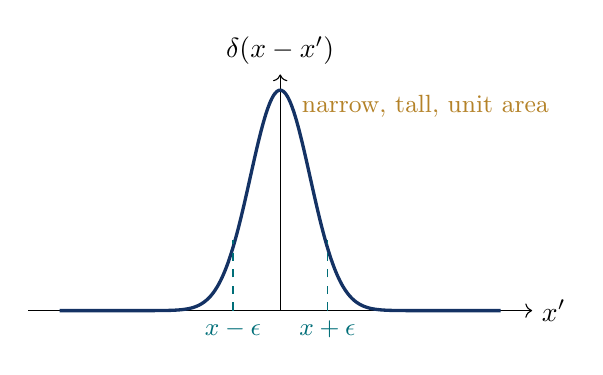
\begin{tikzpicture}[scale=1]
  \draw[->] (-3.2,0) -- (3.2,0) node[right] {$x'$};
  \draw[->] (0,0) -- (0,3.0) node[above] {$\delta(x-x')$};
  \draw[very thick,primary,domain=-2.8:2.8,samples=200,smooth] plot (\x,{2.8*exp(-(\x*\x)/(2*0.06*0.06*40))});
  \draw[dashed,secondary] (-0.6,0) -- (-0.6,0.9) (0.6,0) -- (0.6,0.9);
  \node[secondary,below] at (-0.6,0) {\small $x-\epsilon$};
  \node[secondary,below] at (0.6,0) {\small $x+\epsilon$};
  \node[exframe,right] at (0.15,2.6) {\small narrow, tall, unit area};
\end{tikzpicture}
\end{center}
\textbf{*** Study Note (the notebook's ``$=0$ for $x\neq x'$''):} The statement $\int dx'\,\delta(x-x')=0$ for $x\ne x'$ means the integration window does \emph{not} contain the singular point; with the window around $x'=x$ the integral is $1$. The delta function is not an ordinary function but a distribution: it acquires meaning only under an integral. A standard picture is a spike of width $\to0$ and height $\to\infty$ with area fixed at $1$, e.g.\ a Gaussian of vanishing width.

\textbf{*** Memory Rule:} ``Delta picks out the value.'' $\int dx'\,\delta(x-x')f(x')=f(x)$ replaces $x'$ by $x$ and removes the integral. The same rule gives $x'\delta(x-x')=x\,\delta(x-x')$.

\subsection{Derivative of the Delta Function}
Define $\delta'(x-x')=\dfrac d{dx}\delta(x-x')$. Acting on a function under the integral,
\begin{align*}
\int dx'\,\delta'(x-x')f(x')&=\int dx'\Big[\frac d{dx}\delta(x-x')\Big]f(x')
=\frac d{dx}\int dx'\,\delta(x-x')f(x')=\frac d{dx}f(x)=f'(x).
\end{align*}
\begin{thm}{Derivative of the Delta}
\begin{gather*}
\int dx'\,\delta'(x-x')f(x')=f'(x)=\int dx'\,\delta(x-x')f'(x'),\\
\text{i.e.}\quad \delta'(x-x')\ \equiv\ \delta(x-x')\frac d{dx'}\ \ (\text{under the integral}).
\end{gather*}
\end{thm}
\textbf{*** Verification:} Since $\delta(x-x')$ depends on $x-x'$, $\dfrac d{dx}\delta(x-x')=-\dfrac d{dx'}\delta(x-x')$. Integrating by parts (the boundary terms vanish because $\delta$ is zero away from $x'=x$), $\int dx'\big[-\partial_{x'}\delta(x-x')\big]f(x')=\int dx'\,\delta(x-x')f'(x')=f'(x)$, in agreement with the boxed identity.

\subsection{Eigenstates of Momentum}
The momentum matrix elements were postulated as $\langle x|\hat p|x'\rangle=-i\hbar\,\delta'(x-x')$. Write $\hat p=\hbar\hat k$ and denote the eigenfunction by $\langle x|k\rangle=\psi_k(x)$, so that $\langle x|\hat k|x'\rangle=-i\,\delta'(x-x')$ and $\hat k|k\rangle=k|k\rangle$. Then
\begin{align*}
\langle x|\hat k|k\rangle&=k\langle x|k\rangle\ \Rightarrow\ \int dx'\,\langle x|\hat k|x'\rangle\langle x'|k\rangle=k\,\langle x|k\rangle\\
&\Rightarrow\ \int dx'\,(-i)\,\delta'(x-x')\,\psi_k(x')=k\,\psi_k(x)\ \Rightarrow\ -i\int dx'\,\delta(x-x')\frac d{dx'}\psi_k(x')=k\,\psi_k(x),
\end{align*}
that is,
\[
-i\,\frac{d\psi_k(x)}{dx}=k\,\psi_k(x)\quad\Longrightarrow\quad\psi_k(x)=A\,e^{ikx}.
\]
To fix $A$, require $\langle k|k'\rangle=\delta(k-k')$ and insert $\int dx\,|x\rangle\langle x|=\mathbb 1$:
\[
\langle k|k'\rangle=\int dx\,\langle k|x\rangle\langle x|k'\rangle=|A|^2\int dx\,e^{-ikx}e^{ik'x}=|A|^2\int dx\,e^{-i(k-k')x}=|A|^2\,2\pi\,\delta(k-k').
\]
\begin{thm}{Momentum Eigenfunctions}
\[
\psi_k(x)=\langle x|k\rangle=\frac1{\sqrt{2\pi}}\,e^{ikx},\qquad \langle k|k'\rangle=\delta(k-k').
\]
\end{thm}
\textbf{*** Complete Solution (the delta function as a Fourier integral):} The identity used above, $\dfrac1{2\pi}\displaystyle\int_{-\infty}^\infty dx\,e^{-i(k-k')x}=\delta(k-k')$, is the statement that $\{e^{ikx}/\sqrt{2\pi}\}$ is a complete orthonormal set in the continuum sense. It is the same relation as $\delta(x-x')=\frac1{2\pi}\int dk\,e^{ik(x-x')}$. Choosing $A=1/\sqrt{2\pi}$ (a phase is arbitrary) gives the boxed normalization.

\subsection{Operators in the Position and Momentum Bases}
\textbf{Position basis.} Using $\int dx'\,|x'\rangle\langle x'|=\mathbb 1$ and the postulated matrix elements,
\begin{align*}
\langle x|\hat x|f\rangle&=\int dx'\,\langle x|\hat x|x'\rangle\langle x'|f\rangle=\int dx'\,x'\,\delta(x-x')f(x')=x\,f(x),\\
\langle x|\hat p|f\rangle&=\int dx'\,(-i\hbar)\,\delta'(x-x')f(x')=-i\hbar\,f'(x).
\end{align*}
Equivalently the matrix elements may be written
\begin{thm}{Position Basis}
\begin{gather*}
\langle x|\hat x|x'\rangle=x'\,\delta(x-x'),\qquad
\langle x|\hat p|x'\rangle=-i\hbar\,\delta(x-x')\frac d{dx'}\\
(\text{acting to the right on a function of }x'),
\end{gather*}
and in the $|x\rangle$ basis\quad $\hat x\equiv x,\quad \hat k\equiv-i\dfrac d{dx}\ (\hat p\equiv-i\hbar\dfrac d{dx})$.
\end{thm}

\textbf{Momentum basis.} Insert $\mathbb 1=\int dx\,|x\rangle\langle x|$ on both sides of $\hat x$:
\begin{align*}
\langle k|\hat x|k'\rangle&=\iint dx\,dx'\,\langle k|x\rangle\langle x|\hat x|x'\rangle\langle x'|k'\rangle
=\iint dx\,dx'\,\frac{e^{-ikx}}{\sqrt{2\pi}}\,x'\delta(x-x')\,\frac{e^{ik'x'}}{\sqrt{2\pi}}\\
&=\frac1{2\pi}\int dx\,e^{-ikx}\,x\,e^{ik'x}
=i\frac d{dk}\Big[\frac1{2\pi}\int dx\,e^{i(k'-k)x}\Big]=i\frac d{dk}\delta(k'-k)=i\,\delta'(k-k').
\end{align*}
\begin{thm}{Momentum Basis}
In the $|k\rangle$ basis\quad $\hat k\equiv k,\qquad \hat x\equiv i\dfrac d{dk}=i\hbar\dfrac d{dp}\quad(p=\hbar k)$.
\end{thm}
\textbf{*** Study Note (the $\hbar$ in the conversion):} Since $p=\hbar k$, $\dfrac d{dk}=\hbar\dfrac d{dp}$, so $i\dfrac d{dk}=i\hbar\dfrac d{dp}$. The position operator is a derivative in momentum space, just as the momentum operator is a derivative in position space. The notebook's conversion is written with an ambiguous $\hbar$; $i\hbar\,d/dp$ is the dimensionally correct form (position has the dimension of $\hbar/p$).

\subsection{The Canonical Commutator}
In the position representation, $\hat x|f\rangle\equiv x f(x)$ and $\hat p|f\rangle\equiv-i\hbar\dfrac{df}{dx}$. Then
\[
\hat x\hat p|f\rangle=-i\hbar\,x\frac{df}{dx},\qquad
\hat p\hat x|f\rangle=-i\hbar\frac d{dx}\big(xf\big)=-i\hbar f-i\hbar\,x\frac{df}{dx},
\qquad
(\hat x\hat p-\hat p\hat x)|f\rangle=i\hbar\,f .
\]
\begin{thm}{Canonical Commutation Relation}
\[
[\hat x,\hat p]=i\hbar,\qquad\text{hence}\qquad\Delta x\,\Delta p\ \ge\ \frac\hbar2 .
\]
\end{thm}
\textbf{*** Verification (momentum representation):} With $\hat k\equiv k$ and $\hat x\equiv i\,d/dk$, $[\hat x,\hat k]f=i\dfrac d{dk}(kf)-k\,i\dfrac{df}{dk}=i f$, so $[\hat x,\hat p]=\hbar\,[\hat x,\hat k]=i\hbar$ in either basis, as it must be since a commutator is basis independent.

\textbf{*** Exam Tip:} For any problem with a free particle, plane waves $e^{ikx}/\sqrt{2\pi}$ with $\hat p=\hbar\hat k$ are the basis, with $\langle k|k'\rangle=\delta(k-k')$. To change a wavefunction from position to momentum space, use $\phi(k)=\langle k|\psi\rangle=\int dx\,\langle k|x\rangle\psi(x)=\frac1{\sqrt{2\pi}}\int dx\,e^{-ikx}\psi(x)$.
%==============================================================================
\section{Time Evolution: Stationary States and the Schr\"odinger and Heisenberg Pictures}
\label{fd:sec:time}
%==============================================================================

\subsection{Postulate 4 and the Time-Evolution Operator}
\begin{thm}{Postulate 4: the Schr\"odinger Equation}
\[
i\hbar\,\frac d{dt}|\psi(t)\rangle=\hat H|\psi(t)\rangle,\qquad\text{equivalently}\qquad |\dot\psi(t)\rangle=-\frac i\hbar\hat H|\psi(t)\rangle .
\]
\end{thm}
Solving it involves three steps: (i) set up the equation, (ii) choose a general approach to its solution, (iii) choose a basis in which to solve it. The solution is written with the \emph{time-evolution operator} $\hat U(t)$:
\[
|\psi(t)\rangle=\hat U(t)|\psi(0)\rangle,\qquad |\dot\psi(0)\rangle=-\frac i\hbar\hat H|\psi(0)\rangle .
\]
\textbf{*** Study Note (notation):} The notebook writes the second relation as $|\psi(0)\rangle=-\frac i\hbar\hat H|\psi(0)\rangle$, which is not an identity; the dot (time derivative) on the left ket is the part that was lost. The correct statement is that the \emph{rate of change} of the state at $t=0$ is $-\frac i\hbar\hat H$ acting on the state.

\subsection{Time-Independent Hamiltonian: Solution in the Energy Basis}
Suppose $\dfrac{\partial\hat H}{\partial t}=0$, i.e.\ $\hat H$ does not depend explicitly on time, and let $\hat H|E\rangle=E|E\rangle$. Expand the state in this basis:
\[
|\psi(t)\rangle=\sum_E|E\rangle\langle E|\psi(t)\rangle=\sum_Ea_E(t)\,|E\rangle .
\]
Insert this in $\big(i\hbar\,\partial_t-\hat H\big)|\psi(t)\rangle=0$:
\[
\sum_E\big(i\hbar\,\dot a_E(t)-E\,a_E(t)\big)|E\rangle=0\ \Longrightarrow\ i\hbar\,\dot a_E(t)=E\,a_E(t),
\]
since the $|E\rangle$ are linearly independent. The solution is $a_E(t)=a_E(0)\,e^{-iEt/\hbar}$.

\begin{thm}{Solution for a Time-Independent Hamiltonian}
\begin{align*}
\langle E|\psi(t)\rangle&=\langle E|\psi(0)\rangle\,e^{-iEt/\hbar},\qquad
|\psi(t)\rangle=\Big[\sum_Ee^{-iEt/\hbar}|E\rangle\langle E|\Big]|\psi(0)\rangle\\
\hat U(t)&=\sum_Ee^{-iEt/\hbar}|E\rangle\langle E|\quad(\text{non-degenerate}),\\
\hat U(t)&=\sum_{E,\alpha}e^{-iEt/\hbar}|E,\alpha\rangle\langle E,\alpha|\quad(\text{degenerate}).
\end{align*}
\end{thm}
Since $\hat H|E\rangle=E|E\rangle$, we have $e^{-iEt/\hbar}|E\rangle=e^{-i\hat Ht/\hbar}|E\rangle$, and therefore
\[
\hat U(t)=\sum_Ee^{-i\hat Ht/\hbar}|E\rangle\langle E|=e^{-i\hat Ht/\hbar}\sum_E|E\rangle\langle E|=e^{-i\hat Ht/\hbar}.
\]
\begin{thm}{The Time-Evolution Operator}
\[
\hat U(t)=\exp\Big(-\frac{i\hat Ht}\hbar\Big),\qquad \hat U\hat U^\dagger=\hat U^\dagger\hat U=\mathbb 1\quad(\text{unitary}).
\]
\end{thm}
\textbf{*** Complete Solution (unitarity):} Using $\langle E|E'\rangle=\delta_{EE'}$,
\[
\hat U^\dagger\hat U=\sum_{E,E'}e^{iEt/\hbar}e^{-iE't/\hbar}|E\rangle\langle E|E'\rangle\langle E'|=\sum_E|E\rangle\langle E|=\mathbb 1 .
\]
Consequently
\[
\langle\psi(t)|\psi(t)\rangle=\langle\psi(0)|\hat U^\dagger\hat U|\psi(0)\rangle=\langle\psi(0)|\psi(0)\rangle,
\]
so the total probability does not change in time. Unitarity is the mathematical form of probability conservation.

\subsubsection*{Stationary states}
If the system starts in a single energy eigenstate (including the degenerate case), $|\psi(0)\rangle=|E\rangle$, then
\[
|\psi(t)\rangle=|\psi(0)\rangle\,e^{-iEt/\hbar},\qquad
|\langle E|\psi(t)\rangle|^2=\big|\langle E|\psi(0)\rangle\,e^{-iEt/\hbar}\big|^2=|\langle E|\psi(0)\rangle|^2 .
\]
The probabilities of all measurements are independent of time. These are the \emph{stationary states}. Only the phase $e^{-iEt/\hbar}$ changes, and a global phase has no physical consequence.

\textbf{*** Intuition:} A general state is a superposition of energy eigenstates, each rotating in the complex plane at its own angular frequency $E/\hbar$. Interference between components with different $E$ is what produces genuine time dependence; a single component alone gives a frozen probability distribution.

\textbf{*** Study Note (choice of basis):} For a Hamiltonian such as $\hat H=\dfrac{\hat p^2}{2m}+\dfrac1{\cosh^2x}$, the potential is a function of position, so solving in the $x$-basis (a differential equation) is easier than in any basis where $\hat x$ is not diagonal. Choose the basis in which the Hamiltonian is simplest.

\textbf{*** Exam Tip:} To find $|\psi(t)\rangle$: (1) find the eigenstates $|E\rangle$ of $\hat H$, (2) expand $|\psi(0)\rangle=\sum_Ec_E|E\rangle$ with $c_E=\langle E|\psi(0)\rangle$, (3) attach $e^{-iEt/\hbar}$ to each term. Probabilities of measuring energy $E$ never change; probabilities of measuring other observables generally do.

\subsection{The Schr\"odinger Picture}
In the Schr\"odinger picture the state vectors depend on time and the operators are time independent:
\[
i\hbar\frac d{dt}|\psi(t)\rangle=\hat H|\psi(t)\rangle,\qquad |\psi(t)\rangle=\hat U(t)|\psi(0)\rangle=\hat U(t,t_0)|\psi(t_0)\rangle,\qquad \hat U(t)=e^{-i\hat Ht/\hbar},\ \ \hat U^\dagger\hat U=\mathbb 1 .
\]

\subsection{The Heisenberg Picture}
Invert the evolution: $|\psi(0)\rangle=\hat U^\dagger(t)|\psi(t)\rangle$. Define the Heisenberg state
\[
|\psi\rangle_H\equiv|\psi(0)\rangle=e^{i\hat Ht/\hbar}|\psi(t)\rangle ,
\]
which is \emph{frozen in time}. The expectation value of an operator $\hat A$ (which is time independent in the Schr\"odinger picture) is
\[
\langle\psi(t)|\hat A|\psi(t)\rangle=\langle\psi(0)|\,e^{i\hat Ht/\hbar}\hat A\,e^{-i\hat Ht/\hbar}\,|\psi(0)\rangle=\langle\psi(0)|\hat A_H|\psi(0)\rangle=\ _H\langle\psi|\hat A_H|\psi\rangle_H ,
\]
which defines the time-dependent Heisenberg operator.
\begin{thm}{Heisenberg Operator}
\[
\hat A_H(t)=\hat U^\dagger\hat A\,\hat U=e^{i\hat Ht/\hbar}\,\hat A\,e^{-i\hat Ht/\hbar}\qquad\Big(\text{with }\frac{\partial\hat A}{\partial t}=0\Big).
\]
\end{thm}
To find its equation of motion, note $\hat U^\dagger=e^{i\hat Ht/\hbar}$ and $\hat U=e^{-i\hat Ht/\hbar}$ give
\[
\frac{\partial\hat U^\dagger}{\partial t}=\hat U^\dagger\,\frac i\hbar\hat H,\qquad
\frac{\partial\hat U}{\partial t}=-\hat U\,\frac i\hbar\hat H .
\]
Then
\begin{align*}
\frac{d\hat A_H}{dt}&=\frac{\partial\hat U^\dagger}{\partial t}\hat A\hat U+\hat U^\dagger\hat A\frac{\partial\hat U}{\partial t}
=\frac i\hbar\,\hat U^\dagger\hat H\hat A\hat U-\frac i\hbar\,\hat U^\dagger\hat A\hat U\hat H\\
&=\frac i\hbar\Big[\hat U^\dagger\hat H\hat U\ \hat U^\dagger\hat A\hat U-\hat U^\dagger\hat A\hat U\ \hat U^\dagger\hat H\hat U\Big]
=\frac i\hbar\big[\hat H,\hat A_H\big]=\frac1{i\hbar}\big[\hat A_H,\hat H\big],
\end{align*}
where we inserted $\hat U\hat U^\dagger=\mathbb 1$ and used $\hat U^\dagger\hat H\hat U=\hat H$.
\begin{thm}{Heisenberg Equation of Motion}
\[
\frac{d\hat A_H}{dt}=\frac1{i\hbar}\big[\hat A_H,\hat H\big]\qquad\text{and}\qquad\frac d{dt}\langle\hat A\rangle=\frac1{i\hbar}\big\langle[\hat A,\hat H]\big\rangle .
\]
\end{thm}
\textbf{Note:} A unitary transformation by $\hat U=e^{-i\hat Ht/\hbar}$ does not change the Hamiltonian, since $\hat U^\dagger\hat H\hat U=\hat U^\dagger\hat U\hat H=\hat H$ (it commutes with its own exponential).

\textbf{*** Intuition:} In the Schr\"odinger picture the state moves and the measuring apparatus is fixed; in the Heisenberg picture the state is fixed and the operators rotate. Both give identical expectation values and probabilities. The Heisenberg form is the quantum counterpart of the classical equation $\dot A=\{A,H\}$ with the Poisson bracket replaced by $\frac1{i\hbar}[\ ,\ ]$.

\textbf{*** Complete Solution (conservation laws):} If $[\hat A,\hat H]=0$ then $d\langle\hat A\rangle/dt=0$ and $\hat A$ is conserved. For $\hat A=\hat H$ itself, $[\hat H,\hat H]=0$, so $\langle\hat H\rangle$ (the energy) is conserved when $\hat H$ has no explicit time dependence.

\begin{prob}{Worked Example: Free Particle in the Heisenberg Picture}
Find $\hat x_H(t)$ and $\hat p_H(t)$ for $\hat H=\hat p^2/2m$.
\end{prob}
\textbf{*** Complete Solution:} Since $[\hat p,\hat H]=0$, $\dfrac{d\hat p_H}{dt}=0$, so $\hat p_H(t)=\hat p$. For the position, $[\hat x,\hat p^2]=\hat p[\hat x,\hat p]+[\hat x,\hat p]\hat p=2i\hbar\hat p$, hence
\[
\frac{d\hat x_H}{dt}=\frac1{i\hbar}\frac{[\hat x,\hat p^2]}{2m}=\frac{\hat p}m\quad\Longrightarrow\quad \hat x_H(t)=\hat x+\frac{\hat p}m\,t .
\]
\textbf{*** Verification:} This is the classical straight-line motion $x=x_0+(p/m)t$, and $[\hat x_H(t),\hat p_H(t)]=[\hat x,\hat p]=i\hbar$ is preserved at all times, as it must be for a unitary transformation.

\begin{center}
\renewcommand{\arraystretch}{1.2}
\begin{tabular}{@{}lll@{}}
\toprule
 & \textbf{Schr\"odinger picture} & \textbf{Heisenberg picture}\\
\midrule
State & $|\psi(t)\rangle=\hat U(t)|\psi(0)\rangle$ & $|\psi\rangle_H=|\psi(0)\rangle$ (frozen)\\
Operator & $\hat A$ (fixed) & $\hat A_H(t)=\hat U^\dagger\hat A\hat U$\\
Equation & $i\hbar\,\partial_t|\psi\rangle=\hat H|\psi\rangle$ & $\dot{\hat A}_H=\frac1{i\hbar}[\hat A_H,\hat H]$\\
Expectation value & $\langle\psi(t)|\hat A|\psi(t)\rangle$ & $\ _H\langle\psi|\hat A_H(t)|\psi\rangle_H$ (the same number)\\
\bottomrule
\end{tabular}
\end{center}
%==============================================================================
\section{The One-Dimensional Time-Independent Schr\"odinger Equation}
\label{fd:sec:onedim}
%==============================================================================

\subsection{The Equation and the Classification of Spectra}
For a time-independent one-dimensional potential $V(x)$ and total energy $E$,
\begin{gather*}
-\frac{\hbar^2}{2m}\frac{d^2\psi(x)}{dx^2}+V(x)\,\psi(x)=E\,\psi(x),\\
\psi(x,t)=\psi(x,0)\,e^{-iEt/\hbar},\qquad |\psi(x,t)|^2=|\psi(x,0)|^2\ \ (\text{stationary state}).
\end{gather*}
Consider a potential with different asymptotic values, $V(-\infty)=V_1$ and $V(+\infty)=V_2$ with $V_1<V_2$, and a minimum $V_{\min}$.

\begin{center}
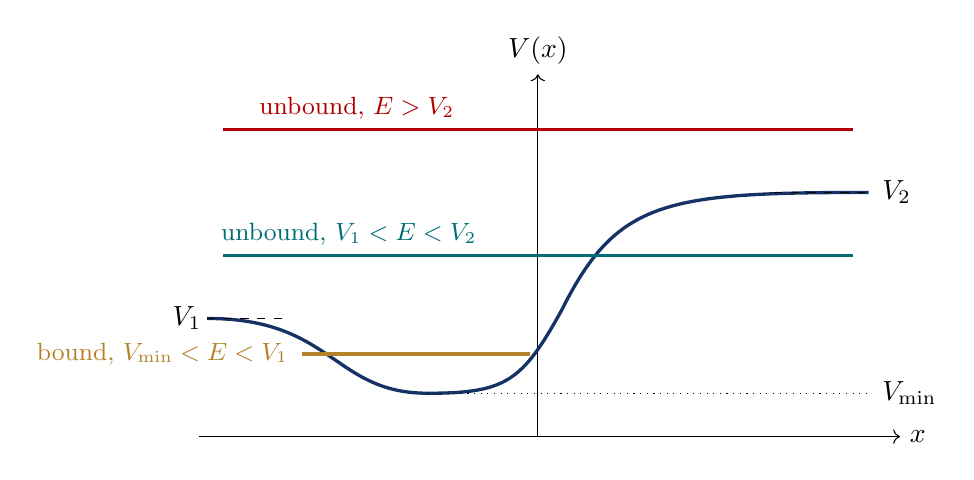
\begin{tikzpicture}[scale=1]
  \draw[->] (-4.3,0) -- (4.6,0) node[right] {$x$};
  \draw[->] (0,0) -- (0,4.6) node[above] {$V(x)$};
  \draw[very thick,primary] (-4.2,1.5) .. controls (-2.6,1.5) and (-2.6,0.55) .. (-1.4,0.55) .. controls (-0.4,0.55) and (-0.2,0.7) .. (0.3,1.6) .. controls (1.0,3.0) and (1.6,3.1) .. (4.2,3.1);
  \draw[dashed] (-4.2,1.5) -- (-3.2,1.5); \node[left] at (-4.15,1.5) {$V_1$};
  \draw[dashed] (3.0,3.1) -- (4.2,3.1);   \node[right] at (4.25,3.1) {$V_2$};
  \draw[dotted] (-1.4,0.55) -- (4.2,0.55); \node[right] at (4.25,0.55) {$V_{\min}$};
  \draw[exframe,very thick] (-3.0,1.05) -- (-0.1,1.05); \node[exframe,left] at (-3.05,1.05) {\small bound, $V_{\min}<E<V_1$};
  \draw[secondary,very thick] (-4.0,2.3) -- (4.0,2.3); \node[secondary,above] at (-2.4,2.3) {\small unbound, $V_1<E<V_2$};
  \draw[red!70!black,very thick] (-4.0,3.9) -- (4.0,3.9); \node[red!70!black,above] at (-2.3,3.9) {\small unbound, $E>V_2$};
\end{tikzpicture}
\end{center}

\subsection{(A) Discrete Spectrum: Bound States}
Bound states occur whenever the particle cannot move to infinity: it is confined, at that energy, to a finite region of space bounded by the classical turning points. This requires
\[
V_{\min}<E<V_1,\qquad \psi(x)\to0\ \text{ at }x=\pm\infty,
\]
i.e.\ the energy is below the asymptotic value of the potential on both sides. For bound states to exist, $V(x)$ must have at least one minimum lower than $V_1$. The energy spectrum is then discrete.

\begin{thm}{Theorem 1 (bound states)}
In a one-dimensional problem the energy levels of bound states are discrete and non-degenerate.
\end{thm}
\begin{thm}{Theorem 2 (nodes)}
The wavefunction $\psi_n(x)$ of a one-dimensional bound-state system has $n$ nodes if $n=0$ labels the ground state, and $(n-1)$ nodes if $n=1$ labels the ground state.
\end{thm}
\textbf{*** Complete Solution (non-degeneracy, Theorem 1):} Let $\psi_1,\psi_2$ be two bound-state solutions with the same $E$. From $\psi''=\frac{2m}{\hbar^2}(V-E)\psi$,
\[
\psi_1''\psi_2-\psi_2''\psi_1=0\ \Longrightarrow\ \frac d{dx}\big(\psi_1'\psi_2-\psi_2'\psi_1\big)=0 ,
\]
so the Wronskian $W=\psi_1'\psi_2-\psi_2'\psi_1$ is constant. Both functions vanish at $x\to\infty$, so $W=0$ everywhere. Then $\psi_1'/\psi_1=\psi_2'/\psi_2$, hence $\psi_2=c\,\psi_1$: the two solutions are the same state. Discreteness has a physical origin: a solution that decays at $+\infty$ and one that decays at $-\infty$ can be joined smoothly only for special energies, so the allowed $E$ form a discrete set.

\textbf{*** Verification (nodes):} For the infinite square well of width $L$, $\psi_n=\sqrt{2/L}\sin(n\pi x/L)$ with $n=1,2,\dots$ (ground state $n=1$) has $n-1$ interior nodes. For the harmonic oscillator (Section~\ref{fd:sec:sho}) with ground state $n=0$, $\psi_n$ has $n$ nodes. Both agree with Theorem 2, the first with the ``$n=1$ is the ground state'' labelling and the second with ``$n=0$''.

\textbf{*** Intuition:} Higher energy means shorter local wavelength, so the wavefunction oscillates more and picks up more zeros. The ground state is always nodeless and every state above it gains one node.

\subsection{(B) Continuous Spectrum: Unbound States}
\begin{itemize}[itemsep=2pt]
\item[(i)] $V_1<E<V_2$: the particle can escape only to $x\to-\infty$ (on the right it is in a classically forbidden region). The energy spectrum is continuous and non-degenerate.
\item[(ii)] $E>V_2$: the particle can escape in both directions. The energy spectrum is continuous and doubly degenerate.
\end{itemize}
\textbf{*** Complete Solution (why the degeneracies differ):} For $E>V_2$ both asymptotic regions are classically allowed, so at each end the wavefunction is oscillatory and may be a combination of left- and right-moving waves, giving two independent solutions (e.g.\ a wave incident from the left and a wave incident from the right) at the same energy: doubly degenerate. For $V_1<E<V_2$ the solution must decay on the right, which removes one of the two independent solutions and leaves a single one at each $E$: non-degenerate.

\textbf{*** Exam Tip:} Quick classification: compare $E$ with $V(\pm\infty)$. Below both: discrete and non-degenerate (bound). Between the two limits: continuous and non-degenerate. Above both: continuous and doubly degenerate.
%==============================================================================
\section{The Linear Harmonic Oscillator: Ladder-Operator Method}
\label{fd:sec:sho}
%==============================================================================

\subsection{Hamiltonian and the Operators \texorpdfstring{$\hat a,\hat a^\dagger$}{a and a-dagger}}
\[
\hat H=\frac{\hat p^2}{2m}+\frac12m\omega^2\hat x^2,\qquad \hat H|\psi\rangle=E|\psi\rangle .
\]
Define the \emph{annihilation} and \emph{creation} operators
\[
\hat a=\frac1{\sqrt{2m\hbar\omega}}\big(m\omega\hat x+i\hat p\big),\qquad
\hat a^\dagger=\frac1{\sqrt{2m\hbar\omega}}\big(m\omega\hat x-i\hat p\big),
\]
which invert to
\[
\hat x=\sqrt{\frac\hbar{2m\omega}}\,\big(\hat a+\hat a^\dagger\big),\qquad
\hat p=i\sqrt{\frac{m\hbar\omega}2}\,\big(\hat a^\dagger-\hat a\big).
\]
\textbf{Commutator.} Starting from $[\hat x,\hat p]=i\hbar$,
\begin{align*}
[\hat x,\hat p]&=\Big[\sqrt{\tfrac\hbar{2m\omega}}(\hat a^\dagger+\hat a),\ i\sqrt{\tfrac{m\hbar\omega}2}(\hat a^\dagger-\hat a)\Big]
=\frac{i\hbar}2\big[(\hat a^\dagger+\hat a),(\hat a^\dagger-\hat a)\big]\\
&=\frac{i\hbar}2\Big\{[\hat a,\hat a^\dagger]-[\hat a,\hat a]+[\hat a^\dagger,\hat a^\dagger]-[\hat a^\dagger,\hat a]\Big\}
=\frac{i\hbar}2\cdot2[\hat a,\hat a^\dagger]=i\hbar\,[\hat a,\hat a^\dagger].
\end{align*}
\begin{thm}{Ladder-Operator Algebra}
\[
[\hat a,\hat a^\dagger]=1,\qquad [\hat a,\hat a]=[\hat a^\dagger,\hat a^\dagger]=0 .
\]
\end{thm}
\textbf{*** Study Note:} Here $[\hat a^\dagger,\hat a]=-[\hat a,\hat a^\dagger]=-1$ was used in the line above to combine the first and last terms. The whole algebra of the oscillator follows from this single commutator.

\subsection{The Hamiltonian in Terms of \texorpdfstring{$\hat a^\dagger\hat a$}{a-dagger a}}
\begin{align*}
\hat a^\dagger\hat a&=\frac1{2m\hbar\omega}\big(m\omega\hat x-i\hat p\big)\big(m\omega\hat x+i\hat p\big)
=\frac{m\omega\hat x^2}{2\hbar}+\frac{\hat p^2}{2m\hbar\omega}+\frac i{2\hbar}[\hat x,\hat p]
=\frac{\hat H}{\hbar\omega}-\frac12\mathbb 1 .
\end{align*}
\begin{thm}{Oscillator Hamiltonian}
\[
\hat H=\Big(\hat a^\dagger\hat a+\frac12\Big)\hbar\omega,\qquad\text{or in units of }\hbar\omega:\quad
\hat{\mathcal H}\equiv\frac{\hat H}{\hbar\omega}=\hat a^\dagger\hat a+\frac12,\quad \hat{\mathcal H}|\epsilon\rangle=\epsilon|\epsilon\rangle .
\]
\end{thm}
\textbf{*** Study Note:} The cross terms $\hat x\hat p$ and $\hat p\hat x$ combine into $\frac i{2\hbar}[\hat x,\hat p]=\frac i{2\hbar}(i\hbar)=-\frac12$, which is the origin of the $\frac12$. The ``zero-point'' term $\frac12\hbar\omega$ is a purely quantum effect coming from $[\hat x,\hat p]\neq0$.

\subsection{Raising and Lowering the Energy}
Compute the commutators with $\hat{\mathcal H}=\hat a^\dagger\hat a+\frac12$:
\[
[\hat a,\hat{\mathcal H}]=[\hat a,\hat a^\dagger\hat a]=[\hat a,\hat a^\dagger]\hat a+\hat a^\dagger[\hat a,\hat a]=\hat a,\qquad
[\hat a^\dagger,\hat{\mathcal H}]=[\hat a^\dagger,\hat a^\dagger\hat a]=\hat a^\dagger[\hat a^\dagger,\hat a]=-\hat a^\dagger .
\]
Hence, using $\hat{\mathcal H}\hat a=\hat a\hat{\mathcal H}-[\hat a,\hat{\mathcal H}]$,
\[
\hat{\mathcal H}\,\hat a|\epsilon\rangle=\big(\hat a\hat{\mathcal H}-\hat a\big)|\epsilon\rangle=(\epsilon-1)\,\hat a|\epsilon\rangle,
\qquad\text{and similarly}\qquad
\hat{\mathcal H}\,\hat a^\dagger|\epsilon\rangle=(\epsilon+1)\,\hat a^\dagger|\epsilon\rangle .
\]
\begin{thm}{Ladder Property}
\[
\hat a|\epsilon\rangle=c_\epsilon|\epsilon-1\rangle\ \ (\text{lowering operator}),\qquad
\hat a^\dagger|\epsilon\rangle=c'_\epsilon|\epsilon+1\rangle\ \ (\text{raising operator}).
\]
\end{thm}
\textbf{*** Intuition:} $\hat a$ takes an energy eigenstate to another eigenstate one quantum $\hbar\omega$ lower; $\hat a^\dagger$ takes it one quantum higher. Like climbing a ladder with equal rungs, one only needs the bottom rung and the rule for stepping up.

\subsection{The Ground State and the Spectrum}
Let $|\epsilon_0\rangle$ be the lowest state, so that lowering cannot go further: $\hat a|\epsilon_0\rangle=0$. Then $\hat a^\dagger\hat a|\epsilon_0\rangle=0$, i.e.\ $\big(\hat{\mathcal H}-\frac12\big)|\epsilon_0\rangle=0$, so
\[
\hat{\mathcal H}|\epsilon_0\rangle=\tfrac12|\epsilon_0\rangle\ \Longrightarrow\ \epsilon_0=\tfrac12,\qquad E_0=\tfrac12\hbar\omega .
\]
Applying the raising operator repeatedly gives $\epsilon_1=\big(1+\frac12\big)\hbar\omega=\frac32\hbar\omega$, and so on.

\textbf{*** Complete Solution (why a lowest state must exist):} For any eigenstate, $\langle\epsilon|\hat a^\dagger\hat a|\epsilon\rangle=\|\hat a|\epsilon\rangle\|^2\ge0$, i.e.\ $\epsilon-\frac12\ge0$, so $\epsilon\ge\frac12$. If repeated lowering never terminated, $\epsilon-1,\epsilon-2,\dots$ would eventually fall below $\frac12$, a contradiction. So lowering must stop at a state with $\hat a|\epsilon_0\rangle=0$, which fixes $\epsilon_0=\frac12$; the allowed values are then $\epsilon_0+n$ with $n=0,1,2,\dots$ (no values in between, since one cannot stop lowering at any other $\epsilon$).

\begin{thm}{Energy Spectrum}
\[
E_n=\Big(n+\frac12\Big)\hbar\omega,\qquad n=0,1,2,\dots,\qquad
\hat H|n\rangle=\Big(n+\frac12\Big)\hbar\omega|n\rangle .
\]
\end{thm}
\begin{center}
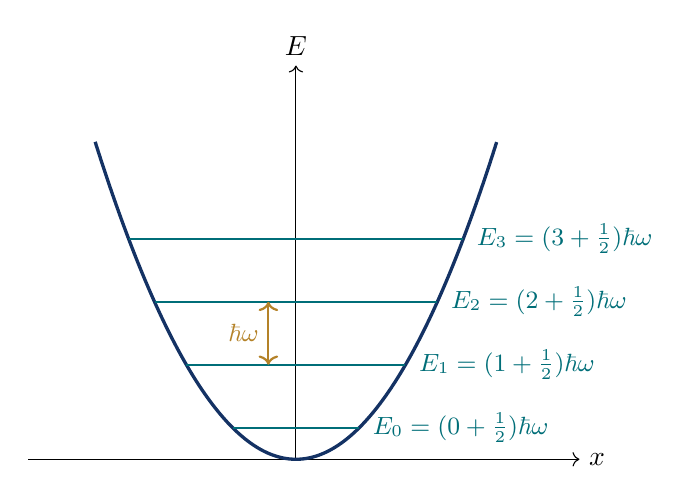
\begin{tikzpicture}[scale=1]
  \draw[->] (-3.4,0) -- (3.6,0) node[right] {$x$};
  \draw[->] (0,0) -- (0,5.0) node[above] {$E$};
  \draw[very thick,primary,domain=-2.55:2.55,samples=80,smooth] plot (\x,{0.62*\x*\x});
  \foreach \n in {0,1,2,3} {
    \pgfmathsetmacro{\e}{0.8*(\n+0.5)+0.0}
    \draw[secondary,thick] ({-sqrt(\e/0.62)},\e) -- ({sqrt(\e/0.62)},\e);
    \node[right,secondary] at ({sqrt(\e/0.62)+0.05},\e) {\small $E_\n=(\n+\tfrac12)\hbar\omega$};
  }
  \draw[<->,exframe,thick] (-0.35,1.2) -- (-0.35,2.0); \node[exframe,left] at (-0.35,1.6) {\small $\hbar\omega$};
\end{tikzpicture}
\end{center}
\textbf{*** Study Note (figure):} The levels are equally spaced by $\hbar\omega$, with the lowest at $\frac12\hbar\omega$, not $0$. Each level $E_n$ is non-degenerate, as Theorem 1 of Section~\ref{fd:sec:onedim} requires for a bound state in one dimension.

\subsection{Normalization of the Ladder Action}
Write $\hat a|n\rangle=c_n|n-1\rangle$ (so $\hat a^\dagger$ has the adjoint action $\langle n|\hat a^\dagger=c_n^*\langle n-1|$). Then
\[
\langle n|\hat a^\dagger\hat a|n\rangle=|c_n|^2\ \Rightarrow\ \langle n|\big(\hat{\mathcal H}-\tfrac12\big)|n\rangle=|c_n|^2\ \Rightarrow\ n\langle n|n\rangle=|c_n|^2\ \Rightarrow\ c_n=\sqrt n
\]
(taking the phase of $|n-1\rangle$ so that $c_n$ is real and positive).
\begin{thm}{Action of $\hat a,\hat a^\dagger$ and the Number Operator}
\[
\hat a|n\rangle=\sqrt n\,|n-1\rangle,\qquad \hat a^\dagger|n\rangle=\sqrt{n+1}\,|n+1\rangle,\qquad
\hat a^\dagger\hat a|n\rangle=n|n\rangle .
\]
$\hat N\equiv\hat a^\dagger\hat a$ is the \emph{number operator}, $\hat H=\hbar\omega\big(\hat N+\frac12\big)$ and $[\hat H,\hat N]=0$.
\end{thm}
\textbf{*** Verification (the raising coefficient):} $\langle n+1|\hat a^\dagger|n\rangle=\langle n|\hat a|n+1\rangle^*=\sqrt{n+1}$, so $\hat a^\dagger|n\rangle=\sqrt{n+1}|n+1\rangle$. Combining, $\hat a^\dagger\hat a|n\rangle=\sqrt n\sqrt n|n\rangle=n|n\rangle$ \checkmark.

\subsubsection*{Matrix representation}
\[
\langle n'|\hat a|n\rangle=\sqrt n\,\delta_{n',n-1},\qquad \langle n'|\hat a^\dagger|n\rangle=\sqrt{n+1}\,\delta_{n',n+1}.
\]
\textbf{*** Complete Solution (the matrix the notebook starts):} In the basis $|0\rangle,|1\rangle,|2\rangle,|3\rangle,\dots$ (rows $n'$, columns $n$),
\[
\hat a^\dagger=\begin{pmatrix}0&0&0&0&\cdots\\ 1&0&0&0&\cdots\\ 0&\sqrt2&0&0&\cdots\\ 0&0&\sqrt3&0&\cdots\\ \vdots&\vdots&\vdots&\vdots&\ddots\end{pmatrix},\qquad
\hat a=(\hat a^\dagger)^T=\begin{pmatrix}0&1&0&0&\cdots\\ 0&0&\sqrt2&0&\cdots\\ 0&0&0&\sqrt3&\cdots\\ 0&0&0&0&\cdots\\ \vdots&\vdots&\vdots&\vdots&\ddots\end{pmatrix}.
\]
In the notebook's table the first listed column is $|1\rangle$ (the state $|0\rangle$ is not shown), which is why the first row is $0$ and the next entry is $\sqrt2$: the table starts one step up the ladder. With $|0\rangle$ included the first sub-diagonal entry is $\langle1|\hat a^\dagger|0\rangle=1$.

\subsection{Constructing All States from the Ground State}
From $\hat a^\dagger|0\rangle=|1\rangle$, $\hat a^\dagger|1\rangle=\sqrt2\,|2\rangle$:
\[
|2\rangle=\frac1{\sqrt2}\hat a^\dagger|1\rangle=\frac1{\sqrt{2\cdot1}}(\hat a^\dagger)^2|0\rangle=\frac1{\sqrt{2!}}(\hat a^\dagger)^2|0\rangle .
\]
\begin{thm}{Number States from the Vacuum}
\[
|n\rangle=\frac1{\sqrt{n!}}\big(\hat a^\dagger\big)^n|0\rangle=\frac1{\sqrt{n!}}\Big[\frac1{\sqrt{2m\hbar\omega}}\big(m\omega\hat x-i\hat p\big)\Big]^n|0\rangle .
\]
\end{thm}

\subsection{Wavefunctions in the Position Basis}
\textbf{Ground state.} Use $\hat a|0\rangle=0$ and project onto $\langle x|$, with $\hat p\to-i\hbar\,d/dx$:
\begin{align*}
\langle x|\big(m\omega\hat x+i\hat p\big)|0\rangle&=\int dx'\,\langle x|m\omega\hat x|x'\rangle\langle x'|0\rangle+i\!\int dx'\,\langle x|\hat p|x'\rangle\langle x'|0\rangle\\
&=\Big[m\omega x+i\Big(-i\hbar\frac d{dx}\Big)\Big]\langle x|0\rangle=0
\ \Longrightarrow\ \Big(m\omega x+\hbar\frac d{dx}\Big)\psi_0(x)=0 .
\end{align*}
Separating variables, $\dfrac{d\psi_0}{\psi_0}=-\dfrac{m\omega}\hbar x\,dx$, so
\[
\psi_0(x)=N\exp\Big(-\frac{m\omega}{2\hbar}x^2\Big),\qquad N=\Big(\frac{m\omega}{\pi\hbar}\Big)^{1/4},
\]
where $N$ follows from $\int|\psi_0|^2dx=N^2\sqrt{\pi\hbar/m\omega}=1$.

\textbf{Excited states.} Substituting $\hat p\to-i\hbar\,d/dx$ in $|n\rangle=\frac1{\sqrt{n!}}(\hat a^\dagger)^n|0\rangle$:
\begin{thm}{Oscillator Eigenfunctions}
\[
\langle x|n\rangle=\psi_n(x)=\frac1{(2m\hbar\omega)^{n/2}}\Big(m\omega x-\hbar\frac d{dx}\Big)^n\frac{\psi_0(x)}{\sqrt{n!}}
\]
These are the Hermite functions: $\psi_n$ is a polynomial of degree $n$ (a Hermite polynomial) times the Gaussian $e^{-m\omega x^2/2\hbar}$.
\end{thm}
\textbf{*** Complete Solution (first excited state):} Since $\hbar\psi_0'=-m\omega x\,\psi_0$, we get $\big(m\omega x-\hbar\frac d{dx}\big)\psi_0=2m\omega x\,\psi_0$, hence
\[
\psi_1(x)=\frac{2m\omega\,x}{\sqrt{2m\hbar\omega}}\psi_0(x)=\sqrt{\frac{2m\omega}\hbar}\;x\,\psi_0(x)=\sqrt{\frac{2m\omega}\hbar}\Big(\frac{m\omega}{\pi\hbar}\Big)^{1/4}x\,e^{-m\omega x^2/2\hbar},
\]
which is odd, has one node at $x=0$ (consistent with Theorem 2 of Section~\ref{fd:sec:onedim}), and is normalized: $\int|\psi_1|^2dx=\frac{2m\omega}\hbar N^2\int x^2e^{-m\omega x^2/\hbar}dx=\frac{2m\omega}\hbar N^2\cdot\frac{\hbar}{2m\omega}\sqrt{\frac{\pi\hbar}{m\omega}}=1$ \checkmark.

\subsection{Moments and the Uncertainty Product}
In the state $|n\rangle$, $\langle\hat x\rangle=\sqrt{\frac\hbar{2m\omega}}\langle n|\hat a+\hat a^\dagger|n\rangle=0$ since $\hat a,\hat a^\dagger$ change $n$, and likewise $\langle\hat p\rangle=0$. Hence $(\Delta p)^2=\langle\hat p^2\rangle$ and $(\Delta x)^2=\langle\hat x^2\rangle$. Squaring the definitions,
\begin{align*}
\langle\hat p^2\rangle&=-\frac{m\hbar\omega}2\big\langle n\big|\hat a^\dagger\hat a^\dagger-\hat a^\dagger\hat a-\hat a\hat a^\dagger+\hat a\hat a\big|n\big\rangle
=\frac{m\hbar\omega}2\big\langle n\big|\hat a^\dagger\hat a+\hat a\hat a^\dagger\big|n\big\rangle\\
&=\frac{m\hbar\omega}2\big\langle n\big|2\hat a^\dagger\hat a+1\big|n\big\rangle=\frac{m\hbar\omega}2(2n+1)=m\hbar\omega\Big(n+\frac12\Big),
\end{align*}
because $\hat a^\dagger\hat a^\dagger$ and $\hat a\hat a$ change $n$ by $\pm2$ and have zero diagonal elements, and $\hat a\hat a^\dagger=\hat a^\dagger\hat a+1$. In the same way
\[
\langle\hat x^2\rangle=\frac\hbar{2m\omega}\langle n|\hat a^\dagger\hat a+\hat a\hat a^\dagger|n\rangle=\frac\hbar{m\omega}\Big(n+\frac12\Big).
\]
\begin{thm}{Uncertainty in the Oscillator States}
\[
\Delta x\,\Delta p=\Big(n+\frac12\Big)\hbar,\qquad\text{ground state }(n=0):\ \ \Delta x\,\Delta p=\frac\hbar2\ \ (\text{minimum uncertainty}).
\]
\end{thm}
\textbf{*** Verification (virial theorem):} $\langle T\rangle=\dfrac{\langle\hat p^2\rangle}{2m}=\dfrac12\hbar\omega\big(n+\frac12\big)$ and $\langle V\rangle=\dfrac12m\omega^2\langle\hat x^2\rangle=\dfrac12\hbar\omega\big(n+\frac12\big)$, so $\langle T\rangle=\langle V\rangle=\frac12E_n$ and their sum is $E_n$ \checkmark.

\textbf{*** Memory Rule:} Ladder rules: $\hat a|n\rangle=\sqrt n|n-1\rangle$ (the factor is $\sqrt{\text{the larger index}}$ in both $\hat a$ and $\hat a^\dagger$ matrix elements), $\hat a^\dagger|n\rangle=\sqrt{n+1}|n+1\rangle$, $\hat N=\hat a^\dagger\hat a$, and $[\hat a,\hat a^\dagger]=1$.

\textbf{*** Exam Tip:} For any matrix element of $\hat x^k\hat p^l$ between number states, replace $\hat x,\hat p$ by $\hat a,\hat a^\dagger$, expand, and keep only terms with equal numbers of $\hat a$ and $\hat a^\dagger$ (diagonal elements) or the right net difference (off-diagonal). Reorder with $\hat a\hat a^\dagger=\hat a^\dagger\hat a+1$.
%==============================================================================
\section{Classical Limit of the Oscillator: Coherent States}
\label{fd:sec:coh}
%==============================================================================

\subsection{Construction and Eigenvalue Property}
The number states $|n\rangle$ have $\langle x\rangle=0$ at all times and no classical motion, so they do not resemble a classical oscillator. A state that does is built as a superposition of all number states with Poisson-like weights.

\begin{thm}{Coherent State}
\[
|\alpha\rangle=\exp\Big(-\frac12|\alpha|^2\Big)\sum_{n=0}^\infty\frac{\alpha^n}{\sqrt{n!}}\,|n\rangle,\qquad\alpha\in\mathbb C .
\]
$|\alpha\rangle$ is an eigenstate of the annihilation operator: $\ \hat a|\alpha\rangle=\alpha|\alpha\rangle$.
\end{thm}
\textbf{Proof.} Using $\hat a|n\rangle=\sqrt n|n-1\rangle$ (the $n=0$ term is killed by $\hat a$),
\begin{align*}
\hat a|\alpha\rangle&=e^{-|\alpha|^2/2}\sum_{n=0}^\infty\frac{\alpha^n}{\sqrt{n!}}\hat a|n\rangle
=e^{-|\alpha|^2/2}\sum_{n=1}^\infty\frac{\alpha^n}{\sqrt{n!}}\sqrt n\,|n-1\rangle\\
&=\alpha\,e^{-|\alpha|^2/2}\sum_{n=1}^\infty\frac{\alpha^{n-1}}{\sqrt{(n-1)!}}|n-1\rangle=\alpha|\alpha\rangle .\ \blacksquare
\end{align*}
\textbf{Normalization.} Using $\langle m|n\rangle=\delta_{mn}$,
\[
\langle\alpha|\alpha\rangle=e^{-|\alpha|^2}\sum_{m,n}\frac{(\alpha^*)^m\alpha^n}{\sqrt{m!\,n!}}\langle m|n\rangle=e^{-|\alpha|^2}\sum_{n=0}^\infty\frac{|\alpha|^{2n}}{n!}=e^{-|\alpha|^2}e^{|\alpha|^2}=1 .
\]
\textbf{*** Intuition:} $\hat a$ is not Hermitian, so its eigenvalue $\alpha$ is a complex number, with no restriction. The real and imaginary parts of $\alpha$ will turn out to encode the mean position and mean momentum, so $\alpha$ is a point in classical phase space.

\textbf{*** Complete Solution (photon-number statistics):} The probability of finding $n$ quanta is $P(n)=|\langle n|\alpha\rangle|^2=e^{-|\alpha|^2}\dfrac{|\alpha|^{2n}}{n!}$, a Poisson distribution with mean $\bar n=\langle\alpha|\hat a^\dagger\hat a|\alpha\rangle=|\alpha|^2$ and width $\Delta n=|\alpha|$. The energy is $\langle\hat H\rangle=\hbar\omega(|\alpha|^2+\frac12)$. For large $|\alpha|$ the relative spread $\Delta n/\bar n=1/|\alpha|\to0$, which is the classical limit of a well-defined energy.

\subsection{Position, Momentum and Uncertainty}
Since $\hat a|\alpha\rangle=\alpha|\alpha\rangle$, taking the adjoint gives $\langle\alpha|\hat a^\dagger=\langle\alpha|\alpha^*$. With $\hat x=\sqrt{\frac\hbar{2m\omega}}(\hat a^\dagger+\hat a)$ and $\hat p=i\sqrt{\frac{m\hbar\omega}2}(\hat a^\dagger-\hat a)$:
\begin{align*}
\langle\hat x\rangle&=\langle\alpha|\hat x|\alpha\rangle=\sqrt{\frac\hbar{2m\omega}}\,\langle\alpha|\hat a^\dagger+\hat a|\alpha\rangle=\sqrt{\frac\hbar{2m\omega}}\,(\alpha+\alpha^*),\\
\langle\hat x^2\rangle&=\frac\hbar{2m\omega}\langle\alpha|\hat a^{\dagger2}+\hat a^2+\hat a\hat a^\dagger+\hat a^\dagger\hat a|\alpha\rangle\\
&=\frac\hbar{2m\omega}\langle\alpha|\hat a^{\dagger2}+\hat a^2+2\hat a^\dagger\hat a+1|\alpha\rangle
=\frac\hbar{2m\omega}\big(\alpha^{*2}+\alpha^2+2\alpha^*\alpha+1\big).
\end{align*}
Therefore $(\Delta x)^2=\langle\hat x^2\rangle-\langle\hat x\rangle^2=\dfrac\hbar{2m\omega}$, since $\langle\hat x\rangle^2=\frac\hbar{2m\omega}(\alpha^2+\alpha^{*2}+2\alpha^*\alpha)$.

\textbf{*** Complete Solution (momentum, left out in the notebook):}
\begin{align*}
\langle\hat p\rangle&=i\sqrt{\tfrac{m\hbar\omega}2}\,(\alpha^*-\alpha)=\sqrt{2m\hbar\omega}\,\mathrm{Im}\,\alpha,\\
\langle\hat p^2\rangle&=-\frac{m\hbar\omega}2\big(\alpha^{*2}+\alpha^2-2|\alpha|^2-1\big),\qquad
\langle\hat p\rangle^2=-\frac{m\hbar\omega}2\big(\alpha^{*2}+\alpha^2-2|\alpha|^2\big),
\end{align*}
so $(\Delta p)^2=\dfrac{m\hbar\omega}2$. The same $\Delta x$ and $\Delta p$ hold for every $\alpha$ and equal the ground-state values.

\begin{thm}{Coherent States are Minimum-Uncertainty States}
\[
(\Delta x)^2=\frac\hbar{2m\omega},\qquad(\Delta p)^2=\frac{m\hbar\omega}2,\qquad(\Delta x)^2(\Delta p)^2=\frac{\hbar^2}4,\qquad
\boxed{\Delta x\,\Delta p=\frac\hbar2}\ \text{ for coherent states.}
\]
\end{thm}
Coherent states saturate the uncertainty bound, so they are as close to a classical point in phase space as quantum mechanics permits.

\textbf{*** Study Note:} The ground state is the special case $\alpha=0$, i.e.\ $|\alpha=0\rangle=|0\rangle$. A general coherent state is the ground-state Gaussian displaced in phase space: it has the same width but its centre sits at $\langle x\rangle,\langle p\rangle$ set by $\alpha$.

\textbf{*** Complete Solution (the wavefunction):} In the position basis $\hat a|\alpha\rangle=\alpha|\alpha\rangle$ becomes $\big(m\omega x+\hbar\frac d{dx}\big)\psi_\alpha=\sqrt{2m\hbar\omega}\,\alpha\,\psi_\alpha$, whose solution is
\[
\psi_\alpha(x)\propto\exp\Big[-\frac{m\omega}{2\hbar}(x-x_0)^2+\frac i\hbar p_0x\Big],\qquad
x_0=\sqrt{\frac{2\hbar}{m\omega}}\,\mathrm{Re}\,\alpha,\quad p_0=\sqrt{2m\hbar\omega}\,\mathrm{Im}\,\alpha ,
\]
which is the ground-state Gaussian centred at $x_0$ with mean momentum $p_0$, in agreement with $\langle\hat x\rangle=x_0$ and $\langle\hat p\rangle=p_0$ above.

\textbf{*** Study Note (overlaps):} Coherent states are not orthogonal. From the definition, $\langle\beta|\alpha\rangle=\exp\big(-\tfrac12|\alpha|^2-\tfrac12|\beta|^2+\beta^*\alpha\big)$ and $|\langle\beta|\alpha\rangle|^2=e^{-|\alpha-\beta|^2}$, which is small only when $|\alpha-\beta|$ is large. They form an overcomplete set. The notebook marks further work on coherent states as an exercise from Sakurai; the overlap and the photon-number distribution above are the standard first parts of it.

\subsection{Time Evolution of a Coherent State}
Apply the time-evolution operator $\hat U(t)=e^{-i\hat Ht/\hbar}$, which acts on $|n\rangle$ as $e^{-i(n+\frac12)\omega t}$:
\[
|\alpha(t)\rangle=\hat U(t)|\alpha\rangle=e^{-|\alpha|^2/2}\sum_{n=0}^\infty\frac{\alpha^n}{\sqrt{n!}}\,e^{-i(n+\frac12)\omega t}|n\rangle
=e^{-i\omega t/2}\,\big|\alpha e^{-i\omega t}\big\rangle .
\]
\begin{thm}{A Coherent State Stays Coherent}
\[
|\alpha(t)\rangle=e^{-i\omega t/2}\,|\alpha e^{-i\omega t}\rangle .
\]
\end{thm}
Up to a global phase, the label $\alpha$ simply rotates clockwise in the complex plane with angular frequency $\omega$.
\textbf{*** Verification:} In the last step, $e^{-|\alpha|^2/2}\sum\frac{\alpha^n}{\sqrt{n!}}e^{-in\omega t}|n\rangle=e^{-|\alpha e^{-i\omega t}|^2/2}\sum\frac{(\alpha e^{-i\omega t})^n}{\sqrt{n!}}|n\rangle$ because $|\alpha e^{-i\omega t}|=|\alpha|$.

\textbf{Expectation value of $\hat x$.} The direct double sum gives (using $\langle m|\hat a^\dagger|n\rangle=\sqrt{n+1}\,\delta_{m,n+1}$ and $\langle m|\hat a|n\rangle=\sqrt n\,\delta_{m,n-1}$)
\begin{align*}
\langle x(t)\rangle&=\langle\alpha(t)|\hat x|\alpha(t)\rangle
=\sqrt{\frac\hbar{2m\omega}}\,e^{-|\alpha|^2}\sum_{m,n}\frac{\alpha^{*m}\alpha^n}{\sqrt{m!\,n!}}\langle m|\hat a^\dagger+\hat a|n\rangle\,e^{-i\omega t(n-m)}\\
&=\sqrt{\frac\hbar{2m\omega}}\,e^{-|\alpha|^2}\Big[\sum_n\frac{\alpha^{*(n-1)}\alpha^n}{(n-1)!}e^{-i\omega t}+\sum_n\frac{\alpha^{*(n+1)}\alpha^n}{n!}e^{i\omega t}\Big]\\
&=\sqrt{\frac\hbar{2m\omega}}\,e^{-|\alpha|^2}\Big[\alpha\,e^{|\alpha|^2}e^{-i\omega t}+\alpha^*\,e^{|\alpha|^2}e^{i\omega t}\Big].
\end{align*}
Write $\alpha=|\alpha|e^{i\delta}$. Then $\alpha e^{-i\omega t}=|\alpha|e^{-i(\omega t-\delta)}$ and
\begin{thm}{Classical Motion of the Mean Position}
\[
\langle x(t)\rangle=\sqrt{\frac\hbar{2m\omega}}\,|\alpha|\Big[e^{-i(\omega t-\delta)}+e^{i(\omega t-\delta)}\Big]=2\sqrt{\frac\hbar{2m\omega}}\,|\alpha|\cos(\omega t-\delta)=A\cos(\omega t-\delta),
\]
\[
\frac{d^2}{dt^2}\langle x(t)\rangle=-\omega^2\langle x(t)\rangle .
\]
\end{thm}
Here $A=2\sqrt{\hbar/2m\omega}\,|\alpha|$ is the classical amplitude and $\delta$ a phase constant: the mean position obeys the equation of the classical harmonic oscillator.

\begin{center}
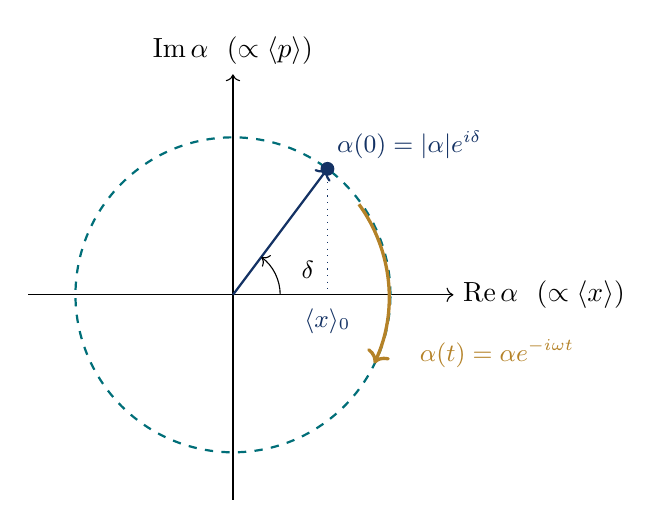
\begin{tikzpicture}[scale=1]
  \draw[->] (-2.6,0) -- (2.8,0) node[right] {$\mathrm{Re}\,\alpha\ \ (\propto\langle x\rangle)$};
  \draw[->] (0,-2.6) -- (0,2.8) node[above] {$\mathrm{Im}\,\alpha\ \ (\propto\langle p\rangle)$};
  \draw[secondary,thick,dashed] (0,0) circle (2);
  \fill[primary] (1.2,1.6) circle (2.5pt) node[above right] {\small $\alpha(0)=|\alpha|e^{i\delta}$};
  \draw[->,primary,thick] (0,0) -- (1.2,1.6);
  \draw[->,exframe,very thick] (1.6,1.15) arc (36:-25:2.0);
  \node[exframe,right] at (2.25,-0.75) {\small $\alpha(t)=\alpha e^{-i\omega t}$};
  \draw[dotted,primary] (1.2,1.6) -- (1.2,0); \node[below,primary] at (1.2,-0.05) {\small $\langle x\rangle_0$};
  \draw[->] (0.6,0) arc (0:53:0.6);
  \node at (0.95,0.32) {\small $\delta$};
\end{tikzpicture}
\end{center}
\textbf{*** Study Note (figure):} The point $\alpha(t)$ circles the origin clockwise with angular frequency $\omega$; its projections on the two axes are (up to constants) $\langle x(t)\rangle$ and $\langle p(t)\rangle$, which is the classical phase-space ellipse of the oscillator. The width of the packet does not change, so the quantum state follows the classical trajectory without spreading, which is the sense in which coherent states are the closest quantum analogue of a classical oscillator.

\textbf{*** Verification (Ehrenfest):} From Section~\ref{fd:sec:time}, $\frac d{dt}\langle\hat x\rangle=\frac1{i\hbar}\langle[\hat x,\hat H]\rangle=\langle\hat p\rangle/m$ and $\frac d{dt}\langle\hat p\rangle=-m\omega^2\langle\hat x\rangle$, so $\frac{d^2}{dt^2}\langle\hat x\rangle=-\omega^2\langle\hat x\rangle$ for \emph{every} state. The new content for a coherent state is that the packet stays a minimum-uncertainty Gaussian while this happens.

\textbf{*** Exam Tip:} Three quick facts to quote: (i) $\hat a|\alpha\rangle=\alpha|\alpha\rangle$ with $\alpha$ complex; (ii) $\Delta x\,\Delta p=\hbar/2$ for all $\alpha$; (iii) $|\alpha(t)\rangle=e^{-i\omega t/2}|\alpha e^{-i\omega t}\rangle$, so $\langle x(t)\rangle=A\cos(\omega t-\delta)$. For the time-evolution calculation, it is faster to use $\langle x\rangle=\sqrt{\hbar/2m\omega}\,(\alpha(t)+\alpha^*(t))$ than the double sum.


%%% PART 2
\partheading{Symmetry, Angular Momentum and Clebsch-Gordan Coefficients}{This part covers symmetry and conservation laws in quantum mechanics: translation and time translation (momentum and energy conservation, the time-evolution operator), rotations and the angular momentum algebra, spin-$\tfrac12$ and the Pauli matrices, the $j=1$ representation, rotation matrices, orbital angular momentum and spherical harmonics, addition of angular momenta with Clebsch-Gordan coefficients, spin-orbit coupling (the sodium doublet, the Zeeman and Paschen-Back limits) and central potentials.}




%==============================================================================
\section{Translation Symmetry and Conservation of Momentum}
\label{sy:sec:trans}
%==============================================================================

\subsection{How States Transform Under a Translation}
Let $\vec r$ be a dynamical variable. A translation by $\vec a$ moves a point according to
\[
\vec r'=\hat T(\vec a)\vec r=\vec r+\vec a,\qquad \vec r=\hat T(\vec a)^{-1}\vec r'=\vec r'-\vec a .
\]
The state vector transforms as $|\psi'\rangle=\hat U_T(\vec a)|\psi\rangle$. Because space is homogeneous, the value of the wavefunction is carried along with the point, so
\[
\psi'(\vec r')=\psi(\vec r)\quad\Longrightarrow\quad \hat U_T(\vec a)\psi(\vec r')=\psi\big(\hat T(\vec a)^{-1}\vec r'\big)=\psi(\vec r'-\vec a).
\]
Renaming the dummy variable gives the defining action
\[
\hat U_T(\vec a)\,\psi(\vec r)=\psi(\vec r-\vec a).
\]

\subsection{The Generator of Translations}
Take an infinitesimal translation $\delta\vec a$ and Taylor expand:
\begin{align*}
\hat U_T(\delta\vec a)\psi(\vec r)&=\psi(\vec r-\delta\vec a)=\psi(\vec r)-\delta\vec a\cdot\vec\nabla\psi(\vec r)\\
&=\psi(\vec r)-\frac{i}{\hbar}\,\delta\vec a\cdot\hat{\vec p}\,\psi(\vec r)=\Big[\mathbb 1-\frac i\hbar\,\delta\vec a\cdot\hat{\vec p}\Big]\psi(\vec r),
\end{align*}
using $\hat{\vec p}=-i\hbar\vec\nabla$.

\begin{thm}{Momentum Generates Translations}
\[
\hat U_T(\delta\vec a)=\mathbb 1-\frac i\hbar\,\delta\vec a\cdot\hat{\vec p}.
\]
\end{thm}

Build a finite translation from $n$ small ones, $\delta\vec a=\vec a/n$:
\[
\hat U_T(\vec a)=\lim_{n\to\infty}\Big[\mathbb 1-\frac i\hbar\,\frac{\vec a}{n}\cdot\hat{\vec p}\Big]^n.
\]

\begin{thm}{Finite Translation Operator}
\[
\hat U_T(\vec a)=\exp\!\Big(-\frac i\hbar\,\vec a\cdot\hat{\vec p}\Big).
\]
\end{thm}

If $|\psi\rangle$ is an eigenstate of momentum, $\hat{\vec p}|\psi\rangle=\vec p\,|\psi\rangle$, then
\[
|\psi'\rangle=\hat U_T(\vec a)|\psi\rangle=\exp\!\Big(-\frac i\hbar\,\vec a\cdot\vec p\Big)|\psi\rangle .
\]
The state acquires only a phase. Two consequences follow: a momentum eigenstate is unchanged (up to a phase) by a translation, and conversely a state that does not change under translation must be an eigenstate of the momentum operator.

\textbf{*** Intuition:} A plane wave $e^{i\vec p\cdot\vec r/\hbar}$ looks the same everywhere, so sliding it sideways changes nothing physical. That is exactly why it can be an eigenstate of the translation generator.

\subsection{Invariance of the Hamiltonian}
Operators transform as $\hat H'=\hat U_T\hat H\hat U_T^\dagger$. For an infinitesimal translation,
\begin{align*}
\hat H'&=\Big[\mathbb 1-\frac i\hbar\,\delta\vec a\cdot\hat{\vec p}\Big]\hat H\Big[\mathbb 1+\frac i\hbar\,\delta\vec a\cdot\hat{\vec p}\Big]\\
&=\hat H-\frac i\hbar\,\delta\vec a\cdot\hat{\vec p}\,\hat H+\frac i\hbar\,\hat H\,\delta\vec a\cdot\hat{\vec p}
=\hat H+\frac i\hbar\,\delta\vec a\cdot[\hat H,\hat{\vec p}\,].
\end{align*}
If the Hamiltonian is invariant under translation, $\hat H'=\hat H$, then $[\hat H,\hat{\vec p}\,]=0$.

For any observable $\hat A$ without explicit time dependence,
\[
\frac{d}{dt}\langle\hat A\rangle=\frac1{i\hbar}\langle[\hat A,\hat H]\rangle ,
\]
so $[\hat A,\hat H]=0$ implies that $\langle\hat A\rangle$ is conserved.

\begin{thm}{Homogeneity of Space $\Rightarrow$ Momentum Conservation}
\[
[\hat H,\hat{\vec p}\,]=0\quad\Longrightarrow\quad \frac{d}{dt}\langle\hat{\vec p}\,\rangle=0 .
\]
\end{thm}

\textbf{*** Study Note:} The recipe used throughout this chapter is the same each time. (i) Find the unitary operator for the symmetry, $\hat U=\exp(-\tfrac i\hbar\,\text{parameter}\times\text{generator})$. (ii) Require $\hat U\hat H\hat U^\dagger=\hat H$, which is equivalent to $[\hat H,\text{generator}]=0$. (iii) Conclude that the expectation value of the generator is conserved. Translation gives $\hat{\vec p}$, time translation will give $\hat H$ and rotation will give $\hat{\vec L}$.

\textbf{*** Exam Tip:} The sign in $\hat U_T(\vec a)\psi(\vec r)=\psi(\vec r-\vec a)$ is a frequent source of errors. The state is moved by $+\vec a$, so the new wavefunction at $\vec r$ takes the old value from $\vec r-\vec a$.

%==============================================================================
\section{Time Translation and the Time-Evolution Operator}
\label{sy:sec:time}
%==============================================================================

\subsection{Definition of \texorpdfstring{$\hat U(t,t_0)$}{U(t,t0)}}
The Schr\"odinger equation is
\[
i\hbar\frac{\partial}{\partial t}|\psi(t)\rangle=\hat H|\psi(t)\rangle .
\]
The state at a later time $t>t_0$ is related to the initial state by a linear operator,
\[
|\psi(t)\rangle=\hat U(t,t_0)|\psi(t_0)\rangle,\qquad \hat U(t_0,t_0)=\mathbb 1 .
\]
Substituting into the Schr\"odinger equation, and noting that $|\psi(t_0)\rangle$ is arbitrary,
\[
i\hbar\frac{\partial}{\partial t}\hat U(t,t_0)=\hat H\,\hat U(t,t_0)
\quad\Longleftrightarrow\quad
\frac{\partial}{\partial t}\hat U(t,t_0)=-\frac i\hbar\hat H\,\hat U(t,t_0).
\]
Integrating from $t_0$ to $t$ and using $\hat U(t_0,t_0)=\mathbb 1$ gives the integral equation
\[
\hat U(t,t_0)=\mathbb 1-\frac i\hbar\int_{t_0}^{t}\hat H\,\hat U(t',t_0)\,dt' .
\]

\begin{thm}{Unitarity of $\hat U$}
\[
\langle\psi(t)|\psi(t)\rangle=\langle\psi(t_0)|\psi(t_0)\rangle\quad\Longrightarrow\quad \hat U^\dagger\hat U=\mathbb 1 .
\]
\end{thm}

\textbf{*** Study Note:} The norm is conserved because $\hat H$ is Hermitian, since $\frac{d}{dt}\langle\psi|\psi\rangle=\frac{i}{\hbar}\langle\psi|(\hat H^\dagger-\hat H)|\psi\rangle=0$. A time-dependent Hermitian $\hat H$ also gives a unitary $\hat U$; only the closed form below needs $\hat H$ independent of time.

\subsection{The Generator of Time Translation}
Look at a short step $\delta t$ after $t_0$. From the differential equation,
\[
i\hbar\big[\hat U(t_0+\delta t,t_0)-\hat U(t_0,t_0)\big]=\hat H\,\hat U(t_0+\delta t,t_0)\,\delta t ,
\]
so, with $\hat U(t_0,t_0)=\mathbb 1$,
\[
\hat U(t_0+\delta t,t_0)=\mathbb 1-\frac i\hbar\hat H\Big[\hat U(t_0,t_0)+\frac{\partial\hat U}{\partial t}\Big|_{t=t_0}\delta t+\cdots\Big]\delta t=\mathbb 1-\frac i\hbar\hat H\,\delta t+O(\delta t^2).
\]
Dropping the $O(\delta t^2)$ term defines the infinitesimal time translation.

\begin{thm}{Hamiltonian Generates Time Translations}
\[
\hat U_T(\delta t)=\mathbb 1-\frac i\hbar\,\hat H\,\delta t .
\]
\end{thm}

Compare with $\hat U_T(\delta\vec a)=\mathbb 1-\tfrac i\hbar\,\delta\vec a\cdot\hat{\vec p}$: the Hamiltonian plays for time the role that momentum plays for space.

\subsection{The Finite Time-Evolution Operator}
Take $\hat H$ independent of time and split $t-t_0$ into $n$ steps of size $\delta t=(t-t_0)/n$:
\[
\hat U(t,t_0)=\lim_{n\to\infty}\Big[\mathbb 1-\frac i\hbar\,\frac{t-t_0}{n}\,\hat H\Big]^n .
\]

\begin{thm}{Time-Evolution Operator for a Time-Independent $\hat H$}
\[
\hat U(t,t_0)=\exp\!\Big[-\frac i\hbar\,\hat H\,(t-t_0)\Big].
\]
\end{thm}

\subsection{Energy Conservation}
Under a time translation the Hamiltonian transforms as
\[
\hat H'=\Big(\mathbb 1-\frac i\hbar\hat H\,\delta t\Big)\hat H\Big(\mathbb 1+\frac i\hbar\hat H\,\delta t\Big)=\hat H ,
\]
because $\hat H$ commutes with itself. Using the general rule $\frac{d}{dt}\langle\hat A\rangle=\frac1{i\hbar}\langle[\hat A,\hat H]\rangle$ with $\hat A=\hat H$,

\begin{thm}{Time Translation Invariance $\Rightarrow$ Energy Conservation}
\[
\frac{d}{dt}\langle\hat H\rangle=\frac1{i\hbar}\langle[\hat H,\hat H]\rangle=0 .
\]
\end{thm}

\textbf{*** Intuition:} If the laws of physics do not change with the clock, the energy is conserved. This is the third member of the family: homogeneity of space gives momentum, isotropy gives angular momentum and homogeneity of time gives energy.

\textbf{*** Memory Rule:} The generator multiplies the parameter, always with $-\tfrac i\hbar$: $\ \hat U=\exp\!\big(-\tfrac i\hbar\ \mathrm{parameter}\times\mathrm{generator}\big)$. Space shift $\to\vec a\cdot\hat{\vec p}$, time shift $\to t\,\hat H$, rotation $\to\phi\,\hat n\cdot\hat{\vec L}$.

\begin{prob}{Stationary-State Evolution}
\textbf{*** Complete Solution:} Let $\hat H|E_n\rangle=E_n|E_n\rangle$ and $|\psi(t_0)\rangle=\sum_nc_n|E_n\rangle$. Then
\[
|\psi(t)\rangle=e^{-i\hat H(t-t_0)/\hbar}\sum_nc_n|E_n\rangle=\sum_nc_n\,e^{-iE_n(t-t_0)/\hbar}|E_n\rangle .
\]
The probabilities $|c_n|^2$ do not depend on time, which is the statement that the energy distribution is conserved. A single eigenstate only picks up a phase, so every expectation value in a stationary state is constant.
\end{prob}

%==============================================================================
\section{Rotations, Isotropy of Space and Angular Momentum Conservation}
\label{sy:sec:rot}
%==============================================================================

\subsection{Rotation of a State}
The state vector is $|\psi\rangle$ and its position-space representation is $\langle\vec r|\psi\rangle=\psi(\vec r)$. A rotation takes a point to $\vec r'=\hat R(\phi)\vec r$, and the state to $\psi'(\vec r)=\hat U_R(\phi)\psi(\vec r)$ (the notes use $U_R(\phi)\equiv D_R(\phi)$ for the same operator). Isotropy of space means the wavefunction value travels with the point:
\[
\psi'(\vec r')=\psi(\vec r)\quad\Longrightarrow\quad \hat U_R(\phi)\psi(\vec r)=\psi\big(\hat R^{-1}(\phi)\vec r\big).
\]
For a rotation about the $z$-axis by the angle $\phi$,
\[
\begin{pmatrix}x'\\y'\\z'\end{pmatrix}=\underbrace{\begin{pmatrix}\cos\phi&-\sin\phi&0\\ \sin\phi&\cos\phi&0\\0&0&1\end{pmatrix}}_{\hat R_z(\phi)}\begin{pmatrix}x\\y\\z\end{pmatrix}.
\]

\subsection{Rotation About the \texorpdfstring{$z$}{z}-Axis}
For an infinitesimal angle $\delta\phi$ the matrix and its inverse are
\[
\hat R_z(\delta\phi)=\begin{pmatrix}1&-\delta\phi&0\\ \delta\phi&1&0\\0&0&1\end{pmatrix},\qquad
\hat R_z^{-1}(\delta\phi)=\begin{pmatrix}1&\delta\phi&0\\-\delta\phi&1&0\\0&0&1\end{pmatrix}.
\]
Therefore
\begin{align*}
\hat U_{R_z}(\delta\phi)\psi(\vec r)&=\psi\big(\hat R_z^{-1}(\delta\phi)\vec r\big)=\psi(x+\delta\phi\,y,\,-\delta\phi\,x+y,\,z)\\
&=\psi(x,y,z)+\delta\phi\Big(y\frac{\partial}{\partial x}-x\frac{\partial}{\partial y}\Big)\psi(x,y,z)\\
&=\Big[\mathbb 1-\frac i\hbar\,\delta\phi\,(x\hat p_y-y\hat p_x)\Big]\psi(x,y,z).
\end{align*}
The combination $x\hat p_y-y\hat p_x$ is $\hat L_z$, which therefore generates rotations about $z$.

\begin{thm}{Infinitesimal Rotation About $z$}
\[
\hat U_{R_z}(\delta\phi)=\mathbb 1-\frac i\hbar\,\delta\phi\,\hat L_z .
\]
\end{thm}

With $\delta\phi=\phi/N$,
\[
\hat U_{R_z}(\phi)=\lim_{N\to\infty}\Big(\mathbb 1-\frac i\hbar\frac\phi N\hat L_z\Big)^N=\exp\!\Big(-\frac i\hbar\,\hat L_z\phi\Big).
\]

\subsection{Rotation About a General Axis}
For a rotation about the unit vector $\hat n$ through a small angle,
\[
\vec r'=\hat R_{\hat n}(\delta\phi)\vec r=\vec r+\delta\phi\,(\hat n\times\vec r),
\]
so
\begin{align*}
\hat U_{R_{\hat n}}(\delta\phi)\psi(\vec r)&=\psi\big(\hat R_{\hat n}^{-1}\vec r\big)=\psi\big(\vec r-\delta\phi\,(\hat n\times\vec r)\big)\\
&=\Big[\mathbb 1-\delta\phi\ \hat n\cdot(\vec r\times\vec\nabla)\Big]\psi(\vec r)=\Big[\mathbb 1-\frac i\hbar\,\delta\phi\ \hat n\cdot\hat{\vec L}\Big]\psi(\vec r),
\end{align*}
using $\hat n\cdot(\vec r\times\vec\nabla)=\tfrac i\hbar\,\hat n\cdot\hat{\vec L}$ with $\hat{\vec L}=\vec r\times\hat{\vec p}$.

\begin{center}
\begin{tikzpicture}[scale=1.0,>=Stealth]
\draw[->] (0,0)--(0,3) node[above]{$z$};
\draw[->] (0,0)--(3.2,0) node[right]{$y$};
\draw[->] (0,0)--(-1.6,-1.4) node[below left]{$x$};
\draw[->,very thick,primary] (0,0)--(1.9,1.9) node[above right]{$\hat n$};
\draw[->,secondary,thick] (1.2,1.55) arc[start angle=140,end angle=-100,x radius=0.35,y radius=0.28];
\node[secondary,right] at (1.7,1.1) {rotation by $\phi$};
\end{tikzpicture}
\end{center}

\begin{thm}{Rotation Operators}
\[
\hat U_{R_{\hat n}}(\delta\phi)=\mathbb 1-\frac i\hbar\,\delta\phi\ \hat n\cdot\hat{\vec L},\qquad
\hat U_{R_{\hat n}}(\phi)=\exp\!\Big(-\frac i\hbar\,\phi\ \hat n\cdot\hat{\vec L}\Big).
\]
Angular momentum is the generator of rotations.
\end{thm}

\subsection{Isotropy and Conservation of Angular Momentum}
Under a rotation $\hat H'=\hat U_{R_{\hat n}}\hat H\hat U_{R_{\hat n}}^\dagger$. For an infinitesimal rotation,
\[
\hat H'=\Big[\mathbb 1-\frac i\hbar\,\delta\phi\,\hat n\cdot\hat{\vec L}\Big]\hat H\Big[\mathbb 1+\frac i\hbar\,\delta\phi\,\hat n\cdot\hat{\vec L}\Big]=\hat H+\frac i\hbar\,\delta\phi\ \hat n\cdot[\hat H,\hat{\vec L}\,]+O(\delta\phi^2).
\]
If $\hat H$ is invariant, $\hat H'=\hat H$ for every $\hat n$, so
\begin{thm}{Isotropy of Space $\Rightarrow$ Angular Momentum Conservation}
\[
[\hat H,\hat{\vec L}\,]=0\quad\Longrightarrow\quad \langle\hat{\vec L}\,\rangle\ \text{is conserved.}
\]
\end{thm}

\subsection{Non-Commutation of Rotations: the Angular Momentum Algebra}
Rotations about different axes do not commute, and this fixes the commutators of the generators. Take two infinitesimal rotations of equal angle $\delta\phi$, about $x$ and about $y$, with unit vectors $\hat e_1$ and $\hat e_2$. First,
\begin{align*}
\hat U_y(\delta\phi)\hat U_x(\delta\phi)\psi(\vec r)&=\psi\big((\hat R_y\hat R_x)^{-1}\vec r\big)=\psi\big(\hat R_x^{-1}\hat R_y^{-1}\vec r\big)\\
&=\psi\big(\hat R_x^{-1}[\vec r-\delta\phi(\hat e_2\times\vec r)]\big)\\
&=\psi\Big[\vec r-\delta\phi(\hat e_2\times\vec r)-\delta\phi\,\hat e_1\times\{\vec r-\delta\phi(\hat e_2\times\vec r)\}\Big]\\
&=\psi\Big[\vec r-\delta\phi(\hat e_1+\hat e_2)\times\vec r+\delta\phi^2\,\hat e_1\times(\hat e_2\times\vec r)\Big].
\end{align*}
Similarly, with the order reversed,
\[
\hat U_x(\delta\phi)\hat U_y(\delta\phi)\psi(\vec r)=\psi\Big[\vec r-\delta\phi(\hat e_1+\hat e_2)\times\vec r+\delta\phi^2\,\hat e_2\times(\hat e_1\times\vec r)\Big].
\]
Subtract the two and keep terms to order $\delta\phi^2$:
\begin{align*}
\big[\hat U_x(\delta\phi),\hat U_y(\delta\phi)\big]\psi(\vec r)&=\delta\phi^2\big[\hat e_2\times(\hat e_1\times\vec r)-\hat e_1\times(\hat e_2\times\vec r)\big]\cdot\vec\nabla\psi\\
&=\delta\phi^2\,[\,y\,\hat e_1-x\,\hat e_2\,]\cdot\vec\nabla\psi=-\delta\phi^2\,\frac i\hbar\,\hat L_z\,\psi(\vec r).\tag{I}
\end{align*}
On the other hand, expanding the operators directly,
\begin{align*}
\big[\hat U_x,\hat U_y\big]\psi&=\Big[\Big(\mathbb 1-\tfrac i\hbar\delta\phi\hat L_x\Big)\Big(\mathbb 1-\tfrac i\hbar\delta\phi\hat L_y\Big)-\Big(\mathbb 1-\tfrac i\hbar\delta\phi\hat L_y\Big)\Big(\mathbb 1-\tfrac i\hbar\delta\phi\hat L_x\Big)\Big]\psi\\
&=-\frac{\delta\phi^2}{\hbar^2}[\hat L_x,\hat L_y]\,\psi(\vec r).\tag{II}
\end{align*}
Equating (I) and (II) yields $[\hat L_x,\hat L_y]=i\hbar\hat L_z$.

\textbf{*** Verification:} Checking with $\hat L_i=\epsilon_{ijk}r_j\hat p_k$ and $[r_i,\hat p_j]=i\hbar\delta_{ij}$: $[\hat L_x,\hat L_y]=[y\hat p_z-z\hat p_y,\,z\hat p_x-x\hat p_z]=y\hat p_x[\hat p_z,z]+\hat p_yx[z,\hat p_z]=i\hbar(x\hat p_y-y\hat p_x)=i\hbar\hat L_z$.

\begin{thm}{Angular Momentum Algebra}
For any angular momentum operator $\hat{\vec J}$ with $\hat U_{\hat n}(\phi)=\exp(-\tfrac i\hbar\,\phi\,\hat n\cdot\hat{\vec J})$,
\[
[\hat J_x,\hat J_y]=i\hbar\hat J_z,\quad [\hat J_y,\hat J_z]=i\hbar\hat J_x,\quad [\hat J_z,\hat J_x]=i\hbar\hat J_y,
\qquad\text{i.e.}\qquad [\hat J_i,\hat J_j]=i\hbar\,\epsilon_{ijk}\hat J_k .
\]
\end{thm}

\textbf{*** Study Note:} The notes now promote this algebra to the \emph{definition} of angular momentum: any triplet of Hermitian operators obeying $[\hat J_i,\hat J_j]=i\hbar\epsilon_{ijk}\hat J_k$ is an angular momentum, whether or not it comes from $\vec r\times\vec p$. This is what allows spin, which has no classical position-space form, to be treated in the same framework.

%==============================================================================
\section{Angular Momentum: Eigenvalues and Ladder Operators}
\label{sy:sec:ladder}
%==============================================================================

\subsection{\texorpdfstring{$\hat J^2$}{J-squared} and Simultaneous Eigenstates}
Define
\[
\hat J^2=\hat J_x^2+\hat J_y^2+\hat J_z^2,\qquad [\hat J^2,\hat J_x]=[\hat J^2,\hat J_y]=[\hat J^2,\hat J_z]=0 .
\]
Hence $\hat J^2$ and $\hat J_z$ have simultaneous eigenstates $|\alpha,\beta\rangle$:
\[
\hat J^2|\alpha,\beta\rangle=\hbar^2\alpha\,|\alpha,\beta\rangle,\qquad \hat J_z|\alpha,\beta\rangle=\hbar\beta\,|\alpha,\beta\rangle,\qquad \langle\alpha',\beta'|\alpha,\beta\rangle=\delta_{\alpha\alpha'}\delta_{\beta\beta'} .
\]

\subsection{Ladder Operators}
Define $\hat J_\pm=\hat J_x\pm i\hat J_y$, so that $\hat J_x=\tfrac12(\hat J_++\hat J_-)$, $\hat J_y=\tfrac1{2i}(\hat J_+-\hat J_-)$ and $\hat J_\pm^\dagger=\hat J_\mp$.

\begin{thm}{Ladder Operator Commutators}
\[
[\hat J^2,\hat J_\pm]=0,\qquad [\hat J_+,\hat J_-]=2\hbar\hat J_z,\qquad [\hat J_z,\hat J_\pm]=\pm\hbar\hat J_\pm .
\]
\end{thm}

\textbf{*** Complete Solution:} For the last one,
\[
[\hat J_z,\hat J_+]=[\hat J_z,\hat J_x]+i[\hat J_z,\hat J_y]=i\hbar\hat J_y+i(-i\hbar\hat J_x)=\hbar(\hat J_x+i\hat J_y)=\hbar\hat J_+ ,
\]
and the minus case is the adjoint. For the commutator $[\hat J_+,\hat J_-]$ use the products
\begin{align*}
\hat J_+\hat J_-&=(\hat J_x+i\hat J_y)(\hat J_x-i\hat J_y)=\hat J_x^2+\hat J_y^2+\hbar\hat J_z=\hat J^2-\hat J_z^2+\hbar\hat J_z,\tag{1}\\
\hat J_-\hat J_+&=\hat J^2-\hat J_z^2-\hbar\hat J_z.\tag{2}
\end{align*}
Subtracting gives $2\hbar\hat J_z$, and adding gives $\hat J^2=\tfrac12(\hat J_+\hat J_-+\hat J_-\hat J_+)+\hat J_z^2$.

Also, $\hat J_x^2=\tfrac14[\hat J_+^2+\hat J_-^2+\hat J_+\hat J_-+\hat J_-\hat J_+]$ and $\hat J_y^2=-\tfrac14[\hat J_+^2+\hat J_-^2-\hat J_+\hat J_--\hat J_-\hat J_+]$.

\subsection{What the Ladder Operators Do}
Using $[\hat J_z,\hat J_\pm]=\pm\hbar\hat J_\pm$,
\[
\hat J_z\hat J_\pm|\alpha,\beta\rangle=(\pm\hbar\hat J_\pm+\hat J_\pm\hat J_z)|\alpha,\beta\rangle=\hbar(\beta\pm1)\hat J_\pm|\alpha,\beta\rangle ,
\]
and since $\hat J^2$ commutes with $\hat J_\pm$, $\hat J^2\hat J_\pm|\alpha,\beta\rangle=\hbar^2\alpha\,\hat J_\pm|\alpha,\beta\rangle$. So $\hat J_\pm$ leave $\alpha$ alone and shift $\beta$ by $\pm1$:
\[
\hat J_\pm|\alpha,\beta\rangle=c^{\pm}_{\alpha\beta}\,|\alpha,\beta\pm1\rangle .
\]

\subsection{Bounds and Spectrum}
Since $\hat J^2-\hat J_z^2=\hat J_x^2+\hat J_y^2\ge0$,
\[
\langle\alpha,\beta|\hat J^2-\hat J_z^2|\alpha,\beta\rangle=\hbar^2(\alpha-\beta^2)\ge0\quad\Longrightarrow\quad\alpha\ge\beta^2 .
\]
So for a fixed $\alpha$ there is a maximum $\beta_{\max}$, and the ladder must terminate: $\hat J_+|\alpha,\beta_{\max}\rangle=0$. Applying $\hat J_-$ and using (2):
\[
\hat J_-\hat J_+|\alpha,\beta_{\max}\rangle=0\ \Rightarrow\ (\hat J^2-\hat J_z^2-\hbar\hat J_z)|\alpha,\beta_{\max}\rangle=0\ \Rightarrow\ \alpha=\beta_{\max}(\beta_{\max}+1).
\]
Likewise there is a minimum with $\hat J_-|\alpha,\beta_{\min}\rangle=0$, and using (1):
\[
\hat J_+\hat J_-|\alpha,\beta_{\min}\rangle=0\ \Rightarrow\ \alpha=\beta_{\min}(\beta_{\min}-1).
\]
Equating the two expressions for $\alpha$:
\[
\beta_{\max}^2+\beta_{\max}=\beta_{\min}^2-\beta_{\min}\quad\Longrightarrow\quad \beta_{\min}=-\beta_{\max}.
\]
Applying $\hat J_-$ a total of $n$ times to $|\alpha,\beta_{\max}\rangle$ reaches $|\alpha,\beta_{\min}\rangle$, so $\beta_{\max}=\beta_{\min}+n$, hence $\beta_{\max}=n/2\equiv j$. Writing $\beta\equiv m$ and $\alpha=j(j+1)$:

\begin{thm}{Angular Momentum Spectrum}
\begin{gather*}
\hat J^2|j,m\rangle=\hbar^2j(j+1)|j,m\rangle,\qquad \hat J_z|j,m\rangle=\hbar m|j,m\rangle,\\
-j\le m\le j\ \ (\text{steps of }1),\qquad j=0,\tfrac12,1,\tfrac32,\dots,\qquad \langle j',m'|j,m\rangle=\delta_{jj'}\delta_{mm'}.
\end{gather*}
Each $j$ is $(2j+1)$-fold degenerate. For $j=1$, $m=-1,0,1$ (three-fold degenerate).
\end{thm}

\textbf{*** Study Note:} Because $n=2j$ is an integer, $j$ can be half-integer, and the algebra alone does not forbid it. For \emph{orbital} angular momentum single-valuedness of the wavefunction restricts $\ell$ to integers (see Section~\ref{sy:sec:orb}); half-integers appear only for spin.

\subsection{Matrix Elements of the Ladder Operators}
Write $\hat J_+|j,m\rangle=c^+_{jm}|j,m+1\rangle$. Then $\langle j,m|\hat J_+^\dagger\hat J_+|j,m\rangle=|c^+_{jm}|^2$ with $\hat J_+^\dagger=\hat J_-$, and by (2),
\[
|c^+_{jm}|^2=\langle j,m|\hat J^2-\hat J_z^2-\hbar\hat J_z|j,m\rangle=\hbar^2\big[j(j+1)-m^2-m\big]=\hbar^2\big[j(j+1)-m(m+1)\big].
\]
The case of $\hat J_-$ follows from (1). Choosing the phases real and positive:

\begin{thm}{Action of $\hat J_\pm$}
\[
\hat J_\pm|j,m\rangle=\hbar\sqrt{j(j+1)-m(m\pm1)}\;|j,m\pm1\rangle=\hbar\sqrt{(j\mp m)(j\pm m+1)}\;|j,m\pm1\rangle .
\]
\end{thm}

\textbf{*** Verification:} Both forms agree, since $j(j+1)-m(m\pm1)=(j\mp m)(j\pm m+1)$. At the ends of the ladder the square root vanishes ($m=j$ for $\hat J_+$, $m=-j$ for $\hat J_-$), as it must.

The cases $j=0$ ($|0,0\rangle$), $j=\tfrac12$ ($|\tfrac12,\pm\tfrac12\rangle$), and so on, give the representations in the following sections.

%==============================================================================
\section{Spin-\texorpdfstring{$\tfrac12$}{1/2} and the Pauli Matrices}
\label{sy:sec:spin}
%==============================================================================

\subsection{Spin Operators on a Two-Dimensional Space}
Spin is described by a two-dimensional Hilbert space with basis kets $|+\rangle,|-\rangle$ and
\[
\langle+|+\rangle=\langle-|-\rangle=1,\qquad\langle+|-\rangle=0,\qquad |+\rangle\langle+|+|-\rangle\langle-|=\mathbb 1 .
\]
Construct the operators
\begin{align*}
\hat S_x&=\frac\hbar2\big\{|-\rangle\langle+|+|+\rangle\langle-|\big\},\\
\hat S_y&=\frac{i\hbar}2\big\{|-\rangle\langle+|-|+\rangle\langle-|\big\},\\
\hat S_z&=\frac\hbar2\big\{|+\rangle\langle+|-|-\rangle\langle-|\big\}.
\end{align*}
Then
\[
\hat S_x\hat S_y=\frac{i\hbar^2}4\big\{-|-\rangle\langle-|+|+\rangle\langle+|\big\},\qquad
\hat S_y\hat S_x=\frac{i\hbar^2}4\big\{-|+\rangle\langle+|+|-\rangle\langle-|\big\},
\]
so that
\[
\hat S_x\hat S_y-\hat S_y\hat S_x=\frac{i\hbar^2}4\cdot2\big\{|+\rangle\langle+|-|-\rangle\langle-|\big\}=\frac{i\hbar^2}4\cdot2\cdot\frac2\hbar\hat S_z=i\hbar\hat S_z .
\]
By the same calculation for the other pairs,
\[
[\hat S_i,\hat S_j]=i\hbar\,\epsilon_{ijk}\hat S_k ,
\]
the angular momentum algebra, but with \emph{no classical analogue}. Hence $\hat{\vec S}$ generates rotations in spin space: $\hat U_z(\phi)=\exp(-i\phi\hat S_z/\hbar)$.

\subsection{Pauli Two-Component Formalism}
Represent the basis kets and bras as
\[
|+\rangle=\begin{pmatrix}1\\0\end{pmatrix},\ \ |-\rangle=\begin{pmatrix}0\\1\end{pmatrix},\ \ \langle+|=(1\ \ 0),\ \ \langle-|=(0\ \ 1).
\]
For example,
\[
\hat S_z=\frac\hbar2\Big\{\begin{pmatrix}1\\0\end{pmatrix}(1\ \ 0)-\begin{pmatrix}0\\1\end{pmatrix}(0\ \ 1)\Big\}=\frac\hbar2\begin{pmatrix}1&0\\0&-1\end{pmatrix}=\frac\hbar2\hat\sigma_3 ,
\]
and likewise $\hat S_x=\tfrac\hbar2\hat\sigma_1$, $\hat S_y=\tfrac\hbar2\hat\sigma_2$.

\begin{thm}{Pauli Matrices}
\[
\hat\sigma_1=\begin{pmatrix}0&1\\1&0\end{pmatrix},\qquad
\hat\sigma_2=\begin{pmatrix}0&-i\\i&0\end{pmatrix},\qquad
\hat\sigma_3=\begin{pmatrix}1&0\\0&-1\end{pmatrix}.
\]
Properties: $\hat\sigma_i^2=\mathbb 1$; $\hat\sigma_i\hat\sigma_j+\hat\sigma_j\hat\sigma_i=0$ for $i\ne j$, i.e.\ $\{\hat\sigma_i,\hat\sigma_j\}=2\delta_{ij}\mathbb 1$; $[\hat\sigma_i,\hat\sigma_j]=2i\epsilon_{ijk}\hat\sigma_k$; $\hat\sigma_i^\dagger=\hat\sigma_i$; $\det\hat\sigma_i=-1$; $\mathrm{Tr}\,\hat\sigma_i=0$.
\end{thm}

\subsection{The \texorpdfstring{$j=\tfrac12$}{j=1/2} Basis}
For $j=\tfrac12$ the allowed values are $m=\pm\tfrac12$, with $\hat J_z|\tfrac12,\pm\tfrac12\rangle=\pm\tfrac\hbar2|\tfrac12,\pm\tfrac12\rangle$, so in this basis $\hat J_z=\tfrac\hbar2\hat\sigma_3$. The action of $\hat J_\pm$ (Section~\ref{sy:sec:ladder}) then gives $\hat J_x=\tfrac\hbar2\hat\sigma_x$ and $\hat J_y=\tfrac\hbar2\hat\sigma_y$. The usual nomenclature is
\[
|\tfrac12,\tfrac12\rangle=|\!\uparrow\rangle\equiv\begin{pmatrix}1\\0\end{pmatrix},\qquad
|\tfrac12,-\tfrac12\rangle=|\!\downarrow\rangle\equiv\begin{pmatrix}0\\1\end{pmatrix}.
\]

\subsection{Identities}
\begin{thm}{Two Pauli Identities}
For numbers (not operators) $a_1,a_2,a_3$ and $\vec a=(a_1,a_2,a_3)$,
\[
\hat{\vec\sigma}\cdot\vec a=\hat\sigma_1a_1+\hat\sigma_2a_2+\hat\sigma_3a_3=\begin{pmatrix}a_3&a_1-ia_2\\a_1+ia_2&-a_3\end{pmatrix},
\]
\[
(\hat{\vec\sigma}\cdot\vec a)(\hat{\vec\sigma}\cdot\vec b)=\vec a\cdot\vec b+i\,\hat{\vec\sigma}\cdot(\vec a\times\vec b).
\]
\end{thm}

\textbf{*** Complete Solution:} Split the product into commutator and anticommutator,
\begin{align*}
(\hat{\vec\sigma}\cdot\vec a)(\hat{\vec\sigma}\cdot\vec b)&=\sum_{j,k}a_jb_k\hat\sigma_j\hat\sigma_k=\sum_{j,k}a_jb_k\,\tfrac12\Big([\hat\sigma_j,\hat\sigma_k]+\{\hat\sigma_j,\hat\sigma_k\}\Big)\\
&=\sum_{j,k}a_jb_k\big(\delta_{jk}+i\epsilon_{jk\ell}\hat\sigma_\ell\big)=\vec a\cdot\vec b+i\,\hat{\vec\sigma}\cdot(\vec a\times\vec b).
\end{align*}
For $\vec a=\vec b$ this gives $(\hat{\vec\sigma}\cdot\vec a)^2=|\vec a|^2$, so for a unit vector $\hat n$, $(\hat n\cdot\hat{\vec\sigma})^m=\mathbb 1$ for even $m$ and $=\hat n\cdot\hat{\vec\sigma}$ for odd $m$.

\subsection{Rotation of a Spin: the Rotation Operator}
\begin{thm}{Spin-$\tfrac12$ Rotation Operator}
\[
\hat U_{\hat n}(\phi)=e^{-\frac i\hbar\phi\,\hat n\cdot\hat{\vec S}}=e^{-\frac i2\phi\,\hat n\cdot\hat{\vec\sigma}}=\mathbb 1\cos\frac\phi2-i\,\hat{\vec\sigma}\cdot\hat n\,\sin\frac\phi2,\qquad \hat n=(n_x,n_y,n_z),\ n_x^2+n_y^2+n_z^2=1 .
\]
\end{thm}

\textbf{*** Complete Solution:} Expand the exponential and use $(\hat n\cdot\hat{\vec\sigma})^2=\mathbb 1$:
\[
e^{-\frac i2\phi\,\hat n\cdot\hat{\vec\sigma}}=\Big[\mathbb 1-\frac{(\hat n\cdot\hat{\vec\sigma})^2}{2!}\Big(\frac\phi2\Big)^2+\frac{(\hat n\cdot\hat{\vec\sigma})^4}{4!}\Big(\frac\phi2\Big)^4-\cdots\Big]-i\Big[(\hat{\vec\sigma}\cdot\hat n)\frac\phi2-\frac{(\hat{\vec\sigma}\cdot\hat n)^3}{3!}\Big(\frac\phi2\Big)^3+\cdots\Big],
\]
and the two brackets sum to $\cos(\phi/2)$ and $\hat{\vec\sigma}\cdot\hat n\,\sin(\phi/2)$. As a matrix,
\[
\hat U_{\hat n}(\phi)=\begin{pmatrix}\cos\frac\phi2-in_z\sin\frac\phi2&(-in_x-n_y)\sin\frac\phi2\\(-in_x+n_y)\sin\frac\phi2&\cos\frac\phi2+in_z\sin\frac\phi2\end{pmatrix}.
\]

\textbf{*** Study Note:} The notebook's matrix drops the factor $i$ in the diagonal term $-in_z\sin\frac\phi2$ (top-left); the form above is the one that follows from $\mathbb 1\cos\frac\phi2-i\hat{\vec\sigma}\cdot\hat n\sin\frac\phi2$.

A rotation through $\phi=2\pi$ gives $\hat U_{\hat n}(2\pi)=-\mathbb 1$: the spinor changes sign. This is the signature of a double-valued (spinor) representation. Only a $4\pi$ rotation returns the state itself, while all expectation values are unaffected.

\subsection{Expectation Values Under a Rotation (Hausdorff Identity)}
Let $|\alpha'\rangle=\hat U_z(\phi)|\alpha\rangle$. Then
\[
\langle\hat S_x'\rangle=\langle\alpha'|\hat S_x|\alpha'\rangle=\langle\alpha|e^{i\phi\hat S_z/\hbar}\,\hat S_x\,e^{-i\phi\hat S_z/\hbar}|\alpha\rangle .
\]
The operator inside is evaluated with the Hausdorff identity:
\begin{thm}{Hausdorff Identity}
\[
e^{i\hat G\lambda}\hat Ae^{-i\hat G\lambda}=\hat A+i\lambda[\hat G,\hat A]+\frac{i^2\lambda^2}{2!}\big[\hat G,[\hat G,\hat A]\big]+\cdots
\]
\end{thm}
Use $\hat A=\hat S_x$, $\hat G=\hat S_z$, $\lambda=\phi/\hbar$ and $[\hat S_z,\hat S_x]=i\hbar\hat S_y$, $[\hat S_z,\hat S_y]=-i\hbar\hat S_x$:
\begin{align*}
e^{i\phi\hat S_z/\hbar}\hat S_xe^{-i\phi\hat S_z/\hbar}&=\hat S_x+\frac{i\phi}\hbar[\hat S_z,\hat S_x]+\frac1{2!}\Big(\frac{i\phi}\hbar\Big)^2\big[\hat S_z,[\hat S_z,\hat S_x]\big]+\cdots\\
&=\hat S_x\Big[1-\frac{\phi^2}{2!}+\cdots\Big]-\hat S_y\Big[\phi-\frac{\phi^3}{3!}+\cdots\Big]=\cos\phi\,\hat S_x-\sin\phi\,\hat S_y .
\end{align*}
Therefore, and similarly for $\hat S_y$,
\begin{gather*}
\langle\hat S_x'\rangle=\cos\phi\,\langle\hat S_x\rangle-\sin\phi\,\langle\hat S_y\rangle,\qquad
\langle\hat S_y'\rangle=\sin\phi\,\langle\hat S_x\rangle+\cos\phi\,\langle\hat S_y\rangle,\qquad
\langle\hat S_z'\rangle=\langle\hat S_z\rangle .
\end{gather*}
This is exactly how the components of an ordinary vector rotate about $z$, so the spin expectation value $\langle\hat{\vec S}\rangle$ behaves as a classical vector under rotations of the spin space.

\begin{prob}{Rotate a Spin Pointing Along $+x$ About $z$ by $90^\circ$}
\textbf{*** Complete Solution:} The state $|\hat x;+\rangle=\tfrac1{\sqrt2}(1,1)^T$ has $\langle\hat{\vec S}\rangle=(\hbar/2,0,0)$. With $\hat n=\hat z$, $\phi=\pi/2$,
\[
\hat U_z(\tfrac\pi2)=\mathrm{diag}\big(e^{-i\pi/4},e^{i\pi/4}\big),\qquad
\hat U_z(\tfrac\pi2)\tfrac1{\sqrt2}\begin{pmatrix}1\\1\end{pmatrix}=\tfrac{e^{-i\pi/4}}{\sqrt2}\begin{pmatrix}1\\i\end{pmatrix}.
\]
This is the $+y$ eigenstate: $\langle\hat S_y'\rangle=\sin\tfrac\pi2\cdot\tfrac\hbar2=\tfrac\hbar2$ and $\langle\hat S_x'\rangle=0$, in agreement with the formulas above.
\end{prob}

%==============================================================================
\section{The \texorpdfstring{$j=1$}{j=1} Representation and the Angular Momentum Uncertainty Relation}
\label{sy:sec:j1}
%==============================================================================

\subsection{Matrices for \texorpdfstring{$j=1$}{j=1}}
In the basis $|1,-1\rangle,|1,0\rangle,|1,1\rangle$ the operator $\hat J_z|j,m\rangle=\hbar m|j,m\rangle$ is diagonal. Using $\hat J_\pm|1,m\rangle=\hbar\sqrt{2-m(m\pm1)}\,|1,m\pm1\rangle$, whose nonzero coefficients are all $\hbar\sqrt2$, and $\hat J_x=\tfrac12(\hat J_++\hat J_-)$, $\hat J_y=\tfrac1{2i}(\hat J_+-\hat J_-)$:

\begin{thm}{Spin-1 (j=1) Matrices}
\[
\hat J_z=\hbar\begin{pmatrix}-1&0&0\\0&0&0\\0&0&1\end{pmatrix},\quad
\hat J_x=\frac\hbar{\sqrt2}\begin{pmatrix}0&1&0\\1&0&1\\0&1&0\end{pmatrix},\quad
\hat J_y=\frac\hbar{\sqrt2}\begin{pmatrix}0&i&0\\-i&0&i\\0&-i&0\end{pmatrix}.
\]
\end{thm}

\textbf{*** Verification:} $[\hat J_x,\hat J_y]=i\hbar\hat J_z$ holds for these matrices, and $\hat J^2=\hat J_x^2+\hat J_y^2+\hat J_z^2=2\hbar^2\,\mathbb 1=\hbar^2j(j+1)\mathbb 1$ with $j=1$. The $\hat J_y$ matrix is the notebook's table completed.

The same construction gives the matrices for any $j$: the dimension is $2j+1$ and $\hat J_z$ is always diagonal with entries $\hbar m$.

\subsection{Uncertainty Relation for Angular Momentum}
For Hermitian operators $[\hat A,\hat B]=i\hat C$, the general uncertainty relation is
\[
\Delta\hat A\,\Delta\hat B\ \ge\ \frac{|\langle\hat C\rangle|}2 .
\]
Applying this to $[\hat J_x,\hat J_y]=i\hbar\hat J_z$ (so that $\hat C=\hbar\hat J_z$):

\begin{thm}{Angular Momentum Uncertainty}
\[
\Delta\hat J_x\,\Delta\hat J_y\ \ge\ \frac\hbar2\,|\langle\hat J_z\rangle| .
\]
\end{thm}

\textbf{*** Intuition:} In an eigenstate $|j,m\rangle$ with $m\neq0$ one component is sharp while the other two are fuzzy: their uncertainty product cannot vanish. For $m=0$ the right-hand side is zero, so the bound is empty (and it is saturated by $|j,j\rangle$ with $\Delta J_x=\Delta J_y$).

\textbf{*** Verification:} For $|j,j\rangle$, $\langle\hat J_x^2\rangle=\langle\hat J_y^2\rangle=\tfrac12\hbar^2 j$ and $\langle\hat J_x\rangle=\langle\hat J_y\rangle=0$, so $\Delta J_x\Delta J_y=\tfrac12\hbar^2j=\tfrac\hbar2\langle\hat J_z\rangle$. The bound is attained.

%==============================================================================
\section{Rotation Matrices (Wigner \texorpdfstring{$D$}{D}-Matrices)}
\label{sy:sec:wigner}
%==============================================================================

\subsection{Rotations Do Not Change \texorpdfstring{$j$}{j}}
Let $\chi(\hat{\vec J}\,)$ be any function of the angular momentum operator. Since $\hat J^2$ commutes with every component, $[\hat J^2,\chi(\hat{\vec J}\,)]=0$, and so
\[
\langle j,m|[\hat J^2,\chi]|j',m'\rangle=\hbar^2\big[j(j+1)-j'(j'+1)\big]\langle j,m|\chi(\hat{\vec J}\,)|j',m'\rangle=0 .
\]
\begin{thm}{Block Structure}
\[
\langle j,m|\chi(\hat{\vec J}\,)|j',m'\rangle=\delta_{jj'}\,\langle j,m|\chi(\hat{\vec J}\,)|j,m'\rangle .
\]
\end{thm}
The rotation operator $\hat U_{\hat n}(\phi)=\exp(-\tfrac i\hbar\phi\,\hat n\cdot\hat{\vec J})$ is such a function, so it only mixes states of the same $j$.

\subsection{Definition of the \texorpdfstring{$D$}{D}-Matrix}
\begin{thm}{Wigner $D$-Matrix}
\[
\hat U|j,m\rangle=\sum_{m'}|j,m'\rangle\,D^j_{m'm}(\hat U),\qquad D^j_{m'm}(\hat U)=\langle j,m'|\hat U|j,m\rangle ,
\]
a $(2j+1)\times(2j+1)$ unitary matrix. ($D$ is for \emph{Drehung}, German for rotation.)
\end{thm}

\textbf{*** Study Note:} The notebook writes the indices as $D^j_{mm'}=\langle j,m'|\hat U|j,m\rangle$ in one place and as $\langle j,m|\hat U|j,m'\rangle$ in another. Here the standard placement $D^j_{m'm}=\langle j,m'|\hat U|j,m\rangle$ (row $m'$, column $m$) is used throughout, so that $D$ is literally the matrix of $\hat U$.

For $j=\tfrac12$ and rotation by $\phi$ about $\hat n$, with $\hat U_{\hat n}(\phi)=\mathbb 1\cos\frac\phi2-i\hat{\vec\sigma}\cdot\hat n\sin\frac\phi2$,
\[
D^{1/2}_{m'm}(\hat n,\phi)=\cos\frac\phi2\,\delta_{m'm}-i\sin\frac\phi2\,\langle m'|\hat{\vec\sigma}\cdot\hat n|m\rangle=
\begin{pmatrix}\cos\frac\phi2-in_z\sin\frac\phi2&(-in_x-n_y)\sin\frac\phi2\\(-in_x+n_y)\sin\frac\phi2&\cos\frac\phi2+in_z\sin\frac\phi2\end{pmatrix}.
\]

\subsection{Euler Angles}
Any rotation can be built from three rotations: about $z$ by $\alpha$, about the new $y$ by $\beta$ and about $z$ by $\gamma$. In terms of the operators,
\[
\hat U(\alpha,\beta,\gamma)=\hat U(z,\alpha)\,\hat U(y,\beta)\,\hat U(z,\gamma).
\]
Its matrix elements are
\begin{align*}
D^j_{m'm}(\alpha,\beta,\gamma)&=\langle j,m'|\hat U(z,\alpha)\hat U(y,\beta)\hat U(z,\gamma)|j,m\rangle\\
&=\sum_{m_1,m_2}\langle j,m'|\hat U(z,\alpha)|j,m_1\rangle\ \langle j,m_1|\hat U(y,\beta)|j,m_2\rangle\ \langle j,m_2|\hat U(z,\gamma)|j,m\rangle .
\end{align*}
The $z$-rotations are diagonal because $\hat J_z|j,m\rangle=\hbar m|j,m\rangle$:
\[
\langle j,m'|e^{-i\hat J_z\alpha/\hbar}|j,m_1\rangle=e^{-im'\alpha}\delta_{m'm_1},\qquad
\langle j,m_2|e^{-i\hat J_z\gamma/\hbar}|j,m\rangle=e^{-im\gamma}\delta_{m_2m}.
\]
Defining the reduced matrix $d^j_{m'm}(\beta)=\langle j,m'|\hat U(y,\beta)|j,m\rangle$,

\begin{thm}{Euler-Angle Form of the $D$-Matrix}
\[
D^j_{m'm}(\alpha,\beta,\gamma)=e^{-im'\alpha}\,d^j_{m'm}(\beta)\,e^{-im\gamma}.
\]
\end{thm}

\textbf{*** Study Note:} The notebook writes $\hat U(y,\alpha)$ in the middle factor; the second rotation is through the angle $\beta$, which is what the following line of the notebook uses.

For $j=\tfrac12$, $\hat d^{1/2}(\beta)=e^{-i\beta\hat J_y/\hbar}=e^{-\frac i2\beta\hat\sigma_y}$, so
\[
\hat d^{1/2}(\beta)=\mathbb 1\cos\frac\beta2-i\hat\sigma_y\sin\frac\beta2=\begin{pmatrix}\cos\frac\beta2&-\sin\frac\beta2\\ \sin\frac\beta2&\cos\frac\beta2\end{pmatrix}.
\]

\textbf{*** Complete Solution:} For $j=1$ (using $\hat J_y$ from Section~\ref{sy:sec:j1}), in the basis $m=1,0,-1$,
\[
d^1(\beta)=\begin{pmatrix}\frac{1+\cos\beta}2&-\frac{\sin\beta}{\sqrt2}&\frac{1-\cos\beta}2\\[2pt]\frac{\sin\beta}{\sqrt2}&\cos\beta&-\frac{\sin\beta}{\sqrt2}\\[2pt]\frac{1-\cos\beta}2&\frac{\sin\beta}{\sqrt2}&\frac{1+\cos\beta}2\end{pmatrix}.
\]

\textbf{*** Memory Rule:} $z$-rotations only give phases $e^{-im\,(\text{angle})}$. All the mixing among different $m$ sits in the single middle matrix $d^j(\beta)$.

%==============================================================================
\section{Orbital Angular Momentum and Spherical Harmonics}
\label{sy:sec:orb}
%==============================================================================

\subsection{Projection to Real Space}
For orbital angular momentum $\vec L=\vec r\times\vec p$ (so $\hat L_i=\epsilon_{ijk}\hat r_j\hat p_k$), the eigenvalue equations are
\[
\hat L^2|\ell,m\rangle=\hbar^2\ell(\ell+1)|\ell,m\rangle,\qquad \hat L_z|\ell,m\rangle=\hbar m|\ell,m\rangle .
\]
In Cartesian coordinates,
\[
\hat L_z=\hat x\hat p_y-\hat y\hat p_x=-i\hbar\Big(x\frac\partial{\partial y}-y\frac\partial{\partial x}\Big),
\]
and $\hat L_x,\hat L_y$ follow by cyclic permutation.

\textbf{*** Complete Solution:} The cyclic permutations are
\[
\hat L_x=-i\hbar\Big(y\frac\partial{\partial z}-z\frac\partial{\partial y}\Big),\qquad \hat L_y=-i\hbar\Big(z\frac\partial{\partial x}-x\frac\partial{\partial z}\Big).
\]
In spherical coordinates $(r,\theta,\phi)$ with $x=r\sin\theta\cos\phi$, $y=r\sin\theta\sin\phi$, $z=r\cos\theta$:
\begin{thm}{$\hat L_z$ and $\hat L^2$ in Spherical Coordinates}
\[
\hat L_z=-i\hbar\frac{\partial}{\partial\phi},\qquad
\hat L^2=-\hbar^2\Big[\frac1{\sin\theta}\frac\partial{\partial\theta}\Big(\sin\theta\frac\partial{\partial\theta}\Big)+\frac1{\sin^2\theta}\frac{\partial^2}{\partial\phi^2}\Big].
\]
\end{thm}

\subsection{Spherical Harmonics}
Write $Y_{\ell m}(\theta,\phi)=\langle\theta,\phi|\ell,m\rangle$. Then
\[
\hat L^2Y_{\ell m}(\theta,\phi)=\hbar^2\ell(\ell+1)Y_{\ell m}(\theta,\phi),\qquad \hat L_zY_{\ell m}(\theta,\phi)=\hbar m\,Y_{\ell m}(\theta,\phi),
\]
with the solution
\[
Y_{\ell m}(\theta,\phi)=N_{\ell m}\,P_\ell^m(\cos\theta)\,e^{im\phi},
\]
where $P_\ell^m$ are the associated Legendre functions and $N_{\ell m}$ is a normalisation constant.

\textbf{*** Intuition:} $L_z=-i\hbar\partial_\phi$ makes the $\phi$-dependence $e^{im\phi}$. Single-valuedness under $\phi\to\phi+2\pi$ requires $m$ to be an integer, and since $m$ runs from $-\ell$ to $\ell$ in integer steps, $\ell$ must be an integer. Half-integer $j$ cannot be orbital.

\begin{center}
\renewcommand{\arraystretch}{1.6}
\begin{tabular}{@{}lcc@{}}
\toprule
 & $Y_{\ell m}(\theta,\phi)$ & $Y_{\ell m}(x,y,z)$\\
\midrule
$Y_{00}$ & $\dfrac1{\sqrt{4\pi}}$ & $\dfrac1{\sqrt{4\pi}}$\\
$Y_{10}$ & $\sqrt{\dfrac3{4\pi}}\cos\theta$ & $\sqrt{\dfrac3{4\pi}}\,\dfrac zr$\\
$Y_{1,\pm1}$ & $\mp\sqrt{\dfrac3{8\pi}}\sin\theta\,e^{\pm i\phi}$ & $\mp\sqrt{\dfrac3{8\pi}}\,\dfrac{x\pm iy}r$\\
\bottomrule
\end{tabular}
\end{center}
using $x/r=\sin\theta\cos\phi$, $y/r=\sin\theta\sin\phi$, $z/r=\cos\theta$.

\textbf{*** Study Note:} The Cartesian column of the notebook omits the $\mp$ sign that the angular column carries. Both columns describe the same function, and the Condon-Shortley phase convention puts the factor $(-1)^m$ on $Y_{\ell m}$ for $m>0$, so the sign must appear in both.

\textbf{*** Verification:} $Y_{10}\propto z/r$ is an eigenfunction of $\hat L_z$ with $m=0$ since it does not depend on $\phi$, and $\hat L^2(z/r)=2\hbar^2(z/r)$ matches $\ell=1$, $\hbar^2\ell(\ell+1)=2\hbar^2$.

%==============================================================================
\section{Addition of Angular Momenta}
\label{sy:sec:add}
%==============================================================================

\subsection{Two Angular Momenta}
Consider two angular momenta $\hat{\vec J}_1,\hat{\vec J}_2$ whose components belong to two different subspaces. They arise either from two different particles, or from the same system carrying two different angular momenta (such as $\hat{\vec L}+\hat{\vec S}$). Each obeys the algebra,
\[
[\hat J_{1x},\hat J_{1y}]=i\hbar\hat J_{1z},\ \dots\qquad [\hat J_{2x},\hat J_{2y}]=i\hbar\hat J_{2z},\ \dots\qquad [\hat J_{1j},\hat J_{2k}]=0\ \ (j,k=x,y,z),
\]
the last because they act on different subspaces.

\subsection{The Uncoupled (Product) Basis}
The operators $\hat J_1^2,\hat J_{1z},\hat J_2^2,\hat J_{2z}$ all commute, so they have simultaneous eigenstates. Separately,
\[
\hat J_1^2|j_1,m_1\rangle=\hbar^2j_1(j_1+1)|j_1,m_1\rangle,\ \ \hat J_{1z}|j_1,m_1\rangle=\hbar m_1|j_1,m_1\rangle\quad\big[(2j_1+1)\text{-dim.\ space}\big],
\]
and similarly for $\hat J_2$ on a $(2j_2+1)$-dimensional space. The composite eigenstates are tensor products:

\begin{thm}{Composite (Uncoupled) Basis}
\[
|j_1,j_2,m_1,m_2\rangle\equiv|j_1,m_1\rangle\otimes|j_2,m_2\rangle,\qquad\text{a }(2j_1+1)(2j_2+1)\text{-dimensional space,}
\]
\begin{gather*}
\hat J_1^2|j_1,j_2,m_1,m_2\rangle=\hbar^2j_1(j_1+1)|\dots\rangle,\quad \hat J_{1z}|\dots\rangle=\hbar m_1|\dots\rangle,\\
\hat J_2^2|\dots\rangle=\hbar^2j_2(j_2+1)|\dots\rangle,\quad \hat J_{2z}|\dots\rangle=\hbar m_2|\dots\rangle,\\
\sum_{m_1=-j_1}^{j_1}\sum_{m_2=-j_2}^{j_2}|j_1,j_2,m_1,m_2\rangle\langle j_1,j_2,m_1,m_2|=\mathbb 1,\\
\langle j_1',j_2',m_1',m_2'|j_1,j_2,m_1,m_2\rangle=\delta_{j_1'j_1}\delta_{j_2'j_2}\delta_{m_1'm_1}\delta_{m_2'm_2}.
\end{gather*}
Here $j_1,j_2$ are fixed for the problem and only $m_1,m_2$ vary.
\end{thm}

The ladder operators act as $\hat J_{1\pm}|j_1,j_2,m_1,m_2\rangle=\hbar\sqrt{(j_1\mp m_1)(j_1\pm m_1+1)}\,|j_1,j_2,m_1\pm1,m_2\rangle$, and similarly for $\hat J_{2\pm}$.

\subsection{Total Angular Momentum}
Define
\[
\hat{\vec J}=\hat{\vec J}_1+\hat{\vec J}_2,\qquad \hat J_z=\hat J_{1z}+\hat J_{2z},\qquad [\hat J_x,\hat J_y]=i\hbar\hat J_z .
\]
$\hat J^2,\hat J_z$ are the \emph{total} (composite) operators, and $\hat J_1^2,\hat J_2^2,\hat J_{1z},\hat J_{2z}$ the separate ones. Expand
\[
\hat J^2=(\hat{\vec J}_1+\hat{\vec J}_2)^2=\hat J_1^2+\hat J_2^2+2\hat{\vec J}_1\cdot\hat{\vec J}_2=\hat J_1^2+\hat J_2^2+2\hat J_{1z}\hat J_{2z}+2\big(\hat J_{1x}\hat J_{2x}+\hat J_{1y}\hat J_{2y}\big).
\]
To express the last bracket by ladder operators,
\begin{align*}
\hat J_{1+}\hat J_{2-}&=(\hat J_{1x}+i\hat J_{1y})(\hat J_{2x}-i\hat J_{2y})=\hat J_{1x}\hat J_{2x}+\hat J_{1y}\hat J_{2y}-i(\hat J_{1x}\hat J_{2y}-\hat J_{1y}\hat J_{2x}),\\
\hat J_{1-}\hat J_{2+}&=\hat J_{1x}\hat J_{2x}+\hat J_{1y}\hat J_{2y}+i(\hat J_{1x}\hat J_{2y}-\hat J_{1y}\hat J_{2x}),
\end{align*}
so that $\hat J_{1+}\hat J_{2-}+\hat J_{1-}\hat J_{2+}=2(\hat J_{1x}\hat J_{2x}+\hat J_{1y}\hat J_{2y})$.

\begin{thm}{Total $\hat J^2$ in Terms of Separate Operators}
\[
\hat J^2=\hat J_1^2+\hat J_2^2+2\hat J_{1z}\hat J_{2z}+\hat J_{1+}\hat J_{2-}+\hat J_{1-}\hat J_{2+}.
\]
\end{thm}

\textbf{*** Study Note:} The cross terms $\hat J_{1+}\hat J_{2-}$ and $\hat J_{1-}\hat J_{2+}$ change $m_1$ and $m_2$ in opposite directions, and are the reason that $\hat J^2$ is not diagonal in the product basis.

\subsection{Commutation Relations and the Coupled Basis}
\[
[\hat J^2,\hat J_1^2]=0,\quad[\hat J^2,\hat J_2^2]=0,\quad[\hat J^2,\hat J_z]=0,\qquad\text{but}\qquad [\hat J^2,\hat J_{1z}]\neq0,\quad[\hat J^2,\hat J_{2z}]\neq0 .
\]
Hence $\{\hat J^2,\hat J_z,\hat J_1^2,\hat J_2^2\}$ is a second commuting set of operators, with new (coupled) basis states.

\begin{thm}{Coupled Basis}
\begin{gather*}
\hat J_1^2|j_1,j_2,j,m\rangle=\hbar^2j_1(j_1+1)|\dots\rangle,\qquad \hat J_2^2|j_1,j_2,j,m\rangle=\hbar^2j_2(j_2+1)|\dots\rangle,\\
\hat J^2|j_1,j_2,j,m\rangle=\hbar^2j(j+1)|\dots\rangle,\qquad \hat J_z|j_1,j_2,j,m\rangle=\hbar m|\dots\rangle,\qquad m=-j,\dots,j,\\
\sum_j\sum_m|j,m\rangle\langle j,m|=\mathbb 1,\qquad \langle j',m'|j,m\rangle=\delta_{jj'}\delta_{mm'},\qquad |j_1,j_2,j,m\rangle\equiv|j,m\rangle .
\end{gather*}
Now $j$ is not fixed (it varies) while $j_1,j_2$ stay fixed. The dimension of the space is $(2j_1+1)(2j_2+1)$ in either basis.
\end{thm}

\subsection{The Clebsch-Gordan Transformation}
Insert the completeness relation of the product basis in front of $|j,m\rangle$:
\[
|j,m\rangle=\sum_{m_1=-j_1}^{j_1}\sum_{m_2=-j_2}^{j_2}\underbrace{\langle j_1,j_2,m_1,m_2|j,m\rangle}_{\text{C-G coefficients}}\ |j_1,j_2,m_1,m_2\rangle .
\]
The notation $\langle j_1,j_2,m_1,m_2|j,m\rangle\equiv\begin{pmatrix}j_1&j_2&j\\m_1&m_2&m\end{pmatrix}$ is also used. With the standard phase convention (fixed in Section~\ref{sy:sec:cgtab}) the coefficients are \emph{real}, so $\langle j,m|j_1,j_2,m_1,m_2\rangle=\langle j_1,j_2,m_1,m_2|j,m\rangle$.

\begin{thm}{Orthogonality Relations}
Unitarity of the change of basis ($\langle j',m'|j,m\rangle=\delta_{jj'}\delta_{mm'}$ and the completeness of the product basis) gives
\begin{gather*}
\sum_{m_1,m_2}\langle j_1,j_2,m_1,m_2|j',m'\rangle\langle j_1,j_2,m_1,m_2|j,m\rangle=\delta_{jj'}\delta_{mm'},\\
\sum_{j,m}\langle j_1,j_2,m_1',m_2'|j,m\rangle\langle j_1,j_2,m_1,m_2|j,m\rangle=\delta_{m_1'm_1}\delta_{m_2'm_2}.
\end{gather*}
In particular $\displaystyle\sum_{m_1,m_2}\langle j_1,j_2,m_1,m_2|j,m\rangle^2=1$ and $\displaystyle\sum_{j,m}\langle j_1,j_2,m_1,m_2|j,m\rangle^2=1$.
\end{thm}

\subsection{Selection Rules}
\begin{thm}{$m$ Selection Rule}
$\langle j_1,j_2,m_1,m_2|j,m\rangle$ vanishes unless $m=m_1+m_2$.
\end{thm}
\textbf{*** Complete Solution:} Since $\hat J_z=\hat J_{1z}+\hat J_{2z}$,
\[
\langle j_1,j_2,m_1,m_2|\hat J_z-\hat J_{1z}-\hat J_{2z}|j,m\rangle=0\ \Rightarrow\ \hbar(m-m_1-m_2)\langle j_1,j_2,m_1,m_2|j,m\rangle=0 ,
\]
so either the coefficient vanishes or $m=m_1+m_2$.

\subsection{Allowed Values of \texorpdfstring{$j$}{j}}
The largest $m$ is $(m_1)_{\max}+(m_2)_{\max}=j_1+j_2$, and $|m|\le j$, so
\[
j_{\max}=j_1+j_2 .
\]
To find $j_{\min}$ count the states: the total number of $|j,m\rangle$ states must equal the number of product states,
\[
\sum_{j=j_{\min}}^{j_{\max}}(2j+1)=(2j_1+1)(2j_2+1).
\]
The sum is $(2j_{\min}+1)+(2j_{\min}+3)+\cdots+(2j_{\max}+1)$, an arithmetic series with $j_{\max}-j_{\min}+1$ terms, so adding the series to itself reversed,
\[
2S=2\big[(j_1+j_2+1)+j_{\min}\big]\big[j_1+j_2-j_{\min}+1\big]\ \Rightarrow\ S=\big[(j_1+j_2+1)+j_{\min}\big]\big[(j_1+j_2+1)-j_{\min}\big].
\]
Setting $S=(2j_1+1)(2j_2+1)$ and expanding, $(j_1+j_2+1)^2-j_{\min}^2=4j_1j_2+2j_1+2j_2+1$, which simplifies to $j_{\min}^2=(j_1-j_2)^2$.

\begin{thm}{Triangle Rule}
\[
j_{\min}=|j_1-j_2|,\qquad\text{so}\qquad |j_1-j_2|\le j\le j_1+j_2,\qquad j\ \text{in integer steps.}
\]
\end{thm}
Together with $m=m_1+m_2$, these two conditions comprise the selection rules for C-G coefficients.

\begin{prob}{Example: $j_1=\tfrac12,\ j_2=1$}
\textbf{*** Complete Solution:} $m_1=\pm\tfrac12$ and $m_2=-1,0,1$ give a $2\times3=6$ dimensional space. The total angular momentum takes $j_{\max}=\tfrac32$ (a 4-dimensional block with $m=\tfrac32,\tfrac12,-\tfrac12,-\tfrac32$) and $j_{\min}=|j_1-j_2|=\tfrac12$ (a 2-dimensional block with $m=\pm\tfrac12$). The dimensions match: $6=4\oplus2$.
\end{prob}

\textbf{*** Intuition:} Think of the vector model: two vectors of lengths $\sqrt{j_1(j_1+1)}\hbar$ and $\sqrt{j_2(j_2+1)}\hbar$ can add to a resultant of length anywhere from $|j_1-j_2|$ (antiparallel) to $j_1+j_2$ (parallel), in quantised integer steps. That is the triangle rule.

%==============================================================================
\section{Clebsch-Gordan Tables}
\label{sy:sec:cgtab}
%==============================================================================

\subsection{Construction Strategy}
The recipe, used in both examples below, is:
\begin{enumerate}[leftmargin=2em]
\item Start from the top state $|j_{\max},j_{\max}\rangle$, which has a single term in the product basis ($m_1=j_1$, $m_2=j_2$).
\item Fix its phase by the \textbf{sign convention} $\langle j_1,j_2,j_1,(j-j_1)|j,j\rangle$ real and positive.
\item Apply $\hat J_-=\hat J_{1-}+\hat J_{2-}$ repeatedly to get the other $m$ values of $j_{\max}$.
\item For the next $j$, find the state with $m=j$ orthogonal to the one already built, fix its sign by the convention, and lower again.
\end{enumerate}

\subsection{Spin-\texorpdfstring{$\tfrac12\otimes$}{1/2 x} Spin-\texorpdfstring{$\tfrac12$}{1/2}}
Here $j_1=j_2=\tfrac12$, the space is $2\times2=4$ dimensional, and $|j_1-j_2|=0\le j\le1$: $m=0$ for $j=0$ (dim 1) and $m=1,0,-1$ for $j=1$ (dim 3), with total dimension $3\oplus1=4$. The $j=1$ states are the \emph{spin triplet} and the $j=0$ state is the \emph{spin singlet}.

Use the notation $|m_1,m_2\rangle\equiv|\tfrac12,\tfrac12,m_1,m_2\rangle$. The top state $|1,1\rangle$ contains only $m_1=m_2=\tfrac12$, so $\langle\tfrac12\tfrac12\tfrac12\tfrac12|1,1\rangle^2=1$, and by the sign convention
\[
|1,1\rangle=|\tfrac12,\tfrac12\rangle .
\]
Lower with $\hat J_-|j,m\rangle=\hbar\sqrt{(j+m)(j-m+1)}\,|j,m-1\rangle$ and $\hat J_-=\hat J_{1-}+\hat J_{2-}$:
\[
\hat J_-|1,1\rangle=\hbar\sqrt2\,|1,0\rangle=\hbar\big(|-\tfrac12,\tfrac12\rangle+|\tfrac12,-\tfrac12\rangle\big)\ \Rightarrow\ |1,0\rangle=\tfrac1{\sqrt2}|\tfrac12,-\tfrac12\rangle+\tfrac1{\sqrt2}|-\tfrac12,\tfrac12\rangle .
\]
Lowering once more,
\[
\hat J_-|1,0\rangle=\hbar\sqrt2\,|1,-1\rangle=\tfrac\hbar{\sqrt2}\big(|-\tfrac12,-\tfrac12\rangle+|-\tfrac12,-\tfrac12\rangle\big)\ \Rightarrow\ |1,-1\rangle=|-\tfrac12,-\tfrac12\rangle .
\]
For the singlet write $|0,0\rangle=a|\tfrac12,-\tfrac12\rangle+b|-\tfrac12,\tfrac12\rangle$. Orthogonality to $|1,0\rangle$ gives $\tfrac a{\sqrt2}+\tfrac b{\sqrt2}=0$, normalisation gives $a^2+b^2=1$, and the sign convention $\langle\tfrac12\tfrac12\tfrac12,-\tfrac12|0,0\rangle>0$ gives $a>0$. Hence $a=\tfrac1{\sqrt2}$, $b=-\tfrac1{\sqrt2}$.

\begin{thm}{C-G Table for $\tfrac12\otimes\tfrac12$ (Triplet and Singlet)}
\begin{center}
\renewcommand{\arraystretch}{1.35}
\begin{tabular}{c|cccc}
$(m_1,m_2)\ \backslash\ (j,m)$ & $(1,1)$ & $(1,0)$ & $(0,0)$ & $(1,-1)$\\
\hline
$(\tfrac12,\tfrac12)$ & $1$ & $0$ & $0$ & $0$\\
$(\tfrac12,-\tfrac12)$ & $0$ & $\tfrac1{\sqrt2}$ & $\tfrac1{\sqrt2}$ & $0$\\
$(-\tfrac12,\tfrac12)$ & $0$ & $\tfrac1{\sqrt2}$ & $-\tfrac1{\sqrt2}$ & $0$\\
$(-\tfrac12,-\tfrac12)$ & $0$ & $0$ & $0$ & $1$
\end{tabular}
\end{center}
\[
|1,1\rangle=|\!\uparrow\uparrow\rangle,\quad |1,0\rangle=\tfrac1{\sqrt2}\big(|\!\uparrow\downarrow\rangle+|\!\downarrow\uparrow\rangle\big),\quad |1,-1\rangle=|\!\downarrow\downarrow\rangle,\quad |0,0\rangle=\tfrac1{\sqrt2}\big(|\!\uparrow\downarrow\rangle-|\!\downarrow\uparrow\rangle\big).
\]
\end{thm}

The transformation matrix is block diagonal, with a $1\times1$ block for each of $m=\pm1$ and a $2\times2$ block for $m=0$. It is an \emph{orthogonal} matrix since the coefficients are real and the change of basis is unitary.

\textbf{*** Study Note:} The notebook's table has the $|1,0\rangle$ and $|0,0\rangle$ columns in the $2\times2$ block, with $\tfrac1{\sqrt2},\tfrac1{\sqrt2}$ and $\tfrac1{\sqrt2},-\tfrac1{\sqrt2}$ down the rows $(\tfrac12,-\tfrac12)$ and $(-\tfrac12,\tfrac12)$, exactly as above. The triplet is symmetric under interchange of the two spins and the singlet is antisymmetric.

\subsection{Spin-\texorpdfstring{$1\otimes$}{1 x} Spin-\texorpdfstring{$\tfrac12$}{1/2}}
This is the example the notebook sets up with $j_1=1$ ($m_1=1,0,-1$) and $j_2=\tfrac12$ ($m_2=\pm\tfrac12$): a 6-dimensional space with $j=\tfrac32$ ($m=\tfrac32,\tfrac12,-\tfrac12,-\tfrac32$) and $j=\tfrac12$ ($m=\pm\tfrac12$). The table in the notebook is left empty; it is completed here. Write $|m_1,m_2\rangle$ for $|1,\tfrac12,m_1,m_2\rangle$.

\textbf{*** Complete Solution:} \textbf{Step 1.} $|\tfrac32,\tfrac32\rangle=|1,\tfrac12\rangle$ (sign convention).

\textbf{Step 2.} Lower: $\hat J_-|\tfrac32,\tfrac32\rangle=\hbar\sqrt3\,|\tfrac32,\tfrac12\rangle$, and $\hat J_{1-}|1,1\rangle=\hbar\sqrt2|1,0\rangle$, $\hat J_{2-}|\tfrac12,\tfrac12\rangle=\hbar|\tfrac12,-\tfrac12\rangle$, so
\[
\sqrt3\,|\tfrac32,\tfrac12\rangle=\sqrt2\,|0,\tfrac12\rangle+|1,-\tfrac12\rangle\quad\Rightarrow\quad |\tfrac32,\tfrac12\rangle=\sqrt{\tfrac23}\,|0,\tfrac12\rangle+\sqrt{\tfrac13}\,|1,-\tfrac12\rangle .
\]
\textbf{Step 3.} The $j=\tfrac12$ state: $|\tfrac12,\tfrac12\rangle=a|1,-\tfrac12\rangle+b|0,\tfrac12\rangle$ is orthogonal to the one above, so $a\sqrt{\tfrac13}+b\sqrt{\tfrac23}=0$, with $a^2+b^2=1$. The convention $\langle j_1,j_2,j_1,(j-j_1)|j,j\rangle=\langle1,\tfrac12;1,-\tfrac12|\tfrac12,\tfrac12\rangle=a>0$ gives
\[
|\tfrac12,\tfrac12\rangle=\sqrt{\tfrac23}\,|1,-\tfrac12\rangle-\sqrt{\tfrac13}\,|0,\tfrac12\rangle .
\]
\textbf{Step 4.} Lower again: $\hat J_-|\tfrac32,\tfrac12\rangle=2\hbar|\tfrac32,-\tfrac12\rangle$, with $\hat J_-|1,-\tfrac12\rangle=\hbar\sqrt2\,|0,-\tfrac12\rangle$ and $\hat J_-|0,\tfrac12\rangle=\hbar\big(\sqrt2\,|-1,\tfrac12\rangle+|0,-\tfrac12\rangle\big)$:
\[
2|\tfrac32,-\tfrac12\rangle=\sqrt{\tfrac23}\big(\sqrt2|-1,\tfrac12\rangle+|0,-\tfrac12\rangle\big)+\sqrt{\tfrac13}\sqrt2|0,-\tfrac12\rangle\ \Rightarrow\ |\tfrac32,-\tfrac12\rangle=\sqrt{\tfrac23}\,|0,-\tfrac12\rangle+\sqrt{\tfrac13}\,|-1,\tfrac12\rangle .
\]
And $\hat J_-|\tfrac12,\tfrac12\rangle=\hbar|\tfrac12,-\tfrac12\rangle$ gives
\[
|\tfrac12,-\tfrac12\rangle=\sqrt{\tfrac13}\,|0,-\tfrac12\rangle-\sqrt{\tfrac23}\,|-1,\tfrac12\rangle,\qquad |\tfrac32,-\tfrac32\rangle=|-1,-\tfrac12\rangle .
\]

\begin{thm}{C-G Table for $1\otimes\tfrac12$}
\begin{center}
\renewcommand{\arraystretch}{1.5}
\begin{tabular}{c|cccccc}
$(m_1,m_2)\ \backslash\ (j,m)$ & $(\tfrac32,\tfrac32)$ & $(\tfrac32,\tfrac12)$ & $(\tfrac12,\tfrac12)$ & $(\tfrac32,-\tfrac12)$ & $(\tfrac12,-\tfrac12)$ & $(\tfrac32,-\tfrac32)$\\
\hline
$(1,\tfrac12)$ & $1$ & $0$ & $0$ & $0$ & $0$ & $0$\\
$(1,-\tfrac12)$ & $0$ & $\sqrt{\tfrac13}$ & $\sqrt{\tfrac23}$ & $0$ & $0$ & $0$\\
$(0,\tfrac12)$ & $0$ & $\sqrt{\tfrac23}$ & $-\sqrt{\tfrac13}$ & $0$ & $0$ & $0$\\
$(0,-\tfrac12)$ & $0$ & $0$ & $0$ & $\sqrt{\tfrac23}$ & $\sqrt{\tfrac13}$ & $0$\\
$(-1,\tfrac12)$ & $0$ & $0$ & $0$ & $\sqrt{\tfrac13}$ & $-\sqrt{\tfrac23}$ & $0$\\
$(-1,-\tfrac12)$ & $0$ & $0$ & $0$ & $0$ & $0$ & $1$
\end{tabular}
\end{center}
\end{thm}

\textbf{*** Verification:} Each column has squared entries summing to $1$, each row has squared entries summing to $1$ (the two orthogonality relations), and the sign convention holds: the entry with $m_1=j_1$ in each $j$-column is positive. The numbers were also checked against a computer-algebra evaluation of the Clebsch-Gordan coefficients.

\subsection{Properties of C-G Coefficients}
\begin{thm}{Properties}
\begin{enumerate}[label=(\roman*),leftmargin=2em,itemsep=2pt]
\item $\langle j_1,j_2,m_1,m_2|j,m\rangle$ is real.
\item $|j_1-j_2|\le j\le j_1+j_2$ (triangle rule).
\item $m_1+m_2=m$.
\item $\langle j_1,j_2,m_1=j_1,m_2=j-j_1|j,j\rangle$ is real and positive (sign convention).
\item $\langle j_1,j_2,m_1,m_2|j,m\rangle=(-1)^{\,j-j_1-j_2}\langle j_2,j_1,m_2,m_1|j,m\rangle$.
\end{enumerate}
\end{thm}

\textbf{*** Verification (property v):} For the spin-$\tfrac12$ pair, the triplet has $j-j_1-j_2=0$, so the coefficient is unchanged on swapping the spins, while the singlet has $j-j_1-j_2=-1$ and changes sign, as in the table.

\textbf{*** Exam Tip:} When building a table, check the three things the notes list: the $m$ rule (zeros off the blocks), the triangle rule (which columns exist), and the positive sign of the corner coefficient. Most sign errors come from the orthogonal partner state (the $j=\tfrac12$ states above).

%==============================================================================
\section{Spin-Orbit Coupling: the Doublet in Sodium}
\label{sy:sec:so}
%==============================================================================

\subsection{The Effective Hamiltonian}
Sodium has the configuration $1s^22s^22p^63s^1$. The ten electrons of the closed shells form the $\mathrm{Na}^+$ core, and the single valence electron moves in an effective central potential in which the nuclear charge is screened by the core, for example
\[
V(r)=-\frac{Ze^2}r\,e^{-r/r_0}\quad(\text{the exponential is the screening effect}).
\]
The complication comes from the \emph{spin} of the electron. In the rest frame of the electron the radial electric field $\vec E$ of the core appears as a magnetic field
\[
\vec B\propto-\frac{\vec v\times\vec E}{c^2}\ \ (\propto\hat{\vec L}),
\]
and the electron spin (magnetic moment $\propto\hat{\vec S}$) interacts with it, $\vec B\cdot\tfrac\hbar2\hat{\vec\sigma}=\lambda\,\hat{\vec L}\cdot\hat{\vec S}$.

\begin{thm}{Effective Hamiltonian for Sodium}
\[
\hat H_{\mathrm{eff}}=-\frac{\hbar^2}{2m}\nabla^2+V(r)+\lambda\,\hat{\vec L}\cdot\hat{\vec S}.
\]
\end{thm}

Without the $\lambda$ term, $\{\hat H,\hat L^2,\hat L_z\}$ (together with $\hat S^2,\hat S_z$) is a complete set of commuting operators. The question is which basis is good when $\lambda\neq0$.

\subsection{Choice of Basis}
Two bases are available:
\begin{itemize}
\item \textbf{Uncoupled:} $\{\hat L^2,\hat S^2,\hat L_z,\hat S_z\}$ with states $|\ell,s,m_\ell,m_s\rangle$.
\item \textbf{Coupled:} with $\hat{\vec J}=\hat{\vec L}+\hat{\vec S}$, $\{\hat J^2,\hat J_z,\hat L^2,\hat S^2\}$ with states $|j,m,\ell,s\rangle\equiv|j,m\rangle$.
\end{itemize}
If there were no $\lambda\hat{\vec L}\cdot\hat{\vec S}$ term, both bases would commute with $\hat H_{\mathrm{eff}}$. With it, check the $z$-components:
\begin{align*}
[\hat L_z,\hat{\vec L}\cdot\hat{\vec S}]&=[\hat L_z,\hat L_x]\hat S_x+[\hat L_z,\hat L_y]\hat S_y=i\hbar\hat L_y\hat S_x-i\hbar\hat L_x\hat S_y,\\
[\hat S_z,\hat{\vec L}\cdot\hat{\vec S}]&=\hat L_x[\hat S_z,\hat S_x]+\hat L_y[\hat S_z,\hat S_y]=i\hbar\hat L_x\hat S_y-i\hbar\hat L_y\hat S_x .
\end{align*}
Neither is zero, so $\hat H_{\mathrm{eff}}$ does not commute with $\hat L_z$ or $\hat S_z$, and the uncoupled basis is \emph{not good}. But the sum cancels, $[\hat J_z,\hat{\vec L}\cdot\hat{\vec S}]=0$ (and likewise for $\hat J^2$, $\hat L^2$, $\hat S^2$).

\begin{thm}{Good Basis for Spin-Orbit Coupling}
\[
\{\hat H_{\mathrm{eff}},\hat J^2,\hat J_z,\hat L^2,\hat S^2\}\quad\text{commute; the good basis is }|j,m,\ell,s\rangle.
\]
\end{thm}

\subsection{Energy Shifts}
With $\hat{\vec J}=\hat{\vec L}+\hat{\vec S}$, $\hat J^2=\hat L^2+\hat S^2+2\hat{\vec L}\cdot\hat{\vec S}$, hence
\[
\hat{\vec L}\cdot\hat{\vec S}=\tfrac12\big(\hat J^2-\hat L^2-\hat S^2\big),\qquad
\lambda\hat{\vec L}\cdot\hat{\vec S}\,|j,m,\ell,s\rangle=\frac\lambda2\hbar^2\big[j(j+1)-\ell(\ell+1)-s(s+1)\big]|j,m,\ell,s\rangle,
\]
with $s=\tfrac12$ for the electron. The triangle rule gives $\ell-\tfrac12\le j\le\ell+\tfrac12$:
\begin{align*}
j=\ell+\tfrac12:&\quad\frac\lambda2\hbar^2\Big[(\ell+\tfrac12)(\ell+\tfrac32)-\ell(\ell+1)-\tfrac34\Big]=\frac{\lambda\hbar^2\,\ell}2,\\
j=\ell-\tfrac12:&\quad\frac\lambda2\hbar^2\Big[(\ell-\tfrac12)(\ell+\tfrac12)-\ell(\ell+1)-\tfrac34\Big]=-\frac{\lambda\hbar^2(\ell+1)}2 .
\end{align*}

\begin{thm}{Spin-Orbit Shifts for $s=\tfrac12$}
\[
\Delta E=\begin{cases}+\dfrac{\lambda\hbar^2\ell}2&j=\ell+\tfrac12,\\[6pt]-\dfrac{\lambda\hbar^2(\ell+1)}2&j=\ell-\tfrac12.\end{cases}
\]
\end{thm}

\textbf{*** Verification:} The weighted average of the shifts vanishes: $(2j_++1)\frac{\ell}2+(2j_-+1)\big(-\frac{\ell+1}2\big)=(2\ell+2)\frac\ell2-2\ell\frac{\ell+1}2=0$ (in units of $\lambda\hbar^2$), so the multiplet's centre of gravity is unshifted.

\textbf{Ground state, $\ell=0$:} no spin-orbit coupling ($\hat{\vec L}=0$), a single level $3S_{1/2}$.

\textbf{First excited state, $\ell=1$:} the level splits into $3P_{1/2}$ (shift $-\lambda$) and $3P_{3/2}$ (shift $+\lambda/2$), in the notebook's units where $\hbar^2$ is absorbed into $\lambda$. The splitting is $\tfrac32\lambda$.

\begin{center}
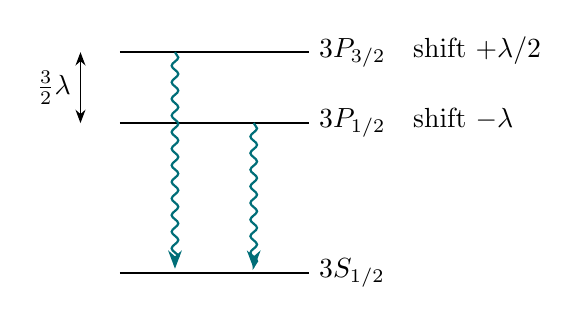
\begin{tikzpicture}[>=Stealth,scale=1.0]
\draw[thick] (0,2.8)--(2.4,2.8) node[right]{$3P_{3/2}$\quad shift $+\lambda/2$};
\draw[thick] (0,1.9)--(2.4,1.9) node[right]{$3P_{1/2}$\quad shift $-\lambda$};
\draw[thick] (0,0)--(2.4,0) node[right]{$3S_{1/2}$};
\draw[decorate,decoration={snake,amplitude=1.2pt,segment length=6pt},->,secondary,thick] (0.7,2.8)--(0.7,0.05);
\draw[decorate,decoration={snake,amplitude=1.2pt,segment length=6pt},->,secondary,thick] (1.7,1.9)--(1.7,0.05);
\draw[<->] (-0.5,1.9)--(-0.5,2.8) node[midway,left]{$\tfrac32\lambda$};
\end{tikzpicture}
\end{center}
The two transitions $3P_{3/2}\to3S_{1/2}$ and $3P_{1/2}\to3S_{1/2}$ give the \textbf{two lines of sodium} (the yellow doublet).

\subsection{Spectroscopic Notation}
The level label is $n\,L_j$: $n$ the principal quantum number, $L$ a letter for the orbital angular momentum, and $j$ the total angular momentum:
\[
\ell=0\Rightarrow S,\qquad \ell=1\Rightarrow P,\qquad \ell=2\Rightarrow D,\ \dots
\]

\textbf{*** Study Note:} The full term symbol is $n^{2s+1}L_j$; for a single electron the multiplicity superscript $2s+1=2$ is conventionally omitted when $s=\tfrac12$ is understood. The doublet in the name of the effect is exactly the $j=\ell\pm\tfrac12$ splitting.

\subsection{Magnetic Field: Two Limits}
The magnetic moments from the orbital motion and from the intrinsic spin are
\[
\vec\mu_L=-\frac{e\hbar}{2mc}\,\frac{\hat{\vec L}}\hbar,\qquad \vec\mu_S=-\frac{e\hbar}{2mc}\,\frac{2\hat{\vec S}}\hbar ,
\]
(the factor 2 in the spin moment is the electron $g$-factor). Apply $\vec B=B\hat e_z$. The effective Hamiltonian becomes
\[
\hat H_{\mathrm{eff}}=-\frac{\hbar^2}{2m}\nabla^2+V(r)+\lambda\,\hat{\vec L}\cdot\hat{\vec S}+\frac{e\hbar}{2mc}B\,\big(\hat L_z+2\hat S_z\big),
\]
where, as in the notes, $\hat L_z,\hat S_z$ in the last term are measured in units of $\hbar$. Neither of the two bases commutes with this Hamiltonian in general, so two limits are considered.

\begin{thm}{Zeeman and Paschen-Back Limits}
\textbf{(i) Zeeman limit} (spin-orbit coupling strong): $\ \lambda\hat{\vec L}\cdot\hat{\vec S}\gg\dfrac{e\hbar B}{2mc}(\hat L_z+2\hat S_z)$. Use the coupled basis $|j,m,\ell,s\rangle$; the field is a small perturbation.

\textbf{(ii) Paschen-Back limit} (spin-orbit coupling weak): $\ \lambda\hat{\vec L}\cdot\hat{\vec S}\ll\dfrac{e\hbar B}{2mc}(\hat L_z+2\hat S_z)$. Use the uncoupled basis $|\ell,s,m_\ell,m_s\rangle$; the spin-orbit term is a small perturbation.
\end{thm}

\textbf{*** Complete Solution:} In the Paschen-Back limit, the zeroth-order energy shift from the field is $\dfrac{e\hbar B}{2mc}(m_\ell+2m_s)$. The first-order spin-orbit correction is the expectation value of $\lambda\hat{\vec L}\cdot\hat{\vec S}=\lambda\big(\hat L_z\hat S_z+\tfrac12(\hat L_+\hat S_-+\hat L_-\hat S_+)\big)$, where only the diagonal term $\lambda\hbar^2m_\ell m_s$ contributes. In the Zeeman limit the field splits each $j$-level into $2j+1$ sublevels, $\Delta E=g_J\,\mu_BBm$.

\textbf{*** Exam Tip:} A common question is \emph{which basis, and why}. The answer is a comparison of the two terms: whichever of the two perturbation terms dominates picks the basis in which it is diagonal, and the weaker term is treated as a perturbation.

%==============================================================================
\section{Central Potentials}
\label{sy:sec:central}
%==============================================================================

\subsection{Separation of the Schr\"odinger Equation}
For a central potential $V(\vec r)=V(r)$ the time-independent Schr\"odinger equation is
\[
\Big(-\frac{\hbar^2}{2m}\nabla^2+V(r)\Big)\psi(\vec r)=E\,\psi(\vec r).
\]
In spherical coordinates the Laplacian splits into a radial part and an angular part, giving
\[
\Big[-\frac{\hbar^2}{2m}\,\frac1r\frac{\partial^2}{\partial r^2}\,r+\frac{\hat L^2}{2mr^2}+V(r)\Big]\psi(\vec r)=E\,\psi(\vec r).
\]
The potential depends on $r$ only, so the Hamiltonian is rotation invariant and $[\hat H,\hat L^2]=0=[\hat H,\hat L_z]$ (Section~\ref{sy:sec:rot}). Therefore the eigenfunctions are simultaneous eigenfunctions of $\hat H,\hat L^2,\hat L_z$:
\[
\psi(\vec r)=\langle\vec r|n,\ell,m\rangle=R_{n\ell}(r)\,Y_{\ell m}(\theta,\phi).
\]

\subsection{The Radial Equation}
Substitute this form into the equation and use $\hat L^2Y_{\ell m}=\hbar^2\ell(\ell+1)Y_{\ell m}$. The angular function factors out:
\[
Y_{\ell m}\Big[-\frac{\hbar^2}{2m}\frac1r\frac{d^2}{dr^2}\big(rR_{n\ell}\big)+\big(V(r)-E\big)R_{n\ell}+\frac{\hbar^2\ell(\ell+1)}{2mr^2}R_{n\ell}\Big]=0 .
\]
Multiplying by $r$:
\[
-\frac{\hbar^2}{2m}\frac{d^2}{dr^2}\big(rR_{n\ell}\big)+\Big[V(r)+\frac{\ell(\ell+1)\hbar^2}{2mr^2}\Big]rR_{n\ell}=E\,rR_{n\ell}.
\]
Choose
\[
u_{n\ell}(r)=r\,R_{n\ell}(r),\qquad V_{\mathrm{eff}}(r)=V(r)+\frac{\ell(\ell+1)\hbar^2}{2mr^2}.
\]

\begin{thm}{Radial Equation}
\[
-\frac{\hbar^2}{2m}\frac{d^2u_{n\ell}}{dr^2}+V_{\mathrm{eff}}(r)\,u_{n\ell}(r)=E_n\,u_{n\ell}(r),\qquad \lim_{r\to0}u_{n\ell}(r)=\lim_{r\to0}rR_{n\ell}(r)=0 .
\]
\end{thm}

This is a one-dimensional Schr\"odinger equation on the half line $r>0$ in the effective potential $V_{\mathrm{eff}}$, with the condition $u(0)=0$ imposed because $R_{n\ell}$ must stay finite at the origin.

\textbf{*** Intuition:} The extra term $\ell(\ell+1)\hbar^2/2mr^2$ is the \emph{centrifugal barrier}. It repels the particle from the origin, more strongly for larger $\ell$, so higher-$\ell$ states sit farther out.

\begin{center}
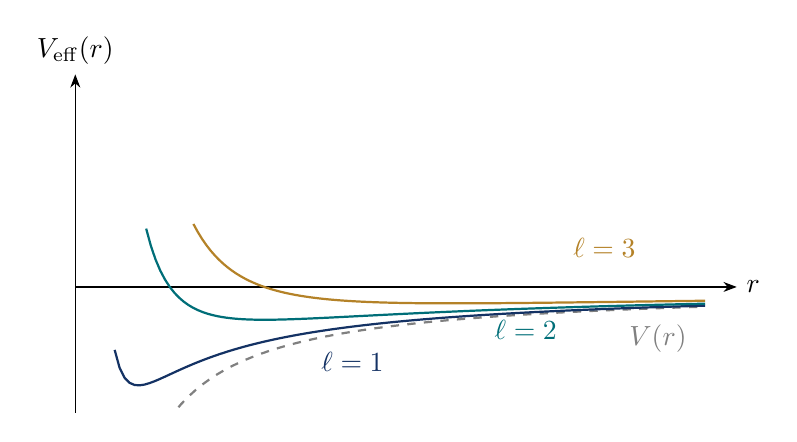
\begin{tikzpicture}[>=Stealth,xscale=1.0,yscale=1.0,
  declare function={veff(\x,\l)=-2/\x+0.4*\l*(\l+1)/(\x*\x);}]
\draw[->] (0,0)--(8.4,0) node[right]{$r$};
\draw[->] (0,-1.6)--(0,2.7) node[above]{$V_{\mathrm{eff}}(r)$};
\begin{scope}
\clip (0,-1.6) rectangle (8.2,2.6);
\draw[thick,gray,dashed,domain=0.7:8,samples=80] plot(\x,{-2/\x});
\draw[thick,primary,domain=0.5:8,samples=120] plot(\x,{veff(\x,1)});
\draw[thick,secondary,domain=0.9:8,samples=120] plot(\x,{veff(\x,2)});
\draw[thick,exframe,domain=1.5:8,samples=120] plot(\x,{veff(\x,3)});
\end{scope}
\node[gray,below] at (7.4,-0.35) {$V(r)$};
\node[primary,right] at (3.0,-0.95) {$\ell=1$};
\node[secondary,right] at (5.2,-0.55) {$\ell=2$};
\node[exframe,above right] at (6.2,0.25) {$\ell=3$};
\end{tikzpicture}
\end{center}
As $\ell$ increases the effective potential becomes higher and its minimum moves outward, away from the origin.

\textbf{*** Study Note:} The notebook's caption for this figure says the minima shift ``farther to the origin''. From $V_{\mathrm{eff}}=V+\ell(\ell+1)\hbar^2/2mr^2$ the barrier grows with $\ell$, so the minimum moves \emph{away from} the origin (to larger $r$), which is also what the sketch shows, with the $\ell=3$ curve having its minimum farthest to the right.

\textbf{*** Study Note:} The energy $E_n$ does not depend on $m$ (it appears nowhere in the radial equation), so every level is at least $(2\ell+1)$-fold degenerate. For potentials such as the Coulomb one there is additional $\ell$-degeneracy, but that is not generic.

\begin{prob}{Free Particle Check, $V=0$, $\ell=0$}
\textbf{*** Complete Solution:} The radial equation is $-\frac{\hbar^2}{2m}u''=Eu$ with $u(0)=0$, giving $u(r)=A\sin kr$ with $k=\sqrt{2mE}/\hbar$. Then $R_{k0}=A\sin(kr)/r$, which is finite at the origin, and $\psi=R\,Y_{00}$. The alternative $\cos kr$ is excluded by $u(0)=0$ (it would give $R\sim1/r$).
\end{prob}


%%% PART 3
\partheading{Tensor Operators, Wigner-Eckart and the Projection Theorem}{This part covers how operators transform under rotations: scalar and vector operators, Cartesian tensors and their decomposition into irreducible pieces, irreducible spherical tensor operators and their commutation relations with $\hat{\vec J}$, the Wigner-Eckart theorem (with the dipole matrix element and the selection rules as the main application), and the projection theorem (with the spin expectation value and the Land\'e factor as applications). It continues directly from Part~II on angular momentum and Clebsch-Gordan coefficients.}




%==============================================================================
\section{Scalar and Vector Operators}
\label{to:sec:scalvec}
%==============================================================================

\subsection{How an Operator Transforms Under a Rotation}
For an infinitesimal rotation through $\delta\theta$ about the axis $\hat n$, the rotation operator is
\[
\hat U_{\hat n}(\delta\theta)=\mathbb 1-\frac i\hbar\,\delta\theta\ \hat n\cdot\hat{\vec J}.
\]
A state transforms as $|\psi'\rangle=\hat U|\psi\rangle$, and an operator transforms as
\begin{align*}
\hat A'&=\hat U^\dagger\hat A\,\hat U=\Big(\mathbb 1+\frac i\hbar\,\delta\theta\ \hat n\cdot\hat{\vec J}\Big)\hat A\Big(\mathbb 1-\frac i\hbar\,\delta\theta\ \hat n\cdot\hat{\vec J}\Big)\\
&=\hat A-\frac i\hbar\,\delta\theta\,\big[\hat A,\hat n\cdot\hat{\vec J}\,\big]+O(\delta\theta^2).
\end{align*}
This one formula fixes what ``scalar'', ``vector'' and ``tensor'' mean quantum mechanically: each is defined by how $\hat A'$ must relate to $\hat A$.

\subsection{Scalar Operators}
A scalar is unchanged by a rotation, $\hat A'=\hat A$. Comparing with the expansion above:

\begin{thm}{Scalar Operator}
\[
\hat A'=\hat A\quad\Longrightarrow\quad\big[\hat A,\hat n\cdot\hat{\vec J}\,\big]=0\ \ \text{for every }\hat n,\qquad\text{i.e.}\quad[\hat A,\hat{\vec J}\,]=0 .
\]
\end{thm}

\textbf{*** Study Note:} Examples are $\hat J^2$, $\hat r^2$, $\hat p^2$, $\hat{\vec L}\cdot\hat{\vec S}$ and the Hamiltonian of a central potential. A rotation-invariant Hamiltonian is exactly a scalar operator, which is the statement $[\hat H,\hat{\vec J}\,]=0$ of Part~II.

\subsection{Vector Operators}
A vector operator transforms like the position vector. For $\vec r$ under an infinitesimal rotation,
\[
\vec r\,'=\vec r+\delta\theta\,(\hat n\times\vec r\,),
\]
so for a vector operator
\[
\hat{\vec A}\,'=\hat{\vec A}+\delta\theta\,(\hat n\times\hat{\vec A}).\tag{II}
\]
Equating this with the general rule, labelled (I), $\hat{\vec A}\,'=\hat{\vec A}-\frac i\hbar\delta\theta[\hat{\vec A},\hat n\cdot\hat{\vec J}\,]$:
\[
\hat{\vec A}-\frac i\hbar\,\delta\theta\,\big[\hat{\vec A},\hat n\cdot\hat{\vec J}\,\big]=\hat{\vec A}+\delta\theta\,(\hat n\times\hat{\vec A}),
\qquad\text{so}\qquad
\big[\hat{\vec A},\hat n\cdot\hat{\vec J}\,\big]=i\hbar\,(\hat n\times\hat{\vec A}).
\]
In components, $(\hat n\times\hat{\vec A})_\ell=\epsilon_{\ell mn}\,n_m\hat A_n$.

\begin{thm}{Vector Operator}
\[
\big[\hat A_\ell,\hat n\cdot\hat{\vec J}\,\big]=i\hbar\,\epsilon_{\ell mn}\,n_m\hat A_n .
\]
\end{thm}

\subsection{The Cartesian Commutation Relations}
Take $\ell=1$. The left side is $n_1[\hat A_1,\hat J_1]+n_2[\hat A_1,\hat J_2]+n_3[\hat A_1,\hat J_3]$, and the right side is
\[
i\hbar\,\epsilon_{1mn}n_m\hat A_n=i\hbar\,\epsilon_{123}n_2\hat A_3+i\hbar\,\epsilon_{132}n_3\hat A_2=i\hbar\,n_2\hat A_3-i\hbar\,n_3\hat A_2 .
\]
The vector $\hat n$ is arbitrary, so equating the coefficients of $n_1,n_2,n_3$ and then cycling the indices gives:
\begin{thm}{Defining Commutators of a Vector Operator}
\begin{gather*}
[\hat A_x,\hat J_x]=[\hat A_y,\hat J_y]=[\hat A_z,\hat J_z]=0,\\
[\hat A_x,\hat J_y]=i\hbar\hat A_z,\qquad[\hat A_y,\hat J_z]=i\hbar\hat A_x,\qquad[\hat A_z,\hat J_x]=i\hbar\hat A_y .
\end{gather*}
\end{thm}

\textbf{Check with $\hat{\vec A}=\hat{\vec J}$:} $[\hat J_1,\hat J_2]=i\hbar\hat J_3$ and $[\hat J_1,\hat J_3]=-i\hbar\hat J_2$. This reproduces the angular momentum algebra, so $\hat{\vec J}$ itself is a vector operator. This is a consistency check on the definition: the algebra derived from rotations in Part~II is the statement that the generators transform like a vector.

\subsection{Spherical Components of a Vector Operator}
Define $\hat A_\pm=\hat A_x\pm i\hat A_y$. From the identities,
\[
[\hat J_x,\hat A_\pm]=[\hat J_x,\hat A_x]\pm i[\hat J_x,\hat A_y]=\pm i\,(i\hbar\hat A_z)=\mp\hbar\hat A_z .
\]

\begin{thm}{Spherical Components}
\[
\hat A_{\pm1}=\mp\frac1{\sqrt2}\big(\hat A_x\pm i\hat A_y\big),\qquad \hat A_0=\hat A_z .
\]
\end{thm}

For the position vector $\vec r=r_1\hat e_1+r_2\hat e_2+r_3\hat e_3$ with $r_1=x=r\sin\theta\cos\phi$, $r_2=y=r\sin\theta\sin\phi$, $r_3=z=r\cos\theta$, the spherical components are proportional to the $\ell=1$ spherical harmonics:
\begin{align*}
r^{(1)}_{+1}&=-\tfrac1{\sqrt2}(x+iy)=-\tfrac1{\sqrt2}\,r\sin\theta\,e^{i\phi}=r\sqrt{\tfrac{4\pi}3}\,Y^{(1)}_{+1}(\theta,\phi),\\
r^{(1)}_{-1}&=\ \ \tfrac1{\sqrt2}(x-iy)=\ \ \tfrac1{\sqrt2}\,r\sin\theta\,e^{-i\phi}=r\sqrt{\tfrac{4\pi}3}\,Y^{(1)}_{-1}(\theta,\phi),\\
r^{(1)}_{0}&=z=r\cos\theta=r\sqrt{\tfrac{4\pi}3}\,Y^{(1)}_{0}(\theta,\phi).
\end{align*}
Here $r^{(1)}_q$ with $q=-1,0,1$ is the notation used from now on, where the superscript $(1)$ is the rank and the subscript $q$ labels the component. Here $Y^{(1)}_q\equiv Y_{1q}$.

\textbf{*** Verification:} Using $Y_{1,\pm1}=\mp\sqrt{3/8\pi}\sin\theta\,e^{\pm i\phi}$ and $Y_{10}=\sqrt{3/4\pi}\cos\theta$ from the earlier notes, $r\sqrt{4\pi/3}\,Y_{1,\pm1}=\mp\tfrac r{\sqrt2}\sin\theta\,e^{\pm i\phi}$, in agreement with the first two lines.

\textbf{*** Complete Solution:} The spherical components have simple commutators with $\hat J_z$. From the identities, $[\hat J_z,\hat A_x]=i\hbar\hat A_y$ and $[\hat J_z,\hat A_y]=-i\hbar\hat A_x$, so
\[
[\hat J_z,\hat A_\pm]=i\hbar\hat A_y\pm i(-i\hbar\hat A_x)=\pm\hbar\big(\hat A_x\pm i\hat A_y\big)=\pm\hbar\hat A_\pm,\qquad[\hat J_z,\hat A_0]=0 .
\]
Hence $[\hat J_z,\hat A_q]=\hbar q\,\hat A_q$ for $q=-1,0,1$. Similarly $[\hat J_+,\hat A_z]=[\hat J_x,\hat A_z]+i[\hat J_y,\hat A_z]=-i\hbar\hat A_y+i(i\hbar\hat A_x)=-\hbar\hat A_+=\sqrt2\,\hbar\,\hat A_{+1}$. These are exactly the pattern that defines an irreducible tensor of rank one (Section~\ref{to:sec:irr}).

%==============================================================================
\section{Cartesian Tensors: Reducible and Irreducible}
\label{to:sec:cart}
%==============================================================================

\subsection{Scalars, Vectors and Tensors Under a Rotation Matrix}
Let $R_{ia}$ be the rotation matrix, with $R^TR=\mathbb 1$. Under a rotation of the axes:
\begin{itemize}
\item \textbf{Scalars} are invariant.
\item \textbf{Vectors}: $v_i'=\sum_aR_{ia}v_a$.
\item \textbf{Tensors}: $T'_{ij}=\sum_{a,b}R_{ia}R_{jb}T_{ab}$ (rank 2), $\ T'_{ijk}=\sum_{a,b,c}R_{ia}R_{jb}R_{kc}T_{abc}$ (rank 3), and so on.
\end{itemize}

\textbf{Example: the dot product is a scalar.} Let $\varphi=v_iw_i$. Then
\begin{align*}
\varphi'&=v_i'w_i'=R_{ia}R_{ib}\,v_aw_b=R^T_{ai}R_{ib}\,v_aw_b=(R^TR)_{ab}\,v_aw_b\\
&=\delta_{ab}\,v_aw_b=v_aw_a=\varphi ,
\end{align*}
using $R^TR=\mathbb 1$. The quantity $\varphi$ remains invariant.

Now take the product $T_{ij}=v_iw_j$, which has nine components. It transforms as a rank-2 tensor:
\[
T'_{ij}=v_i'w_j'=R_{ia}R_{jb}\,v_aw_b=R_{ia}R_{jb}\,T_{ab}.
\]

\subsection{Reducible Tensors: Decomposition of Rank 2}
A Cartesian tensor of rank 2 has $3^2=9$ components but can be split into three pieces that never mix under rotation:
\begin{thm}{Decomposition of a Rank-2 Tensor}
\begin{align*}
T^{(0)}_{ij}&=\tfrac13\,\delta_{ij}\sum_{k=1}^{3}T_{kk}&&\to\ 1\ \text{component (scalar part)},\\
T^{(1)}_{ij}&=\tfrac12\,(T_{ij}-T_{ji})&&\to\ 3\ \text{components (vector part, antisymmetric)},\\
T^{(2)}_{ij}&=\tfrac12\,(T_{ij}+T_{ji})-T^{(0)}_{ij}&&\to\ 5\ \text{components (symmetric, traceless)}.
\end{align*}
Any rank-2 tensor is the sum $T=T^{(0)}+T^{(1)}+T^{(2)}$, and $1+3+5=9$.
\end{thm}

The antisymmetric part has $3$ independent components (the diagonal vanishes and $T_{ji}=-T_{ij}$, so only $i<j$ pairs count). The symmetric part has $6$ independent components, and removing the trace (one condition) leaves $5$.

\textbf{*** Complete Solution (example $T_{ij}=v_iw_j$):} The three pieces are
\begin{align*}
T^{(0)}_{ij}&=\tfrac13\,\delta_{ij}\,\vec v\cdot\vec w,\\
T^{(1)}_{ij}&=\tfrac12\,(v_iw_j-v_jw_i)\ \leftrightarrow\ \tfrac12\,(\vec v\times\vec w\,)_k,\\
T^{(2)}_{ij}&=\tfrac12\,(v_iw_j+v_jw_i)-\tfrac13\,\delta_{ij}\,\vec v\cdot\vec w .
\end{align*}
So the nine products $v_iw_j$ split into the dot product (a scalar), the cross product (a vector) and a symmetric traceless remainder with five components.

\subsection{Irreducible Tensors}
A Cartesian tensor of rank $k$ can be decomposed into tensors of lower rank, each a linear combination of the $3^k$ components. The pieces that cannot be reduced any further are the irreducible parts.

\begin{thm}{Irreducible Tensor of Rank $k$}
A set of $(2k+1)$ components that behaves as a rank-$k$ tensor and cannot be reduced is an \emph{irreducible tensor of rank $k$}. The $(2k+1)$ components are symmetric and traceless.
\end{thm}

The decomposition above is an example: $T^{(0)},T^{(1)},T^{(2)}$ are irreducible tensors of rank $0,1,2$ with $1,3,5$ components.

\textbf{*** Intuition:} Irreducibility means the pieces carry independent sets of states under rotation, exactly as the $2j+1$ states $|j,m\rangle$ of a fixed $j$ never mix with those of a different $j$. That is why irreducible tensors can be matched with angular momentum states.

\subsection{Irreducible Spherical Tensors}
\begin{thm}{Definition (Irreducible Spherical Tensor)}
An irreducible spherical tensor of rank $k$ ($k$ an integer) is a set of $(2k+1)$ operators $\hat T^{(k)}_q$, $q=-k,\dots,0,\dots,k$, which transform under a rotation of the axes in the same way as the angular momentum states $|k,q\rangle$.
\end{thm}

For $k=1$:
\[
\hat T^{(1)}_{\pm1}=\mp\frac1{\sqrt2}\big(\hat A_x\pm i\hat A_y\big),\qquad\hat T^{(1)}_0=\hat A_z ,
\]
which are exactly the spherical components of a vector operator from Section~\ref{to:sec:scalvec}. A scalar is $k=0$ (one component, $q=0$) and a vector is $k=1$.

\textbf{*** Study Note:} A rank-2 irreducible tensor has five components $T^{(2)}_q$, $q=-2,\dots,2$. If $\hat A,\hat B$ are two vector operators, the five combinations $\hat A_{+1}\hat B_{+1}$, $\tfrac1{\sqrt2}(\hat A_{+1}\hat B_0+\hat A_0\hat B_{+1})$, $\tfrac1{\sqrt6}(\hat A_{+1}\hat B_{-1}+2\hat A_0\hat B_0+\hat A_{-1}\hat B_{+1})$, $\tfrac1{\sqrt2}(\hat A_{-1}\hat B_0+\hat A_0\hat B_{-1})$, $\hat A_{-1}\hat B_{-1}$ form $\hat T^{(2)}_{q}$ for $q=2,1,0,-1,-2$. These are the Clebsch-Gordan combinations of two $k=1$ objects, as for two spin-1 particles coupled to total spin 2.

%==============================================================================
\section{Irreducible Tensor Operators and Their Commutation Relations}
\label{to:sec:irr}
%==============================================================================

\subsection{Definition}
An irreducible tensor operator is written $\hat T^{(k)}_q$, where $k$ is the \textbf{rank} and $q$ labels the $2k+1$ \textbf{components}, $q=-k,\dots,k$. For $k=1$, $q=-1,0,1$, and
\[
\hat T^{(1)}_{\pm1}=\mp\frac1{\sqrt2}\big(\hat A_x\pm i\hat A_y\big),\qquad \hat T^{(1)}_0=\hat A_z .
\]

\subsection{The Commutation Relations}
Requiring $\hat T^{(k)}_q$ to transform under rotations like the angular momentum states $|k,q\rangle$ is equivalent to the following commutators with $\hat{\vec J}$.

\begin{thm}{Defining Relations of an Irreducible Tensor Operator}
\begin{align*}
[\hat J_z,\hat T^{(k)}_q]&=\hbar q\,\hat T^{(k)}_q,\tag{I}\\
[\hat J_\pm,\hat T^{(k)}_q]&=\hbar\sqrt{(k\mp q)(k\pm q+1)}\ \hat T^{(k)}_{q\pm1},\tag{II}\\
\sum_i\big[\hat J_i,[\hat J_i,\hat T^{(k)}_q]\big]&=\hbar^2k(k+1)\,\hat T^{(k)}_q,
\end{align*}
where $\hat J_\pm=\hat J_x\pm i\hat J_y$.
\end{thm}

\textbf{*** Intuition:} Compare with $\hat J_z|k,q\rangle=\hbar q|k,q\rangle$ and $\hat J_\pm|k,q\rangle=\hbar\sqrt{(k\mp q)(k\pm q+1)}\,|k,q\pm1\rangle$. The operator $[\hat J_z,\,\cdot\,]$ acts on $\hat T^{(k)}_q$ as $\hat J_z$ acts on $|k,q\rangle$, and the double commutator is the analogue of $\hat J^2$. So $\hat T^{(k)}_q$ ``behaves as an angular momentum state'' under the adjoint action.

\textbf{*** Verification (rank 1):} The relations (I) and (II) agree with the vector results of Section~\ref{to:sec:scalvec}: $[\hat J_z,\hat A_q]=\hbar q\hat A_q$, and $[\hat J_+,\hat A_0]=\sqrt2\,\hbar\hat A_{+1}$, which is (II) with $k=1$, $q=0$, since $\sqrt{(1-0)(1+0+1)}=\sqrt2$.

\subsection{Selection Rule on \texorpdfstring{$m$}{m}}
Take the matrix element of relation (I) between angular momentum states:
\begin{align*}
\langle j',m'|[\hat J_z,\hat T^{(k)}_q]|j,m\rangle&=\langle j',m'|\hat J_z\hat T^{(k)}_q-\hat T^{(k)}_q\hat J_z|j,m\rangle=\hbar(m'-m)\langle j',m'|\hat T^{(k)}_q|j,m\rangle,\\
&=\hbar q\,\langle j',m'|\hat T^{(k)}_q|j,m\rangle .
\end{align*}
Therefore $(m'-m-q)\langle j',m'|\hat T^{(k)}_q|j,m\rangle=0$.

\begin{thm}{$m$ Selection Rule}
\[
\langle j',m'|\hat T^{(k)}_q|j,m\rangle\neq0\quad\text{only if}\quad m'=m+q .
\]
\end{thm}

\textbf{*** Intuition:} The operator $\hat T^{(k)}_q$ carries $q$ units of angular momentum about $z$. Acting on a state with $J_z=\hbar m$ it creates a state with $J_z=\hbar(m+q)$.

\subsection{A Recursion Relation for the Matrix Elements}
Now take the matrix element of (II) with the raising operator:
\[
\langle j',m'|[\hat J_+,\hat T^{(k)}_q]|j,m\rangle=\hbar\sqrt{(k-q)(k+q+1)}\ \langle j',m'|\hat T^{(k)}_{q+1}|j,m\rangle .
\]
The left side is $\langle j',m'|\hat J_+\hat T^{(k)}_q-\hat T^{(k)}_q\hat J_+|j,m\rangle$. Use, for the first term,
\[
\langle j',m'|\hat J_+=\big[\hat J_-|j',m'\rangle\big]^\dagger=\hbar\sqrt{(j'+m')(j'-m'+1)}\,\langle j',m'-1|,
\]
and, for the second term,
\[
\hat J_+|j,m\rangle=\hbar\sqrt{(j-m)(j+m+1)}\,|j,m+1\rangle .
\]
Cancelling the common $\hbar$:

\begin{thm}{Recursion for Matrix Elements of $\hat T^{(k)}_q$}
\begin{align*}
\sqrt{(j'+m')(j'-m'+1)}\ \langle j',m'-1|\hat T^{(k)}_q|j,m\rangle&-\sqrt{(j-m)(j+m+1)}\ \langle j',m'|\hat T^{(k)}_q|j,m+1\rangle\\
&=\sqrt{(k-q)(k+q+1)}\ \langle j',m'|\hat T^{(k)}_{q+1}|j,m\rangle .\tag{A}
\end{align*}
\end{thm}

This linear relation connects matrix elements with different values of $m,q,m'$. The next section shows that the Clebsch-Gordan coefficients satisfy the \emph{same} relation, which forces the matrix elements to be proportional to them.

%==============================================================================
\section{The Wigner-Eckart Theorem}
\label{to:sec:we}
%==============================================================================

\subsection{Idea of the Derivation}
The matrix elements $\langle j',m'|\hat T^{(k)}_q|j,m\rangle$ obey the linear recursion (A) of Section~\ref{to:sec:irr}. The Clebsch-Gordan coefficients for coupling the angular momenta $j$ and $k$ into $j'$ obey a recursion of the same form. If two sets of numbers satisfy the same homogeneous recursion, they are proportional. The proportionality constant cannot depend on $m,q,m'$, which is the content of the theorem.

\subsection{Coupling \texorpdfstring{$j$}{j} and \texorpdfstring{$k$}{k}}
Consider the product states $|j,m,k,q\rangle=|j,m\rangle\otimes|k,q\rangle$, and couple $j$ with $k$ to a total $j'$ (any value allowed by the triangle rule $|j-k|\le j'\le j+k$). The conservation $m'=m+q$ holds, and
\[
|j',m'\rangle=\sum_{m,q}\langle j,m,k,q|j',m'\rangle\,|j,m,k,q\rangle\equiv\sum_{m,q}C(j,k,j'\,|\,m,q,m')\,|j,m,k,q\rangle .
\]
Apply the total lowering operator $\hat J_-'=\hat J_-+\hat K_-$, where $\hat K_-$ acts on the $|k,q\rangle$ part. The left side is
\begin{align*}
\hat J_-'|j',m'\rangle&=\hbar\sqrt{(j'+m')(j'-m'+1)}\,|j',m'-1\rangle\\
&=\hbar\sqrt{(j'+m')(j'-m'+1)}\sum_{m,q}C(jkj'|m,q,m'-1)\,|j,m,k,q\rangle ,
\end{align*}
and the right side is
\[
\sum_{m,q}C(jkj'|m,q,m')\Big[\hbar\sqrt{(j+m)(j-m+1)}\,|j,m-1,k,q\rangle+\hbar\sqrt{(k+q)(k-q+1)}\,|j,m,k,q-1\rangle\Big].
\]
In the first term replace $m\to m+1$ and in the second $q\to q+1$, so that all kets read $|j,m,k,q\rangle$ (labelled (B) and (B$'$) in the notes). The kets are linearly independent, so their coefficients must match:

\begin{thm}{Recursion for the Clebsch-Gordan Coefficients}
\begin{align*}
\sqrt{(j'+m')(j'-m'+1)}\ C(jkj'|m,q,m'-1)&=\sqrt{(j+m+1)(j-m)}\ C(jkj'|m+1,q,m')\\
&\quad+\sqrt{(k+q+1)(k-q)}\ C(jkj'|m,q+1,m').\tag{C}
\end{align*}
\end{thm}

\subsection{Comparison with the Tensor Recursion}
Place (A) and (C) side by side. They are identical in form under the correspondence
\begin{gather*}
\langle j',m'-1|\hat T^{(k)}_q|j,m\rangle\leftrightarrow C(jkj'|m,q,m'-1),\\
\langle j',m'|\hat T^{(k)}_q|j,m+1\rangle\leftrightarrow C(jkj'|m+1,q,m'),\\
\langle j',m'|\hat T^{(k)}_{q+1}|j,m\rangle\leftrightarrow C(jkj'|m,q+1,m').
\end{gather*}
Therefore
\[
\langle j',m'|\hat T^{(k)}_q|j,m\rangle\ \propto\ C(jkj'|m,q,m').
\]

\textbf{*** Study Note:} The notebook states ``we can take $j'=j+k$'' before building $|j',m'\rangle$. Nothing in the argument depends on that choice: relation (C) holds for each allowed $j'$ separately, and the proportionality constant is allowed to depend on $j,j',k$ (and on any other labels such as $n$), but not on $m,q,m'$.

\begin{thm}{Wigner-Eckart Theorem}
\[
\boxed{\ \langle j',m'|\hat T^{(k)}_q|j,m\rangle=\langle j'\|\hat T^{(k)}\|j\rangle\ \cdot\ C(jkj'|m,q,m')\ }
\]
The first factor, the \textbf{reduced matrix element}, is the \emph{dynamical factor}: it depends on the operator and the physical system but not on $m,q,m'$. The second factor, the Clebsch-Gordan coefficient, is the \emph{geometric factor}: it depends only on the rotational symmetry.
\end{thm}

\subsection{Notations}
The Clebsch-Gordan coefficient appears in the notes in several forms,
\[
C(jkj'|m,q,m')\ \equiv\ C^{\,j'm'}_{\,jm,\,kq}\ \equiv\ \begin{pmatrix}j&k&j'\\m&q&m'\end{pmatrix}.
\]

\textbf{*** Study Note:} The last symbol (the Wigner $3j$ symbol) is closely related to the Clebsch-Gordan coefficient but not identical: it differs by a normalisation factor $\sqrt{2j'+1}$ and a phase, so reduced matrix elements quoted with a $3j$ symbol differ from those used here by that factor. Always check which convention a formula uses.

\subsection{Consequences}
\begin{enumerate}[leftmargin=2em,itemsep=2pt]
\item \textbf{Magnetic selection rule:} $m'=m+q$.
\item \textbf{Triangle selection rule:} $\langle j',m'|\hat T^{(k)}_q|j,m\rangle=0$ unless $|j-k|\le j'\le j+k$, since otherwise the Clebsch-Gordan coefficient vanishes.
\item \textbf{Fixed ratios:} within a pair of multiplets $(j,j')$, the ratio of any two matrix elements of $\hat T^{(k)}_q$ equals the ratio of two Clebsch-Gordan coefficients, regardless of the physics inside the reduced element.
\end{enumerate}

\subsection{Scalar Operators}
For a scalar operator $k=0$ and $q=0$. The coupling $j\otimes0$ gives only $j'=j$, $m'=m$, so
\[
C(j,0,j'|m,0,m')=\delta_{jj'}\delta_{mm'},
\]
and
\[
\langle j',m'|\hat T^{(0)}_0|j,m\rangle=\delta_{jj'}\delta_{mm'}\,\langle j'\|\hat T^{(0)}\|j\rangle .
\]
\begin{thm}{Scalar Operator Matrix Elements}
A scalar operator is diagonal in $j$ and $m$, and its diagonal element does not depend on $m$.
\end{thm}

This agrees with Section~\ref{to:sec:scalvec}: $[\hat A,\hat{\vec J}\,]=0$ means $\hat A$ cannot change $j$ or $m$.

%==============================================================================
\section{Application: Dipole Matrix Elements and Selection Rules}
\label{to:sec:dipole}
%==============================================================================

\subsection{The \texorpdfstring{$2s\to2p$}{2s to 2p} Dipole Matrix Element}
Take hydrogen-like states $|n,\ell,m\rangle$. The dipole operator is a rank-1 tensor operator, $\hat r^{(1)}_q$. Consider the $2s\to2p$ transition: the dipole term contributes to the transition if
\[
\langle n'=2,\ell'=1,m'=0|\,\hat r^{(1)}_0\,|n=2,\ell=0,m=0\rangle\neq0 .
\]
By the Wigner-Eckart theorem with $\ell=0$, $m=0$, $k=1$, $q=0$, $\ell'=1$, $m'=0$:
\[
\langle\ell',m'|\hat r^{(1)}_0|\ell=0,m=0\rangle=C^{\ell'm'}_{\ell m,kq}\,\langle\ell'\|\hat r^{(1)}\|\ell\rangle=C^{10}_{00,10}\,\langle1\|\hat r^{(1)}\|0\rangle=\langle1\|\hat r^{(1)}\|0\rangle,
\]
since coupling $\ell=0$ with $k=1$ gives $C^{10}_{00,10}=1$. The reduced element is built from the radial integral of the hydrogen functions
\[
R_{2s}=\frac1{\sqrt{2a_0^3}}\Big(1-\frac r{2a_0}\Big)e^{-r/2a_0},\qquad R_{2p}=\frac1{\sqrt{24a_0^3}}\,\frac r{a_0}\,e^{-r/2a_0}.
\]

\textbf{*** Complete Solution:} The radial integral, with $x=r/a_0$, is
\begin{align*}
\int_0^\infty R_{2p}\,r\,R_{2s}\,r^2\,dr&=\frac{a_0}{\sqrt{48}}\int_0^\infty x^4\Big(1-\frac x2\Big)e^{-x}\,dx=\frac{a_0}{\sqrt{48}}\big(4!-\tfrac12\,5!\big)\\
&=-\frac{36}{\sqrt{48}}\,a_0=-3\sqrt3\,a_0\approx-5.196\,a_0 .
\end{align*}
The angular part supplies a factor $\int Y_{10}^*\cos\theta\,Y_{00}\,d\Omega=1/\sqrt3$, so the full matrix element is
\[
\langle2,1,0|\,z\,|2,0,0\rangle=\langle1\|\hat r^{(1)}\|0\rangle=-\frac{3\sqrt3}{\sqrt3}\,a_0=-3\,a_0 .
\]

\textbf{*** Study Note:} The notebook identifies the reduced element with the radial integral $\langle R_{2p}|r|R_{2s}\rangle$ and quotes $2.106\,a_0$. That number does not match the integral above, which is exactly $-3\sqrt3\,a_0$, and the reduced element in the convention used here also contains the angular factor $1/\sqrt3$, giving $-3a_0$. Only the non-vanishing of the matrix element matters for the selection-rule argument, so the conclusion is unaffected.

\subsection{Selection Rules}
\begin{thm}{Dipole Selection Rules}
For the dipole operator $\hat r^{(1)}_q$ ($k=1$, $q=0,\pm1$):
\[
\Delta m=m'-m=q\in\{0,\pm1\},\qquad |\ell-1|\le\ell'\le\ell+1,\qquad\text{and in fact}\quad\Delta\ell=\pm1 .
\]
\end{thm}

\textbf{*** Complete Solution:} The triangle rule allows $\ell'=\ell-1,\ell,\ell+1$. The case $\ell'=\ell$ is removed by parity: $\hat r$ is odd under $\vec r\to-\vec r$ and $Y_{\ell m}$ has parity $(-1)^\ell$, so $\langle\ell'm'|\hat r_q|\ell m\rangle=0$ unless $(-1)^{\ell+\ell'+1}=+1$, i.e.\ $\ell+\ell'$ is odd. Hence $\Delta\ell=\pm1$.

\subsection{The Magnetic Selection Rule in the Example}
For the same initial state $|2,0,0\rangle$ consider the $q=+1$ component:
\[
\langle\ell',m'|\hat r^{(1)}_{1}|\ell,m\rangle=C^{10}_{00,11}\,\langle\ell'\|\hat r^{(1)}\|\ell\rangle=0,
\]
since $C^{10}_{00,11}=0$: the final state $(\ell',m')=(1,0)$ does not satisfy $m'=m+q=1$. For the $q=+1$ component the allowed final state is $m'=+1$.

\begin{prob}{Relative Strengths of $2s\to2p$ Components}
\textbf{*** Complete Solution:} For an initial $s$ state ($\ell=0$, $m=0$) the coupling $0\otimes1$ has a single outcome, so $C(0,1,1|0,q,m')=\delta_{m'q}$ for $q=-1,0,1$. By the theorem,
\[
\langle2,1,m'|\hat r^{(1)}_q|2,0,0\rangle=\delta_{m'q}\,\langle1\|\hat r^{(1)}\|0\rangle=-3a_0\,\delta_{m'q}.
\]
Each of the three polarisation components connects $2s$ to the corresponding $2p,m'=q$ state with the same magnitude $3a_0$. A spherical $s$ state has no preferred direction, so no component of the dipole operator is favoured. This is the \emph{geometric} content: all the dependence on $q$ sits in the Clebsch-Gordan factor, all the physics in $\langle1\|\hat r^{(1)}\|0\rangle$.
\end{prob}

%==============================================================================
\section{The Projection Theorem}
\label{to:sec:proj}
%==============================================================================

\subsection{Statement}
Within a multiplet of fixed $j$, any vector operator $\hat{\vec V}$ behaves like a multiple of $\hat{\vec J}$.

\begin{thm}{Projection Theorem}
\[
\langle j,m'|\hat V_q|j,m\rangle=\frac{\langle j,m|\hat{\vec J}\cdot\hat{\vec V}|j,m\rangle}{\hbar^2j(j+1)}\ \langle j,m'|\hat J_q|j,m\rangle .
\]
\end{thm}

The numerator is the expectation of the scalar $\hat{\vec J}\cdot\hat{\vec V}$ in $|j,m\rangle$, so (Section~\ref{to:sec:we}) it does not depend on $m$. The theorem says: replace $\hat{\vec V}$ by its projection onto $\hat{\vec J}$.

\subsection{Proof}
\textbf{Step 1: the scalar product in spherical components.} With $\hat J_{\pm1}=\mp\tfrac1{\sqrt2}(\hat J_x\pm i\hat J_y)=\mp\tfrac1{\sqrt2}\hat J_\pm$ and $\hat J_0=\hat J_z$,
\[
\hat{\vec J}\cdot\hat{\vec V}=\hat J_0\hat V_0-\hat J_{+1}\hat V_{-1}-\hat J_{-1}\hat V_{+1}.
\]
\textbf{*** Verification:} $\hat J_{+1}\hat V_{-1}+\hat J_{-1}\hat V_{+1}=-\tfrac12\big[(J_x+iJ_y)(V_x-iV_y)+(J_x-iJ_y)(V_x+iV_y)\big]=-(J_xV_x+J_yV_y)$, so the right side is $J_zV_z+J_xV_x+J_yV_y$.

\textbf{Step 2: diagonal matrix element.} The operators $\hat J_q$ never change $j$, so only matrix elements of $\hat V$ inside the multiplet appear. Using $\langle j,m|\hat J_+=\hbar\sqrt{(j+m)(j-m+1)}\,\langle j,m-1|$ and $\langle j,m|\hat J_-=\hbar\sqrt{(j-m)(j+m+1)}\,\langle j,m+1|$:
\begin{align*}
\langle j,m|\hat{\vec J}\cdot\hat{\vec V}|j,m\rangle&=m\hbar\,\langle j,m|\hat V_0|j,m\rangle+\frac\hbar{\sqrt2}\sqrt{(j+m)(j-m+1)}\ \langle j,m-1|\hat V_{-1}|j,m\rangle\\
&\quad-\frac\hbar{\sqrt2}\sqrt{(j-m)(j+m+1)}\ \langle j,m+1|\hat V_{+1}|j,m\rangle .
\end{align*}

\textbf{*** Study Note:} The notebook writes the factor $\hbar/2$ in front of the two square roots. With the matrix elements of the spherical components $\hat V_{\mp1}$ as above the coefficient is $\hbar/\sqrt2$ (it would be $\hbar/2$ for the Cartesian combinations $\hat V_x\mp i\hat V_y$, which differ from $\hat V_{\mp1}$ by $\sqrt2$). The slip does not affect the argument, which only uses that the bracket below is a number.

\textbf{Step 3: apply Wigner-Eckart.} With $k=1$ and $j'=j$,
\begin{gather*}
\langle j,m|\hat V_0|j,m\rangle=C^{jm}_{jm,10}\langle j\|\hat V\|j\rangle,\\
\langle j,m-1|\hat V_{-1}|j,m\rangle=C^{j,m-1}_{jm,1,-1}\langle j\|\hat V\|j\rangle,\\
\langle j,m+1|\hat V_{+1}|j,m\rangle=C^{j,m+1}_{jm,1,1}\langle j\|\hat V\|j\rangle .
\end{gather*}
Substituting,
\[
\langle j,m|\hat{\vec J}\cdot\hat{\vec V}|j,m\rangle=\mathcal C_{jm}\,\langle j\|\hat V\|j\rangle,\tag{1}
\]
where $\mathcal C_{jm}$ is the bracket of Clebsch-Gordan coefficients and square roots, a pure number. If $\hat{\vec V}=\hat{\vec J}$ the same steps give
\[
\langle j,m|\hat J^2|j,m\rangle=\mathcal C_{jm}\,\langle j\|\hat J\|j\rangle.\tag{2}
\]
Dividing (1) by (2),
\[
\frac{\langle j,m|\hat{\vec J}\cdot\hat{\vec V}|j,m\rangle}{\langle j,m|\hat J^2|j,m\rangle}=\frac{\langle j\|\hat V\|j\rangle}{\langle j\|\hat J\|j\rangle}.\tag{3}
\]
\textbf{Step 4: ratio of components.} For any $m,m',q$,
\[
\langle j,m'|\hat V_q|j,m\rangle=C^{jm'}_{jm,1q}\langle j\|\hat V\|j\rangle,\qquad
\langle j,m'|\hat J_q|j,m\rangle=C^{jm'}_{jm,1q}\langle j\|\hat J\|j\rangle ,
\]
and dividing the two,
\[
\frac{\langle j,m'|\hat V_q|j,m\rangle}{\langle j,m'|\hat J_q|j,m\rangle}=\frac{\langle j\|\hat V\|j\rangle}{\langle j\|\hat J\|j\rangle}.\tag{4}
\]
From (3) and (4), and $\langle j,m|\hat J^2|j,m\rangle=\hbar^2j(j+1)$,
\[
\frac{\langle j,m|\hat{\vec J}\cdot\hat{\vec V}|j,m\rangle}{\hbar^2j(j+1)}=\frac{\langle j,m'|\hat V_q|j,m\rangle}{\langle j,m'|\hat J_q|j,m\rangle}
\quad\Longrightarrow\quad
\langle j,m'|\hat V_q|j,m\rangle=\frac{\langle j,m|\hat{\vec J}\cdot\hat{\vec V}|j,m\rangle}{\hbar^2j(j+1)}\langle j,m'|\hat J_q|j,m\rangle.\qquad\blacksquare
\]

\textbf{*** Intuition:} Inside one $j$-multiplet the only vector direction available is $\hat{\vec J}$. Any other vector operator can only have a component along $\hat{\vec J}$ that survives; its perpendicular part averages out, like the classical vector $\vec S$ precessing about $\vec J$ and keeping only $(\vec S\cdot\hat J)\hat J$.

\subsection{Example: the Spin Operator}
Take $\hat{\vec V}=\hat{\vec S}$ with $\hat{\vec J}=\hat{\vec L}+\hat{\vec S}$. Then
\begin{align*}
\hat{\vec J}\cdot\hat{\vec S}&=(\hat{\vec L}+\hat{\vec S})\cdot\hat{\vec S}=\hat{\vec L}\cdot\hat{\vec S}+\hat S^2=\tfrac12\big(\hat J^2-\hat L^2-\hat S^2\big)+\hat S^2\\
&=\tfrac12\big(\hat J^2-\hat L^2+\hat S^2\big).
\end{align*}
Using the projection theorem with $q=0$, $m'=m$:
\[
\langle j,m|\hat S_z|j,m\rangle=\langle j,m|\hat J_z|j,m\rangle\ \frac{\langle j,m|\hat{\vec J}\cdot\hat{\vec S}|j,m\rangle}{\hbar^2j(j+1)}
=m\hbar\cdot\frac{\tfrac12\hbar^2\big[j(j+1)-\ell(\ell+1)+s(s+1)\big]}{\hbar^2j(j+1)}.
\]

\begin{thm}{Matrix Element of $\hat S_z$ in $|j,m,\ell,s\rangle$}
\[
\langle j,m|\hat S_z|j,m\rangle=\frac{m\hbar}{2j(j+1)}\Big[j(j+1)-\ell(\ell+1)+s(s+1)\Big].
\]
\end{thm}

\begin{prob}{$p$ Electron: $\ell=1$, $s=\tfrac12$}
\textbf{*** Complete Solution:} For $j=\tfrac32$: $\ j(j+1)=\tfrac{15}4$, so the bracket is $\tfrac{15}4-2+\tfrac34=\tfrac52$ and
\[
\langle\hat S_z\rangle=\frac{m\hbar}{2\cdot\frac{15}4}\cdot\frac52=\frac{m\hbar}3 .
\]
For $j=\tfrac12$: $\ j(j+1)=\tfrac34$, the bracket is $\tfrac34-2+\tfrac34=-\tfrac12$, and
\[
\langle\hat S_z\rangle=\frac{m\hbar}{2\cdot\frac34}\cdot\Big(-\frac12\Big)=-\frac{m\hbar}3 .
\]
So in the state $|j=\tfrac32,m=\tfrac12\rangle$ the spin component is $+\hbar/6$, while in $|j=\tfrac12,m=\tfrac12\rangle$ it is $-\hbar/6$. The $j=\tfrac12$ state has the spin mostly antiparallel to the orbital motion.
\end{prob}

\subsection{Application: the Land\'e Factor}
\textbf{*** Complete Solution:} In a weak magnetic field the Zeeman Hamiltonian of a sodium atom is proportional to $\hat L_z+2\hat S_z=\hat J_z+\hat S_z$. The vector operator in question is $\hat{\vec V}=\hat{\vec L}+2\hat{\vec S}=\hat{\vec J}+\hat{\vec S}$, so by the projection theorem
\[
\langle j,m'|\hat V_q|j,m\rangle=\frac{\langle\hat{\vec J}\cdot(\hat{\vec J}+\hat{\vec S})\rangle}{\hbar^2j(j+1)}\langle j,m'|\hat J_q|j,m\rangle=\Big[1+\frac{\langle\hat{\vec J}\cdot\hat{\vec S}\rangle}{\hbar^2j(j+1)}\Big]\langle j,m'|\hat J_q|j,m\rangle .
\]
With $\langle\hat{\vec J}\cdot\hat{\vec S}\rangle=\tfrac12\hbar^2[j(j+1)-\ell(\ell+1)+s(s+1)]$ the bracket is the Land\'e factor:
\begin{thm}{Land\'e $g$-Factor}
\[
g_J=1+\frac{j(j+1)-\ell(\ell+1)+s(s+1)}{2j(j+1)},\qquad \Delta E=g_J\,\mu_B\,B\,m .
\]
\end{thm}
For sodium $3P_{3/2}$: $g_J=\tfrac43$. For $3P_{1/2}$: $g_J=\tfrac23$. For $3S_{1/2}$ ($\ell=0$): $g_J=2$. This explains the $\Delta E=g_J\mu_BBm$ statement made without proof in the sodium Zeeman limit.

\textbf{*** Exam Tip:} The projection theorem is the shortcut whenever a question asks for ``the expectation of a vector operator in a state of definite $j$, $m$''. Compute $\langle\hat{\vec J}\cdot\hat{\vec V}\rangle$ with the identity $\hat{\vec J}\cdot\hat{\vec V}=\tfrac12(\hat J^2+\hat V^2-\ldots)$ for the system at hand, and multiply by $m\hbar/\hbar^2j(j+1)$.


%%% PART 4
\partheading{Time-Independent Approximation Methods}{Time-independent perturbation theory (non-degenerate and degenerate, with the hydrogen fine structure and Zeeman applications), the variational method, and the WKB approximation.}




%==============================================================================
\section{Time-Independent Perturbation Theory: Non-Degenerate Case}
%==============================================================================

\subsection{Setting Up the Problem}
Very few Hamiltonians can be solved exactly. The idea of perturbation theory is to start from a \textbf{solvable (original) system} and treat the difference to the real system as a small deviation. For example, a particle in an infinite square well with a small bump on the floor cannot be solved exactly, but the flat-floor well can.

\begin{center}
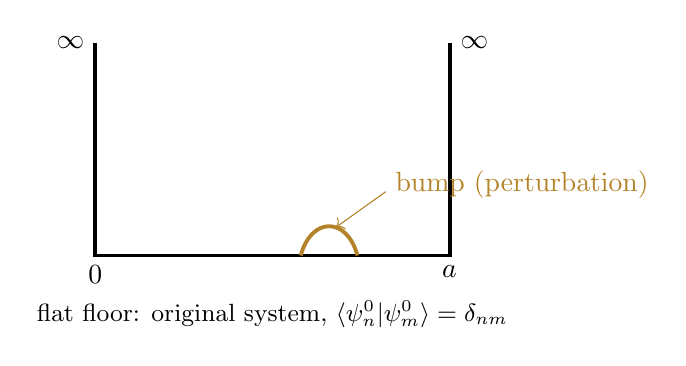
\begin{tikzpicture}[scale=0.9]
  \draw[line width=1.4pt] (0,3) -- (0,0) -- (5,0) -- (5,3);
  \draw[line width=1.4pt,exframe] (2.9,0) .. controls (3.05,0.55) and (3.55,0.55) .. (3.7,0);
  \node[below] at (0,0) {$0$};
  \node[below] at (5,0) {$a$};
  \node at (-0.35,3) {$\infty$};
  \node at (5.35,3) {$\infty$};
  \draw[->,exframe] (4.1,0.9) -- (3.4,0.4);
  \node[exframe,right] at (4.1,1.0) {bump (perturbation)};
  \node[below,align=center] at (2.5,-0.5) {\small flat floor: original system, $\langle\psi_n^0|\psi_m^0\rangle=\delta_{nm}$};
\end{tikzpicture}
\end{center}

\textbf{Known (original) problem:}
\[
\hat H^0 |\psi_n^0\rangle = E_n^0 |\psi_n^0\rangle, \qquad \langle \psi_n^0 | \psi_m^0 \rangle = \delta_{nm}
\]
\textbf{Wanted (perturbed) problem:} $\hat H|\psi_n\rangle = E_n |\psi_n\rangle$, with
\[
\hat H = \hat H^0 + \lambda \hat H' \qquad (\hat H^0 \text{ dominant},\ \lambda\hat H' \text{ a small deviation}).
\]
Expand the eigenstates and eigenvalues in powers of the bookkeeping parameter $\lambda$:
\begin{align*}
|\psi_n\rangle &= |\psi_n^0\rangle + \lambda|\psi_n^1\rangle + \lambda^2|\psi_n^2\rangle + \cdots \\
E_n &= E_n^0 + \lambda E_n^1 + \lambda^2 E_n^2 + \cdots
\end{align*}
Substituting into $\hat H|\psi_n\rangle = E_n|\psi_n\rangle$ gives
\[
(\hat H^0 + \lambda\hat H')\big[|\psi_n^0\rangle + \lambda|\psi_n^1\rangle + \lambda^2|\psi_n^2\rangle + \cdots\big] = (E_n^0 + \lambda E_n^1 + \lambda^2 E_n^2 + \cdots)\big[|\psi_n^0\rangle + \lambda|\psi_n^1\rangle + \lambda^2|\psi_n^2\rangle + \cdots\big]
\]
Collecting equal powers of $\lambda$:
\begin{align*}
\lambda^0:\quad & \hat H^0|\psi_n^0\rangle = E_n^0|\psi_n^0\rangle \\
\lambda^1:\quad & \hat H^0|\psi_n^1\rangle + \hat H'|\psi_n^0\rangle = E_n^1|\psi_n^0\rangle + E_n^0|\psi_n^1\rangle \\
\lambda^2:\quad & \hat H^0|\psi_n^2\rangle + \hat H'|\psi_n^1\rangle = E_n^0|\psi_n^2\rangle + E_n^1|\psi_n^1\rangle + E_n^2|\psi_n^0\rangle
\end{align*}

\textbf{*** Intuition:} $\lambda$ only keeps track of the order of smallness; it is set to $1$ at the end (it is absorbed in $\hat H'$ below). Each order gives one equation that is solved by projecting onto the known states $|\psi_m^0\rangle$.

\textbf{*** Study Note (normalization):} The first-order state is expanded in the complete basis, $|\psi_n^1\rangle = \sum_{m\ne n} c_m^{(n)}|\psi_m^0\rangle + c_n^{(n)}|\psi_n^0\rangle$. The $|\psi_n^0\rangle$ component drops out of the first-order equation (its coefficient is $E_n^0-E_n^0=0$), so it is fixed by the normalization choice $\langle\psi_n^0|\psi_n^1\rangle=0$, i.e.\ $c_n^{(n)}=0$. This is used below.

\subsection{First-Order Correction to the Energy}
Take the inner product of the $\lambda^1$ equation with $\langle\psi_n^0|$:
\[
\langle\psi_n^0|\hat H^0|\psi_n^1\rangle + \langle\psi_n^0|\hat H'|\psi_n^0\rangle = E_n^1\langle\psi_n^0|\psi_n^0\rangle + E_n^0\langle\psi_n^0|\psi_n^1\rangle
\]
Since $\hat H^0$ is Hermitian, $\langle\psi_n^0|\hat H^0|\psi_n^1\rangle = E_n^0\langle\psi_n^0|\psi_n^1\rangle$, which cancels the last term. Hence
\begin{thm}{First-Order Energy Correction}
\[
E_n^{1} = \langle\psi_n^0|\hat H'|\psi_n^0\rangle
\]
\end{thm}
\textbf{*** Intuition:} To first order the energy shift is just the \textit{expectation value of the perturbation in the unperturbed state}; the state itself has not yet had time to adjust.

\subsection{First-Order Correction to the Wavefunction}
Rewrite the $\lambda^1$ equation as
\[
(\hat H^0 - E_n^0)|\psi_n^1\rangle = -(\hat H' - E_n^1)|\psi_n^0\rangle \qquad (\text{everything on the right is known}).
\]
Expand $|\psi_n^1\rangle = \sum_{m\ne n} c_m^{(n)}|\psi_m^0\rangle$ (the $m=n$ term has coefficient zero). The left side becomes $\sum_{m\ne n} c_m^{(n)}(E_m^0 - E_n^0)|\psi_m^0\rangle$. Take the inner product with $\langle\psi_\ell^0|$, $\ell\neq n$:
\[
(E_\ell^0 - E_n^0)\,c_\ell^{(n)} = -\langle\psi_\ell^0|\hat H'|\psi_n^0\rangle + E_n^1\underbrace{\langle\psi_\ell^0|\psi_n^0\rangle}_{\delta_{\ell n}=0}
\]
\begin{thm}{First-Order Wavefunction Correction}
\[
c_m^{(n)} = \frac{\langle\psi_m^0|\hat H'|\psi_n^0\rangle}{E_n^0 - E_m^0}, \qquad
|\psi_n^1\rangle = \sum_{m\ne n}\frac{\langle\psi_m^0|\hat H'|\psi_n^0\rangle}{E_n^0 - E_m^0}\,|\psi_m^0\rangle
\]
\end{thm}
\textbf{*** Intuition:} The perturbation mixes in the other unperturbed states. The mixing is strong when the matrix element $\langle m|\hat H'|n\rangle$ is large and when the unperturbed levels are close ($E_n^0 - E_m^0$ small).

\textbf{*** Study Note (validity):} The expansion is trustworthy only if $\big|\langle\psi_m^0|\hat H'|\psi_n^0\rangle\big| \ll |E_n^0 - E_m^0|$. If two levels are degenerate the denominator vanishes and the formula breaks down; that case needs the degenerate theory of Section~\ref{ap:sec:deg}.

\subsection{Second-Order Correction to the Energy}
Take the inner product of the $\lambda^2$ equation with $\langle\psi_n^0|$. The $\hat H^0$ term cancels the $E_n^0\langle\psi_n^0|\psi_n^2\rangle$ term as before, leaving
\[
\langle\psi_n^0|\hat H'|\psi_n^1\rangle = E_n^1\langle\psi_n^0|\psi_n^1\rangle + E_n^2\langle\psi_n^0|\psi_n^0\rangle
\]
Now $\langle\psi_n^0|\psi_n^1\rangle = \sum_{m\ne n}c_m^{(n)}\delta_{nm} = 0$, so
\begin{align*}
E_n^2 = \langle\psi_n^0|\hat H'|\psi_n^1\rangle
&= \sum_{m\ne n} c_m^{(n)}\langle\psi_n^0|\hat H'|\psi_m^0\rangle
= \sum_{m\ne n}\langle\psi_n^0|\hat H'|\psi_m^0\rangle\,\frac{\langle\psi_m^0|\hat H'|\psi_n^0\rangle}{E_n^0 - E_m^0}
\end{align*}
\begin{thm}{Second-Order Energy Correction}
\[
E_n^{(2)} = \sum_{m\ne n}\frac{\big|\langle\psi_m^0|\hat H'|\psi_n^0\rangle\big|^2}{E_n^0 - E_m^0},
\qquad
E_n = E_n^{(0)} + E_n^{(1)} + E_n^{(2)} + \cdots
\]
Here $E_n^{(0)}$ is the unperturbed energy, $E_n^{(1)}$ the first-order and $E_n^{(2)}$ the second-order correction.
\end{thm}
\textbf{*** Memory Rule:} First order: one matrix element on the diagonal. Second order: $|\text{off-diagonal element}|^2$ divided by the energy gap, summed over all other states, with the denominator $E_n^0 - E_m^0$ (state $n$ first).

\textbf{*** Study Note:} For the \textbf{ground state} every denominator $E_0^0 - E_m^0$ is negative, so $E_0^{(2)}\le 0$: second-order perturbation always \textit{lowers} the ground-state energy (levels repel; the state is pushed away from the levels above it). Conversely, a level is pushed up by states below it and down by states above it.

\textbf{*** Exam Tip:} Before computing an infinite sum, check selection rules: most matrix elements vanish by parity or angular momentum, often leaving only two terms (see the oscillator example below).

\begin{prob}{Example: Charged Oscillator in a Weak Electric Field}
A particle of charge $q$ and mass $m$, moving in a 1D harmonic potential of frequency $\omega$, is subject to a ``weak'' electric field $E$ in the $x$-direction. Calculate the eigenvalues of the Hamiltonian (and compare with perturbation theory).

\textbf{Solution:} $\hat H = \hat H^0 + \hat H'$ with
\[
\hat H^0 = -\frac{\hbar^2}{2m}\frac{d^2}{dx^2} + \frac12 m\omega^2x^2, \qquad \hat H' = qEx
\]
\textbf{Exact route.} Change variable $y = x + \dfrac{qE}{m\omega^2}$. Completing the square,
\[
\hat H = -\frac{\hbar^2}{2m}\frac{d^2}{dy^2} + \frac12 m\omega^2y^2 - \frac{q^2E^2}{2m\omega^2}
\]
so the oscillator spectrum is simply shifted:
\[
\boxed{E_n = \Big(n+\tfrac12\Big)\hbar\omega - \frac{q^2E^2}{2m\omega^2}}
\]
\textbf{Perturbation theory.} First order: $E_n^{1} = qE\langle n|\hat x|n\rangle = 0$ (odd integrand). Second order:
\[
E_n^{2} = q^2E^2\sum_{m\ne n}\frac{|\langle m|\hat x|n\rangle|^2}{E_n^0 - E_m^0} = -\frac{q^2E^2}{2m\omega^2}
\]
Only $m = n-1$ and $m = n+1$ contribute.
\end{prob}

\begin{prob}{Example: Charged Oscillator in a Weak Electric Field (continued)}
\textbf{*** Complete Solution of the second-order sum:} Use $\hat x = \sqrt{\hbar/2m\omega}\,(\hat a + \hat a^\dagger)$, so
\[
\langle n-1|\hat x|n\rangle = \sqrt{\frac{\hbar}{2m\omega}}\sqrt n, \qquad \langle n+1|\hat x|n\rangle = \sqrt{\frac{\hbar}{2m\omega}}\sqrt{n+1}
\]
with $E_n^0 - E_{n-1}^0 = +\hbar\omega$ and $E_n^0 - E_{n+1}^0 = -\hbar\omega$:
\begin{align*}
E_n^{2} &= q^2E^2\,\frac{\hbar}{2m\omega}\left[\frac{n}{\hbar\omega} + \frac{n+1}{-\hbar\omega}\right]
= q^2E^2\,\frac{\hbar}{2m\omega}\cdot\frac{-1}{\hbar\omega} = -\frac{q^2E^2}{2m\omega^2}
\end{align*}
which agrees with the exact result.

\textbf{*** Study Note:} The shift is the same for every level and the series stops at second order here, so perturbation theory reproduces the exact answer; this is a useful test case for any new formula. Physically the oscillator is polarized by the field and its equilibrium moves to $x_0 = -qE/m\omega^2$.
\end{prob}

%==============================================================================
\section{Time-Independent Perturbation Theory: Degenerate Case}\label{ap:sec:deg}
%==============================================================================

\subsection{Two-Fold Degeneracy}
If the unperturbed states are degenerate, the non-degenerate formulas fail because of the vanishing denominators $E_n^0-E_m^0$. Take a 2-fold degenerate level:
\[
\hat H^0|\psi_a^0\rangle = E^0|\psi_a^0\rangle, \qquad \hat H^0|\psi_b^0\rangle = E^0|\psi_b^0\rangle, \qquad \langle\psi_a^0|\psi_b^0\rangle = 0
\]
Any combination is also an eigenstate of $\hat H^0$ with the same energy:
\[
|\psi^0\rangle = \alpha|\psi_a^0\rangle + \beta|\psi_b^0\rangle, \qquad \hat H^0|\psi^0\rangle = E^0|\psi^0\rangle
\]
The perturbation breaks the degeneracy: as it is switched on, the single level splits into two (figure below). The zeroth-order state that the perturbed state tends to is a \textit{particular} combination ($\alpha,\beta$ fixed by $\hat H'$), which the theory must determine.

\begin{center}
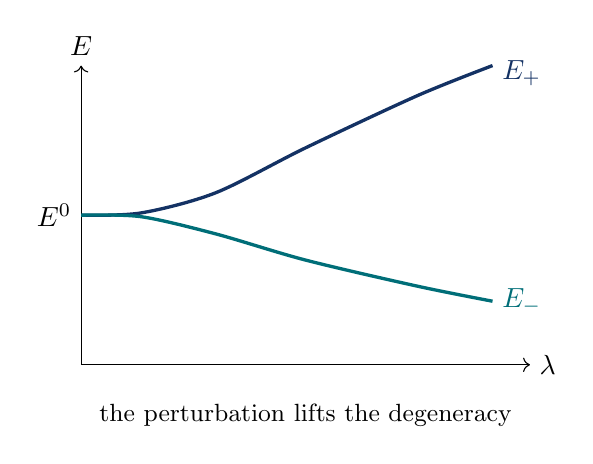
\begin{tikzpicture}[scale=0.95]
  \draw[->] (0,0) -- (6,0) node[right] {$\lambda$};
  \draw[->] (0,0) -- (0,4) node[above] {$E$};
  \draw[very thick,primary] plot[smooth] coordinates {(0,2) (0.8,2.03) (1.8,2.3) (3,2.9) (4.5,3.6) (5.5,4.0)};
  \draw[very thick,secondary] plot[smooth] coordinates {(0,2) (0.8,1.98) (1.8,1.75) (3,1.4) (4.5,1.05) (5.5,0.85)};
  \node[primary,right] at (5.5,3.9) {$E_+$};
  \node[secondary,right] at (5.5,0.85) {$E_-$};
  \node[left] at (0,2) {$E^0$};
  \node[below,align=center] at (3,-0.4) {\small the perturbation lifts the degeneracy};
\end{tikzpicture}
\end{center}

The $\lambda^1$ equation is
\[
\hat H'|\psi^0\rangle + \hat H^0|\psi^1\rangle = E^0|\psi^1\rangle + E^1|\psi^0\rangle
\]
Take the inner product with $\langle\psi_a^0|$. By Hermiticity $\langle\psi_a^0|\hat H^0|\psi^1\rangle = E^0\langle\psi_a^0|\psi^1\rangle$, which cancels, leaving
\[
\langle\psi_a^0|\hat H'|\psi^0\rangle = E^1\langle\psi_a^0|\psi^0\rangle
\;\Longrightarrow\;
\alpha\langle\psi_a^0|\hat H'|\psi_a^0\rangle + \beta\langle\psi_a^0|\hat H'|\psi_b^0\rangle = E^1\alpha \tag{I}
\]
Taking the inner product with $\langle\psi_b^0|$ instead:
\[
\alpha\langle\psi_b^0|\hat H'|\psi_a^0\rangle + \beta\langle\psi_b^0|\hat H'|\psi_b^0\rangle = E^1\beta \tag{II}
\]
Define the matrix elements of the perturbation inside the degenerate subspace:
\[
W_{aa} = \langle\psi_a^0|\hat H'|\psi_a^0\rangle,\quad W_{bb} = \langle\psi_b^0|\hat H'|\psi_b^0\rangle,\quad W_{ab} = \langle\psi_a^0|\hat H'|\psi_b^0\rangle,\quad W_{ba} = \langle\psi_b^0|\hat H'|\psi_a^0\rangle
\]
Then (I) and (II) read
\[
\alpha(W_{aa} - E^1) + \beta W_{ab} = 0, \qquad \alpha W_{ba} + \beta(W_{bb} - E^1) = 0
\]
A nontrivial solution $(\alpha,\beta)$ exists only if the determinant vanishes:
\begin{thm}{Secular Equation (Two-Fold Degeneracy)}
\[
\det\begin{pmatrix} W_{aa}-E^1 & W_{ab} \\ W_{ba} & W_{bb}-E^1 \end{pmatrix} = 0
\]
Using $W_{ab} = W_{ba}^*$ this is $(E^1)^2 - (W_{aa}+W_{bb})E^1 + W_{aa}W_{bb} - |W_{ab}|^2 = 0$, with roots
\[
E^1_{\pm} = \frac12\left[(W_{aa}+W_{bb}) \pm \sqrt{(W_{aa}-W_{bb})^2 + 4|W_{ab}|^2}\right]
\]
\end{thm}
\textbf{*** Study Note:} The discriminant is non-negative, so both roots are real, and they are distinct unless $W_{aa}=W_{bb}$ and $W_{ab}=0$ (then the degeneracy survives at first order). If $W_{ab}=0$ the roots are simply $W_{aa}$ and $W_{bb}$, and $|\psi_a^0\rangle,|\psi_b^0\rangle$ are already the ``good'' states. In general the ratio is fixed by $\beta/\alpha = (E^1_\pm - W_{aa})/W_{ab}$.

\textbf{*** Intuition:} Degenerate perturbation theory says: \textit{inside the degenerate subspace, diagonalize the perturbation}. The eigenvalues are the first-order energy shifts, the eigenvectors are the correct zeroth-order states.

\subsection{\texorpdfstring{$n$}{n}-Fold Degeneracy}
For an $n$-fold degenerate level write $|\psi^0\rangle = c_1|\psi_1^0\rangle + \cdots + c_n|\psi_n^0\rangle$. The same steps give the eigenvalue problem for the $W$-matrix, $W_{ij} = \langle\psi_i^0|\hat H'|\psi_j^0\rangle$:
\begin{thm}{$W$-Matrix Equation}
\[
\begin{pmatrix} W_{11} & W_{12} & \cdots & W_{1n}\\ W_{21} & W_{22} & \cdots & W_{2n}\\ \vdots & & \ddots & \vdots\\ W_{n1} & W_{n2} & \cdots & W_{nn}\end{pmatrix}
\begin{pmatrix} c_1\\ \vdots\\ c_n\end{pmatrix} = E^1\begin{pmatrix} c_1\\ \vdots\\ c_n\end{pmatrix}
\]
The $n$ roots of $\det(W - E^1\mathbb{1}) = 0$ are the first-order shifts; each eigenvector gives the corresponding good zeroth-order state.
\end{thm}
\textbf{*** Exam Tip:} Procedure: (1) list the degenerate states, (2) compute \textit{all} $W_{ij}$, (3) write the $W$-matrix, (4) solve $\det(W-E^1)=0$, (5) quote $E = E^0 + E^1$. Use $\operatorname{tr}W=\sum E^1_i$ as a check.

\subsection{Example: Infinite Cubic Well}
\begin{prob}{Example: 3D Infinite Cubic Well with a Perturbation}
\begin{gather*}
V(x,y,z) = \begin{cases} 0, & 0<x<a,\ 0<y<a,\ 0<z<a\\ \infty, & \text{otherwise}\end{cases}\\
\psi^0_{n_xn_yn_z} = \Big(\frac2a\Big)^{3/2}\sin\frac{n_x\pi x}{a}\sin\frac{n_y\pi y}{a}\sin\frac{n_z\pi z}{a}
\end{gather*}
\[
E^0_{n_xn_yn_z} = \frac{\pi^2\hbar^2}{2ma^2}\,(n_x^2+n_y^2+n_z^2), \qquad n_x,n_y,n_z = 1,2,\ldots
\]
The perturbation is
\[
\hat H' = \begin{cases} V_0, & 0<x<\tfrac a2,\ 0<y<\tfrac a2\ (\text{any } z)\\ 0, & \text{otherwise}\end{cases}
\]
\begin{center}
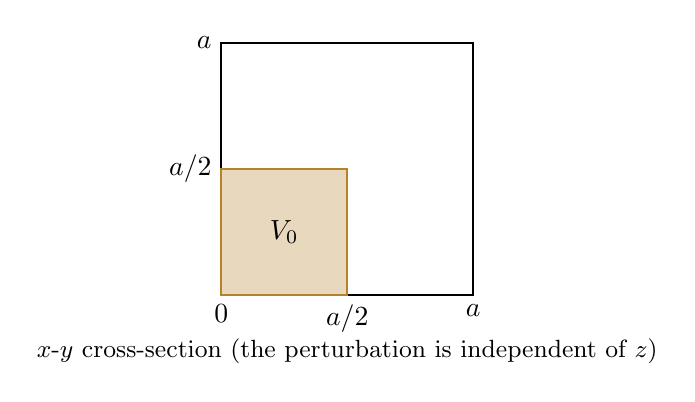
\begin{tikzpicture}[scale=0.8]
  \draw[thick] (0,0) rectangle (4,4);
  \fill[exframe!30] (0,0) rectangle (2,2);
  \draw[exframe,thick] (0,0) rectangle (2,2);
  \node at (1,1) {$V_0$};
  \node[below] at (0,0) {$0$}; \node[below] at (2,0) {$a/2$}; \node[below] at (4,0) {$a$};
  \node[left] at (0,2) {$a/2$}; \node[left] at (0,4) {$a$};
  \node[below] at (2,-0.55) {\small $x$-$y$ cross-section (the perturbation is independent of $z$)};
\end{tikzpicture}
\end{center}
\end{prob}

\begin{prob}{Example: 3D Infinite Cubic Well (continued): Ground State and First Excited Level}
\textbf{Ground state} $E_0^0 = E^0_{111} = \dfrac{3\pi^2\hbar^2}{2ma^2}$ is non-degenerate:
\[
E_0^{(1)} = \langle\psi^0_{111}|\hat H'|\psi^0_{111}\rangle = \Big(\frac2a\Big)^3V_0\int_0^{a/2}\!\sin^2\frac{\pi x}{a}dx\int_0^{a/2}\!\sin^2\frac{\pi y}{a}dy\int_0^a\!\sin^2\frac{\pi z}{a}dz = \frac14 V_0
\]
This is the correction to the ground-state energy.

\textbf{First excited level:} $(n_x,n_y,n_z) = (1,2,1),(2,1,1),(1,1,2)$, 3-fold degenerate with $E_1^0 = E^0_{121} = \dfrac{3\pi^2\hbar^2}{ma^2}$. Write
\[
|\psi^0\rangle = c_1|\psi^0_{112}\rangle + c_2|\psi^0_{121}\rangle + c_3|\psi^0_{211}\rangle
\]
and build $W_{ij}=\langle\psi^0_i|\hat H'|\psi^0_j\rangle=\int d^3r\,\psi_i^{0*}\hat H'\psi_j^0$. The result is $W_{11}=W_{22}=W_{33}=\tfrac14V_0$ and a single non-zero off-diagonal pair $W_{23}=W_{32}=\dfrac{16}{9\pi^2}V_0$, so
\[
\det\begin{pmatrix}\tfrac14V_0 - E^1 & 0 & 0\\ 0 & \tfrac14V_0 - E^1 & \tfrac{16}{9\pi^2}V_0\\ 0 & \tfrac{16}{9\pi^2}V_0 & \tfrac14V_0 - E^1\end{pmatrix} = 0
\]
\end{prob}

\begin{prob}{Example: 3D Infinite Cubic Well (completed solution)}
\textbf{*** Study Note (ordering of the states):} The notebook lists the states in the order $121,\,211,\,112$ and then states $W_{12}=W_{13}=0$, $W_{23}=\frac{16}{9\pi^2}V_0$. That statement matches the matrix above only if the \textit{decoupled} state ($112$) is labelled first. With the order $121,211,112$ the correct elements are $W_{12}\neq 0$ and $W_{13}=W_{23}=0$. The matrix, eigenvalues and conclusions are unchanged; the ordering $112,121,211$ is used here.

\textbf{*** Complete Solution:} Diagonal elements, for example $|112\rangle$:
\[
W_{11} = \frac{8}{a^3}V_0\underbrace{\int_0^{a/2}\!\sin^2\tfrac{\pi x}{a}dx}_{a/4}\underbrace{\int_0^{a/2}\!\sin^2\tfrac{\pi y}{a}dy}_{a/4}\underbrace{\int_0^{a}\!\sin^2\tfrac{2\pi z}{a}dz}_{a/2} = \frac{V_0}{4}
\]
and in the same way $W_{22}=W_{33}=V_0/4$ (over $[0,a/2]$ both $\sin^2(\pi u/a)$ and $\sin^2(2\pi u/a)$ integrate to $a/4$).

Off-diagonal elements. $W_{12}=\langle 112|\hat H'|121\rangle$ contains $\int_0^a\sin\frac{2\pi z}{a}\sin\frac{\pi z}{a}\,dz=0$ (orthogonality), so $W_{12}=W_{13}=0$. For $W_{23}=\langle121|\hat H'|211\rangle$ the $z$-integral is $\int_0^a\sin^2\frac{\pi z}{a}dz = \frac a2$, and with $\sin A\sin 2A = 2\sin^2A\cos A$:
\[
\int_0^{a/2}\sin\frac{\pi x}{a}\sin\frac{2\pi x}{a}\,dx = \frac a\pi\Big[\tfrac23\sin^3u\Big]_0^{\pi/2} = \frac{2a}{3\pi}
\]
The $y$-integral is the same. Therefore
\[
W_{23} = \frac{8}{a^3}V_0\Big(\frac{2a}{3\pi}\Big)^2\frac a2 = \frac{16}{9\pi^2}V_0
\]
Eigenvalues: $\big(\tfrac14V_0-E^1\big)\Big[\big(\tfrac14V_0-E^1\big)^2 - \big(\tfrac{16}{9\pi^2}V_0\big)^2\Big]=0$, hence
\[
E^1 = \tfrac14V_0, \qquad E^1 = \Big(\tfrac14 \pm \tfrac{16}{9\pi^2}\Big)V_0 \approx 0.430\,V_0,\ 0.070\,V_0
\]
Good zeroth-order states: $|112\rangle$ for $E^1=\frac14V_0$, and $\frac1{\sqrt2}\big(|121\rangle \pm |211\rangle\big)$ for $E^1 = \frac14V_0 \pm \frac{16}{9\pi^2}V_0$. The three-fold degeneracy is completely lifted:
\[
E = \frac{3\pi^2\hbar^2}{ma^2} + E^1
\]
\textbf{*** Verification:} $\operatorname{tr}W = \frac34V_0 = \frac14V_0 + \big(\frac14+\frac{16}{9\pi^2}\big)V_0 + \big(\frac14-\frac{16}{9\pi^2}\big)V_0$. \checkmark

\textbf{*** Intuition:} $\hat H'$ is symmetric under $x\leftrightarrow y$, so the symmetric and antisymmetric combinations of $|121\rangle,|211\rangle$ are the natural good states, while $|112\rangle$ (which is itself symmetric and has a different $z$-dependence) decouples.
\end{prob}

\subsection{Good States and Commuting Operators}
\begin{thm}{Theorem: Good States from a Commuting Operator}
Let $\hat A$ be a Hermitian operator that commutes with $\hat H^0$ and with $\hat H'$. If $|\psi_a^0\rangle$ and $|\psi_b^0\rangle$ (the degenerate eigenfunctions of $\hat H^0$) are also eigenfunctions of $\hat A$ with \textbf{distinct eigenvalues}, then
\[
\langle\psi_a^0|\hat H'|\psi_b^0\rangle = 0
\]
\textbf{Proof:} Let $\hat A|\psi_a^0\rangle = \mu|\psi_a^0\rangle$, $\hat A|\psi_b^0\rangle = \nu|\psi_b^0\rangle$, $\mu\ne\nu$, and $[\hat A,\hat H']=0$. Then
\[
0 = \langle\psi_a^0|(\hat A\hat H' - \hat H'\hat A)|\psi_b^0\rangle = (\mu-\nu)\langle\psi_a^0|\hat H'|\psi_b^0\rangle
\]
and since $\mu\ne\nu$, $\langle\psi_a^0|\hat H'|\psi_b^0\rangle = 0$. \qed
\end{thm}
In that case the energies are simply $E^1_+ = \langle\psi_a^0|\hat H'|\psi_a^0\rangle$ and $E^1_- = \langle\psi_b^0|\hat H'|\psi_b^0\rangle$ (no matrix diagonalization needed).

\textbf{*** Memory Rule:} Look for an operator that commutes with \textit{both} $\hat H^0$ and $\hat H'$ (a symmetry of the full problem) and label the degenerate states by its eigenvalues. For hydrogen with spin-orbit coupling these are $\hat J^2,\hat J_z$, not $\hat L_z,\hat S_z$ (see Section~\ref{ap:sec:hyd}).

\textbf{*** Common mistakes:} (a) using the non-degenerate formula $E^{(2)}$ when two levels coincide, (b) forgetting that off-diagonal $W_{ij}$ matter even when the diagonal ones are equal, (c) taking the basis states themselves as good states without checking $W_{ab}=0$, (d) dropping the factor $E_n^0-E_m^0$ order (it is $n$ first).

%==============================================================================
\section{Applications to Hydrogen: Fine Structure and the Zeeman Effect}\label{ap:sec:hyd}
%==============================================================================

\subsection{Spin-Orbit Coupling}
In the rest frame of the electron the proton circles around it and produces a magnetic field. For an electron moving with velocity $\vec v$ in the proton's electric field $\vec E$ (Gaussian units):
\[
\vec B = -\frac1c\,\vec v\times\vec E = -\frac{1}{m_ec}\,\vec p\times\vec E = \frac{1}{m_ec}\,(\vec E\times\vec p)
\]
\begin{center}
\begin{tikzpicture}[scale=0.9]
  \draw[dashed] (0,0) circle (1.6);
  \node at (0,0) {$+$};
  \fill (1.13,1.13) circle (0.09);
  \node[right] at (1.25,1.2) {$e^-$};
  \draw[->,thick,exframe] (1.13,1.13) -- (0.6,1.7) node[above left] {$\vec v$};
  \node[below,align=center] at (0,-1.9) {\small hydrogen atom: the electron sees the proton's field as a magnetic field $\vec B$};
\end{tikzpicture}
\end{center}
For a central potential, with $V(r) = -e\phi(r)$ and $\vec E = -\nabla\phi$:
\[
\vec E(\vec r) = \frac{1}{e}\frac{\vec r}{r}\frac{dV}{dr}
\quad\Longrightarrow\quad
\vec B = \frac{1}{e\,m_e c}\,\frac1r\frac{dV}{dr}\,(\vec r\times\vec p) = \frac{1}{m_e e c\, r}\frac{dV}{dr}\,\vec L
\]
The electron's spin magnetic moment is $\vec\mu_s = -\dfrac{e}{m_ec}\vec S$, and the interaction energy $-\vec\mu_s\cdot\vec B$ gives the spin-orbit Hamiltonian
\begin{thm}{Spin-Orbit Hamiltonian}
\[
\hat H_{\text{soc}} = \lambda\,\hat{\vec L}\cdot\hat{\vec S}, \qquad \lambda = \lambda(r) = \frac{1}{2m_e^2c^2}\frac1r\frac{dV}{dr}\ \xrightarrow{\,V=-e^2/r\,}\ \frac{e^2}{2m_e^2c^2}\frac{1}{r^3}
\]
\end{thm}
\textbf{*** Study Note:} The naive calculation above gives a prefactor $1/(m_e^2c^2)$; the factor $\tfrac12$ in $\lambda$ is the \textbf{Thomas precession} correction (the electron's rest frame is accelerating). The notebook uses the correct final form $\lambda = e^2/(2m_e^2c^2r^3)$. In SI units replace $e^2\to e^2/4\pi\varepsilon_0$.

The hydrogen problem with spin-orbit coupling is
\[
\hat H = \underbrace{\frac{\hat p^2}{2m_e} - \frac{e^2}{r}}_{\hat H^0} + \underbrace{\frac{e^2}{2m_e^2c^2r^3}\,\hat{\vec L}\cdot\hat{\vec S}}_{\hat H_{\text{soc}}} = \hat H^0 + \hat H'
\]

\subsection{Choice of Basis: Which States Are Good?}
\begin{itemize}
    \item \textbf{Uncoupled basis} $|n,l,s,m_l,m_s\rangle$, eigenstates of $\{\hat L^2,\hat S^2,\hat L_z,\hat S_z\}$. This is \textbf{not good}: $\hat{\vec L}\cdot\hat{\vec S}$ does not commute with $\hat L_z$ or $\hat S_z$, so $\hat H_{\text{soc}}$ is not diagonal in it and the degenerate levels are mixed.
    \item \textbf{Coupled basis} $|n,j,m_j,l,s\rangle$, eigenstates of $\{\hat J^2,\hat J_z,\hat L^2,\hat S^2\}$ with $\hat{\vec J} = \hat{\vec L}+\hat{\vec S}$. This is \textbf{good}: $\hat J^2$ and $\hat J_z$ commute with $\hat H^0$ and with $\hat H_{\text{soc}}$, so by the theorem of Section~\ref{ap:sec:deg} the off-diagonal elements between different $j,m_j$ vanish.
\end{itemize}
Using $\hat{\vec L}\cdot\hat{\vec S} = \tfrac12\big(\hat J^2 - \hat L^2 - \hat S^2\big)$, the first-order energy is
\[
E_{\text{soc}} = \langle n,j,m_j,l,s|\,\lambda\hat{\vec L}\cdot\hat{\vec S}\,|n,j,m_j,l,s\rangle
= \frac{e^2\hbar^2}{4m_e^2c^2}\Big[j(j+1) - l(l+1) - s(s+1)\Big]\Big\langle n l\Big|\frac1{r^3}\Big|n l\Big\rangle
\]
with $s(s+1)=\tfrac34$ and the standard hydrogen expectation value
\[
\Big\langle n l\Big|\frac{1}{r^3}\Big|n l\Big\rangle = \frac{2}{n^3\,l(l+1)(2l+1)\,a_0^3}
\]
\begin{thm}{Spin-Orbit Energy of Hydrogen}
\begin{align*}
E_{nlj} &= -\frac{e^2}{2a_0}\frac1{n^2} + E_{\text{soc}}\\
E^{\text{soc}}_n &= \frac{e^2\hbar^2}{2m_e^2c^2}\left[\frac{j(j+1)-l(l+1)-\tfrac34}{n^3\,l(l+1)(2l+1)\,a_0^3}\right]\\
&= \frac{|E_n^{(0)}|}{n}\,\alpha^2\left[\frac{j(j+1)-l(l+1)-\tfrac34}{l(l+1)(2l+1)}\right]
\end{align*}
with $E_n^{(0)} = -\dfrac{e^2}{2a_0n^2} = -\dfrac{\alpha^2m_ec^2}{2n^2}$, fine-structure constant $\alpha = \dfrac{\hbar}{m_eca_0} = \dfrac{e^2}{\hbar c}\simeq\dfrac1{137}$, and Bohr radius $a_0 = \dfrac{\hbar^2}{m_ee^2}$.
\end{thm}
\textbf{*** Study Note (sign):} In the notebook the last form is written with $E_n^{(0)}$ (a negative number) in front. With $E_n^{(0)}<0$ that would make $E_n^{\text{soc}}$ negative for $j=l+\tfrac12$, which contradicts the first form (positive for $j=l+\frac12$). The correct prefactor is $|E_n^{(0)}| = -E_n^{(0)}$, as written above. Check: $|E_n^{(0)}|\alpha^2/n = \alpha^4m_ec^2/(2n^3)$, and $\frac{e^2\hbar^2}{2m_e^2c^2a_0^3} = |E_1^{(0)}|\alpha^2$. \checkmark

\textbf{*** Study Note:} For $l=0$ the expression is $0/0$ but there is no spin-orbit energy ($\hat{\vec L}=0$, so $\hat H_{\text{soc}}=0$). The relative size is $\sim\alpha^2\approx 5\times10^{-5}$ of $E_n^{(0)}$, which is why it is called \textit{fine} structure.

\subsection{Relativistic Correction}
The kinetic energy is $\hat T = \sqrt{\hat p^2c^2 + m_e^2c^4} - m_ec^2 = m_ec^2\sqrt{1+\dfrac{\hat p^2}{m_e^2c^2}} - m_ec^2$. Expanding in $p/m_ec$:
\[
\hat T = \frac{\hat p^2}{2m_e} - \frac18\frac{\hat p^4}{m_e^3c^2} + \cdots
\]
so the Hamiltonian with relativistic correction is
\[
\hat H = \underbrace{\frac{\hat p^2}{2m_e} - \frac{e^2}{r}}_{\hat H^0} \underbrace{-\,\frac{\hat p^4}{8m_e^3c^2}}_{\hat H_R} = \hat H^0 + \hat H_R
\]
First-order perturbation correction:
\[
E'_{\text{Rel}} = \Big\langle n\,l\,s\,j\,m_j\Big|\hat p^4\Big|n\,l\,s\,j\,m_j\Big\rangle\Big(-\frac{1}{8m_e^3c^2}\Big) = -\frac{\alpha^4m_ec^2}{8n^4}\Big(\frac{8n}{2l+1}-3\Big)
\]
\textbf{*** Study Note (sign):} The notebook shows the same quantity once more as $\frac{\alpha^2|E_n^{(0)}|}{4n^2}\big(\frac{8n}{2l+1}-3\big)$ without the minus sign. Since $\frac{\alpha^2|E_n^{(0)}|}{4n^2}=\frac{\alpha^4m_ec^2}{8n^4}$, the correct form is $E'_{\text{Rel}} = -\dfrac{\alpha^2|E_n^{(0)}|}{4n^2}\Big(\dfrac{8n}{2l+1}-3\Big)$, always negative (relativistic effects lower the energy).

\textbf{*** Complete Solution (evaluating $\langle\hat p^4\rangle$):} From $\hat H^0|\psi\rangle = E_n|\psi\rangle$ we have $\hat p^2 = 2m_e(E_n + e^2/r)$ on the state, so
\[
\langle\hat p^4\rangle = 4m_e^2\Big\langle\Big(E_n+\frac{e^2}{r}\Big)^2\Big\rangle = 4m_e^2\Big[E_n^2 + 2E_ne^2\Big\langle\frac1r\Big\rangle + e^4\Big\langle\frac1{r^2}\Big\rangle\Big]
\]
with $\langle 1/r\rangle = \dfrac{1}{n^2a_0}$ and $\langle 1/r^2\rangle = \dfrac{1}{(l+\frac12)\,n^3a_0^2}$, $E_n=-\dfrac{e^2}{2a_0n^2}$:
\[
E'_{\text{Rel}} = -\frac{1}{2m_ec^2}\,\frac{e^4}{a_0^2}\Big[\frac1{4n^4} - \frac1{n^4} + \frac{2}{n^3(2l+1)}\Big]
= -\frac{e^4}{8m_ec^2a_0^2n^4}\Big(\frac{8n}{2l+1}-3\Big)
\]
and $e^4/a_0^2 = \alpha^4m_e^2c^4$ gives the result above. \checkmark

\textbf{*** Study Note:} $\hat p^4$ is a scalar and commutes with $\hat L^2,\hat L_z$, so the hydrogen states $|n,l,m\rangle$ are already good states and no degenerate diagonalization is required.

\subsection{Fine Structure}
Spin-orbit coupling plus the relativistic correction together form the \textbf{fine structure}:
\begin{thm}{Fine-Structure Correction to the Energy}
\[
E^{(1)}_{\text{FS}} = \frac{\alpha^4m_ec^2}{2n^3}\left[\frac{j(j+1)-l(l+1)-\tfrac34}{l(l+1)(2l+1)}\right] - \frac{\alpha^4m_ec^2}{8n^4}\left[\frac{8n}{2l+1}-3\right]
\]
\end{thm}
\textbf{*** Complete Solution (simplification):} For $j=l+\tfrac12$ the bracket $j(j+1)-l(l+1)-\frac34$ equals $l$; for $j=l-\tfrac12$ it equals $-(l+1)$. In both cases the two terms combine to
\[
E^{(1)}_{\text{FS}} = -\frac{\alpha^4m_ec^2}{8n^4}\Big(\frac{4n}{j+\frac12}-3\Big) = -\frac{(E_n^{(0)})^2}{2m_ec^2}\Big(\frac{4n}{j+\frac12}-3\Big)
\]
Check for $j=l+\tfrac12$: spin-orbit term $\frac{\alpha^4m_ec^2}{2n^3(l+1)(2l+1)}$; combining with the relativistic term gives $\frac{8n}{2l+1}-3-\frac{4n}{(l+1)(2l+1)} = \frac{4n}{l+1}-3 = \frac{4n}{j+1/2}-3$. \checkmark

\textbf{*** Exam Tip:} The fine-structure shift depends only on $n$ and $j$, not on $l$ separately (e.g.\ the $2S_{1/2}$ and $2P_{1/2}$ levels stay degenerate at this order).

\subsection{Anomalous Zeeman Effect}
In a magnetic field the Hamiltonian acquires
\[
\hat H_B = -\vec\mu_L\cdot\vec B - \vec\mu_s\cdot\vec B = \frac{e}{2m_ec}\,\vec L\cdot\vec B + \frac{e}{m_ec}\,\vec S\cdot\vec B
\]
Take $\vec B = B_0\hat e_z$. Then
\[
\hat H_B = \frac{eB_0}{2m_ec}\big(\hat L_z + 2\hat S_z\big) = \frac{eB_0}{2m_ec}\big(\hat J_z + \hat S_z\big) = \frac{\mu_BB_0}{\hbar}\big(\hat J_z+\hat S_z\big), \qquad \mu_B = \frac{e\hbar}{2m_ec}\ (\text{Bohr magneton})
\]
and the full Hamiltonian is
\[
\boxed{\hat H = \hat H^0 + \hat H_{\text{soc}} + \hat H_R + \hat H_B}
\]
Two limiting regimes are treated (the relativistic term is neglected in the first):
\begin{enumerate}
    \item \textbf{Strong field, $\hat H_B \gg \hat H_{\text{soc}}$:} $\hat H = \hat H^0+\hat H_B$, use the uncoupled basis $|n,l,s,m_l,m_s\rangle$:
    \[
    E^{(1)}_B = \frac{eB_0}{2m_ec}\langle n l s m_l m_s|(\hat L_z+2\hat S_z)|n l s m_l m_s\rangle = \frac{eB_0\hbar}{2m_ec}\,(m_l+2m_s)
    \]
    \begin{thm}{Paschen-Back Effect}
    \[
    E^{\prime}_{(B)} = \frac{eB_0\hbar}{2m_ec}\,(m_l + 2m_s)
    \]
    \end{thm}
    \item \textbf{Weak field, $\hat H_{FS}=\hat H_{\text{soc}}+\hat H_R \gg \hat H_B$:} $\hat H = \hat H^0+\hat H_{FS}+\hat H_B$, use the coupled basis $|n,j,m_j,l,s\rangle$:
    \[
    E^{(1)}_B = \frac{eB_0}{2m_ec}\Big[\hbar m_j + \langle n l s j m_j|\hat S_z|n l s j m_j\rangle\Big]
    \]
    By the projection theorem
    \[
    \langle\hat S_z\rangle = \frac{\langle\hat{\vec J}\cdot\hat{\vec S}\rangle}{\hbar^2j(j+1)}\,\langle\hat J_z\rangle, \qquad \hat{\vec J}\cdot\hat{\vec S} = \tfrac12\big(\hat J^2+\hat S^2-\hat L^2\big)
    \]
    which gives the Land\'e result:
    \begin{thm}{Weak-Field Zeeman Energy and the Land\'e $g$-Factor}
    \[
    E^{(1)}_B = \frac{eB_0\hbar}{2m_ec}\,g_J\,m_j, \qquad g_J = 1 + \frac{j(j+1) - l(l+1) + s(s+1)}{2j(j+1)}
    \]
    \end{thm}
\end{enumerate}
\textbf{*** Study Note (sign in the Land\'e factor):} The notebook prints the numerator as $j(j+1)-l(l+1)-s(s+1)$. Since $\langle\hat{\vec J}\cdot\hat{\vec S}\rangle = \frac{\hbar^2}{2}[j(j+1)+s(s+1)-l(l+1)]$, the $s(s+1)$ term carries a \textbf{plus} sign. Check: for $l=0$, $j=s=\tfrac12$ the free electron must give $g=2$: $1+\frac{3/4+3/4}{3/2}=2$ \checkmark (the printed sign would give $g=1$).

\textbf{*** Study Note (regimes):} The notebook labels the second regime as ``$H_{soc}\sim H_B$''; the computation with $|n,j,m_j,l,s\rangle$ as good states is valid when $\hat H_B$ is small compared with the fine structure (weak field). If $\hat H_B$ is comparable to $\hat H_{FS}$, $\hat H_B+\hat H_{FS}$ must be diagonalized inside each $m_j$ subspace.

\textbf{*** Exam Tip:} Quick values for hydrogen with $n=2$: $2S_{1/2}$: $g_J=2$; $2P_{1/2}$: $g_J=\frac23$; $2P_{3/2}$: $g_J=\frac43$. Weak-field levels split into $2j+1$ equally spaced lines (spacing $g_J\mu_BB_0$).

\textbf{*** Common mistakes:} (a) using the uncoupled basis when spin-orbit coupling is present, (b) writing $m_l+m_s$ instead of $m_l+2m_s$ (the spin $g$-factor is 2), (c) forgetting that $g_J$ depends on $l$, $s$ and $j$, (d) using $E_n^{(0)}$ instead of $|E_n^{(0)}|$ in the spin-orbit prefactor.

%==============================================================================
\section{The Variational Method}
%==============================================================================

\subsection{The Variational Principle}
\textbf{Goal:} calculate the ground-state energy $E_{GS}$ of a system whose Hamiltonian we cannot solve in the time-independent Schr\"odinger equation. The variational method provides an \textbf{upper bound} to the ground-state energy: guess a wavefunction $|\psi\rangle$ (the \textit{trial wavefunction}) and compute $\langle\hat H\rangle$.

\begin{thm}{Variational Principle}
For any normalized trial state $|\psi\rangle$,
\[
E_{GS} \le \langle\psi|\hat H|\psi\rangle = \langle\hat H\rangle
\]
(for an unnormalized state use $\langle\hat H\rangle = \langle\psi|\hat H|\psi\rangle/\langle\psi|\psi\rangle$).
\end{thm}
\textbf{Proof:} Let $\hat H|\phi_n\rangle = E_n|\phi_n\rangle$ (the eigenstates are unknown but exist and form a complete set) with $E_0\equiv E_{GS}\le E_1\le\cdots$. Expand $|\psi\rangle = \sum_nc_n|\phi_n\rangle$. Normalization gives
\[
\langle\psi|\psi\rangle = \sum_m\sum_nc_m^*c_n\underbrace{\langle\phi_m|\phi_n\rangle}_{\delta_{mn}} = \sum_n|c_n|^2 = 1
\]
and therefore
\begin{align*}
\langle\hat H\rangle &= \sum_m\sum_nc_m^*c_nE_n\delta_{mn} = \sum_nE_n|c_n|^2 = E_0|c_0|^2 + E_1|c_1|^2 + \cdots\\
&\ge E_0\sum_n|c_n|^2 = E_0 \qquad\blacksquare
\end{align*}

\textbf{*** Intuition:} $\langle\hat H\rangle$ is a weighted average of the true energies $E_n$ with weights $|c_n|^2$ summing to one, so it can never fall below the smallest one.

\textbf{*** Exam Tip (recipe):}
\begin{enumerate}[noitemsep]
    \item Choose a trial function with a free parameter (or two) and with the right qualitative shape (no nodes for the ground state, correct behaviour at infinity and at boundaries, correct symmetry).
    \item Normalize it (fixes the constant).
    \item Compute $\langle\hat H\rangle = \langle T\rangle + \langle V\rangle$ as a function of the parameter.
    \item Minimize: $\dfrac{d\langle\hat H\rangle}{d(\text{parameter})}=0$, and substitute back.
\end{enumerate}
\textbf{*** Study Note:} If the trial function contains the exact ground state for some value of the parameter, the minimum equals $E_{GS}$ exactly (the oscillator below). Because $\langle\hat H\rangle - E_0 = \sum_{n\ge1}(E_n-E_0)|c_n|^2$ and $|c_n|\sim$ the error of the wavefunction, the \textit{energy} error is second order in the \textit{wavefunction} error, which is why even a crude trial function gives a good energy.

\subsection{Example: Harmonic Oscillator}
\begin{prob}{Example: Variational Treatment of the Harmonic Oscillator}
$\hat H = -\dfrac{\hbar^2}{2m}\dfrac{d^2}{dx^2} + \dfrac12m\omega^2x^2$, with the exactly known $E_{GS} = \tfrac12\hbar\omega$. Use the trial function $\psi(x) = A\exp(-bx^2)$.

\textbf{Normalization:}
\[
\int_{-\infty}^{\infty}\psi^*\psi\,dx = A^2\int_{-\infty}^{\infty}e^{-2bx^2}dx = A^2\sqrt{\frac{\pi}{2b}} = 1 \;\Longrightarrow\; A = \Big(\frac{2b}{\pi}\Big)^{1/4}
\]
\textbf{Kinetic and potential energy:}
\[
\langle T\rangle = -\frac{\hbar^2}{2m}|A|^2\int_{-\infty}^{\infty}e^{-bx^2}\frac{d^2}{dx^2}e^{-bx^2}dx = \frac{\hbar^2b}{2m}, \qquad
\langle V\rangle = \frac12m\omega^2|A|^2\int_{-\infty}^{\infty}x^2e^{-2bx^2}dx = \frac{m\omega^2}{8b}
\]
\[
\langle\hat H\rangle = \frac{\hbar^2b}{2m} + \frac{m\omega^2}{8b} \;\ge\; E_{GS}
\]
\textbf{Minimize:} $\dfrac{d}{db}\langle\hat H\rangle = \dfrac{\hbar^2}{2m} - \dfrac{m\omega^2}{8b^2} = 0 \Rightarrow b^2 = \dfrac{m^2\omega^2}{4\hbar^2}\Rightarrow b = \dfrac{m\omega}{2\hbar}$. Then
\[
\langle\hat H\rangle_{\min} = \frac{\hbar^2}{2m}\frac{m\omega}{2\hbar} + \frac{m\omega^2}{8}\frac{2\hbar}{m\omega} = \frac{\hbar\omega}{4} + \frac{\hbar\omega}{4} \;\;\Rightarrow\;\; \boxed{\langle\hat H\rangle_{\min} = \tfrac12\hbar\omega = E_{GS}}
\]
\end{prob}
\textbf{*** Complete Solution (the two integrals):} Using $\frac{d^2}{dx^2}e^{-bx^2} = (4b^2x^2-2b)e^{-bx^2}$ and $\int x^2e^{-2bx^2}dx = \frac1{4b}\sqrt{\frac{\pi}{2b}}$:
\[
\langle T\rangle = -\frac{\hbar^2}{2m}A^2\Big[4b^2\frac1{4b} - 2b\Big]\sqrt{\frac\pi{2b}} = \frac{\hbar^2b}{2m}, \qquad
\langle V\rangle = \frac12m\omega^2A^2\frac1{4b}\sqrt{\frac\pi{2b}} = \frac{m\omega^2}{8b}
\]
At the minimum the two contributions are equal, $\langle T\rangle = \langle V\rangle = \frac14\hbar\omega$, as required by the virial theorem for a quadratic potential. The trial function is the exact ground state, hence the bound is saturated.

\begin{center}
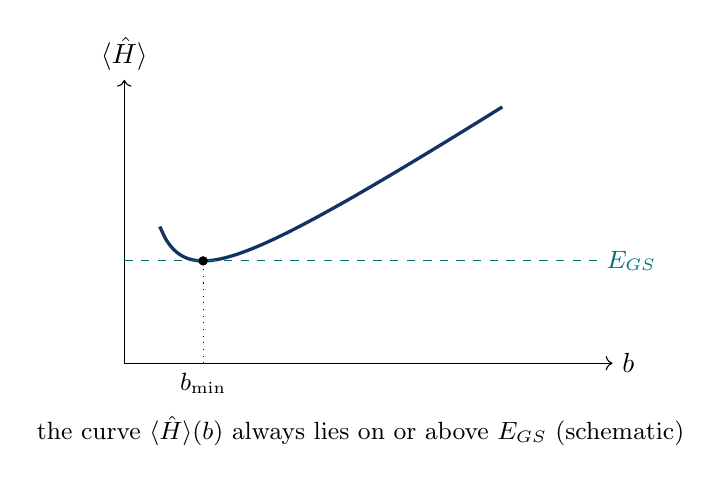
\begin{tikzpicture}[scale=1.0]
  \draw[->] (0,0) -- (6.2,0) node[right] {$b$};
  \draw[->] (0,0) -- (0,3.6) node[above] {$\langle\hat H\rangle$};
  \draw[very thick,primary,domain=0.45:4.8,samples=60,smooth] plot ({\x},{1.3*(\x+1/\x)/2});
  \draw[dashed,secondary] (0,1.3) -- (6,1.3) node[right] {\small $E_{GS}$};
  \fill (1,1.3) circle (0.06);
  \draw[dotted] (1,0) -- (1,1.3);
  \node[below] at (1,0) {\small $b_{\min}$};
  \node[below,align=center] at (3,-0.55) {\small the curve $\langle\hat H\rangle(b)$ always lies on or above $E_{GS}$ (schematic)};
\end{tikzpicture}
\end{center}

\subsection{Example: Delta-Function Potential}
\begin{prob}{Example: Variational Treatment of the Attractive Delta Potential}
$\hat H = -\dfrac{\hbar^2}{2m}\dfrac{d^2}{dx^2} - \alpha\delta(x)$, with exactly known $E_{GS} = -\dfrac{m\alpha^2}{2\hbar^2}$. Trial function $\psi(x) = A\exp(-bx^2)$ with $A = (2b/\pi)^{1/4}$.

\textbf{Kinetic energy} (same as before): $\langle T\rangle = \dfrac{\hbar^2b}{2m}$.\\
\textbf{Potential energy:}
\[
\langle V\rangle = -\alpha|A|^2\int_{-\infty}^{\infty}dx\,\delta(x)\,e^{-2bx^2} = -\alpha|A|^2 = -\alpha\sqrt{\frac{2b}{\pi}}
\]
\[
\langle\hat H\rangle = \frac{\hbar^2b}{2m} - \alpha\sqrt{\frac{2b}{\pi}}
\]
\textbf{Minimize:} $\dfrac{d}{db}\langle\hat H\rangle = \dfrac{\hbar^2}{2m} - \alpha\sqrt{\dfrac2\pi}\dfrac1{2\sqrt b} = 0 \Rightarrow \dfrac\alpha2\sqrt{\dfrac{2}{b\pi}} = \dfrac{\hbar^2}{2m}\Rightarrow b = \dfrac{2m^2\alpha^2}{\pi\hbar^4}$. Hence
\[
\boxed{\langle\hat H\rangle_{\min} = -\frac{m\alpha^2}{\pi\hbar^2} > E_{GS}}
\]
\textbf{*** Verification:} $-\dfrac{m\alpha^2}{\pi\hbar^2} = \dfrac2\pi E_{GS}\approx0.64\,E_{GS}$, which is higher (less negative) than $E_{GS}$ since $\pi>2$, so the upper-bound property holds. The exact ground state is $\psi=\sqrt\kappa\,e^{-\kappa|x|}$ with $\kappa=m\alpha/\hbar^2$; a Gaussian has the wrong cusp at $x=0$, which is why the energy is only about 64\% of the exact binding energy.
\end{prob}

\subsection{Ground State of Helium}
The helium atom has a nucleus of charge $+2e$ and two electrons at $\vec r_1,\vec r_2$, with $\vec r = \vec r_2-\vec r_1$ the separation.
\begin{center}
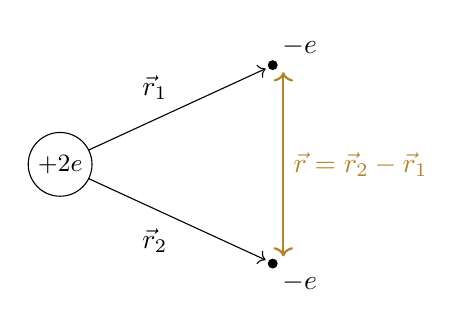
\begin{tikzpicture}[scale=0.9]
  \draw (0,0) circle (0.45); \node at (0,0) {\small $+2e$};
  \fill (3,1.4) circle (0.07); \node[above right] at (3,1.4) {$-e$};
  \fill (3,-1.4) circle (0.07); \node[below right] at (3,-1.4) {$-e$};
  \draw[->] (0.4,0.2) -- (2.9,1.35) node[midway,above left] {$\vec r_1$};
  \draw[->] (0.4,-0.2) -- (2.9,-1.35) node[midway,below left] {$\vec r_2$};
  \draw[<->,exframe,thick] (3.15,1.3) -- (3.15,-1.3) node[midway,right] {$\vec r=\vec r_2-\vec r_1$};
\end{tikzpicture}
\end{center}
\[
\hat H = -\frac{\hbar^2}{2m}\big(\nabla_1^2+\nabla_2^2\big) - \frac{e^2}{4\pi\varepsilon_0}\Big(\frac2{r_1}+\frac2{r_2}\Big) + \frac{e^2}{4\pi\varepsilon_0}\frac1{|\vec r_1-\vec r_2|}
\]
Experimentally the ground-state energy is $E_{GS} = -78.975\ \text{eV}\approx -79$ eV.

\begin{prob}{Ground State of Helium: Setup and Trial Function}
\textbf{Step 1: neglect the electron-electron interaction.} Then $\hat H = \hat h_1+\hat h_2$ with $\hat h_i = -\frac{\hbar^2}{2m}\nabla_i^2 - \frac{e^2}{4\pi\varepsilon_0}\frac2{r_i}$, and $\phi(\vec r_1,\vec r_2) = \psi_1(\vec r_1)\psi_2(\vec r_2)$ with $\hat h_i\psi_i = \varepsilon_i\psi_i$. Each $\hat h_i$ is a hydrogen-like Hamiltonian with nuclear charge $2e$, whose Bohr radius is $a_{He} = \dfrac{4\pi\varepsilon_0\hbar^2}{m\,2e\cdot e} = \dfrac{a_H}2$. Writing $a\equiv a_H$ and $E_H$ for the hydrogen ground-state energy,
\[
\psi^{H}_{100}(r) = \frac1{\sqrt{\pi a^3}}e^{-r/a}, \qquad \psi^{He^+}_{100}(r) = \sqrt{\frac{8}{\pi a^3}}\,e^{-2r/a}, \qquad E_H = -\frac{m}{2\hbar^2}\Big(\frac{e^2}{4\pi\varepsilon_0}\Big)^2\approx-13.6\ \text{eV}
\]
The energy of a hydrogen-like ion with charge $2e$ is $4E_H$, so $\varepsilon_1=\varepsilon_2=4E_H$:
\begin{gather*}
\phi(\vec r_1,\vec r_2) = \frac{8}{\pi a^3}\exp\Big[-\frac2a(r_1+r_2)\Big]\\
E = \varepsilon_1+\varepsilon_2 = 8E_H\approx-109\ \text{eV}\quad(\text{without } e^-e^-\text{ interaction})
\end{gather*}
\textbf{*** Study Note (sign of $E_H$):} The notebook writes $E_H=\frac{m}{2\hbar^2}\big(\frac{e^2}{4\pi\varepsilon_0}\big)^2$, but it uses $E_H$ as the (negative) hydrogen ground-state energy $-13.6$ eV (for example $8E_H=-109$ eV, $-\frac52E_H=+34$ eV). The explicit minus sign is written above.

\textbf{Step 2: use $\phi_0=\phi(\vec r_1,\vec r_2)$ as a trial wavefunction for the full $\hat H = \hat h_1+\hat h_2+\dfrac{e^2}{4\pi\varepsilon_0}\dfrac1{|\vec r_1-\vec r_2|}$.}
\[
\langle\phi_0|\hat H|\phi_0\rangle = \langle\phi_0|\hat h_1+\hat h_2|\phi_0\rangle + \frac{e^2}{4\pi\varepsilon_0}\Big\langle\phi_0\Big|\frac1{|\vec r_1-\vec r_2|}\Big|\phi_0\Big\rangle = 8E_H + V_{ee}
\]
\[
V_{ee} = \frac{e^2}{4\pi\varepsilon_0}\Big(\frac{8}{\pi a^3}\Big)^2\int\!\!\int\frac{\exp\!\big[-\frac4a(r_1+r_2)\big]}{|\vec r_1-\vec r_2|}\,d^3r_1\,d^3r_2
= \frac{e^2}{4\pi\varepsilon_0}\Big(\frac{8}{\pi a^3}\Big)^2\int e^{-4r_1/a}\,I_2(r_1)\,d^3r_1
\]
with the inner integral $I_2(r_1) = \displaystyle\int\frac{e^{-4r_2/a}}{|\vec r_1-\vec r_2|}\,d^3r_2$. Choose the $z_2$-axis along $\vec r_1$, so that $|\vec r_1-\vec r_2| = \sqrt{r_1^2+r_2^2-2r_1r_2\cos\theta_2}$.
\begin{center}
\begin{tikzpicture}[scale=0.9]
  \draw[->] (0,0) -- (0,3.2) node[above] {$z_2$};
  \draw[->] (0,0) -- (3.4,0) node[right] {$y_2$};
  \draw[->] (0,0) -- (-1.5,-1.0) node[below left] {$x_2$};
  \draw[->,thick,primary] (0,0) -- (0,2.3) node[right] {$\vec r_1$};
  \draw[->,thick,secondary] (0,0) -- (2.4,1.7) node[above right] {$\vec r_2$};
  \draw (0,0.7) arc (90:35:0.7);
  \node at (0.55,0.95) {\small $\theta_2$};
\end{tikzpicture}
\end{center}
\end{prob}

\begin{prob}{Ground State of Helium (continued): the Integral $V_{ee}$}
\textbf{Angular integral.} With $d^3r_2 = r_2^2\sin\theta_2\,dr_2\,d\theta_2\,d\varphi_2$ and the $\varphi_2$ integration giving $2\pi$:
\[
I_2 = 2\pi\int_0^\infty r_2^2e^{-4r_2/a}\,I_3\,dr_2, \qquad I_3 = \int_{-1}^{1}\frac{d(\cos\theta_2)}{\sqrt{r_1^2+r_2^2-2r_1r_2\cos\theta_2}} = \frac{1}{r_1r_2}\big(r_1+r_2-|r_1-r_2|\big)
\]
so that $I_3 = \dfrac{2}{r_1}$ for $r_1>r_2$ and $I_3 = \dfrac2{r_2}$ for $r_1<r_2$. Then
\[
I_2 = 4\pi\left[\frac1{r_1}\int_0^{r_1}e^{-4r_2/a}\,r_2^2\,dr_2 + \int_{r_1}^\infty e^{-4r_2/a}\,r_2\,dr_2\right]
= \frac{\pi a^3}{8r_1}\left[1 - \Big(1+\frac{2r_1}{a}\Big)e^{-4r_1/a}\right]
\]
\textbf{Radial integral.} With $d^3r_1 = 4\pi r_1^2dr_1$:
\[
V_{ee} = \frac{e^2}{4\pi\varepsilon_0}\Big(\frac8{\pi a^3}\Big)^2\,4\pi\,\frac{\pi a^3}{8}\int_0^\infty r_1\Big[e^{-4r_1/a} - \Big(1+\frac{2r_1}a\Big)e^{-8r_1/a}\Big]dr_1
\]
\textbf{*** Complete Solution:} The three elementary integrals are $\int_0^\infty r\,e^{-4r/a}dr = \frac{a^2}{16}$, $\int_0^\infty r\,e^{-8r/a}dr = \frac{a^2}{64}$ and $\frac2a\int_0^\infty r^2e^{-8r/a}dr = \frac{a^2}{128}$, so the bracket integral is $\frac{a^2}{16}-\frac{a^2}{64}-\frac{a^2}{128} = \frac{5a^2}{128}$. The prefactor is $\big(\frac{8}{\pi a^3}\big)^2\,4\pi\,\frac{\pi a^3}{8} = \frac{32}{a^3}$, hence
\begin{thm}{Electron-Electron Repulsion in the Trial State}
\[
V_{ee} = \frac{5}{4a}\Big(\frac{e^2}{4\pi\varepsilon_0}\Big) = -\frac52E_H \approx +34\ \text{eV}
\]
\[
\langle\hat H\rangle = 8E_H - \tfrac52E_H = (-109+34)\ \text{eV} = -75\ \text{eV} > E_{GS}
\]
\end{thm}
This is already within about 5\% of the experimental $-78.975$ eV.

\textbf{Even better: screening.} Each electron screens the nucleus from the other, so an electron effectively sees a charge smaller than $+2e$. Take a nuclear charge $Z$ as the \textbf{variational parameter}:
\[
\psi(\vec r_1,\vec r_2) = \frac{Z^3}{\pi a^3}\exp\Big[-\frac Za(r_1+r_2)\Big]
\]
\textbf{*** Study Note:} The notebook writes the prefactor as $Z^3/8a^3$; the normalized prefactor is $Z^3/(\pi a^3)$ (which reduces to $8/\pi a^3$ at $Z=2$, as above).

\textbf{*** Complete Solution (the $Z$-dependence):} With hydrogen-like expectation values for charge $Z$, $\langle T\rangle = -Z^2E_H$ per electron, $\langle 1/r\rangle=Z/a$, and the true attraction to charge $2e$:
\[
\langle T\rangle_{\text{tot}} = -2Z^2E_H, \qquad \langle V_{Ne}\rangle_{\text{tot}} = +8ZE_H, \qquad \langle V_{ee}\rangle = \frac{5Z}{4a}\frac{e^2}{4\pi\varepsilon_0} = -\frac54ZE_H
\]
\[
\langle\hat H\rangle = \Big[2Z^2 - 4(Z-2)Z - \tfrac54Z\Big]E_H = \Big[-2Z^2+\tfrac{27}{4}Z\Big]E_H
\]
(The form $2Z^2-4(Z-2)Z=-2Z^2+8Z$ is the sum of the kinetic and nuclear-attraction terms.) At $Z=2$ this gives $5.5E_H=-74.8$ eV, matching the result above. Minimize with $E_H<0$:
\[
\frac{d}{dZ}\langle\hat H\rangle = 0 \;\Rightarrow\; -4Z+\tfrac{27}4=0 \;\Rightarrow\; \boxed{Z=\tfrac{27}{16}=1.69}, \qquad \boxed{\langle\hat H\rangle = -77.5\ \text{eV}}
\]
\textbf{*** Verification:} $\big(-2Z^2+\frac{27}4Z\big)\big|_{Z=27/16} = \frac{729}{128}=5.69$, and $5.69\times(-13.6)=-77.5$ eV, still above (less negative than) the experimental $-78.975$ eV, within about 2\%. $Z_{\text{eff}}=1.69<2$ is the screening effect.
\end{prob}

\textbf{*** Common mistakes:} (a) forgetting to normalize the trial function, (b) using a trial function that does not satisfy the boundary conditions of the problem, (c) minimizing the wrong quantity (minimize $\langle\hat H\rangle$, not $\langle T\rangle$), (d) interpreting the minimum as an exact energy: it is only an \textit{upper bound}, (e) confusing $E_H$ (negative) with the Rydberg energy $+13.6$ eV.

%==============================================================================
\section{The WKB Approximation}
%==============================================================================

\subsection{Idea and Setting}
The \textbf{WKB (Wentzel, Kramers, Brillouin) approximation} is applicable to one-dimensional systems. Start from the 1D Schr\"odinger equation
\[
-\frac{\hbar^2}{2m}\frac{d^2\psi}{dx^2} + V(x)\psi(x) = E\psi(x)
\]
\textbf{Constant potential} ($E>V$, bound-state-type problem): with $\kappa^2 = (E-V)\dfrac{2m}{\hbar^2}$ we have $\dfrac{d^2\psi}{dx^2} = -\kappa^2\psi$ and
\[
\psi(x) = A\,e^{\pm i\kappa x}, \qquad \kappa = \sqrt{\frac{2m}{\hbar^2}(E-V)}, \qquad \text{wavelength } \lambda = \frac{2\pi}{\kappa}
\]
\textbf{Classically forbidden region} ($E<V$, scattering problem): $\psi(x) = A\,e^{\pm\chi x}$ with $\chi = \dfrac1\hbar\sqrt{2m(V-E)}$, and $1/\chi$ is the length scale of the decay.

For a potential that varies slowly compared with the wavelength $\lambda$, the logic of WKB is: \textit{rapid oscillations modulated by a gradual variation of the amplitude and of the phase}. The approximation breaks down at $E=V$, the \textbf{classical turning points}, where $p(x)=0$.

\begin{center}
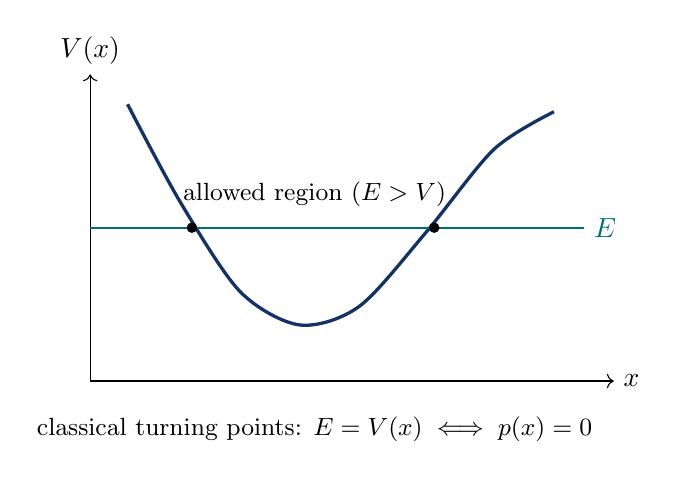
\begin{tikzpicture}[scale=0.95]
  \draw[->] (0,0) -- (7,0) node[right] {$x$};
  \draw[->] (0,0) -- (0,4.1) node[above] {$V(x)$};
  \draw[very thick,primary] plot[smooth] coordinates {(0.5,3.7) (1.2,2.4) (2,1.2) (2.8,0.75) (3.6,1.0) (4.5,2.0) (5.4,3.1) (6.2,3.6)};
  \draw[secondary,thick] (0,2.05) -- (6.6,2.05) node[right] {$E$};
  \fill (1.36,2.05) circle (0.07);
  \fill (4.6,2.05) circle (0.07);
  \node[below,align=center] at (3,-0.35) {\small classical turning points: $E=V(x)\iff p(x)=0$};
  \node at (3,2.5) {\small allowed region ($E>V$)};
\end{tikzpicture}
\end{center}
With the classical momentum
\[
\frac{\hat p^2}{2m}\psi = -\frac{\hbar^2}{2m}\frac{d^2\psi}{dx^2} \;\Rightarrow\; \frac{d^2\psi}{dx^2} = -\frac1{\hbar^2}\hat p^2\psi, \qquad E = \frac{p^2}{2m}+V(x)\;\Rightarrow\; p(x) = \sqrt{2m\big(E-V(x)\big)}
\]

\subsection{\texorpdfstring{Derivation for $E>V$}{Derivation for E>V} (Classically Allowed Region)}
Try $\psi(x) = A(x)\,e^{i\phi(x)}$ with real $A$ and $\phi$. Then
\begin{align*}
\frac{d\psi}{dx} &= \big[A'(x) + iA(x)\phi'(x)\big]e^{i\phi(x)}\\
\frac{d^2\psi}{dx^2} &= \Big[A'' + 2iA'\phi' + iA\phi'' - A(\phi')^2\Big]e^{i\phi(x)}
\end{align*}
Substituting into $\psi'' = -\frac{p^2}{\hbar^2}\psi$ and cancelling $e^{i\phi}$:
\[
-\frac{p^2}{\hbar^2}A = A'' + 2iA'\phi' + iA\phi'' - A(\phi')^2
\]
Equating the real and the imaginary parts:
\begin{align}
A'' - A(\phi')^2 &= -\frac{p^2}{\hbar^2}A \tag{i}\\
2A'\phi' + A\phi'' &= 0 \tag{ii}
\end{align}
Multiplying (ii) by $A$ gives $2AA'\phi' + A^2\phi'' = (A^2\phi')' = 0$, so $A^2\phi' = c^2$ is constant:
\[
A = \frac{c}{\sqrt{\phi'}} \qquad (c\ \text{a real constant})
\]
For a slowly varying potential assume $A''\approx0$. Equation (i) then becomes $(\phi')^2 = p^2/\hbar^2$, i.e.\ $\dfrac{d\phi}{dx} = \pm\dfrac p\hbar$:
\[
\phi(x) = \pm\frac1\hbar\int p(x)\,dx
\]
\begin{thm}{WKB Wavefunction}
\textbf{Allowed region} ($E>V$):
\[
\psi_{\text{WKB}}(x) = \frac{c}{\sqrt{p(x)}}\exp\Big[\pm\frac i\hbar\int p(x)\,dx\Big], \qquad |\psi_{\text{WKB}}(x)|^2 = \frac{c^2}{p(x)}
\]
\textbf{Forbidden region} ($E<V$, $|p| = \sqrt{2m(V-E)}$):
\[
\psi_{\text{WKB}}(x) = \frac{c}{\sqrt{|p(x)|}}\exp\Big[\pm\frac1\hbar\int|p(x)|\,dx\Big]
\]
\end{thm}
The probability of finding the particle at $x$ is inversely proportional to its momentum, exactly as in classical mechanics (it spends more time where it moves slowly). WKB is therefore also called the \textbf{semi-classical approximation}.

\textbf{*** Intuition:} The phase $\frac1\hbar\int p\,dx$ is the accumulated de Broglie phase (the local wave number times distance); the amplitude $1/\sqrt p$ keeps the probability flux $\propto|\psi|^2p$ constant.

\textbf{*** Study Note (validity):} From (i), $A''/A = (\phi')^2 - p^2/\hbar^2$. Dropping $A''$ is justified if $|A''/A|\ll p^2/\hbar^2$, which for $A\propto p^{-1/2}$ amounts to the de Broglie wavelength $\lambda_{dB}=2\pi\hbar/p$ changing little over one wavelength, $|d\lambda_{dB}/dx|\ll1$, i.e.\ $\hbar|p'|\ll p^2$. This fails at the turning points ($p\to0$), where the WKB wavefunction blows up as $1/\sqrt p$; the connection formulas of Section~\ref{ap:sec:conn} repair this.

\textbf{*** Memory Rule:} Allowed region: oscillating with phase $\frac1\hbar\int p\,dx$. Forbidden region: real exponential with $\frac1\hbar\int|p|\,dx$. Both carry the prefactor $1/\sqrt{|p|}$.

\subsection{Bound States: Particle in a Well with a Slowly Varying Floor}
\begin{prob}{Example: Infinite Well with a Non-Constant Bottom}
\begin{center}
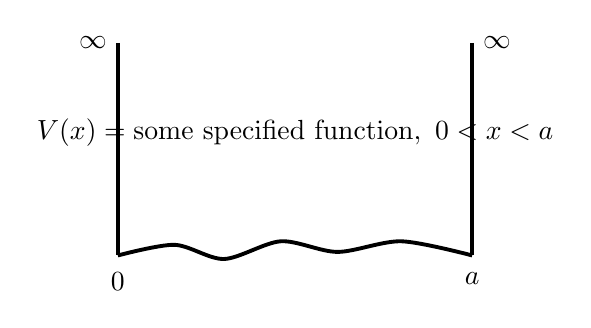
\begin{tikzpicture}[scale=0.9]
  \draw[line width=1.4pt] (0,3) -- (0,0);
  \draw[line width=1.4pt] (5,3) -- (5,0);
  \draw[line width=1.4pt] plot[smooth] coordinates {(0,0) (0.8,0.15) (1.5,-0.05) (2.3,0.2) (3.1,0.05) (4,0.2) (5,0)};
  \node[below] at (0,-0.1) {$0$}; \node[below] at (5,-0.1) {$a$};
  \node at (-0.35,3) {$\infty$}; \node at (5.35,3) {$\infty$};
  \node[above,align=center] at (2.5,1.4) {$V(x)=\text{some specified function},\ 0<x<a$};
\end{tikzpicture}
\end{center}
Inside the well $E>V(x)$ and, since the solution may be written with real functions,
\begin{gather*}
\psi(x)\simeq\frac1{\sqrt{p(x)}}\Big[C_+e^{i\phi(x)} + C_-e^{-i\phi(x)}\Big]
\quad\text{or}\quad
\psi(x)\simeq\frac{1}{\sqrt{p(x)}}\Big[C_1\sin\phi(x) + C_2\cos\phi(x)\Big]\\
\phi(x) = \frac1\hbar\int_0^xp(x')\,dx'
\end{gather*}
with $\phi(0)=0$. Boundary conditions: $\psi(0)=0\Rightarrow C_2=0$, so $\psi(x) = \frac{C_1}{\sqrt{p(x)}}\sin\phi(x)$; and $\psi(a)=0\Rightarrow\sin\phi(a)=0$, i.e.\ $\phi(a)=n\pi$ $(n=1,2,\ldots)$:
\[
\boxed{\int_0^ap(x)\,dx = n\pi\hbar}
\]
\textbf{Check with $V(x)=0$:} $p=\sqrt{2mE}$ is constant, so $\sqrt{2mE}\,a = n\pi\hbar$ and
\[
E_n = \frac{n^2\pi^2\hbar^2}{2ma^2}\qquad(\text{particle in a box})
\]
which is exact.
\end{prob}
\textbf{*** Study Note:} The rule $\int p\,dx = n\pi\hbar$ for two hard walls is the Bohr--Sommerfeld condition: the phase accumulated across the well equals $n\pi$, so that a half-integer number of wavelengths fits.

\subsection{Tunneling}
\begin{prob}{Example: Tunneling Through a Barrier}
A particle with energy $E$ is incident from the left on a barrier occupying $0<x<a$, where $V>E$.
\begin{center}
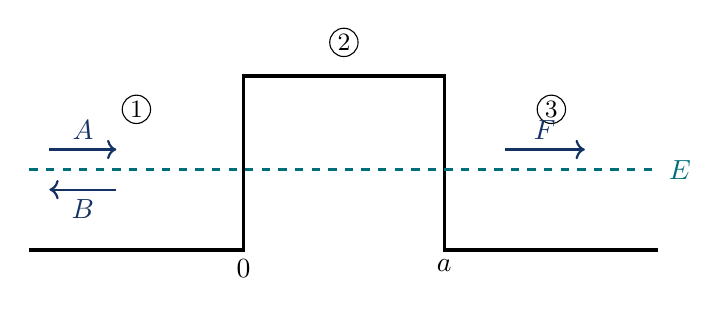
\begin{tikzpicture}[scale=0.85]
  \draw[line width=1.2pt] (-3.2,0) -- (0,0) -- (0,2.6) -- (3,2.6) -- (3,0) -- (6.2,0);
  \draw[dashed,secondary,thick] (-3.2,1.2) -- (6.2,1.2) node[right] {$E$};
  \node[below] at (0,0) {$0$}; \node[below] at (3,0) {$a$};
  \node[draw,circle,inner sep=1pt] at (-1.6,2.1) {\small 1};
  \node[draw,circle,inner sep=1pt] at (1.5,3.1) {\small 2};
  \node[draw,circle,inner sep=1pt] at (4.6,2.1) {\small 3};
  \draw[->,thick,primary] (-2.9,1.5) -- (-1.9,1.5) node[midway,above] {$A$};
  \draw[<-,thick,primary] (-2.9,0.9) -- (-1.9,0.9) node[midway,below] {$B$};
  \draw[->,thick,primary] (3.9,1.5) -- (5.1,1.5) node[midway,above] {$F$};
\end{tikzpicture}
\end{center}
\textbf{Region 1} ($x<0$): $\psi(x) = Ae^{ikx}+Be^{-ikx}$, with $k=\sqrt{2mE/\hbar^2}$. \textbf{Region 3} ($x>a$): $\psi(x) = Fe^{ikx}$. The transmission probability is
\[
T = \frac{|F|^2}{|A|^2}
\]
\textbf{Region 2} (tunneling region, $0<x\le a$):
\[
\psi_{\text{WKB}}(x) = \frac{C}{\sqrt{|p(x)|}}\exp\Big[\frac1\hbar\int_0^x|p(x')|\,dx'\Big] + \frac{D}{\sqrt{|p(x)|}}\exp\Big[-\frac1\hbar\int_0^x|p(x')|\,dx'\Big]
\]
\begin{center}
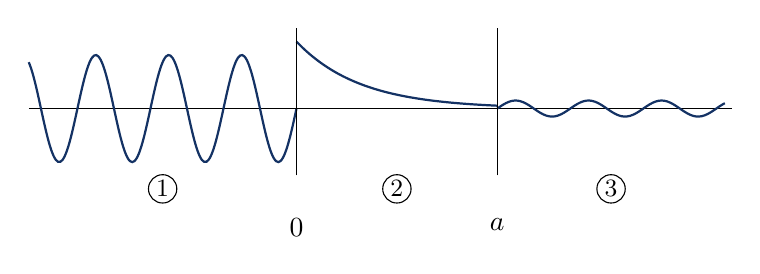
\begin{tikzpicture}[scale=0.85]
  \draw[thin] (-4,0) -- (6.5,0);
  \draw[thick,primary] plot[domain=-4:0,samples=120,smooth] (\x,{0.8*sin(\x*330)});
  \draw[thick,primary] plot[domain=0:3,samples=40,smooth] (\x,{1.0*exp(-1.05*\x)});
  \draw[thick,primary] plot[domain=3:6.4,samples=80,smooth] (\x,{0.12*sin((\x-3)*330)});
  \draw (0,-1) -- (0,1.2); \draw (3,-1) -- (3,1.2);
  \node[draw,circle,inner sep=1pt] at (-2,-1.2) {\small 1};
  \node[draw,circle,inner sep=1pt] at (1.5,-1.2) {\small 2};
  \node[draw,circle,inner sep=1pt] at (4.7,-1.2) {\small 3};
  \node[below] at (0,-1.5) {$0$}; \node[below] at (3,-1.5) {$a$};
\end{tikzpicture}
\end{center}
Only the decaying exponential is attached to the outgoing wave, so the amplitude ratio is controlled by the decay across the barrier,
\[
\frac{|F|}{|A|}\sim\exp\Big[-\frac1\hbar\int_0^a|p(x')|\,dx'\Big]\;\Rightarrow\;\frac{|F|^2}{|A|^2}\sim e^{-2\gamma}=T
\]
\end{prob}
\begin{thm}{WKB Tunneling Probability}
\[
T = \Big|\frac FA\Big|^2 = e^{-2\gamma}, \qquad \gamma = \frac1\hbar\int_0^a|p(x)|\,dx
\]
\end{thm}
\textbf{*** Intuition:} $e^{-\gamma}$ is the amplitude suppression, accumulated slice by slice, across the barrier of the decay rate $|p|/\hbar$. The result is reliable in its exponent when $\gamma\gg1$ (a thick or high barrier); the $O(1)$ prefactor is ignored.

\subsection{Application: \texorpdfstring{$\alpha$}{alpha}-Decay (Gamow)}
Let $Ze$ be the nuclear charge (of the daughter nucleus) and $2e$ the charge of the $\alpha$ particle (He$^{2+}$). For example $^{239}_{\ 94}\text{Pu}\to{}^{235}_{\ 92}\text{U}+{}^{4}_{2}\text{He}$.
\begin{center}
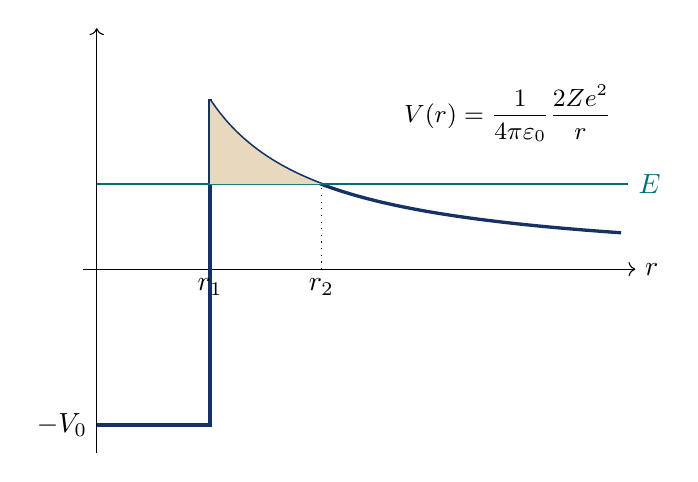
\begin{tikzpicture}[scale=0.9]
  \draw[->] (0,-2.6) -- (0,3.4); \draw[->] (-0.2,0) -- (7.6,0) node[right] {$r$};
  \draw[very thick,primary] (0,-2.2) -- (1.6,-2.2) -- (1.6,2.4);
  \draw[very thick,primary,domain=1.6:7.4,samples=60,smooth] plot (\x,{3.8/\x});
  \draw[secondary,thick] (0,1.2) -- (7.5,1.2) node[right] {$E$};
  \fill[exframe!30] (1.6,1.2) -- (1.6,2.375) -- plot[domain=1.6:3.1667,samples=40] (\x,{3.8/\x}) -- cycle;
  \node[left] at (0,-2.2) {$-V_0$};
  \node[below] at (1.6,0) {$r_1$}; \node[below] at (3.17,0) {$r_2$};
  \draw[dotted] (3.17,0) -- (3.17,1.2);
  \node[right,align=left] at (4.2,2.2) {\small $V(r)=\dfrac{1}{4\pi\varepsilon_0}\dfrac{2Ze^2}{r}$};
\end{tikzpicture}
\end{center}
The $\alpha$ particle with energy $E$ sits in the attractive nuclear well ($r<r_1$) and must tunnel through the Coulomb barrier from $r_1$ to the exit point $r_2$, where
\[
E = V(r_2) = \frac1{4\pi\varepsilon_0}\frac{2Ze^2}{r_2}
\]
\begin{align*}
\gamma &= \frac1\hbar\int_{r_1}^{r_2}|p(r)|\,dr = \frac1\hbar\int_{r_1}^{r_2}\sqrt{2m\Big(\frac1{4\pi\varepsilon_0}\frac{2Ze^2}{r}-E\Big)}\,dr = \frac1\hbar\int_{r_1}^{r_2}dr\sqrt{2mE\Big(\frac{r_2}{r}-1\Big)}
\end{align*}
Substitute $r = r_2\sin^2u$ (see the completed integral below) to get the final answer
\begin{thm}{Gamow Exponent}
\[
\gamma = \frac{\sqrt{2mE}}{\hbar}\left[r_2\Big(\frac\pi2-\sin^{-1}\sqrt{\frac{r_1}{r_2}}\Big) - \sqrt{r_1(r_2-r_1)}\right]
\]
For $r_1\ll r_2$:
\[
\gamma\simeq\frac{\sqrt{2mE}}{\hbar}\Big[\frac\pi2r_2 - 2\sqrt{r_1r_2}\Big]
\]
Eliminating $r_2 = 2Ze^2/(4\pi\varepsilon_0E)$ in terms of $E$:
\begin{gather*}
\gamma\simeq k_1\frac{Z}{\sqrt E} - k_2\sqrt{Zr_1}\\
k_1 = \Big(\frac{e^2}{4\pi\varepsilon_0}\Big)\pi\frac{\sqrt{2m}}\hbar\simeq1.98\ \text{MeV}^{1/2},\qquad
k_2 = \Big(\frac{e^2}{4\pi\varepsilon_0}\Big)^{1/2}\frac{4\sqrt m}{\hbar}\simeq1.485\ \text{fm}^{-1/2}
\end{gather*}
\end{thm}
Here $m$ is the mass of the $\alpha$ particle.

\begin{prob}{$\alpha$-Decay (continued): Completed Integral and Lifetime}
\textbf{*** Complete Solution (the integral):} With $r=r_2\sin^2u$, $dr = 2r_2\sin u\cos u\,du$ and $\sqrt{r_2/r-1}=\cot u$:
\[
\int_{r_1}^{r_2}\sqrt{\frac{r_2}r-1}\,dr = 2r_2\int_{u_1}^{\pi/2}\cos^2u\,du = r_2\Big[u+\sin u\cos u\Big]_{u_1}^{\pi/2}, \qquad \sin u_1 = \sqrt{\frac{r_1}{r_2}}
\]
which equals $r_2\big(\frac\pi2-u_1\big)-\sqrt{r_1(r_2-r_1)}$, since $r_2\sin u_1\cos u_1 = \sqrt{r_1(r_2-r_1)}$. (The notebook writes $r=r_2\sin u$; the substitution that works is $r=r_2\sin^2u$.) For $r_1\ll r_2$, $\sin^{-1}\sqrt{r_1/r_2}\approx\sqrt{r_1/r_2}$ and the bracket becomes $\frac\pi2r_2-\sqrt{r_1r_2}-\sqrt{r_1r_2}$.

\textbf{*** Complete Solution (eliminating $r_2$):} $\dfrac{\sqrt{2mE}}\hbar\dfrac\pi2r_2 = \dfrac{\pi\sqrt{2m}}{\hbar}\dfrac{Ze^2}{4\pi\varepsilon_0}\dfrac1{\sqrt E} = k_1\dfrac Z{\sqrt E}$ and $\dfrac{\sqrt{2mE}}\hbar2\sqrt{r_1r_2} = \dfrac{4\sqrt m}{\hbar}\Big(\dfrac{e^2}{4\pi\varepsilon_0}\Big)^{1/2}\sqrt{Zr_1} = k_2\sqrt{Zr_1}$. \checkmark

\textbf{Lifetime.} The $\alpha$ particle rattles back and forth inside the nucleus with speed $v$, hitting the barrier at the \textbf{rattling frequency} $\dfrac v{2r_1}$. Each hit has probability $e^{-2\gamma}$ of escape, so
\[
\text{Probability of emission per unit time} = \frac{v}{2r_1}\,e^{-2\gamma}
\]
\textbf{*** Complete Solution (lifetime):} The lifetime is $\tau = \dfrac{2r_1}{v}\,e^{2\gamma}$, hence $\ln\tau\simeq\text{const}+2k_1\dfrac{Z}{\sqrt E}$: a small increase in $1/\sqrt E$ (lower energy) changes the lifetime by many orders of magnitude (Geiger--Nuttall law).

\begin{center}
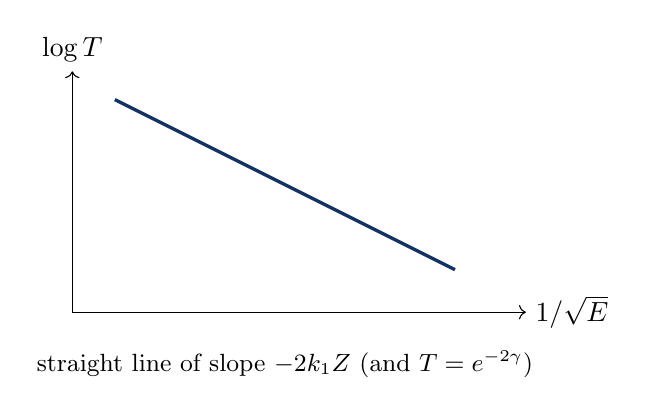
\begin{tikzpicture}[scale=0.9]
  \draw[->] (0,0) -- (6.4,0) node[right] {$1/\sqrt E$};
  \draw[->] (0,0) -- (0,3.4) node[above] {$\log T$};
  \draw[very thick,primary] (0.6,3.0) -- (5.4,0.6);
  \node[below,align=center] at (3,-0.4) {\small straight line of slope $-2k_1Z$ (and $T=e^{-2\gamma}$)};
\end{tikzpicture}
\end{center}
\textbf{*** Study Note:} The notebook's straight line is drawn decreasing in $1/\sqrt E$; this is the plot of $\log$ of the transmission (decay rate) $T=e^{-2\gamma}$, whose slope is $-2k_1Z$. The lifetime $\tau$ has the opposite (positive) slope.
\end{prob}

\subsection{The Connection Formulas}\label{ap:sec:conn}
Near a classical turning point WKB fails, but the potential is nearly \textit{linear} there, and for a linear potential the Schr\"odinger equation is solved exactly by Airy functions. Matching the Airy solution to WKB on both sides of the turning point gives the connection formulas.

\begin{center}
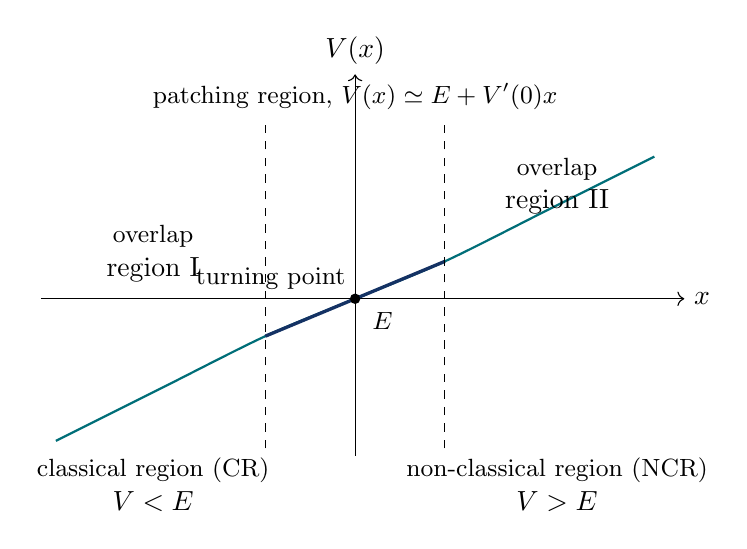
\begin{tikzpicture}[scale=0.95]
  \draw[->] (-4.2,0) -- (4.4,0) node[right] {$x$};
  \draw[->] (0,-2.1) -- (0,3.0) node[above] {$V(x)$};
  \draw[thick,secondary] plot[smooth] coordinates {(-4,-1.9) (-2.6,-1.2) (-1.2,-0.5) (0,0) (1.2,0.5) (2.6,1.2) (4,1.9)};
  \draw[very thick,primary] (-1.2,-0.5) -- (1.2,0.5);
  \draw[dashed] (-1.2,-2.0) -- (-1.2,2.4);
  \draw[dashed] (1.2,-2.0) -- (1.2,2.4);
  \node[above] at (0,2.4) {\small patching region, $V(x)\simeq E+V'(0)x$};
  \node[below right] at (0.1,-0.05) {\small $E$};
  \node[below,align=center] at (-2.7,-2.0) {\small classical region (CR)\\ $V<E$};
  \node[below,align=center] at (2.7,-2.0) {\small non-classical region (NCR)\\ $V>E$};
  \node[above,align=center] at (-2.7,0.1) {\small overlap\\ region I};
  \node[above,align=center] at (2.7,1.0) {\small overlap\\ region II};
  \fill (0,0) circle (0.07);
  \node[above left] at (0,0) {\small turning point};
\end{tikzpicture}
\end{center}
For $x<0$ (classical region) and $x>0$ (forbidden region) the WKB solutions are
\begin{align}
\psi(x)&\simeq\frac1{\sqrt{p(x)}}\Big[B\exp\Big(\frac i\hbar\int_x^0p(x')dx'\Big) + C\exp\Big(-\frac i\hbar\int_x^0p(x')dx'\Big)\Big]\qquad(x<0)\tag{A}\\
\psi(x)&\simeq\frac1{\sqrt{|p(x)|}}\,D\exp\Big\{-\frac1\hbar\int_0^x|p(x')|dx'\Big\}\qquad(x>0)\tag{B}
\end{align}
\textbf{Patching region.} Near the origin $V(x)\simeq E+V'(0)x$ (with $V'(0)>0$). The Schr\"odinger equation for the patching wavefunction $\psi_p$ is
\[
-\frac{\hbar^2}{2m}\frac{d^2\psi_p}{dx^2} + \big(E+V'(0)x\big)\psi_p = E\psi_p \;\Rightarrow\; \frac{d^2\psi_p}{dx^2} = \frac{2m}{\hbar^2}V'(0)\,x\,\psi_p = \alpha^3x\,\psi_p,\qquad \alpha^3 = \frac{2mV'(0)}{\hbar^2}
\]
With $z=\alpha x$ this becomes the \textbf{Airy differential equation}
\begin{thm}{Airy Equation and Its Solution}
\[
\frac{d^2\psi_p}{dz^2} = z\,\psi_p, \qquad \psi_p(x) = a\,\mathrm{Ai}(\alpha x) + b\,\mathrm{Bi}(\alpha x)
\]
Asymptotic forms: for large positive $z$,
\[
\mathrm{Ai}(z)\sim\frac1{2\sqrt\pi}\frac1{z^{1/4}}e^{-\frac23z^{3/2}}, \qquad \mathrm{Bi}(z)\sim\frac1{\sqrt\pi}\frac1{z^{1/4}}e^{+\frac23z^{3/2}}
\]
and for large negative $z$,
\[
\mathrm{Ai}(z)\sim\frac1{\sqrt\pi}\frac1{(-z)^{1/4}}\sin\Big(\frac23(-z)^{3/2}+\frac\pi4\Big)
\]
\end{thm}
In the patching region the momentum is $p(x)=\sqrt{2m(E-E-V'(0)x)} = \sqrt{-2mV'(0)x}$, i.e.
\[
p(x) = \hbar\alpha^{3/2}\sqrt{-x}
\]
\textbf{Overlap region II} ($x>0$). Here $\int_0^x|p|\,dx' = \hbar\alpha^{3/2}\int_0^x\sqrt{x'}\,dx' = \frac23\hbar(\alpha x)^{3/2}$, so (B) becomes
\[
\psi(x)\simeq\frac{D}{\sqrt\hbar\,\alpha^{3/4}x^{1/4}}\exp\Big(-\frac23(\alpha x)^{3/2}\Big) \tag{C}
\]
whereas the asymptotic Airy solution is
\[
\psi_p(x) = \frac{a}{2\sqrt\pi(\alpha x)^{1/4}}\exp\Big(-\frac23(\alpha x)^{3/2}\Big) + \frac{b}{\sqrt\pi(\alpha x)^{1/4}}\exp\Big(\frac23(\alpha x)^{3/2}\Big) \tag{C$'$}
\]
Comparing (C) and (C$'$): $b=0$ (no growing exponential) and
\[
\boxed{a = \sqrt{\frac{4\pi}{\alpha\hbar}}\,D}
\]
\textbf{Overlap region I} ($x<0$). Now $\int_x^0p\,dx' = \frac23\hbar(-\alpha x)^{3/2}$, and (A) becomes
\[
\psi(x)\simeq\frac{1}{\sqrt\hbar\,\alpha^{3/4}(-x)^{1/4}}\Big[B\exp\Big\{i\tfrac23(-\alpha x)^{3/2}\Big\} + C\exp\Big\{-i\tfrac23(-\alpha x)^{3/2}\Big\}\Big] \tag{D}
\]
The Airy solution with $b=0$ and the large negative $z$ asymptotics (the notebook calls it the ``small $z$'' form) is
\begin{align*}
\psi_p(x) &= \frac{a}{\sqrt\pi(-\alpha x)^{1/4}}\sin\Big[\frac23(-\alpha x)^{3/2}+\frac\pi4\Big]\\
&= \frac{a}{\sqrt\pi(-\alpha x)^{1/4}}\frac1{2i}\Big[e^{i\pi/4}e^{i\frac23(-\alpha x)^{3/2}} - e^{-i\pi/4}e^{-i\frac23(-\alpha x)^{3/2}}\Big] \tag{D$''$}
\end{align*}
Matching (D) and (D$''$):
\[
\frac{B}{\sqrt{\hbar\alpha}} = \frac a{2i\sqrt\pi}e^{i\pi/4}, \qquad \frac C{\sqrt{\hbar\alpha}} = -\frac a{2i\sqrt\pi}e^{-i\pi/4}
\]
Solving with $a=\sqrt{4\pi/\hbar\alpha}\,D$:
\begin{thm}{Connection Formulas}
\[
B = -i\,e^{i\pi/4}\,D, \qquad C = i\,e^{-i\pi/4}\,D
\]
\end{thm}
Inserting these into (A) the two exponentials combine into a sine:
\[
\psi(x)\simeq\frac D{\sqrt{p(x)}}\Big[-ie^{i\pi/4}e^{\frac i\hbar\int_x^0p\,dx'} + ie^{-i\pi/4}e^{-\frac i\hbar\int_x^0p\,dx'}\Big]
\]
\begin{thm}{Wavefunctions at a Turning Point}
\textbf{Left side, classical turning point at $x=0$ (allowed region $x<0$):}
\begin{gather*}
\psi(x)\simeq\frac{2D}{\sqrt{p(x)}}\sin\Big[\frac1\hbar\int_x^0p(x')\,dx' + \frac\pi4\Big]\quad(x<0)\\
\psi(x)\simeq\frac D{\sqrt{|p(x)|}}\exp\Big[-\frac1\hbar\int_0^x|p(x')|\,dx'\Big]\quad(x>0)
\end{gather*}
\textbf{Right-hand turning point at $x=x_2$ (allowed region $x<x_2$):}
\begin{gather*}
\psi(x)\simeq\frac{2D}{\sqrt{p(x)}}\sin\Big[\frac1\hbar\int_x^{x_2}p(x')\,dx' + \frac\pi4\Big]\quad(x<x_2)\\
\psi(x)\simeq\frac D{\sqrt{|p(x)|}}\exp\Big[-\frac1\hbar\int_{x_2}^x|p(x')|\,dx'\Big]\quad(x>x_2)
\end{gather*}
\end{thm}
\textbf{*** Intuition:} A decaying exponential in the forbidden region connects to a sine with a phase offset $\pi/4$ in the allowed region, with amplitude $2D$ against $D$ (the standing wave is the superposition of an incident and a reflected wave of equal strength). The offset $\pi/4$ is a built-in phase shift of the reflection at a soft turning point (compare a hard wall, where the offset is $0$).

\textbf{*** Study Note:} These formulas apply only when the forbidden-region solution is purely \textit{decaying} (the case $b=0$ used above). Which sign of $V'(0)$ occurs decides on which side the allowed region lies; the second set above is the mirror image (decreasing potential).

\textbf{*** Verification:} Combining $-ie^{i\pi/4}e^{i\theta}+ie^{-i\pi/4}e^{-i\theta} = -i\big(e^{i(\theta+\pi/4)}-e^{-i(\theta+\pi/4)}\big) = 2\sin(\theta+\pi/4)$ with $\theta=\frac1\hbar\int_x^0p\,dx'$ reproduces the boxed sine. \checkmark

\subsection{Quantization with Turning Points}
\begin{prob}{Potential Well with One Vertical Wall}
\begin{center}
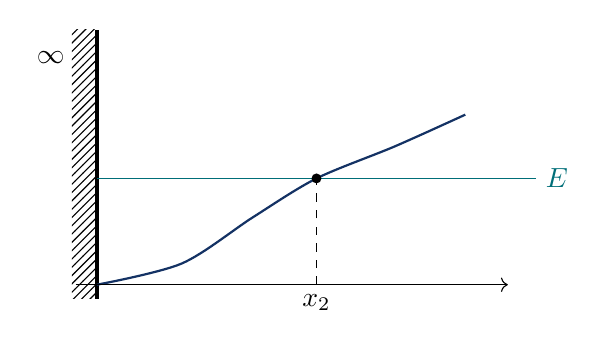
\begin{tikzpicture}[scale=0.9]
  \fill[pattern=north east lines] (-0.35,-0.2) rectangle (0,3.6);
  \draw[line width=1.4pt] (0,-0.2) -- (0,3.6);
  \node at (-0.65,3.2) {$\infty$};
  \draw[thick,primary] plot[smooth] coordinates {(0,0) (1.2,0.3) (2.2,0.95) (3.1,1.5) (4.2,1.95) (5.2,2.4)};
  \draw[secondary] (0,1.5) -- (6.2,1.5) node[right] {$E$};
  \fill (3.1,1.5) circle (0.07);
  \draw[dashed] (3.1,0) -- (3.1,1.5);
  \draw[->] (-0.3,0) -- (5.8,0);
  \node[below] at (3.1,0) {$x_2$};
\end{tikzpicture}
\end{center}
For $x<x_2$ the WKB wavefunction is
\[
\psi(x)\simeq\frac{2D}{\sqrt{p(x)}}\sin\Big[\frac1\hbar\int_x^{x_2}p(x')\,dx'+\frac\pi4\Big]
\]
The wall imposes $\psi(0)=0$:
\[
\sin\Big[\frac1\hbar\int_0^{x_2}p(x')\,dx'+\frac\pi4\Big]=0\;\Rightarrow\;\frac1\hbar\int_0^{x_2}p(x')\,dx'+\frac\pi4 = n\pi
\]
\[
\boxed{\int_0^{x_2}p(x')\,dx' = \Big(n-\frac14\Big)\pi\hbar\qquad(n=1,2,3,\ldots)}
\]
\end{prob}

\begin{prob}{Example: Half-Harmonic Oscillator}
\begin{center}
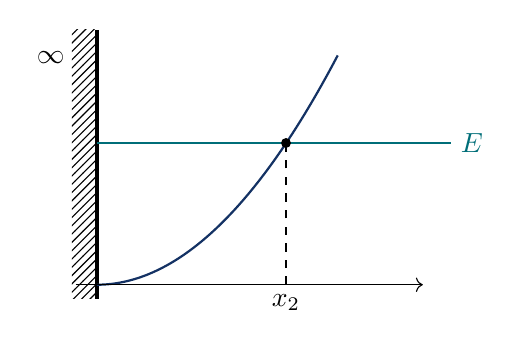
\begin{tikzpicture}[scale=0.9]
  \fill[pattern=north east lines] (-0.35,-0.2) rectangle (0,3.6);
  \draw[line width=1.4pt] (0,-0.2) -- (0,3.6);
  \node at (-0.65,3.2) {$\infty$};
  \draw[thick,primary,domain=0:3.4,samples=50,smooth] plot (\x,{0.28*\x*\x});
  \draw[secondary] (0,2.0) -- (5.0,2.0) node[right] {$E$};
  \fill (2.67,2.0) circle (0.07);
  \draw[dashed] (2.67,0) -- (2.67,2.0);
  \draw[->] (-0.3,0) -- (4.6,0);
  \node[below] at (2.67,0) {$x_2$};
\end{tikzpicture}
\end{center}
\[
V(x) = \begin{cases}\tfrac12m\omega^2x^2, & x>0\\ \infty, & x<0\end{cases}
\qquad\Big(E=\tfrac12m\omega^2x_2^2\Big)
\]
\[
p(x) = \sqrt{2m\Big(E-\tfrac12m\omega^2x^2\Big)} = \sqrt{2m\cdot\tfrac12m\omega^2(x_2^2-x^2)} = m\omega\sqrt{x_2^2-x^2}
\]
\begin{align*}
\int_0^{x_2}p(x)\,dx &= m\omega\int_0^{x_2}\sqrt{x_2^2-x^2}\,dx = m\omega\Big[\frac x2\sqrt{x_2^2-x^2}+\frac{x_2^2}{2}\sin^{-1}\frac x{x_2}\Big]_0^{x_2}\\
&= \frac\pi4m\omega x_2^2 = \frac{\pi E}{2\omega}
\end{align*}
Setting this equal to $\big(n-\frac14\big)\pi\hbar$:
\[
\frac{\pi E_n}{2\omega} = \Big(n-\frac14\Big)\pi\hbar\;\Rightarrow\; E_n = \hbar\omega\cdot2\Big(n-\frac14\Big)
\]
\[
\boxed{E_n = \Big(2n-\frac12\Big)\hbar\omega\qquad(n=1,2,3,\ldots)}\qquad[\text{for the half-harmonic oscillator}]
\]
\end{prob}
\textbf{*** Verification:} Writing $n=k+1$, $E=\big(2k+\tfrac32\big)\hbar\omega$, $k=0,1,2,\ldots$, which are exactly the odd-parity levels $\big(N+\tfrac12\big)\hbar\omega$ with $N=1,3,5,\ldots$ of the full oscillator; these are the full-oscillator states that vanish at the origin, so WKB is exact here.

\textbf{*** Study Note (phase rule for the quantization condition):} A hard wall fixes a node ($\sin\phi$, phase $0$), a soft turning point contributes the phase $\pi/4$. Matching the solutions from two soft turning points $x_1<x_2$: $\sin\big(\phi_1+\frac\pi4\big)$ and $\sin\big(\Theta-\phi_1+\frac\pi4\big)$, with $\Theta=\frac1\hbar\int_{x_1}^{x_2}p\,dx'$, agree up to sign only if $\Theta+\frac\pi2=n\pi$. Therefore
\[
\int_{x_1}^{x_2}p\,dx = \begin{cases}n\pi\hbar &\text{two hard walls}\\[2pt] \big(n-\tfrac14\big)\pi\hbar &\text{one hard wall, one soft turning point}\\[2pt] \big(n-\tfrac12\big)\pi\hbar &\text{two soft turning points},\qquad n=1,2,3,\ldots\end{cases}
\]
Check for the full oscillator: $\int_{x_1}^{x_2}p\,dx=\pi E/\omega=(n-\frac12)\pi\hbar\Rightarrow E=(n-\frac12)\hbar\omega$, i.e.\ $(N+\frac12)\hbar\omega$ for $N=n-1=0,1,2,\ldots$, the exact spectrum.

\textbf{*** Memory Rule:} $\int p\,dx = \big(n-\frac{\text{number of soft turning points}}{4}\big)\pi\hbar$.

\textbf{*** Common mistakes:} (a) applying WKB right at a turning point instead of using the connection formulas, (b) using $n\pi\hbar$ for a well with soft edges (forgetting the $\frac14$ or $\frac12$ corrections), (c) confusing $|p|$ (forbidden region, $\sqrt{2m(V-E)}$) with $p$, (d) forgetting the factor $2$ in $T=e^{-2\gamma}$ (amplitude gives $e^{-\gamma}$, probability gives $e^{-2\gamma}$), (e) taking $E_H$ or $\gamma$ without the correct units for the $\alpha$-decay constants $k_1,k_2$.

\textbf{*** Exam Tip:} Choose the method by the structure of the problem: small additional term in $H$: perturbation theory (check for degeneracy); no small parameter but a good guess for the ground state: variational method; smooth potential and large quantum numbers or tunneling: WKB.


%%% PART 5
\partheading{Time-Dependent Perturbation Theory}{Time-dependent perturbation theory: the two-level system, the interaction picture and the Dyson series, Rabi oscillations, first and second order transition amplitudes, harmonic perturbations and Fermi's golden rule, the adiabatic and sudden approximations, emission and absorption of radiation (Einstein coefficients, spontaneous emission, selection rules), and time translation with conservation of energy.}




%==============================================================================
\section{Time-Dependent Perturbation Theory: The Two-Level System}
\label{td:sec:two}
%==============================================================================

\subsection{Why a New Theory Is Needed}
If the Hamiltonian is time-independent, an energy eigenstate evolves only by a phase:
\[
\hat H|\psi\rangle = i\hbar\frac{\partial}{\partial t}|\psi\rangle \;\Longrightarrow\; |\psi(t)\rangle = \exp\Big(-\frac{iEt}{\hbar}\Big)|\psi(0)\rangle,
\qquad \langle\psi(t)|\psi(t)\rangle = \langle\psi(0)|\psi(0)\rangle
\]
All probabilities stay the same: eigenstates are \textbf{stationary states} and the state remains the same throughout time. To make a system change state (absorb or emit a photon, for example) the Hamiltonian must depend on time. We write
\[
\hat H = \hat H^0 + \hat H'(t), \qquad \hat H^0\ \text{time-independent},\quad \hat H'(t)\ \text{a small time-dependent perturbation.}
\]

\textbf{*** Intuition:} A perturbation that oscillates at the right frequency can ``pump'' the system from one stationary state to another, like pushing a swing at its natural frequency. Time-independent perturbation theory finds shifted levels; time-dependent perturbation theory finds \textit{transition probabilities between levels}.

\subsection{Setting Up the Two-Level System}
Let $\hat H^0$ have two eigenstates $|\psi_a\rangle,|\psi_b\rangle$ with $\hat H^0|\psi_a\rangle = E_a|\psi_a\rangle$ and $\hat H^0|\psi_b\rangle = E_b|\psi_b\rangle$.

\begin{center}
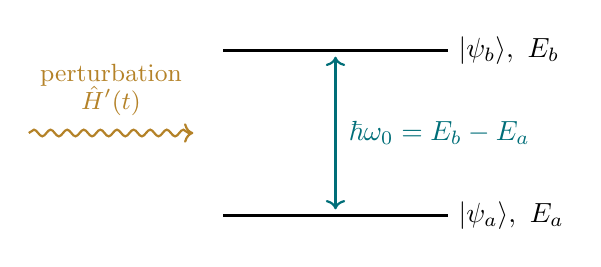
\begin{tikzpicture}[scale=0.95]
  \draw[line width=1.2pt] (0,0) -- (3,0) node[right] {$|\psi_a\rangle,\ E_a$};
  \draw[line width=1.2pt] (0,2.2) -- (3,2.2) node[right] {$|\psi_b\rangle,\ E_b$};
  \draw[<->,secondary,thick] (1.5,0.08) -- (1.5,2.12);
  \node[secondary,right] at (1.55,1.1) {$\hbar\omega_0 = E_b-E_a$};
  \draw[exframe,thick,decorate,decoration={snake,amplitude=1.2pt,segment length=6pt},->] (-2.6,1.1) -- (-0.4,1.1);
  \node[exframe,above,align=center] at (-1.5,1.2) {\small perturbation\\[-2pt]\small $\hat H'(t)$};
\end{tikzpicture}
\end{center}

At $t=0$ any state is a superposition $|\psi(0)\rangle = c_a|\psi_a\rangle + c_b|\psi_b\rangle$. Without the perturbation it would evolve as
\[
|\psi(t)\rangle = c_a\exp\Big(-\frac{iE_at}{\hbar}\Big)|\psi_a\rangle + c_b\exp\Big(-\frac{iE_bt}{\hbar}\Big)|\psi_b\rangle
\]
Here $|c_a|^2$ is the probability to find the particle in state $a$, similarly $|c_b|^2$ for state $b$, and $|c_a|^2+|c_b|^2=1$.

Now include $\hat H'(t)$. The coefficients become time-dependent:
\[
|\psi(t)\rangle = c_a(t)\exp\Big(-\frac{iE_at}{\hbar}\Big)|\psi_a\rangle + c_b(t)\exp\Big(-\frac{iE_bt}{\hbar}\Big)|\psi_b\rangle
\]
Insert into $(\hat H^0+\hat H'(t))|\psi(t)\rangle = i\hbar\,\partial_t|\psi(t)\rangle$. The $E_a$ and $E_b$ terms from $\hat H^0$ cancel against the same terms from the time derivative of the phase factors, leaving
\[
c_a e^{-iE_at/\hbar}\hat H'|\psi_a\rangle + c_b e^{-iE_bt/\hbar}\hat H'|\psi_b\rangle = i\hbar\,\dot c_a\, e^{-iE_at/\hbar}|\psi_a\rangle + i\hbar\,\dot c_b\, e^{-iE_bt/\hbar}|\psi_b\rangle
\]
Take the inner product with $\langle\psi_a|$ (using $\langle\psi_a|\psi_b\rangle=0$), and define $H'_{ij}=\langle\psi_i|\hat H'|\psi_j\rangle$:
\[
c_a e^{-iE_at/\hbar}H'_{aa} + c_b e^{-iE_bt/\hbar}H'_{ab} = i\hbar\,\dot c_a e^{-iE_at/\hbar}
\;\Longrightarrow\;
\dot c_a = -\frac{i}{\hbar}\Big[c_aH'_{aa} + c_bH'_{ab}\exp\Big(-\frac{i}{\hbar}(E_b-E_a)t\Big)\Big]
\]
Taking the inner product with $\langle\psi_b|$ instead gives
\[
\dot c_b = -\frac{i}{\hbar}\Big[c_bH'_{bb} + c_aH'_{ba}\exp\Big(\frac{i}{\hbar}(E_b-E_a)t\Big)\Big]
\]
Diagonal elements are taken as zero, $H'_{aa}=H'_{bb}=0$ (they only shift the energies and are absorbed into the levels).

\begin{thm}{Coupled Equations for the Two-Level System}
\[
\dot c_a(t) = -\frac{i}{\hbar}\,H'_{ab}\,e^{-i\omega_0t}\,c_b(t), \qquad
\dot c_b(t) = -\frac{i}{\hbar}\,H'_{ba}\,e^{i\omega_0t}\,c_a(t), \qquad \omega_0 = \frac{E_b-E_a}{\hbar}
\]
\end{thm}

\textbf{*** Study Note:} These equations are \textit{exact}; no approximation has been made yet. The approximation enters only when they are solved iteratively below. Hermiticity gives $H'_{ba}=(H'_{ab})^*$, and the exponentials $e^{\pm i\omega_0t}$ are the beating between the two levels: the coupling is effective only if $\hat H'(t)$ itself has a component oscillating near $\omega_0$.

\subsection{Perturbative Solution Order by Order}
Solve the coupled equations by iteration. Let $c^{(n)}$ denote the $n$-th iterate, i.e.\ the amplitude correct to order $\hat H'^{\,n}$. The initial condition fixes the zeroth iterate:
\[
c_a(0)=1,\qquad c_b(0)=0 \quad\Longrightarrow\quad c_a^{(0)}(t)=1,\quad c_b^{(0)}(t)=0
\]
Each iterate is obtained by inserting the previous iterate of the \textit{other} level into the right-hand side:
\[
\dot c_a^{(n)}(t) = -\frac{i}{\hbar}H'_{ab}e^{-i\omega_0t}c_b^{(n-1)}(t), \qquad
\dot c_b^{(n)}(t) = -\frac{i}{\hbar}H'_{ba}e^{i\omega_0t}c_a^{(n-1)}(t)
\]

\paragraph{First order.} $\dot c_a^{(1)} = -\frac i\hbar H'_{ab}e^{-i\omega_0t}c_b^{(0)}=0$, so $c_a^{(1)}$ is constant, and the initial condition $c_a(0)=1$ gives $c_a^{(1)}(t)=1$: there is no first-order correction to $c_a$. Then
\[
\dot c_b^{(1)}(t) = -\frac i\hbar H'_{ba}e^{i\omega_0t}c_a^{(0)} = -\frac i\hbar H'_{ba}e^{i\omega_0t}
\;\Longrightarrow\;
c_b^{(1)}(t) = -\frac i\hbar\int_0^t dt'\,H'_{ba}(t')\,e^{i\omega_0t'}
\]

\paragraph{Second order.} Now $c_b^{(1)}\neq0$ feeds back into $c_a$:
\[
\dot c_a^{(2)}(t) = -\frac i\hbar H'_{ab}e^{-i\omega_0t}\Big[-\frac i\hbar\int_0^tdt'\,H'_{ba}e^{i\omega_0t'}\Big]
\]
Integrating, with the constant of integration fixed by $c_a(0)=1$,
\[
c_a^{(2)}(t) = 1 - \frac1{\hbar^2}\int_0^tdt'\,H'_{ab}(t')e^{-i\omega_0t'}\int_0^{t'}dt''\,H'_{ba}(t'')e^{i\omega_0t''}
\]
For $c_b$, the driving term is $c_a^{(1)}=1$, exactly as in the first iterate, so $\dot c_b^{(2)}=\dot c_b^{(1)}$ and $c_b^{(2)}(t)=c_b^{(1)}(t)$: the first correction to $c_b$ beyond $\hat H'$ appears only at third order.

\begin{thm}{Two-Level Amplitudes to Second Order}
\begin{align*}
c_b^{(1)}(t) &= -\frac i\hbar\int_0^tdt'\,H'_{ba}(t')\,e^{i\omega_0t'} \qquad (c_b^{(2)}=c_b^{(1)})\\
c_a^{(2)}(t) &= 1-\frac1{\hbar^2}\int_0^tdt'\,H'_{ab}(t')\,e^{-i\omega_0t'}\int_0^{t'}dt''\,H'_{ba}(t'')\,e^{i\omega_0t''}
\end{align*}
\end{thm}

\textbf{*** Verification (probability conservation):} To order $\hat H'^2$,
\[
|c_a|^2 = 1-2\,\mathrm{Re}\,\frac1{\hbar^2}\int_0^tdt'\int_0^{t'}dt''\,H'_{ab}(t')H'_{ba}(t'')\,e^{-i\omega_0(t'-t'')}
\]
Adding the real parts of the double integral over the triangle $t''<t'$ and its mirror image gives the integral over the full square, which equals $\frac1{\hbar^2}\big|\int_0^tdt'\,H'_{ba}e^{i\omega_0t'}\big|^2=|c_b^{(1)}|^2$. Hence $|c_a|^2+|c_b|^2=1$ to second order.

\textbf{*** Study Note (notation):} The superscript counts iterations (amplitude correct to that order), so $c_a^{(1)}=1$; the notebook also writes ``$c_a^{(1)}=0$'' at one point, meaning that the first-order \textit{correction} to $c_a$ vanishes. Both statements are the same fact.

\textbf{*** Memory Rule:} Each factor of $\hat H'$ moves the system once between the levels; an even number of kicks brings it back to $a$, an odd number to $b$. That is why, starting from $a$, the corrections to $c_a$ come only at even orders and those to $c_b$ only at odd orders.

\subsection{Example: Sinusoidal Perturbation}
\begin{prob}{Example: Sinusoidal Perturbation $\hat H'(\vec r,t)=V(\vec r)\cos\omega t$}
Here $H'_{ab}=V_{ab}\cos\omega t$ and $H'_{ba}=V_{ba}\cos\omega t$. The first-order amplitude is
\begin{align*}
c_b(t) &= -\frac i\hbar\int_0^tdt'\,H'_{ba}e^{i\omega_0t'} = -\frac i\hbar V_{ba}\int_0^tdt'\,e^{i\omega_0t'}\cos\omega t'\\
&= -\frac{V_{ba}}{2\hbar}\left[\frac{e^{i(\omega_0+\omega)t}-1}{\omega_0+\omega} + \frac{e^{i(\omega_0-\omega)t}-1}{\omega_0-\omega}\right]
\end{align*}
\textbf{*** Complete Solution of the integral:} write $\cos\omega t'=\tfrac12(e^{i\omega t'}+e^{-i\omega t'})$, so $\int_0^t e^{i\omega_0t'}\cos\omega t'\,dt' = \tfrac12\Big[\frac{e^{i(\omega_0+\omega)t}-1}{i(\omega_0+\omega)}+\frac{e^{i(\omega_0-\omega)t}-1}{i(\omega_0-\omega)}\Big]$, and the factor $-\frac i\hbar\cdot\frac1{2i}=-\frac1{2\hbar}$ gives the result above.
\end{prob}

Let $\omega$ be the \textbf{driving frequency} and $\omega_0$ the \textbf{transition frequency}. If $\omega\approx\omega_0$, then $\omega+\omega_0\gg|\omega-\omega_0|$ and the first term (denominator $\omega_0+\omega$) is negligible compared with the second, which is large:
\begin{align*}
c_b(t) &\simeq -\frac{V_{ba}}{2\hbar}\,\frac{e^{i(\omega_0-\omega)t}-1}{\omega_0-\omega}
= -\frac{V_{ba}}{2\hbar}\,\frac{e^{\frac i2(\omega_0-\omega)t}}{\omega_0-\omega}\Big[e^{\frac i2(\omega_0-\omega)t}-e^{-\frac i2(\omega_0-\omega)t}\Big]\\
&= -\frac{iV_{ba}}{\hbar}\,\frac{\sin\!\big[\frac{\omega_0-\omega}2t\big]}{\omega_0-\omega}\,\exp\Big[\frac{i(\omega_0-\omega)t}2\Big]
\end{align*}
Hence the probability of a transition $a\to b$ is
\begin{thm}{Transition Probability for a Sinusoidal Perturbation}
\[
P_{a\to b}(t) = |c_b(t)|^2 \simeq \Big(\frac{|V_{ba}|}{\hbar}\Big)^2\frac{\sin^2\!\big[\frac{\omega_0-\omega}{2}\,t\big]}{(\omega_0-\omega)^2}
\]
\end{thm}

\begin{center}
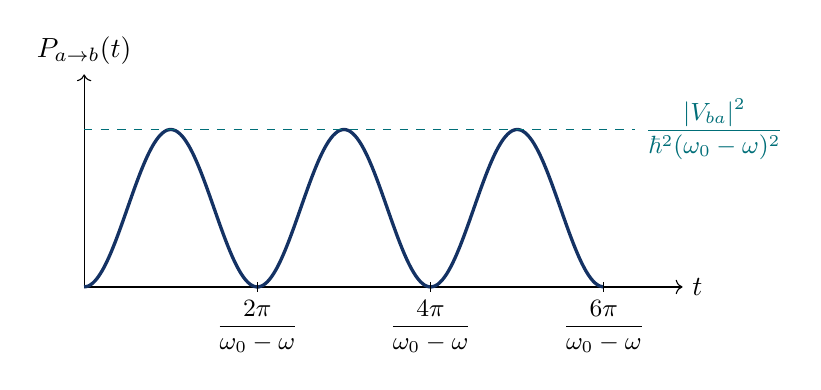
\begin{tikzpicture}[scale=1]
  \draw[->] (0,0) -- (7.6,0) node[right] {$t$};
  \draw[->] (0,0) -- (0,2.7) node[above] {$P_{a\to b}(t)$};
  \draw[very thick,primary,domain=0:6.6,samples=120,smooth] plot (\x,{2.0*(sin(\x*180/2.2))^2});
  \draw[dashed,secondary] (0,2.0) -- (7.0,2.0);
  \node[secondary,right] at (7.0,2.0) {\small $\dfrac{|V_{ba}|^2}{\hbar^2(\omega_0-\omega)^2}$};
  \foreach \x/\l in {2.2/{2\pi}, 4.4/{4\pi}, 6.6/{6\pi}} {
    \draw (\x,0.06) -- (\x,-0.06);
    \node[below] at (\x,-0.05) {\small $\dfrac{\l}{\omega_0-\omega}$};
  }
\end{tikzpicture}
\end{center}

\textbf{*** Study Note (sketch):} $P_{a\to b}(t)$ oscillates between $0$ and the fixed maximum $|V_{ba}|^2/\hbar^2(\omega_0-\omega)^2$ with zeros at $t=2\pi n/(\omega_0-\omega)$. The notebook sketch draws the successive arcs with decreasing height; for fixed $\omega$ the arcs all have the same height, as in the figure above.

\textbf{*** Study Note (rotating-wave approximation):} Dropping the term with denominator $\omega_0+\omega$ (the ``counter-rotating'' term) is the \textbf{rotating-wave approximation}. It is excellent near resonance and fails for $\omega$ far from $\omega_0$.

\textbf{*** Study Note (validity at resonance):} For $\omega\to\omega_0$, $\sin^2(\Delta t/2)/\Delta^2\to t^2/4$ (with $\Delta=\omega_0-\omega$), so $P_{a\to b}\to(|V_{ba}|t/2\hbar)^2$ grows quadratically and exceeds $1$ for $t\gtrsim2\hbar/|V_{ba}|$. First-order theory requires $P\ll1$, i.e.\ it breaks down on resonance for long times; the exact two-level solution (Section~\ref{td:sec:rabi}) replaces the quadratic growth by bounded oscillations.

\textbf{*** Exam Tip:} Always check the order of magnitude of the amplitude: transition probabilities from first-order theory are trustworthy only when $|V_{ba}|\ll\hbar|\omega_0-\omega|$ or the interaction time is short.
%==============================================================================
\section{The Interaction Picture}
%==============================================================================

\subsection{From the Schr\"odinger Picture to the Interaction Picture}
In the Schr\"odinger picture the states evolve in time with the full Hamiltonian. For a time-independent $\hat H$ the evolution operator is
\[
\hat U = \exp\Big(-\frac i\hbar\hat Ht\Big), \qquad |\psi(t)\rangle = \hat U|\psi(0)\rangle = \exp\Big(-\frac i\hbar\hat Ht\Big)|\psi(0)\rangle
\]
Expanding $|\psi(0)\rangle=\sum_n c_n(0)|n\rangle$ in the eigenstates, $\hat H|n\rangle=E_n|n\rangle$,
\[
|\psi(t)\rangle = \exp\Big(-\frac i\hbar\hat Ht\Big)\sum_nc_n|n\rangle = \sum_n\exp\Big(-\frac i\hbar E_nt\Big)c_n|n\rangle,
\qquad
i\hbar\frac\partial{\partial t}|\psi(t)\rangle_S = \hat H|\psi(t)\rangle_S
\]
The Schr\"odinger picture is not convenient for a time-dependent perturbation: the large, known evolution due to $\hat H^0$ is mixed with the small effect of $\hat V(t)$. We therefore switch to the \textbf{interaction picture}. With
\[
\hat H = \hat H^0 + \hat V(t)
\]
define the interaction-picture state
\[
|\psi(t)\rangle_I = \exp\Big(\frac i\hbar\hat H^0t\Big)|\psi(t)\rangle_S, \qquad\text{with}\quad |\psi(0)\rangle_I=|\psi(0)\rangle_S\ \text{at } t=0
\]
Differentiate and use the Schr\"odinger equation $i\hbar\,\partial_t|\psi\rangle_S=\hat H|\psi\rangle_S$:
\begin{align*}
i\hbar\frac\partial{\partial t}|\psi(t)\rangle_I &= i\hbar\Big[\frac{i\hat H^0}{\hbar}e^{\frac i\hbar\hat H^0t}|\psi(t)\rangle_S + e^{\frac i\hbar\hat H^0t}\,\partial_t|\psi(t)\rangle_S\Big]\\
&= -\hat H^0e^{\frac i\hbar\hat H^0t}|\psi(t)\rangle_S + e^{\frac i\hbar\hat H^0t}\hat H|\psi(t)\rangle_S
= e^{\frac i\hbar\hat H^0t}\big[\hat H-\hat H^0\big]|\psi(t)\rangle_S\\
&= e^{\frac i\hbar\hat H^0t}\,\hat V(t)\,|\psi(t)\rangle_S
= e^{\frac i\hbar\hat H^0t}\,\hat V(t)\,e^{-\frac i\hbar\hat H^0t}\,|\psi(t)\rangle_I
\end{align*}
\begin{thm}{Schr\"odinger Equation in the Interaction Picture}
\[
i\hbar\frac\partial{\partial t}|\psi(t)\rangle_I = \hat V_I(t)\,|\psi(t)\rangle_I, \qquad
\hat V_I(t) = \exp\Big(\frac i\hbar\hat H^0t\Big)\,\hat V(t)\,\exp\Big(-\frac i\hbar\hat H^0t\Big)
\]
\end{thm}
In the interaction picture \textbf{both operators and states have time dependence}.

\textbf{*** Intuition:} The factor $e^{\frac i\hbar\hat H^0t}$ ``undoes'' the fast, exactly known evolution of the unperturbed system. What is left evolves only because of the perturbation, and it is driven by $\hat V_I(t)$ alone, which is small. This is exactly why a power series in $\hat V$ makes sense.

\textbf{*** Memory Rule:} Operators evolve with $\hat H^0$ (that is the factor $e^{\pm i\hat H^0t/\hbar}$ in $\hat V_I$); states evolve only under $\hat V_I$. If $\hat V=0$ the interaction-picture state is constant.

\textbf{*** Study Note:} The two pictures give the same physics: the probability $|c_n|^2$ of finding the system in the eigenstate $|n\rangle$ of $\hat H^0$ is identical in both, because $e^{\frac i\hbar\hat H^0t}$ is unitary and only multiplies each $|n\rangle$ by a phase $e^{iE_nt/\hbar}$.

\subsection{Equation for the Coefficients}
Expand the interaction-picture state in the eigenstates of $\hat H^0$ (with $\hat H^0|n\rangle=E_n|n\rangle$):
\[
|\psi(t)\rangle_I = \sum_nc_n(t)|n\rangle
\]
Insert in $i\hbar\,\partial_t|\psi\rangle_I=\hat V_I|\psi\rangle_I$:
\[
i\hbar\sum_n\dot c_n(t)|n\rangle = \exp\Big(\frac i\hbar\hat H^0t\Big)\hat V(t)\exp\Big(-\frac i\hbar\hat H^0t\Big)\sum_nc_n(t)|n\rangle
\]
Take the inner product with $\langle m|$ and use $\langle m|e^{\frac i\hbar\hat H^0t}=e^{\frac i\hbar E_mt}\langle m|$:
\[
i\hbar\,\dot c_m(t) = \sum_n\exp\Big(\frac i\hbar(E_m-E_n)t\Big)\langle m|\hat V(t)|n\rangle\,c_n(t)
\]
Define the matrix element and the transition frequency
\[
V_{mn}(t)=\langle m|\hat V(t)|n\rangle, \qquad \hbar\omega_{mn}=E_m-E_n, \qquad \omega_{nm}=-\omega_{mn}
\]
\begin{thm}{Coupled Equations for the Amplitudes in the Interaction Picture}
\[
i\hbar\,\dot c_m(t) = \sum_nV_{mn}(t)\,e^{i\omega_{mn}t}\,c_n(t)
\]
\end{thm}

\textbf{*** Study Note (consistency with Section 1):} For two levels $a,b$ with $\omega_{ba}=\omega_0$ this gives $\dot c_b=-\frac i\hbar V_{ba}e^{i\omega_0t}c_a$ and $\dot c_a=-\frac i\hbar V_{ab}e^{-i\omega_0t}c_b$, the same equations that were derived directly in Section~\ref{td:sec:two}.

\textbf{*** Exam Tip:} This set of equations is the starting point for \textit{every} problem in this chapter: truncate the sum to the relevant levels and solve (exactly for two levels, iteratively in general).
%==============================================================================
\section{Two-Level System with an Oscillating Coupling: Exact Solution}
\label{td:sec:rabi}
%==============================================================================

\subsection{The Model}
Consider two levels $|1\rangle,|2\rangle$ with energies $E_1<E_2$ and a perturbation that couples them with an oscillating amplitude:
\begin{align*}
\hat H^0 &= E_1|1\rangle\langle1| + E_2|2\rangle\langle2| = \begin{pmatrix}E_1&0\\0&E_2\end{pmatrix}\\
\hat V(t) &= \delta\,e^{i\omega t}|1\rangle\langle2| + \delta\,e^{-i\omega t}|2\rangle\langle1| = \begin{pmatrix}0&\delta\,e^{i\omega t}\\ \delta\,e^{-i\omega t}&0\end{pmatrix}
\end{align*}
so that $\hat H^0+\hat V(t)=\begin{pmatrix}E_1&\delta e^{i\omega t}\\ \delta e^{-i\omega t}&E_2\end{pmatrix}$. If diagonal terms were present in $\hat V$ they would just shift $E_1,E_2$ and are neglected.

\begin{center}
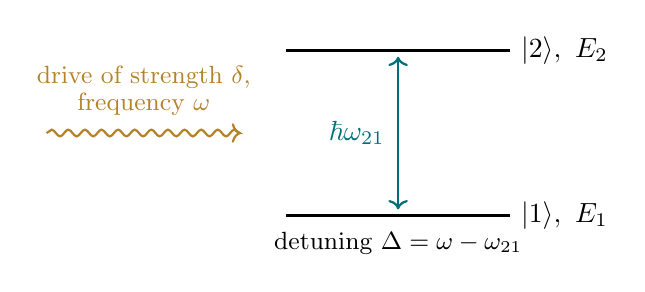
\begin{tikzpicture}[scale=0.95]
  \draw[line width=1.2pt] (0,0) -- (3,0) node[right] {$|1\rangle,\ E_1$};
  \draw[line width=1.2pt] (0,2.2) -- (3,2.2) node[right] {$|2\rangle,\ E_2$};
  \draw[<->,secondary,thick] (1.5,0.08) -- (1.5,2.12);
  \node[secondary,left] at (1.45,1.1) {$\hbar\omega_{21}$};
  \draw[exframe,thick,decorate,decoration={snake,amplitude=1.2pt,segment length=6pt},->] (-3.2,1.1) -- (-0.6,1.1);
  \node[exframe,above,align=center] at (-1.9,1.2) {\small drive of strength $\delta$,\\[-2pt]\small frequency $\omega$};
  \node[below] at (1.5,-0.1) {\small detuning $\Delta=\omega-\omega_{21}$};
\end{tikzpicture}
\end{center}

\textbf{*** Study Note:} $\hat V$ is Hermitian because $V_{21}=V_{12}^*$. The model is the standard picture of a two-level atom driven by a field of frequency $\omega$ in the rotating-wave approximation, with $\delta$ the coupling strength and $\Delta=\omega-\omega_{21}$ the detuning from resonance.

\subsection{Equations of Motion and Their Solution}
Use the interaction-picture equation $i\hbar\dot c_m=\sum_nV_{mn}e^{i\omega_{mn}t}c_n$ with $V_{11}=V_{22}=0$, $V_{12}=\delta e^{i\omega t}$, $V_{21}=\delta e^{-i\omega t}$ and $\omega_{12}=-\omega_{21}$:
\[
i\hbar\,\dot c_1(t) = V_{12}e^{i\omega_{12}t}c_2 = \delta\,e^{i\omega t}e^{-i\omega_{21}t}c_2 = \delta\,e^{i(\omega-\omega_{21})t}c_2(t)
\]
In matrix form,
\[
i\hbar\begin{pmatrix}\dot c_1(t)\\ \dot c_2(t)\end{pmatrix}
= \delta\begin{pmatrix}0&e^{i(\omega-\omega_{21})t}\\ e^{-i(\omega-\omega_{21})t}&0\end{pmatrix}\begin{pmatrix}c_1(t)\\ c_2(t)\end{pmatrix}
\]
\begin{thm}{Equations of Motion of the Driven Two-Level System}
\begin{align*}
i\hbar\,\dot c_1(t) &= \delta\,\exp\big[i(\omega-\omega_{21})t\big]\,c_2(t)\\
i\hbar\,\dot c_2(t) &= \delta\,\exp\big[-i(\omega-\omega_{21})t\big]\,c_1(t)
\end{align*}
Initial condition: $c_1(0)=1,\ c_2(0)=0$.
\end{thm}

Write $\Delta=\omega-\omega_{21}$ for the detuning. Differentiate the second equation:
\begin{align*}
i\hbar\,\ddot c_2 &= -i\Delta\,\delta e^{-i\Delta t}c_1 + \delta e^{-i\Delta t}\dot c_1
= -i\Delta\,(i\hbar\dot c_2) + \delta e^{-i\Delta t}\cdot\frac{\delta e^{i\Delta t}c_2}{i\hbar}
\end{align*}
and dividing by $i\hbar$ gives the second-order equation
\[
\ddot c_2(t) + i\Delta\,\dot c_2(t) + \Big(\frac\delta\hbar\Big)^2c_2(t)=0
\]

\textbf{*** Complete Solution:} Put $c_2(t)=e^{-i\Delta t/2}f(t)$. Then $\dot c_2=e^{-i\Delta t/2}(\dot f-\tfrac{i\Delta}2f)$, $\ddot c_2=e^{-i\Delta t/2}(\ddot f-i\Delta\dot f-\tfrac{\Delta^2}4f)$, and substituting,
\[
\ddot f + \Big[\frac{\Delta^2}{4}+\Big(\frac\delta\hbar\Big)^2\Big]f = \ddot f+\Omega^2f=0, \qquad
\Omega=\Big[\Big(\frac\delta\hbar\Big)^2+\frac{(\omega-\omega_{21})^2}4\Big]^{1/2}
\]
The conditions $c_2(0)=0\Rightarrow f(0)=0$ and $\dot c_2(0)=-\frac{i\delta}{\hbar}c_1(0)=-\frac{i\delta}\hbar$ (from the equation of motion) fix $f=-\dfrac{i\delta}{\hbar\Omega}\sin\Omega t$. Hence
\begin{thm}{Rabi Oscillations}
\[
c_2(t) = -\frac{i\delta}{\hbar\Omega}\,\exp\Big[-i(\omega-\omega_{21})\frac t2\Big]\sin\Omega t, \qquad
\Omega=\Big[\Big(\frac\delta\hbar\Big)^2+\frac{(\omega-\omega_{21})^2}4\Big]^{1/2}\ \ (\text{Rabi frequency})
\]
\[
P_{1\to2}(t)=|c_2(t)|^2 = \Big(\frac{\delta}{\hbar\Omega}\Big)^2\sin^2\Omega t
= \frac{(\delta/\hbar)^2}{(\delta/\hbar)^2+(\omega-\omega_{21})^2/4}\,\sin^2\Omega t
\]
\end{thm}

\textbf{*** Study Note (correction):} The notebook writes $c_2(t)=\exp[-i(\omega-\omega_{21})t/2]\sin\Omega t$ and $|c_2|^2=\sin^2\Omega t$, omitting the amplitude factor $-i\delta/\hbar\Omega$. The factor is required by $\dot c_2(0)=-i\delta/\hbar$ and by normalization, and it equals $1$ only on resonance ($\omega=\omega_{21}$). Without it $|c_2|^2$ would reach $1$ for any detuning, which is false.

\textbf{*** Complete Solution (the other amplitude):} From $i\hbar\dot c_2=\delta e^{-i\Delta t}c_1$,
\[
c_1(t)=e^{i\Delta t/2}\Big[\cos\Omega t-\frac{i\Delta}{2\Omega}\sin\Omega t\Big]
\]
\textbf{*** Verification:} $|c_1|^2+|c_2|^2=\cos^2\Omega t+\dfrac{\Delta^2/4+(\delta/\hbar)^2}{\Omega^2}\sin^2\Omega t=1$ \checkmark. For $\delta\to0$, $\Omega\to|\Delta|/2$ and $P_{1\to2}\to\dfrac{4\delta^2}{\hbar^2\Delta^2}\sin^2\dfrac{\Delta t}2$, which is the first-order result of Section~\ref{td:sec:two} (a drive $V_{ba}\cos\omega t$ corresponds to $\delta=V_{ba}/2$ in the rotating-wave approximation).

\begin{center}
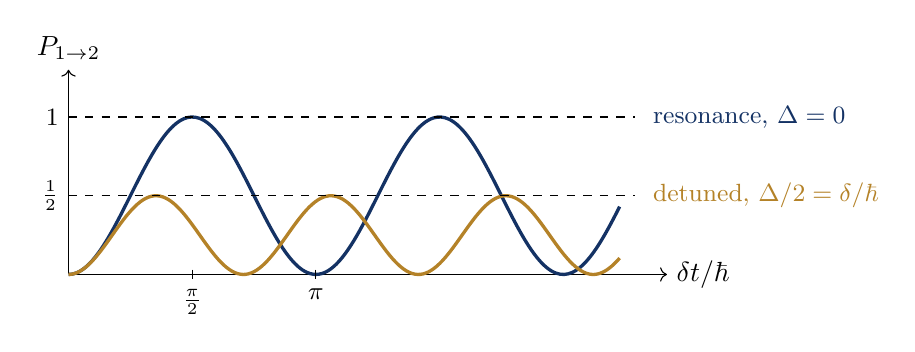
\begin{tikzpicture}[scale=1]
  \draw[->] (0,0) -- (7.6,0) node[right] {$\delta t/\hbar$};
  \draw[->] (0,0) -- (0,2.6) node[above] {$P_{1\to2}$};
  \draw[very thick,primary,domain=0:7,samples=140,smooth] plot (\x,{2.0*(sin(\x*57.2958))^2});
  \draw[very thick,exframe,domain=0:7,samples=200,smooth] plot (\x,{2.0*0.5*(sin(1.4142*\x*57.2958))^2});
  \draw[dashed] (0,2.0) -- (7.2,2.0); \node[left] at (0,2.0) {\small $1$};
  \draw[dashed] (0,1.0) -- (7.2,1.0); \node[left] at (0,1.0) {\small $\tfrac12$};
  \node[primary,right] at (7.3,2.0) {\small resonance, $\Delta=0$};
  \node[exframe,right] at (7.3,1.0) {\small detuned, $\Delta/2=\delta/\hbar$};
  \draw (1.5708,0.06) -- (1.5708,-0.06) node[below] {\small $\frac\pi2$};
  \draw (3.1416,0.06) -- (3.1416,-0.06) node[below] {\small $\pi$};
\end{tikzpicture}
\end{center}
\textbf{*** Study Note (figure):} On resonance the system is completely transferred $1\to2$ at $t=\pi\hbar/2\delta$ (a ``$\pi$-pulse'') and back at $t=\pi\hbar/\delta$. Off resonance the maximum transfer is only $(\delta/\hbar\Omega)^2<1$ and the oscillation is faster (the plot uses $\Delta/2=\delta/\hbar$, giving $\Omega=\sqrt2\,\delta/\hbar$ and maximum $\tfrac12$). The probability oscillates at angular frequency $2\Omega$.

\textbf{*** Exam Tip:} Three things to remember: (i) the Rabi frequency $\Omega=\sqrt{(\delta/\hbar)^2+\Delta^2/4}$, (ii) the maximum transfer $(\delta/\hbar\Omega)^2$ (a Lorentzian in the detuning, equal to $1$ at resonance), (iii) $P(t)=(\delta/\hbar\Omega)^2\sin^2\Omega t$ is exact; first-order theory is its small-$\delta$ limit.
%==============================================================================
\section{The Dyson Series and General Transition Amplitudes}
%==============================================================================

\subsection{The Time-Evolution Operator in the Interaction Picture}
Define the evolution operator by
\[
|\psi(t)\rangle_I = \hat U_I(t,t_0)\,|\psi(t_0)\rangle_I
\]
Substituting in $i\hbar\,\partial_t|\psi(t)\rangle_I=\hat V_I(t)|\psi(t)\rangle_I$ gives the equation for the operator itself:
\[
i\hbar\frac\partial{\partial t}\hat U_I(t,t_0)=\hat V_I(t)\,\hat U_I(t,t_0)
\;\Longrightarrow\;
\int_{t_0}^t\partial\hat U_I(t',t_0)=-\frac i\hbar\int_{t_0}^t\hat V_I(t')\hat U_I(t',t_0)\,dt'
\]
Since $\hat U_I(t_0,t_0)=\mathbb 1$, this is the integral equation
\[
\hat U_I(t,t_0) = \mathbb 1 - \frac i\hbar\int_{t_0}^tdt'\,\hat V_I(t')\,\hat U_I(t',t_0)
\]
Insert the right-hand side into itself repeatedly (iteration):
\begin{align*}
\hat U_I(t,t_0) &= \mathbb 1 - \frac i\hbar\int_{t_0}^tdt'\,\hat V_I(t')\Big[\mathbb 1-\frac i\hbar\int_{t_0}^{t'}dt''\,\hat V_I(t'')\hat U_I(t'',t_0)\Big]\\
&= \mathbb 1 - \frac i\hbar\int_{t_0}^tdt'\,\hat V_I(t') + \Big(-\frac i\hbar\Big)^2\int_{t_0}^tdt'\int_{t_0}^{t'}dt''\,\hat V_I(t')\hat V_I(t'')\hat U_I(t'',t_0)
\end{align*}
and so on. This is the \textbf{Dyson series}:
\begin{thm}{Dyson Series}
\[
\hat U_I(t,t_0) = \sum_{n=0}^\infty\Big(-\frac i\hbar\Big)^n\int_{t_0}^tdt_1\int_{t_0}^{t_1}dt_2\cdots\int_{t_0}^{t_{n-1}}dt_n\;\hat V_I(t_1)\hat V_I(t_2)\cdots\hat V_I(t_n)
\]
with the time ordering $t_0<t_n<t_{n-1}<\cdots<t_2<t_1<t$. The remainder is negligible because it contains high powers of $\hat V$.
\end{thm}
The same series is written with a \textbf{time-ordered product} $T$, which places operators at later times to the left, $\hat U_I=\sum_n(-\frac i\hbar)^nT\int_{t_0}^t dt_1\cdots dt_n\,\hat V_I(t_1)\cdots\hat V_I(t_n)$, where each ``time slice'' obeys the ordering above.

\begin{center}
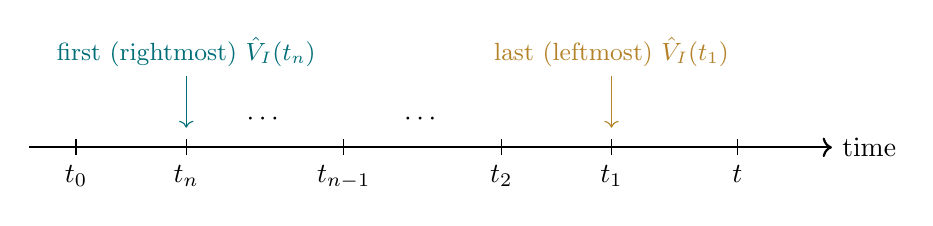
\begin{tikzpicture}[scale=1]
  \draw[->,thick] (0,0) -- (10.2,0) node[right] {time};
  \foreach \x/\l in {0.6/t_0, 2.0/t_n, 4.0/t_{n-1}, 6.0/t_2, 7.4/t_1, 9.0/t} {
    \draw (\x,0.1) -- (\x,-0.1); \node[below] at (\x,-0.1) {$\l$};
  }
  \node at (3.0,0.35) {$\cdots$}; \node at (5.0,0.35) {$\cdots$};
  \draw[<-,secondary] (2.0,0.25) -- (2.0,0.9) node[above] {\small first (rightmost) $\hat V_I(t_n)$};
  \draw[<-,exframe] (7.4,0.25) -- (7.4,0.9) node[above] {\small last (leftmost) $\hat V_I(t_1)$};
\end{tikzpicture}
\end{center}

\textbf{*** Intuition:} The $n$-th term is the sum over all histories in which the system receives $n$ kicks of $\hat V_I$ at ordered times. Earlier kicks act first, so they stand to the \textit{right} of later ones.

\textbf{*** Memory Rule:} Latest time on the left; nested limits $t_0<t_n<\cdots<t_1<t$ guarantee that each ordering of the same $n$ times is counted exactly once.

\subsection{Transition Amplitudes}
If the system is prepared in an initial eigenstate $|i\rangle$ of $\hat H^0$ at $t=t_0$, then at a later time it is in the final state
\[
|f\rangle = \hat U_I(t,t_0)|i(t_0)\rangle = \sum_n|n\rangle\langle n|\hat U_I(t,t_0)|i(t_0)\rangle=\sum_nc_n(t)|n\rangle,
\qquad c_n(t)=\langle n|\hat U_I(t,t_0)|i\rangle
\]
where $|n\rangle$ are the eigenstates of $\hat H^0$, $\hat H^0|n\rangle=E_n|n\rangle$. Expanding $\hat U_I$ with the Dyson series, $c_n(t)=c_n^{(0)}+c_n^{(1)}+c_n^{(2)}+\cdots$, with
\begin{align*}
c_n^{(0)}(t) &= \langle n|\mathbb 1|i\rangle = \delta_{ni}\\
c_n^{(1)}(t) &= -\frac i\hbar\int_{t_0}^tdt'\sum_m\langle n|\hat V_I(t')|m\rangle\langle m|i\rangle
\end{align*}
The matrix elements in the interaction picture are
\[
\langle n|\hat V_I(t)|m\rangle = e^{\frac i\hbar(E_n-E_m)t}\langle n|\hat V(t)|m\rangle = V_{nm}(t)\,e^{i\omega_{nm}t}
\]
so with $\langle m|i\rangle=\delta_{mi}$,
\[
c_n^{(1)}(t) = -\frac i\hbar\int_{t_0}^tdt'\,V_{ni}(t')\,e^{i\omega_{ni}t'}
\]
At second order,
\begin{align*}
c_n^{(2)}(t) &= \Big(-\frac i\hbar\Big)^2\int_{t_0}^tdt'\int_{t_0}^{t'}dt''\sum_{m,p}\langle n|\hat V_I(t')|m\rangle\langle m|\hat V_I(t'')|p\rangle\langle p|i\rangle\\
&= \Big(-\frac i\hbar\Big)^2\sum_m\int_{t_0}^tdt'\int_{t_0}^{t'}dt''\,V_{nm}(t')V_{mi}(t'')\,e^{i\omega_{nm}t'}e^{i\omega_{mi}t''}
\end{align*}
\begin{thm}{Transition Amplitudes and Probability}
\begin{align*}
c_n^{(1)}(t) &= -\frac i\hbar\int_{t_0}^tdt'\,V_{ni}(t')\,e^{i\omega_{ni}t'} \qquad\text{(first order formula)}\\
c_n^{(2)}(t) &= \Big(-\frac i\hbar\Big)^2\sum_m\int_{t_0}^tdt'\int_{t_0}^{t'}dt''\,V_{nm}(t')V_{mi}(t'')\,e^{i\omega_{nm}t'}e^{i\omega_{mi}t''} \qquad\text{(second order formula)}\\
P_{i\to n}(t) &= \Big|c_n^{(0)}(t)+c_n^{(1)}(t)+c_n^{(2)}(t)+\cdots\Big|^2 \qquad\text{(transition probability)}
\end{align*}
\end{thm}

\textbf{*** Study Note:} For two levels the first-order formula reduces to $c_b^{(1)}=-\frac i\hbar\int_0^tH'_{ba}e^{i\omega_0t'}dt'$ of Section~\ref{td:sec:two}. In the second-order formula the sum over $m$ runs over \textit{all} intermediate states (including $m=i$ and $m=n$); the intermediate state is ``virtual'': energy need not be conserved in the intermediate step.

\textbf{*** Memory Rule:} First order is the Fourier transform of the matrix element $V_{ni}(t)$ evaluated at the transition frequency $\omega_{ni}$. Second order is two such steps $i\to m\to n$, with the later step integrated over the shorter nested time.

\textbf{*** Exam Tip:} For $n\neq i$ the zeroth-order term vanishes and the leading probability is $|c_n^{(1)}|^2$. For $n=i$ (survival) $c_i\approx1$ and one uses $1-\sum_{n\neq i}P_{i\to n}$ instead.

\subsection{Example: Kicked Oscillator}
\begin{prob}{Example: Kicked Harmonic Oscillator}
\[
\hat H^0=\hbar\omega\Big(\hat a^\dagger\hat a+\tfrac12\Big)
\]
Initially ($t=-\infty$) the oscillator is in its ground state $|0\rangle$. It is perturbed by a weak transient electric field,
\[
\hat V(t) = -e\mathcal E\,\hat x\,\exp\Big(-\frac{t^2}{\tau^2}\Big)
\]
What is the probability of finding the particle in the first excited state $|1\rangle$ at $t=\infty$?

\medskip
\textbf{Solution.} $P_{0\to1}=|c_1^{(1)}|^2$ with
\[
c_1(t) = -\frac i\hbar\int_{-\infty}^{\infty}dt'\Big\{-e\mathcal E\exp\Big(-\frac{t'^2}{\tau^2}\Big)\Big\}\langle1|\hat x|0\rangle\,e^{i\omega_{10}t'},
\qquad
\langle1|\hat x|0\rangle=\sqrt{\frac\hbar{2m\omega}}\,\langle1|\hat a+\hat a^\dagger|0\rangle=\sqrt{\frac\hbar{2m\omega}}
\]
and $\omega_{10}=\omega$. The time integral is Gaussian:
\[
\int_{-\infty}^{\infty}e^{i\omega t'}e^{-t'^2/\tau^2}dt' = \sqrt\pi\,\tau\,\exp\Big(-\tfrac14\omega^2\tau^2\Big)
\]
so
\[
c_1(\infty) = +\frac i\hbar\sqrt{\frac\hbar{2m\omega}}\,e\mathcal E\sqrt\pi\,\tau\,\exp\Big(-\tfrac14\omega^2\tau^2\Big)
\]
\end{prob}
\begin{prob}{Example: Kicked Harmonic Oscillator (completed)}
\textbf{*** Complete Solution (Gaussian integral):} complete the square, $-\dfrac{t'^2}{\tau^2}+i\omega t'=-\Big(\dfrac{t'}\tau-\dfrac{i\omega\tau}2\Big)^2-\dfrac{\omega^2\tau^2}4$; the remaining integral $\int e^{-s^2/\tau^2}ds=\sqrt\pi\,\tau$ gives the result above.

\textbf{*** Complete Solution (probability):}
\[
\boxed{P_{0\to1}=|c_1|^2=\frac{\pi e^2\mathcal E^2\tau^2}{2m\hbar\omega}\exp\Big(-\frac{\omega^2\tau^2}2\Big)}
\]
\textbf{*** Verification and limits:} the combination $e^2\mathcal E^2/(m\hbar\omega^3)$ is dimensionless, as it must be (so $\omega\tau$ is the only other variable). For a very short pulse ($\omega\tau\ll1$) $P\propto\tau^2\to0$: the pulse area is small. For a very slow pulse ($\omega\tau\gg1$) the exponential makes $P$ extremely small: the oscillator follows adiabatically and returns to the ground state. The probability is largest for $\tau^2=2/\omega^2$, where $P_{\max}=\dfrac{\pi e^2\mathcal E^2}{m\hbar\omega^3}\exp(-1)$.
\end{prob}

\textbf{*** Study Note:} At first order only $|0\rangle\to|1\rangle$ is possible, because $\langle n|\hat x|0\rangle=0$ for $n\ge2$. The state $|2\rangle$ is reached at second order via the virtual intermediate state $|1\rangle$. The result is valid only if $P_{0\to1}\ll1$, i.e.\ for a weak field.

\begin{center}
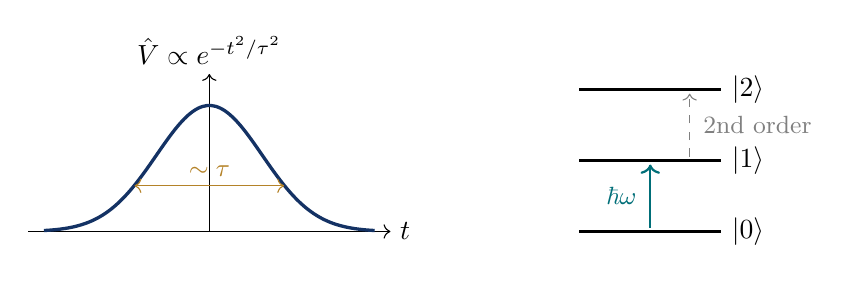
\begin{tikzpicture}[scale=1]
  \draw[->] (0,0) -- (4.6,0) node[right] {$t$};
  \draw[->] (2.3,0) -- (2.3,2.0) node[above] {$\hat V\propto e^{-t^2/\tau^2}$};
  \draw[very thick,primary,domain=-2.1:2.1,samples=80,smooth] plot ({2.3+\x},{1.6*exp(-\x*\x/0.9)});
  \draw[<->,exframe] (2.3-0.95,0.58) -- (2.3+0.95,0.58); \node[exframe,above] at (2.3,0.58) {\small $\sim\tau$};
  \foreach \y/\l in {0/{|0\rangle}, 0.9/{|1\rangle}, 1.8/{|2\rangle}} {
    \draw[line width=1.1pt] (7.0,\y) -- (8.8,\y) node[right] {$\l$};
  }
  \draw[->,secondary,thick] (7.9,0.05) -- (7.9,0.85); \node[secondary,left] at (7.85,0.45) {\small $\hbar\omega$};
  \draw[->,dashed,gray] (8.4,0.95) -- (8.4,1.75); \node[gray,right] at (8.45,1.35) {\small 2nd order};
\end{tikzpicture}
\end{center}
%==============================================================================
\section{Harmonic Perturbation and Fermi's Golden Rule}
\label{td:sec:fermi}
%==============================================================================

\subsection{Transition Probability for a Harmonic Perturbation}
The system starts in the initial state $|i\rangle$ and is perturbed by a periodic potential
\[
\hat V(t)=\hat v\,e^{-i\omega t}
\]
where $\hat v$ may depend on space but not on time. What is the probability that at a later time $t$ the system is in the final state $|f\rangle$? Use the first-order formula with $t_0=0$:
\[
c_f^{i\to f}(t) = -\frac i\hbar\int_0^tdt'\,\langle f|\hat v|i\rangle\,e^{i(\omega_{fi}-\omega)t'}
= -\frac i\hbar\langle f|\hat v|i\rangle\,\frac{e^{i(\omega_{fi}-\omega)t}-1}{i(\omega_{fi}-\omega)}
\]
Factor out the phase, $e^{i\Delta t}-1=e^{i\Delta t/2}\big(e^{i\Delta t/2}-e^{-i\Delta t/2}\big)=2i\,e^{i\Delta t/2}\sin(\Delta t/2)$ with $\Delta=\omega_{fi}-\omega$:
\[
c_f^{i\to f}(t) = -\frac i\hbar\langle f|\hat v|i\rangle\,\exp\Big[\frac i2(\omega_{fi}-\omega)t\Big]\,
\frac{\sin\!\big[\frac{(\omega_{fi}-\omega)t}2\big]}{(\omega_{fi}-\omega)/2}
\]
\begin{thm}{Transition Probability for $\hat V(t)=\hat v\,e^{-i\omega t}$}
\[
P_{i\to f}(t) = |c_f^{i\to f}|^2 = \frac1{\hbar^2}\,|\langle f|\hat v|i\rangle|^2\,
\frac{\sin^2\!\big[\frac{(\omega_{fi}-\omega)t}2\big]}{\big[\frac{\omega_{fi}-\omega}2\big]^2}
\]
\end{thm}
Put $\alpha=(\omega_{fi}-\omega)/2$, so that $P_{i\to f}=\frac1{\hbar^2}|\langle f|\hat v|i\rangle|^2\,\dfrac{\sin^2\alpha t}{\alpha^2}$. As a function of $\alpha$ this is a sharp peak at $\alpha=0$ of height $t^2$ and width of order $\pi/t$, with small side lobes:

\begin{center}
\begin{tikzpicture}[scale=1]
  \draw[->] (-5.2,0) -- (5.4,0) node[right] {$\alpha$};
  \draw[->] (0,0) -- (0,2.7) node[above] {$\sin^2\alpha t/\alpha^2$};
  \draw[very thick,primary,domain=-9.42:9.42,samples=300,smooth] plot ({\x*0.5},{2.4*ifthenelse(abs(\x)<0.01,1,(sin(deg(\x))/\x)^2)});
  \node[below] at (0.5*3.1416,-0.05) {\small $\pi/t$};
  \node[below] at (-0.5*3.1416,-0.05) {\small $-\pi/t$};
  \node[right] at (0.05,2.45) {\small $t^2$};
\end{tikzpicture}
\end{center}

\textbf{*** Intuition:} A harmonic perturbation only drives transitions whose frequency $\omega_{fi}$ matches the drive frequency $\omega$ to within about $1/t$: the longer the interaction, the sharper the resonance (an energy-time uncertainty relation, $\Delta E\,t\sim\hbar$).

\subsection{Fermi's Golden Rule}
The area under the peak is $\int_{-\infty}^\infty\frac{\sin^2\alpha t}{\alpha^2}d\alpha=\pi t$, proportional to $t$, while the peak narrows as $t$ grows. Hence for large $t$
\[
\lim_{t\to\infty}\frac1t\Big(\frac{\sin\alpha t}{\alpha}\Big)^2=\pi\,\delta(\alpha)
\]
Then
\[
\frac{P_{i\to f}}{t}=\frac1{\hbar^2}|\langle f|\hat v|i\rangle|^2\,\frac{\sin^2\alpha t}{t\,\alpha^2}
\;\xrightarrow{\,t\to\infty\,}\;\frac1{\hbar^2}|\langle f|\hat v|i\rangle|^2\,\pi\,\delta\Big(\frac{\omega_{fi}-\omega}2\Big)
\]
Using $\delta(x/2)=2\delta(x)$, this defines a constant transition rate $R^{i\to f}$ (probability per unit time):
\begin{thm}{Fermi's Golden Rule}
\[
R^{i\to f}=\frac{2\pi}{\hbar^2}\,|\langle f|\hat v|i\rangle|^2\,\delta(\omega_{fi}-\omega)
=\frac{2\pi}\hbar\,|\langle f|\hat v|i\rangle|^2\,\delta(E_f-E_i-\hbar\omega)
\]
\end{thm}
The second form follows from $\delta(\omega_{fi}-\omega)=\hbar\,\delta(E_f-E_i-\hbar\omega)$ (this is another statement of Fermi's golden rule).

If $\omega=0$ the perturbation is constant, and $\delta(\omega_{fi})=\delta(\omega_f-\omega_i)$ allows only $E_f=E_i$: a constant perturbation causes no real transition between states of different energy. The particle stays in the same (stationary) state.

\textbf{*** Study Note (validity):} The rate is linear in time only if the interaction is long enough that the peak is narrow compared with the spacing of the levels and that the energy distribution of the final states is smooth, i.e.\ $1/t\ll$ (spread of final energies$/\hbar$); but short enough that $P\ll1$. For a single discrete final level there is no $\delta$-function: the probability oscillates as in Section~\ref{td:sec:two} instead of growing linearly.

\textbf{*** Memory Rule:} Golden rule in words: rate $=\dfrac{2\pi}\hbar\times|\text{matrix element}|^2\times$ (density of final states at the energy-conserving final energy).

\subsection{Transition into a Continuum of Final States}
For a continuum define the \textbf{density of final states} $\rho(E_f)$: $\rho(E_f)\,dE_f$ is the number of final states with energy between $E_f$ and $E_f+dE_f$. The total transition rate to the continuum is
\begin{align*}
W_{if}&=\int\frac{P_{i\to f}(t)}t\,\rho(E_f)\,dE_f
=\frac{2\pi}\hbar\int dE_f\,|\langle f|\hat v|i\rangle|^2\,\delta(E_f-E_i-\hbar\omega)\,\rho(E_f)
\end{align*}
The delta function removes the integral:
\begin{thm}{Golden Rule for a Continuum}
\[
W_{if}=\frac{2\pi}\hbar\,|\langle f|\hat v|i\rangle|^2\,\rho(E_i+\hbar\omega)
\]
\end{thm}
\textbf{*** Exam Tip:} Whenever the final states form a continuum (ionization, decay into free particles, emission of a photon), use $W=\frac{2\pi}\hbar|\langle f|V|i\rangle|^2\rho$. The matrix element and $\rho$ must both be evaluated at the energy-conserving final energy.

\subsection{Harmonic Perturbation with Two Terms: Absorption and Stimulated Emission}
A real (Hermitian) oscillating perturbation contains both frequency signs:
\[
\hat V(t)=\hat v\,e^{i\omega t}+\hat v^\dagger e^{-i\omega t}
\]
The first-order probability is
\[
P_{i\to f}=\frac1{\hbar^2}\Big|\langle f|\hat v|i\rangle\int_0^tdt'\,e^{i(\omega_{fi}+\omega)t'}+\langle f|\hat v^\dagger|i\rangle\int_0^tdt'\,e^{i(\omega_{fi}-\omega)t'}\Big|^2
\]
The two terms peak at different frequencies ($\omega_{fi}=-\omega$ and $\omega_{fi}=+\omega$), so the cross terms are negligible:
\[
P_{i\to f}\simeq\frac4{\hbar^2}|\langle f|\hat v|i\rangle|^2\frac{\sin^2(\omega_{fi}+\omega)\frac t2}{(\omega_{fi}+\omega)^2}
+\frac4{\hbar^2}|\langle f|\hat v^\dagger|i\rangle|^2\frac{\sin^2(\omega_{fi}-\omega)\frac t2}{(\omega_{fi}-\omega)^2}
\]
$P_{i\to f}$ is maximum when $\omega_{fi}\to\pm\omega$: \textbf{resonance}. In the long-time limit the rate is
\begin{thm}{Rate for a Harmonic Perturbation}
\[
R_{i\to f}=\frac{2\pi}\hbar\,|\langle f|\hat v|i\rangle|^2\,\delta(E_f-E_i+\hbar\omega)+\frac{2\pi}\hbar\,|\langle f|\hat v^\dagger|i\rangle|^2\,\delta(E_f-E_i-\hbar\omega)
\]
\end{thm}
\begin{itemize}
    \item \textbf{First case, stimulated emission:} $E_f=E_i-\hbar\omega$. The system gives up energy $\hbar\omega$ to the field.
    \item \textbf{Second case, absorption:} $E_f=E_i+\hbar\omega$. The system takes up energy $\hbar\omega$ from the field.
\end{itemize}

\begin{center}
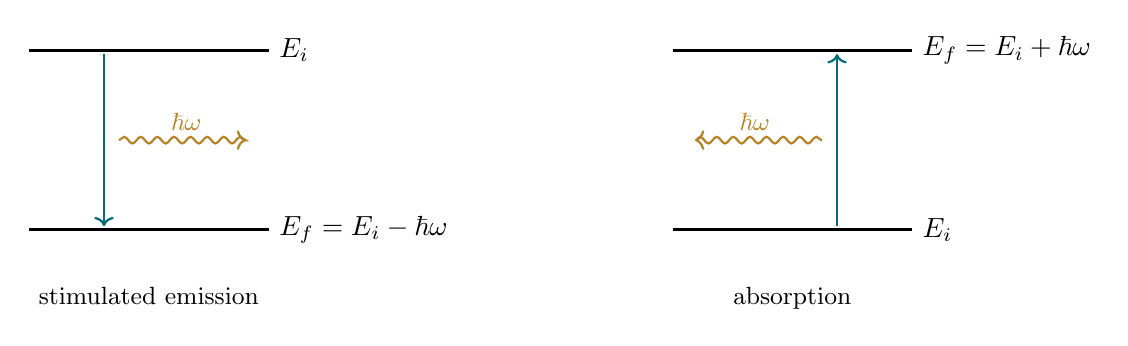
\begin{tikzpicture}[scale=0.95]
  % stimulated emission
  \draw[line width=1.1pt] (0,0.9) -- (3.2,0.9) node[right] {$E_i$};
  \draw[line width=1.1pt] (0,-1.5) -- (3.2,-1.5) node[right] {$E_f=E_i-\hbar\omega$};
  \draw[->,secondary,thick] (1.0,0.85) -- (1.0,-1.45);
  \draw[exframe,thick,decorate,decoration={snake,amplitude=1.2pt,segment length=6pt},->] (1.2,-0.3) -- (2.9,-0.3);
  \node[exframe,above] at (2.1,-0.3) {\small $\hbar\omega$};
  \node[below=6mm] at (1.6,-1.5) {\small stimulated emission};
  % absorption
  \draw[line width=1.1pt] (8.6,-1.5) -- (11.8,-1.5) node[right] {$E_i$};
  \draw[line width=1.1pt] (8.6,0.9) -- (11.8,0.9) node[right] {$E_f=E_i+\hbar\omega$};
  \draw[->,secondary,thick] (10.8,-1.45) -- (10.8,0.85);
  \draw[exframe,thick,decorate,decoration={snake,amplitude=1.2pt,segment length=6pt},<-] (8.9,-0.3) -- (10.6,-0.3);
  \node[exframe,above] at (9.7,-0.3) {\small $\hbar\omega$};
  \node[below=6mm] at (10.2,-1.5) {\small absorption};
\end{tikzpicture}
\end{center}

\textbf{*** Study Note (correction):} The notebook writes the prefactors of this section as $2\pi/\hbar^2$ and $4\pi/\hbar^2$ (probability) and $4\pi/\hbar$ (rates). For the sum of two terms each contribution has the same form as the single-term result: the probability of each term is $\frac4{\hbar^2}|\cdot|^2\sin^2(\cdot)/(\cdot)^2$ (which is exactly $\frac1{\hbar^2}|\cdot|^2\sin^2\alpha t/\alpha^2$), and the rate of each term is $2\pi/\hbar$, not $4\pi/\hbar$. Using $\lim_{t\to\infty}\sin^2(\Delta t/2)/\Delta^2=\frac{\pi t}2\delta(\Delta)$ gives $\frac4{\hbar^2}\cdot\frac\pi2=\frac{2\pi}{\hbar^2}$, which is the golden rule above.

For a continuum of final states the two processes give
\begin{align*}
W_{fi}^{\text{Emission}}&=\frac{2\pi}\hbar\,|\langle f|\hat v|i\rangle|^2\,\rho(E_i-\hbar\omega)\\
W_{fi}^{\text{Absorption}}&=\frac{2\pi}\hbar\,|\langle f|\hat v^\dagger|i\rangle|^2\,\rho(E_i+\hbar\omega)
\end{align*}
and for $\hat v=\hat v^\dagger$ their ratio is
\[
\frac{W_{fi}^{\text{Em}}}{W_{fi}^{\text{Ab}}}=\frac{\rho(E_i-\hbar\omega)}{\rho(E_i+\hbar\omega)}\qquad\text{(condition for balance)}
\]
\textbf{*** Study Note:} For $\hat v=\hat v^\dagger$ the matrix elements for emission and absorption are equal; the rates differ only because the density of final states is evaluated at different energies. This equality of the matrix elements is the quantum origin of $B_{ab}=B_{ba}$ in Section~\ref{td:sec:rad}.

\textbf{*** Common mistakes:} (a) writing $\delta(E_f-E_i-\hbar\omega)$ for emission (it is absorption; emission has $E_f=E_i-\hbar\omega$), (b) a factor of $2$ error when converting $\delta(\omega_{fi}-\omega)$ to $\delta(E)$ or $\delta(x/2)$ to $\delta(x)$, (c) forgetting that the rate needs the continuum $\rho(E_f)$ or a spread of frequencies.
%==============================================================================
\section{Adiabatic and Sudden Approximations: First-Order Treatment}
\label{td:sec:adsud}
%==============================================================================

\subsection{Slow and Fast Perturbations}
Take $\hat H=\hat H^0+\hat V(t)$, where $\hat V(t)$ is small in comparison with $\hat H^0$. The decisive question is the \textbf{rate of change} of $\hat V(t)$ compared with the natural time scale $1/\omega_{fi}$ of the system:

\begin{center}
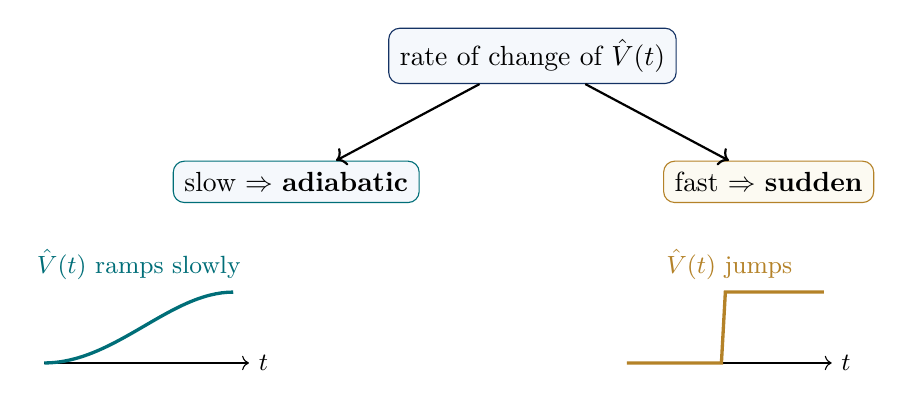
\begin{tikzpicture}[scale=1]
  \node[draw,rounded corners,fill=boxbg,draw=primary,inner sep=4pt] (a) at (0,0) {rate of change of $\hat V(t)$};
  \node[draw,rounded corners,fill=boxbg,draw=secondary,inner sep=4pt] (s) at (-3.0,-1.6) {slow $\Rightarrow$ \textbf{adiabatic}};
  \node[draw,rounded corners,fill=exbg,draw=exframe,inner sep=4pt] (f) at (3.0,-1.6) {fast $\Rightarrow$ \textbf{sudden}};
  \draw[->,thick] (a) -- (s); \draw[->,thick] (a) -- (f);
  % small sketches (added)
  \draw[->] (-6.2,-3.9) -- (-3.6,-3.9) node[right] {\small $t$};
  \draw[very thick,secondary] (-6.2,-3.9) .. controls (-5.3,-3.9) and (-4.6,-3.0) .. (-3.8,-3.0);
  \draw[->] (1.2,-3.9) -- (3.8,-3.9) node[right] {\small $t$};
  \draw[very thick,exframe] (1.2,-3.9) -- (2.4,-3.9) -- (2.45,-3.0) -- (3.7,-3.0);
  \node[secondary] at (-5.0,-2.65) {\small $\hat V(t)$ ramps slowly};
  \node[exframe] at (2.5,-2.65) {\small $\hat V(t)$ jumps};
\end{tikzpicture}
\end{center}
\textbf{*** Study Note (figure):} The tree is from the notebook; the two small sketches of $\hat V(t)$ were added to show what ``slow'' and ``fast'' mean.

Start from the first-order amplitude (initial state $|i\rangle$, final state $|f\rangle$, $t_0=0$):
\[
c_f^{(1)}(t)=-\frac i\hbar\int_0^tdt'\,\langle f|\hat V(t')|i\rangle\,e^{i\omega_{fi}t'}
\]
Use $e^{i\omega_{fi}t'}=\dfrac1{i\omega_{fi}}\dfrac\partial{\partial t'}e^{i\omega_{fi}t'}$ and integrate by parts:
\begin{align*}
c_f^{(1)}(t)&=-\frac i\hbar\cdot\frac1{i\omega_{fi}}\int_0^tdt'\,\langle f|\hat V(t')|i\rangle\,\frac\partial{\partial t'}e^{i\omega_{fi}t'}\\
&=-\frac1{\hbar\omega_{fi}}\Big\{\big[\langle f|\hat V(t')|i\rangle e^{i\omega_{fi}t'}\big]_0^t-\int_0^tdt'\,e^{i\omega_{fi}t'}\,\frac\partial{\partial t'}\langle f|\hat V(t')|i\rangle\Big\}
\end{align*}
With the boundary condition $\langle f|\hat V(t')|i\rangle=0$ at $t'=0$ and $t'=t$ (the perturbation is switched on and off smoothly), the boundary term vanishes:
\[
c_f^{(1)}(t)=\frac1{\hbar\omega_{fi}}\int_0^tdt'\,e^{i\omega_{fi}t'}\,\frac\partial{\partial t'}\langle f|\hat V(t')|i\rangle
\]
The amplitude is controlled by the \textit{time derivative} of the matrix element.

\subsection{Adiabatic Approximation}
For a slow process, $\dfrac\partial{\partial t}\langle f|\hat V(t)|i\rangle\to$ constant, which can be taken out of the integral:
\[
c_f^{(1)}(t)=\frac1{\hbar\omega_{fi}}\,\frac\partial{\partial t}\langle f|\hat V(t)|i\rangle\int_0^tdt'\,e^{i\omega_{fi}t'},\qquad
\Big|\int_0^tdt'\,e^{i\omega_{fi}t'}\Big|^2=\frac{\sin^2(\omega_{fi}t/2)}{(\omega_{fi}/2)^2}
\]
Then
\begin{align*}
P_{i\to f}(t)&=\frac1{\hbar^2\omega_{fi}^2}\Big|\frac\partial{\partial t}\langle f|\hat V(t)|i\rangle\Big|^2\,\frac{\sin^2(\omega_{fi}t/2)}{(\omega_{fi}/2)^2}\\
&=\frac4{\hbar^2\omega_{fi}^4}\Big|\frac\partial{\partial t}\langle f|\hat V(t)|i\rangle\Big|^2\sin^2\frac{\omega_{fi}t}2
\end{align*}
\begin{thm}{Adiabatic Approximation}
\[
P_{i\to f}^{\text{Adia}}=\frac4{\hbar^2\omega_{fi}^4}\Big|\frac\partial{\partial t}\langle f|\hat V(t)|i\rangle\Big|^2\sin^2\frac{\omega_{fi}t}2
\]
\end{thm}

\textbf{*** Intuition:} If the perturbation changes slowly compared with $1/\omega_{fi}$, the system has time to adjust and stays in the instantaneous eigenstate (the adiabatic theorem); the transition probability is small, of order $(\partial_tV/\hbar\omega_{fi}^2)^2$.

\textbf{*** Verification (dimensions):} $\partial_tV$ has units of energy per time and $\hbar\omega_{fi}^2$ has the same units, so the ratio $\partial_tV/\hbar\omega_{fi}^2$ is dimensionless and so is $P$.

\subsection{Sudden Approximation}
For a sudden (fast) change, $e^{i\omega_{fi}t'}\approx1$ during the change and cannot be pulled out as a slowly varying factor. Then the phase factor drops out of the modulus and
\[
P_{i\to f}=\frac1{\hbar^2\omega_{fi}^2}\,\big|e^{i\omega_{fi}t}\big|^2\Big|\int_0^tdt'\,\frac\partial{\partial t'}\langle f|\hat V(t')|i\rangle\Big|^2
\]
\begin{thm}{Sudden Approximation}
\[
P_{i\to f}=\frac1{\hbar^2\omega_{fi}^2}\Big|\int_0^tdt'\,\frac\partial{\partial t'}\langle f|\hat V(t')|i\rangle\Big|^2
\]
\end{thm}

\textbf{*** Study Note:} The integral of a derivative is the net \textit{change} $\Delta\langle f|\hat V|i\rangle$ of the matrix element across the rapid switching, so $P_{i\to f}\sim|\Delta\langle f|\hat V|i\rangle|^2/(\hbar\omega_{fi})^2$. The boundary term that was dropped above (it vanishes only for a smooth turn-on and turn-off) cannot be dropped for a genuine jump; keeping it only adds an oscillating factor of order unity, so the estimate stands as an order of magnitude. The complete, non-perturbative treatment of a sudden change is in Section~\ref{td:sec:sudden}.

\textbf{*** Exam Tip:} Compare the duration $T$ of the change with $1/\omega_{fi}$: $T\gg1/\omega_{fi}$ means adiabatic (no transitions, $P\propto(\partial_tV)^2$), $T\ll1/\omega_{fi}$ means sudden (the state is left unchanged and projected onto the new eigenstates).
%==============================================================================
\section{Emission and Absorption of Radiation}
\label{td:sec:rad}
%==============================================================================

\subsection{The Radiation Field and the Dipole Approximation}
Consider a plane electromagnetic wave
\[
\vec E(\vec r,t)=\vec E_0\exp\{i(\vec k\cdot\vec r-\omega t)\}
\]
with the wave vector $\vec k$ along $y$, the electric field along $z$ and the magnetic field along $x$.

\begin{center}
\begin{tikzpicture}[scale=1]
  \draw[->,gray] (0,0) -- (0,2.7) node[above] {$z$};
  \draw[->,gray] (0,0) -- (3.9,0) node[right] {$y$};
  \draw[->,gray] (0,0) -- (-1.7,-1.3) node[below left] {$x$};
  \draw[->,very thick,primary] (0,0) -- (0,2.1) node[right] {$\vec E$};
  \draw[->,very thick,exframe] (0,0) -- (-1.25,-0.95) node[above left] {$\vec B$};
  \draw[->,very thick,secondary] (0,0) -- (3.1,0);
  \node[secondary,above] at (1.9,0.0) {$\vec k$};
  \node[secondary,right] at (3.15,-0.4) {\small wave propagates};
\end{tikzpicture}
\end{center}

Two simplifications follow because the wavelength is much larger than the atom:
\begin{itemize}
    \item The \textbf{spatial variation} of $\vec E$ does not matter on the scale of the atom, so $\vec E$ is evaluated at the position of the atom (the \textbf{dipole approximation}).
    \item The \textbf{electric field} plays the crucial role here, not the magnetic field.
\end{itemize}
We take $\vec E=E_0\cos\omega t\,\hat e_3$, i.e.\ a wave polarized along $z$.

\textbf{*** Study Note:} The magnetic force on an electron is smaller than the electric force by a factor $v/c\sim\alpha$, and for optical wavelengths ($\gtrsim10^3$ atomic radii) $e^{i\vec k\cdot\vec r}\approx1$ across the atom. Corrections to the dipole approximation give magnetic dipole and electric quadrupole transitions, which are much weaker.

\subsection{Hamiltonian of the Atom in the Field}
For an atom with two levels $|\psi_a\rangle,|\psi_b\rangle$ ($E_b>E_a$, $\hbar\omega_0=E_b-E_a$) the time-dependent Hamiltonian is
\[
\hat H'(t)=-qE_0\,z\cos\omega t
\]
and its matrix elements are
\[
H'_{ba}=\langle\psi_b|\hat H'(t)|\psi_a\rangle=-qE_0\cos\omega t\,\langle\psi_b|z|\psi_a\rangle=-E_0\,p\cos\omega t
\]
where $p=q\langle\psi_b|z|\psi_a\rangle$ is the \textbf{dipole moment} (the dipole matrix element). The diagonal terms are zero.

\textbf{*** Complete Solution (why the diagonal terms vanish):} $\hat z$ is odd under parity and atomic stationary states have definite parity, so $|\psi_a|^2$ is even and $\langle\psi_a|z|\psi_a\rangle=\int z|\psi_a|^2d^3r=0$; the same holds for $b$.

\subsection{Absorption, Stimulated Emission and Spontaneous Emission}
Section~\ref{td:sec:two} gives, for the sinusoidal perturbation near resonance, with $V_{ba}=-E_0p$:
\[
P_{a\to b}(t)=\Big(\frac{|V_{ba}|}\hbar\Big)^2\frac{\sin^2\!\big[(\omega_0-\omega)\frac t2\big]}{(\omega_0-\omega)^2}
=\Big(\frac{pE_0}\hbar\Big)^2\frac{\sin^2\!\big[(\omega_0-\omega)\frac t2\big]}{(\omega_0-\omega)^2}
\]
\begin{itemize}
    \item \textbf{Absorption:} a photon is absorbed and the atom goes $a\to b$ with probability $P_{a\to b}$.
    \item \textbf{Stimulated emission:} an incident photon induces $b\to a$ and a second identical photon is emitted. By symmetry $P_{b\to a}$ has the same form (with $V_{ab}$).
    \item \textbf{Spontaneous emission:} the atom in $b$ drops to $a$ and emits a photon even with no field applied. It cannot come out of a classical-field calculation; it is obtained from Einstein's argument below.
\end{itemize}

\begin{center}
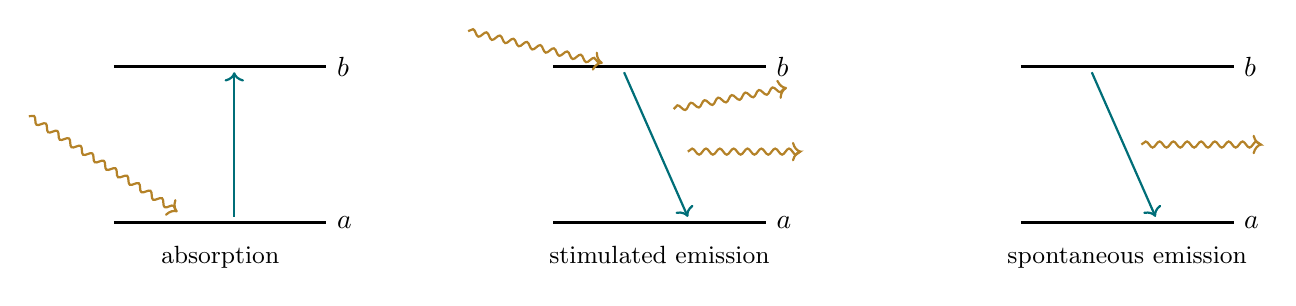
\begin{tikzpicture}[scale=0.9]
  \tikzset{wv/.style={exframe,thick,decorate,decoration={snake,amplitude=1.1pt,segment length=5pt}}}
  % absorption
  \draw[line width=1.1pt] (0,0) -- (3,0) node[right] {$a$};
  \draw[line width=1.1pt] (0,2.2) -- (3,2.2) node[right] {$b$};
  \draw[wv,->] (-1.2,1.5) -- (0.9,0.15);
  \draw[->,thick,secondary] (1.7,0.08) -- (1.7,2.12);
  \node[below,align=center] at (1.5,-0.2) {\small absorption};
  % stimulated emission
  \begin{scope}[xshift=6.2cm]
  \draw[line width=1.1pt] (0,0) -- (3,0) node[right] {$a$};
  \draw[line width=1.1pt] (0,2.2) -- (3,2.2) node[right] {$b$};
  \draw[wv,->] (-1.2,2.7) -- (0.7,2.25);
  \draw[->,thick,secondary] (1.0,2.12) -- (1.9,0.08);
  \draw[wv,->] (1.7,1.6) -- (3.3,1.9);
  \draw[wv,->] (1.9,1.0) -- (3.5,1.0);
  \node[below,align=center] at (1.5,-0.2) {\small stimulated emission};
  \end{scope}
  % spontaneous emission
  \begin{scope}[xshift=12.8cm]
  \draw[line width=1.1pt] (0,0) -- (3,0) node[right] {$a$};
  \draw[line width=1.1pt] (0,2.2) -- (3,2.2) node[right] {$b$};
  \draw[->,thick,secondary] (1.0,2.12) -- (1.9,0.08);
  \draw[wv,->] (1.7,1.1) -- (3.4,1.1);
  \node[below,align=center] at (1.5,-0.2) {\small spontaneous emission};
  \end{scope}
\end{tikzpicture}
\end{center}

\textbf{*** Study Note (factor 4):} The notebook first writes this probability with a prefactor $(2V_{ba}/\hbar)^2$ and a little later says ``forget 4''. The prefactor consistent with Section~\ref{td:sec:two} is $(V_{ba}/\hbar)^2=(pE_0/\hbar)^2$, and this is what is used below.

\subsection{Incoherent Perturbation: Broadband Radiation}
A thermal (incoherent) field contains many frequencies with random phases, so the transition probabilities for different frequencies add. The \textbf{energy density} of an electromagnetic wave is
\[
u=\frac{\epsilon_0E_0^2}2 \quad\Longrightarrow\quad E_0^2=\frac{2u}{\epsilon_0}
\]
With $V_{ab}=qE_0\langle\psi_a|z|\psi_b\rangle=E_0p$ the stimulated-emission probability is
\[
P_{b\to a}=\Big(\frac{pE_0}\hbar\Big)^2\frac{\sin^2[(\omega_0-\omega)\frac t2]}{(\omega_0-\omega)^2}
=\frac{2u}{\epsilon_0\hbar^2}\,|p|^2\,\frac{\sin^2[(\omega_0-\omega)\frac t2]}{(\omega_0-\omega)^2}
\]
Replace $u$ by $\rho(\omega)\,d\omega$, where $\rho(\omega)$ is the energy density per unit frequency, and integrate over all frequencies. The \textbf{total transition probability for stimulated emission} is
\[
P_{b\to a}=\frac2{\epsilon_0\hbar^2}\,|p|^2\int_0^\infty d\omega\,\rho(\omega)\,\frac{\sin^2[(\omega_0-\omega)\frac t2]}{(\omega_0-\omega)^2}
\simeq\frac2{\epsilon_0\hbar^2}\,|p|^2\,\rho(\omega_0)\int d\omega\,\frac{\sin^2[(\omega_0-\omega)\frac t2]}{(\omega_0-\omega)^2}
\]
because the integrand is sharply peaked at $\omega\approx\omega_0$ (so $\rho$ is evaluated at $\omega_0$ and the limits may be extended to $\pm\infty$). Substitute $x=(\omega_0-\omega)t/2$, $d\omega=-\tfrac2t\,dx$, $(\omega_0-\omega)^2=4x^2/t^2$:
\[
\int d\omega\,\frac{\sin^2[\ldots]}{(\omega_0-\omega)^2}=\frac t2\int_{-\infty}^{\infty}dx\,\frac{\sin^2x}{x^2}=\frac t2\,\pi
\]
Therefore
\[
P_{b\to a}=\frac{|p|^2}{\epsilon_0\hbar^2}\,\pi\,\rho(\omega_0)\,t
\]
and the transition rate is constant:
\begin{thm}{Transition Rate for Stimulated Emission (Polarized Wave)}
\[
R_{b\to a}=\frac{P_{b\to a}}t=\frac{\pi\,|\vec p\cdot\hat n|^2\,\rho(\omega_0)}{\epsilon_0\hbar^2}, \qquad \vec p=q\langle\psi_a|\vec r|\psi_b\rangle\ \ (\text{dipole matrix element})
\]
\end{thm}
Here the wave propagates along $z$ and its polarization $\hat n$ lies in the $xy$-plane, $\hat n=\cos\phi\,\hat e_1+\sin\phi\,\hat e_2$; the dipole matrix element has an arbitrary direction, $\vec p=p\sin\theta\,\hat e_2+p\cos\theta\,\hat e_3$, so that $\vec p\cdot\hat n=p\sin\theta\sin\phi$.

\begin{center}
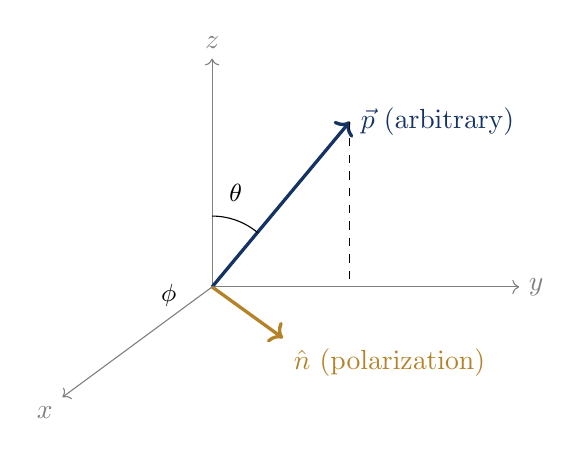
\begin{tikzpicture}[scale=1]
  \draw[->,gray] (0,0) -- (0,2.9) node[above] {$z$};
  \draw[->,gray] (0,0) -- (3.9,0) node[right] {$y$};
  \draw[->,gray] (0,0) -- (-1.9,-1.4) node[below left] {$x$};
  \draw[->,very thick,primary] (0,0) -- (1.75,2.1) node[right] {$\vec p$ (arbitrary)};
  \draw[dashed] (1.75,2.1) -- (1.75,0);
  \draw[->,very thick,exframe] (0,0) -- (0.9,-0.65) node[below right] {$\hat n$ (polarization)};
  \draw (0,0.9) arc (90:50:0.9); \node at (0.3,1.2) {\small $\theta$};
  \node at (-0.55,-0.1) {\small $\phi$};
\end{tikzpicture}
\end{center}

For an isotropic, unpolarized field average over directions:
\[
\big\langle|\vec p\cdot\hat n|^2\big\rangle=\frac1{4\pi}\iint|p|^2\sin^2\theta\sin^2\phi\,\sin\theta\,d\theta\,d\phi=\frac13|p|^2
\]
(the same for absorption). With this average:
\begin{thm}{Rate of Stimulated Emission (Isotropic Radiation)}
\[
R_{b\to a}=\frac{\pi\,|\vec p|^2\,\rho(\omega_0)}{3\,\epsilon_0\hbar^2}
\]
\end{thm}

\textbf{*** Complete Solution (the angular average):} $\int_0^\pi\sin^3\theta\,d\theta=\tfrac43$ and $\int_0^{2\pi}\sin^2\phi\,d\phi=\pi$, so $\frac1{4\pi}\cdot\frac43\cdot\pi=\frac13$ \checkmark. (The notebook writes $\vec p\cdot\hat n=p\sin\theta\cos\phi$ in one line and integrates $\sin^2\phi$; the average is $\tfrac13$ either way.)

\textbf{*** Verification:} The probability grows \textit{linearly} in $t$ here, unlike the $\sin^2$ oscillation for a single monochromatic wave. The linear growth (a rate) is exactly what the broad frequency distribution produces, as in the golden rule.

\textbf{*** Memory Rule:} Monochromatic: probability $\propto\sin^2(\cdot)/(\cdot)^2$ (oscillates); broadband: probability $\propto t$ (a constant rate).

\subsection{Spontaneous Emission: Einstein's \texorpdfstring{$A$}{A} and \texorpdfstring{$B$}{B} Coefficients}
Let $N_b$ atoms be in the upper state $|\psi_b\rangle$ and $N_a$ in the lower state $|\psi_a\rangle$. Define the coefficient $B_{ba}$ by the rate of stimulated emission per atom, $R_{b\to a}=B_{ba}\rho(\omega_0)$, and $B_{ab}$ by the absorption rate per atom, $B_{ab}\rho(\omega_0)$. From the rate above,
\[
B_{ba}=\frac{\pi}{3\epsilon_0\hbar^2}\,|\vec p|^2
\]
\begin{itemize}
    \item Number of atoms leaving the excited state by stimulated emission: $N_bB_{ba}\rho(\omega_0)$.
    \item Absorption: number of atoms joining the upper level $=N_aB_{ab}\rho(\omega_0)$.
    \item Let $A$ be the \textbf{spontaneous emission rate}: number of atoms leaving the upper level this way $=N_bA$.
\end{itemize}
So
\[
\frac{dN_b}{dt}=-N_bA-N_bB_{ba}\rho(\omega_0)+N_aB_{ab}\rho(\omega_0)
\]
At thermal equilibrium $dN_b/dt=0$:
\[
\rho(\omega_0)=\frac A{(N_a/N_b)B_{ab}-B_{ba}},\qquad
\frac{N_a}{N_b}=\frac{e^{-E_a/k_BT}}{e^{-E_b/k_BT}}=\exp\Big(\frac{\hbar\omega_0}{k_BT}\Big)
\]
\[
\rho(\omega_0)=\frac A{\exp\big(\frac{\hbar\omega_0}{k_BT}\big)B_{ab}-B_{ba}}
\]
This must agree with Planck's black-body law,
\[
\rho(\omega_0)=\frac{\hbar\omega_0^3}{\pi^2c^3}\;\frac1{\exp\big(\frac{\hbar\omega_0}{k_BT}\big)-1}
\]
Comparing the two (they must be equal at all temperatures):
\begin{thm}{Einstein Coefficients}
\[
B_{ab}=B_{ba},\qquad A=\frac{\hbar\omega_0^3}{\pi^2c^3}\,B_{ba}\ \ (\text{rate of spontaneous emission}),\qquad B_{ba}=\frac\pi{3\epsilon_0\hbar^2}|\vec p|^2
\]
\end{thm}
If only spontaneous emission acts (no absorption, no stimulated emission) then
\[
\frac{dN_b}{dt}=-N_bA\;\Longrightarrow\;N_b(t)=N_b(0)\,e^{-At},\qquad\boxed{\ \tau=\frac1A\ }\ \ \text{(lifetime of an excited state)}
\]
\textbf{*** Complete Solution (explicit $A$):}
\[
A=\frac{\hbar\omega_0^3}{\pi^2c^3}\cdot\frac{\pi|\vec p|^2}{3\epsilon_0\hbar^2}=\frac{\omega_0^3\,|\vec p|^2}{3\pi\epsilon_0\hbar c^3}
\]
\textbf{*** Verification (dimensions):} $[\omega_0^3|\vec p|^2]=\text{s}^{-3}\,\text{C}^2\text{m}^2$ and $[\epsilon_0\hbar c^3]=\dfrac{\text{C}^2}{\text{J m}}\cdot\text{J s}\cdot\dfrac{\text{m}^3}{\text{s}^3}=\text{C}^2\text{m}^2\text{s}^{-2}$, so $[A]=\text{s}^{-1}$ \checkmark.

\textbf{*** Verification (hydrogen $2p\to1s$):} here $\hbar\omega_0=\tfrac34\,(13.6\ \text{eV})$ and $|\vec p|^2=e^2\,|\langle1s|\vec r|2p\rangle|^2=e^2\,\dfrac{2^{15}}{3^{10}}\,a_0^2$. Inserting numbers in $A=\omega_0^3|\vec p|^2/(3\pi\epsilon_0\hbar c^3)$ gives $A\simeq6.3\times10^{8}\ \text{s}^{-1}$, i.e.\ $\tau=1/A\simeq1.6$ ns, the known lifetime of the hydrogen $2p$ state.

\textbf{*** Intuition:} A classical radiation field only gives absorption and stimulated emission. Equilibrium with black-body radiation (Planck's law) is impossible without a third process that occurs even in the absence of radiation, and that is spontaneous emission. Since $A\propto\omega_0^3|\vec p|^2$, high-frequency transitions with large dipole moments decay fastest.

\textbf{*** Exam Tip:} The route to remember: rate equation $\Rightarrow$ equilibrium $\Rightarrow$ Boltzmann ratio $e^{\hbar\omega_0/k_BT}$ $\Rightarrow$ compare with Planck $\Rightarrow$ $B_{ab}=B_{ba}$ and $A=\hbar\omega_0^3B/\pi^2c^3$.

\subsection{Selection Rules}
The excited-state lifetime depends on the dipole matrix element $\langle\psi_a|\vec r|\psi_b\rangle$. When is $\langle n'l'm'|\vec r|nlm\rangle\neq0$? (The notebook poses this as a question; the answer follows.) Use the commutation relations
\[
[\hat L_z,\hat x]=i\hbar\hat y,\qquad[\hat L_z,\hat y]=-i\hbar\hat x,\qquad[\hat L_z,\hat z]=0
\]
\paragraph{Selection rule for $m$.} For $\hat z$, $\langle n'l'm'|[\hat L_z,\hat z]|nlm\rangle=0$ gives $\hbar(m'-m)\langle n'l'm'|\hat z|nlm\rangle=0$. Hence
\begin{thm}{Selection Rule for $z$}
\[
\langle n'l'm'|\hat z|nlm\rangle\neq0\ \Longrightarrow\ m'=m
\]
\end{thm}
For $\hat x$ and $\hat y$:
\begin{align*}
\langle n'l'm'|[\hat L_z,\hat x]|nlm\rangle&=i\hbar\langle n'l'm'|\hat y|nlm\rangle\ \Longrightarrow\ (m'-m)\langle n'l'm'|\hat x|nlm\rangle=i\langle n'l'm'|\hat y|nlm\rangle \tag{A}\\
\langle n'l'm'|[\hat L_z,\hat y]|nlm\rangle&=-i\hbar\langle n'l'm'|\hat x|nlm\rangle\ \Longrightarrow\ (m'-m)\langle n'l'm'|\hat y|nlm\rangle=-i\langle n'l'm'|\hat x|nlm\rangle \tag{B}
\end{align*}
Multiply (A) by $(m'-m)$ and use (B):
\begin{align*}
(m'-m)^2\langle n'l'm'|\hat x|nlm\rangle&=i(m'-m)\langle n'l'm'|\hat y|nlm\rangle=\langle n'l'm'|\hat x|nlm\rangle\\
\Longrightarrow\ \big[(m'-m)^2-1\big]\langle n'l'm'|\hat x|nlm\rangle&=0
\end{align*}
The same holds for $\hat y$.
\begin{thm}{Selection Rule for $x$ and $y$}
\[
\langle n'l'm'|\hat x|nlm\rangle\neq0\ \text{(or }\hat y)\ \Longrightarrow\ m'-m=\pm1
\]
\end{thm}
\paragraph{Selection rule for $l$.} Use the identity
\[
\big[\hat L^2,[\hat L^2,\hat{\vec r}]\big]=2\hbar^2\big[\hat{\vec r}\hat L^2+\hat L^2\hat{\vec r}\big]
\]
and take its matrix element between $\langle n'l'm'|$ and $|nlm\rangle$. The left-hand side gives $\hbar^4[l'(l'+1)-l(l+1)]^2\langle\vec r\rangle$ and the right-hand side $2\hbar^4[l(l+1)+l'(l'+1)]\langle\vec r\rangle$, where $\langle\vec r\rangle=\langle n'l'm'|\hat{\vec r}|nlm\rangle$. Hence
\[
\Big\{2\big[l(l+1)+l'(l'+1)\big]-\big[l'(l'+1)-l(l+1)\big]^2\Big\}\langle n'l'm'|\hat{\vec r}|nlm\rangle=0
\]
The bracket factorizes:
\[
\big[(l'+l+1)^2-1\big]\big[(l'-l)^2-1\big]=0
\]
so a non-zero matrix element requires $l'=l=0$ or $l'-l=\pm1$.
\begin{thm}{Selection Rule for $l$ (Dipole Transitions)}
\[
\langle n'l'm'|\hat{\vec r}|nlm\rangle\neq0\ \Longrightarrow\ \Delta l=l'-l=\pm1\quad(\text{and }\Delta m=0,\pm1)
\]
\end{thm}

\textbf{*** Complete Solution (factorization):} Let $S=(l+l'+1)^2$ and $D=(l'-l)^2$. Then $2[l(l+1)+l'(l'+1)]=S+D-1$ and $[l'(l'+1)-l(l+1)]^2=SD$, so the bracket equals $S+D-1-SD=-(S-1)(D-1)$ \checkmark. The factor $S=1$ means $l+l'=0$, i.e.\ $l=l'=0$.

\textbf{*** Study Note (the case $l=l'=0$):} It is allowed by the factorization but excluded by parity: $\hat{\vec r}$ is odd and states of angular momentum $l$ have parity $(-1)^l$, so $\langle l'|\vec r|l\rangle\neq0$ needs $l+l'$ odd. Together with the commutator result this leaves only $\Delta l=\pm1$.

\textbf{*** Alternate method:} Parity alone shows that $\Delta l$ is odd; the double commutator identity (equivalently the Wigner--Eckart theorem for a vector operator) shows that it cannot exceed $1$ in magnitude.

\textbf{*** Exam Tip:} Electric dipole selection rules: $\Delta l=\pm1$, $\Delta m=0$ for light polarized along $z$ and $\Delta m=\pm1$ for $x,y$ (circular) polarization. Examples: $2p\to1s$ is allowed ($\Delta l=-1$), $2s\to1s$ and $3d\to1s$ are forbidden. A state with no allowed dipole decay is long-lived (\textbf{metastable}), since $A\propto|\vec p|^2=0$ at this order.

\textbf{*** Common mistakes:} (a) using $E_0^2=u/\epsilon_0$ instead of $2u/\epsilon_0$ (the $\frac12$ in $u=\epsilon_0E_0^2/2$), (b) forgetting the average factor $\frac13$ for isotropic radiation, (c) taking the stimulated emission rate for a monochromatic wave (oscillating) as a constant rate, (d) forgetting that $B_{ab}=B_{ba}$ for non-degenerate levels follows from equilibrium, not from an assumption.
%==============================================================================
\section{The Sudden Approximation: Overlap of Eigenstates}
\label{td:sec:sudden}
%==============================================================================

\subsection{Statement of the Approximation}
Now let the Hamiltonian change \textit{suddenly}, faster than any time scale of the system, so that the change need not be small. Let
\begin{align*}
\hat H^0|\phi_i\rangle&=\epsilon_i|\phi_i\rangle \qquad\text{(unperturbed, before the change)}\\
\hat H|\psi_n\rangle&=\tilde\epsilon_n|\psi_n\rangle \qquad\text{(perturbed, after the change)}
\end{align*}
Because the change is too fast for the state to respond, the system is still in $|\phi_i\rangle$ immediately afterwards. Expand it in the eigenstates of the new Hamiltonian:
\[
|\phi_i\rangle=\sum_nc_n|\psi_n\rangle,\qquad |\langle\psi_n|\phi_i\rangle|^2=|c_n|^2
\]
\begin{thm}{Sudden Approximation (Overlap Form)}
\[
P_{i\to n}=|\langle\psi_n|\phi_i\rangle|^2
\]
the probability of finding the system in the eigenstate $|\psi_n\rangle$ of the new Hamiltonian.
\end{thm}
For a weak sudden perturbation first-order perturbation theory gives the estimate
\[
P_{i\to f}\simeq\frac{|\langle\psi_f|\hat V'(t)|\psi_i\rangle|^2}{\hbar^2\omega_{fi}^2}
\]

\textbf{*** Study Note (correction):} The notebook writes the denominator as $\hbar^2\omega_{fi}$; the square on $\omega_{fi}$ is needed for $P$ to be dimensionless and agrees with Section~\ref{td:sec:adsud}.

\textbf{*** Verification:} If the change is a weak perturbation $\hat V$, the new eigenstate is $|\psi_f\rangle\simeq|\phi_f\rangle+\sum_{m\ne f}\frac{\langle\phi_m|\hat V|\phi_f\rangle}{\epsilon_f-\epsilon_m}|\phi_m\rangle$, so $\langle\psi_f|\phi_i\rangle\simeq\frac{\langle\phi_f|\hat V|\phi_i\rangle}{\epsilon_i-\epsilon_f}$ for $f\neq i$ and $P_{i\to f}=|\langle\phi_f|\hat V|\phi_i\rangle|^2/(\hbar\omega_{fi})^2$, in agreement.

\textbf{*** Intuition:} Sudden means ``the wavefunction has no time to move'': you freeze $|\phi_i\rangle$ and ask how much of it overlaps each new eigenstate. Adiabatic is the opposite limit: the state follows the changing eigenstate and $P\approx0$.

\subsection{Example: Beta Decay of Tritium}
\begin{prob}{Example: Tritium to Helium, $^{3}_{1}\text{H}\to{}^{3}_{2}\text{He}$}
Tritium $^3_1$H is hydrogen-like. Before the decay the electron is in the hydrogen ground state:
\[
\hat H^0=\frac{\hat p^2}{2m}-\frac{e^2}r,\qquad \phi_{1s}(\vec r)=\sqrt{\frac1{\pi a_0^3}}\,\exp\Big(-\frac r{a_0}\Big)
\]
The nucleus decays by beta decay,
\[
{}^3_1\text{H}\;\xrightarrow{\ \text{decay}\ }\;{}^3_2\text{He}+e^-+\bar\nu_e\qquad(\bar\nu_e:\ \text{antineutrino})
\]
The emitted electron leaves so fast that the nuclear charge changes suddenly from $Z=1$ to $Z=2$. For the one remaining electron in the helium ion,
\[
\hat H=\frac{\hat p^2}{2m}-\frac{2e^2}r,\qquad \psi_{1s}=\sqrt{\frac8{\pi a_0^3}}\,\exp\Big(-\frac{2r}{a_0}\Big)
\]
The probability to be in the ground state of the new ion is
\[
P=|\langle\psi_{1s}|\phi_{1s}\rangle|^2
\]
\end{prob}
\begin{prob}{Example: Tritium to Helium (completed)}
\textbf{*** Complete Solution:} Both functions are spherically symmetric, so
\begin{align*}
\langle\psi_{1s}|\phi_{1s}\rangle&=4\pi\int_0^\infty r^2dr\,\sqrt{\frac8{\pi a_0^3}}\sqrt{\frac1{\pi a_0^3}}\,e^{-3r/a_0}
=\frac{4\sqrt8}{a_0^3}\int_0^\infty r^2e^{-3r/a_0}dr\\
&=\frac{4\sqrt8}{a_0^3}\cdot\frac{2a_0^3}{27}=\frac{8\sqrt8}{27}=\frac{16\sqrt2}{27}\simeq0.838
\end{align*}
using $\int_0^\infty r^2e^{-\kappa r}dr=2/\kappa^3$ with $\kappa=3/a_0$. Hence
\[
\boxed{P=\Big(\frac{16\sqrt2}{27}\Big)^2=\frac{512}{729}\simeq0.70}
\]
The remaining $217/729\simeq0.30$ goes into excited bound states and the continuum (ionization).

\textbf{*** Verification:} Both states are normalized: $\frac4{a_0^3}\int r^2e^{-2r/a_0}dr=\frac4{a_0^3}\cdot\frac{a_0^3}4=1$ and $\frac{32}{a_0^3}\int r^2e^{-4r/a_0}dr=\frac{32}{a_0^3}\cdot\frac{a_0^3}{32}=1$ \checkmark. For $1s$ orbitals of charges $Z_1\to Z_2$ the same steps give $\langle\psi|\phi\rangle=8(Z_1Z_2)^{3/2}/(Z_1+Z_2)^3$, which is $1$ for $Z_1=Z_2$ (no change) and $8\cdot2^{3/2}/27$ for $1\to2$ \checkmark.
\end{prob}

\begin{center}
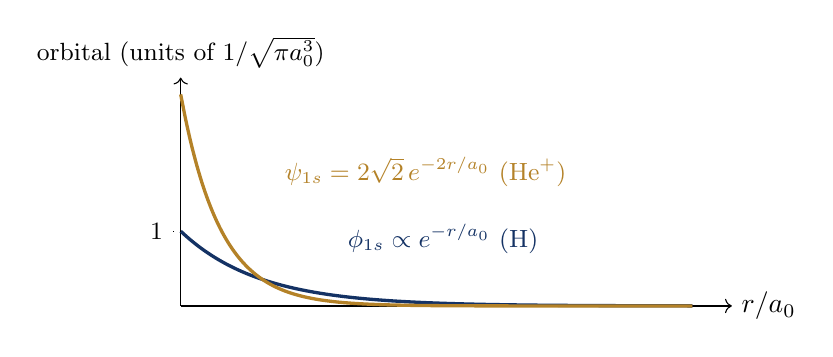
\begin{tikzpicture}[scale=1]
  \draw[->] (0,0) -- (7.0,0) node[right] {$r/a_0$};
  \draw[->] (0,0) -- (0,2.9) node[above] {\small orbital (units of $1/\sqrt{\pi a_0^3}$)};
  \draw[very thick,primary,domain=0:6.5,samples=100,smooth] plot (\x*1.0,{0.95*exp(-\x)});
  \draw[very thick,exframe,domain=0:6.5,samples=100,smooth] plot (\x*1.0,{0.95*2.8284*exp(-2*\x)});
  \node[primary,right] at (2.0,0.85) {\small $\phi_{1s}\propto e^{-r/a_0}$ (H)};
  \node[exframe,right] at (1.2,1.7) {\small $\psi_{1s}=2\sqrt2\,e^{-2r/a_0}$ (He$^+$)};
  \draw[dotted] (0,0.95) -- (-0.1,0.95) node[left] {\small $1$};
\end{tikzpicture}
\end{center}
\textbf{*** Study Note (figure):} The He$^+$ orbital is more compact (the nucleus now pulls twice as hard), so the old and new orbitals overlap only partly; this overlap, squared, is the probability $512/729$.

\textbf{*** Exam Tip:} Sudden approximation recipe: (i) write the initial eigenstate of the old Hamiltonian, (ii) write the eigenstates of the new Hamiltonian, (iii) the probability of landing in $|\psi_n\rangle$ is $|\langle\psi_n|\phi_i\rangle|^2$. Check that $\sum_n P_n=1$ (completeness) if asked for the total.
%==============================================================================
\section{Time Translation and Conservation of Energy}
%==============================================================================

\subsection{The Time-Translation Operator}
The Hamiltonian generates translations in time. For an infinitesimal step $\delta t$,
\[
\hat U_T(\delta t)=\Big(\mathbb 1-\frac i\hbar\hat H\,\delta t\Big)
\]
Starting a short step $\epsilon$ from two different times $t_1$ and $t_2$:
\begin{align*}
|\psi(t_1+\epsilon)\rangle&=\Big(\mathbb 1-\frac{i\epsilon}{\hbar}\hat H(t_1)\Big)|\psi_0\rangle\\
|\psi(t_2+\epsilon)\rangle&=\Big(\mathbb 1-\frac{i\epsilon}{\hbar}\hat H(t_2)\Big)|\psi_0\rangle
\end{align*}
If $\hat H$ has no explicit time dependence, $\hat H(t_1)=\hat H(t_2)$ and the same operator evolves the state no matter when the step starts: the physics is invariant under \textbf{time translation}.

\textbf{*** Study Note:} Here $|\psi_0\rangle$ stands for the state at the start of each short interval. The infinitesimal form is just the Schr\"odinger equation, $|\psi(t+\delta t)\rangle=|\psi(t)\rangle+\delta t\,\partial_t|\psi\rangle=\big(\mathbb 1-\frac i\hbar\hat H\delta t\big)|\psi(t)\rangle$, and repeating it gives $e^{-i\hat Ht/\hbar}$.

\subsection{Conservation of Energy}
The expectation value of an observable $\hat\Omega$ (with no explicit time dependence) obeys
\[
i\hbar\,\frac d{dt}\langle\hat\Omega\rangle=\big\langle[\hat\Omega,\hat H]\big\rangle
\]
Choose $\hat\Omega=\hat H$. Since $[\hat H,\hat H]=0$,
\begin{thm}{Conservation of Energy}
\[
i\hbar\,\frac d{dt}\langle\hat H\rangle=0\quad\Longrightarrow\quad\text{energy is conserved}
\]
\end{thm}

\textbf{*** Complete Solution (the commutator rule):} With $i\hbar|\dot\psi\rangle=\hat H|\psi\rangle$ and $-i\hbar\langle\dot\psi|=\langle\psi|\hat H$,
\[
\frac d{dt}\langle\psi|\hat\Omega|\psi\rangle=\langle\dot\psi|\hat\Omega|\psi\rangle+\langle\psi|\hat\Omega|\dot\psi\rangle=\frac i\hbar\langle\hat H\hat\Omega-\hat\Omega\hat H\rangle=-\frac i\hbar\langle[\hat\Omega,\hat H]\rangle
\]
which is $i\hbar\,\frac d{dt}\langle\hat\Omega\rangle=\langle[\hat\Omega,\hat H]\rangle$ \checkmark.

\textbf{*** Study Note (link to the rest of the chapter):} Time-translation invariance ($\hat H$ time-independent) is equivalent to conservation of energy. A time-dependent perturbation breaks the invariance: in general $\frac d{dt}\langle\hat H\rangle=\big\langle\frac{\partial\hat H}{\partial t}\big\rangle\neq0$, and the atom exchanges energy with the driving field. For a harmonic perturbation the exchanged amount is exactly $\hbar\omega$, which is the content of the $\delta(E_f-E_i\mp\hbar\omega)$ in Fermi's golden rule; for a constant perturbation ($\omega=0$) the same rule gives $E_f=E_i$.

\textbf{*** Memory Rule:} Time-independent $\hat H\Rightarrow$ energy conserved; periodic perturbation of frequency $\omega\Rightarrow$ energy changes only in quanta $\hbar\omega$.

\end{document}
